%\documentclass[a4paper, oneside, openany]{book}
\documentclass[a4paper]{article}

%**************************************************************
% Importazione package
%************************************************************** 

% modifica i margini
%\usepackage[top=3.1cm, bottom=3.1cm, left=2.2cm, right=2.2cm]{geometry}

% specifica con quale codifica bisogna leggere i file
\usepackage[utf8]{inputenc}

% per scrivere in italiano e in inglese;
% l'ultima lingua (l'italiano) risulta predefinita
\usepackage[english, italian]{babel}

% imposta lo stile italiano per i paragrafi
\usepackage{parskip}

% numera anche i paragrafi
\setcounter{secnumdepth}{4}

% elenca anche i paragrafi nell'indice
\setcounter{tocdepth}{4}

% permetti di definire dei colori
\usepackage[usenames,dvipsnames]{color}

% permette l'inserimento di url e di altri tipi di collegamento
\usepackage[colorlinks=true]{hyperref}

\hypersetup{
    colorlinks=true, % false: boxed links; true: colored links
    citecolor=black,
    filecolor=black,
    linkcolor=black, % color of internal links
    urlcolor=Maroon  % color of external links
}

% permette al comando \url{...} di andare a capo a metà di un link
\usepackage{breakurl}

% immagini
\usepackage{graphicx}

% permette di riferirsi all'ultima pagina con \pageref{LastPage}
\usepackage{lastpage}

% tabelle su più pagine
\usepackage{longtable}

% tabelle con il campo X per riempire lo spazio rimanente sulla riga
\usepackage{tabularx}

% personalizza l'intestazione e piè di pagina
\usepackage{fancyhdr}

% permette di inserire caratteri speciali
\usepackage{textcomp}

\fancypagestyle{plain}{
	% cancella tutti i campi di intestazione e piè di pagina
	\fancyhf{}

	\lhead{\GroupName{} \texttwelveudash \ProjectName{}}
	\chead{}
	\rhead{\slshape \leftmark}

	\lfoot{\DocTitle \\ v\DocVersion}
	\rfoot{\thepage\ di \pageref{LastPage}}

	% Visualizza una linea orizzontale in cima e in fondo alla pagina
	\renewcommand{\headrulewidth}{0.3pt}
	\renewcommand{\footrulewidth}{0.3pt}
}
\pagestyle{plain}

% Per inserire del codice sorgente formattato
\usepackage{listings}

\lstset{
  extendedchars=true,          % lets you use non-ASCII characters
  inputencoding=utf8,   % converte i caratteri utf8 in latin1, richiede \usepackage{listingsutf8} anzichè listings
  basicstyle=\ttfamily,        % the size of the fonts that are used for the code
  breakatwhitespace=false,     % sets if automatic breaks should only happen at whitespace
  breaklines=true,             % sets automatic line breaking
  captionpos=t,                % sets the caption-position to top
  commentstyle=\color{mygreen},   % comment style
  frame=none,               % adds a frame around the code
  keepspaces=true,            % keeps spaces in text, useful for keeping indentation of code (possibly needs columns=flexible)
  keywordstyle=\bfseries,     % keyword style
  numbers=none,               % where to put the line-numbers; possible values are (none, left, right)
  numbersep=5pt,              % how far the line-numbers are from the code
  numberstyle=\color{mygray}, % the style that is used for the line-numbers
  rulecolor=\color{black},    % if not set, the frame-color may be changed on line-breaks within not-black text (e.g. comments (green here))
  showspaces=false,           % show spaces everywhere adding particular underscores; it overrides 'showstringspaces'
  showstringspaces=false,     % underline spaces within strings only
  showtabs=false,             % show tabs within strings adding particular underscores
  stepnumber=5,               % the step between two line-numbers. If it's 1, each line will be numbered
  stringstyle=\color{red},    % string literal style
  tabsize=4,                  % sets default tabsize
  firstnumber=1      % visualizza i numeri dalla prima linea
}

% Permetti di utilizzare il grassetto per i caratteri Typewriter (per es. il font di \code{...} e \file{...})
\usepackage[T1]{fontenc}
\usepackage{lmodern}
%%%%%%%%%%%%%%
%  COSTANTI  %
%%%%%%%%%%%%%%

% In questa prima parte vanno definite le 'costanti' utilizzate da due o più documenti.

\newcommand{\GroupName}{\emph{SteakHolders}}
\newcommand{\ProjectName}{\emph{MaaP}}

\newcommand{\Proponente}{CoffeeStrap}
\newcommand{\Committente}{Prof. Tullio Vardanega}

% TODO I seguenti 4 sono deprecati, sono da togliere.
% Usare i 4 definiti sopra, con la maiuscola all'inizio!
\newcommand{\groupName}{\GroupName{}- FIXME: DEPRECATO}
\newcommand{\projectName}{\ProjectName{}- FIXME: DEPRECATO}
\newcommand{\proponente}{\Proponente{}- FIXME: DEPRECATO}
\newcommand{\committente}{\Committente{}- FIXME: DEPRECATO}

% La versione dei documenti deve essere definita qui in global, perchè serve anche agli altri documenti
\newcommand{\VersioneG}{??.??.??}
\newcommand{\VersionePQ}{??.??.??}
\newcommand{\VersioneNP}{1.1.5}
\newcommand{\VersioneAR}{1.1.1}

% Quando serve riferirsi a ``Nome del Documento + ultima versione x.y.z'' usiamo queste costanti:
\newcommand{\Glossario}{\emph{Glossario v\VersioneG{}}}
\newcommand{\PianoDiQualifica}{\emph{Piano di Qualifica v\VersionePQ{}}}
\newcommand{\NormeDiProgetto}{\emph{Norme di Progetto v\VersioneNP}}

\newcommand{\ScopoDelProdotto}{
	Lo scopo del progetto è la realizzazione di un \glossario{framework} per generare interfacce web di amministrazione dei dati di \glossario{business} basato su \glossario{stack} \glossario{Node.js} e \glossario{MondoDB}. L'obbiettivo è quello di semplificare il processo di implementazione di tali interfacce che lo sviluppatore, appoggiandosi alla produttività del framework MaaP, potrà generare in maniera semplice e veloce ottenendo quindi un considerevole risparmio di tempo e di sforzo. Il fruitore finale delle pagine generate sarà infine l'esperto di business che potrà visualizzare, gestire e modificare le varie entità e dati residenti in \glossario{MongoDB}.
	Il prodotto atteso si chiama \glossario{MaaP} ossia \emph{MongoDB as an admin Platform}.
}

%%%%%%%%%%%%%%
%  FUNZIONI  %
%%%%%%%%%%%%%%

% In questa seconda parte vanno definite le 'funzioni' utilizzate da due o più documenti.

% Serve a dare la giusta formattazione alle parole presenti nel glossario
% il nome del comando \glossary è già usato da LaTeX
\newcommand{\glossario}[1]{\mbox{#1\ped{\ped{G}}}}

% Serve a dare la giusta formattazione al codice inline
\newcommand{\code}[1]{\texttt{#1}}

% Serve a dare la giusta formattazione a tutte le path presenti nei documenti
\newcommand{\file}[1]{\texttt{#1}}

% Permette di andare a capo all'interno di una cella in una tabella
\newcommand{\multiLineCell}[2][c]{\begin{tabular}[#1]{@{}l@{}}#2\end{tabular}}

% Genera automaticamente la pagina di copertina
\newcommand{\makeFrontPage}{
  \begin{titlepage}
  \begin{center}

  \begin{center}
  
\includegraphics[width=10cm]{../../modello/steakman.png}
  \end{center}
  
  \vspace{33pt}

  \begin{Huge}
  \textbf{\DocTitle{}}
  \end{Huge}
  
  \textbf{\emph{Gruppo} \GroupName{} \, \texttwelveudash \, \emph{Progetto} \ProjectName{}}
  
  \vspace{11pt}

  \bgroup
  \def\arraystretch{2}
  \begin{tabular}{ r|l }
    \multicolumn{2}{c}{\textbf{Informazioni sul documento}} \\
    \hline
    \textbf{Versione} & \DocVersion{} \\
    \textbf{Redazione} & \multiLineCell[t]{\DocRedazione{}} \\
    \textbf{Verifica} & \multiLineCell[t]{\DocVerifica{}} \\
    \textbf{Approvazione} & \multiLineCell[t]{\DocApprovazione{}} \\
    \textbf{Uso} & \DocUso{} \\
    \textbf{Distribuzione} & \multiLineCell[t]{\DocDistribuzione{}} \\
  \end{tabular}
  \egroup

  \vspace{22pt}

  \textbf{Descrizione} \\
  \DocDescription{}

  \end{center}
  \end{titlepage}
}

%%%%%%%%%%%%%%
%  COSTANTI  %
%%%%%%%%%%%%%%

% In questa prima parte vanno definite le 'costanti' utilizzate soltanto da questo documento.
% Devono iniziare con una lettera maiuscola per distinguersi dalle funzioni.

\newcommand{\DocTitle}{Norme di Progetto}
\newcommand{\DocVersion}{\VersioneNP{}}
\newcommand{\DocRedazione}{
	Federico Poli \\
	Luca De Franceschi \\
	Giacomo Fornari \\
	Nicolò Tresoldi
}
\newcommand{\DocVerifica}{Serena Girardi}
\newcommand{\DocApprovazione}{Nicolò Tresoldi}
\newcommand{\DocUso}{Interno}
\newcommand{\DocDistribuzione}{
	\Committente{} \\
	Gruppo \GroupName{}
}

% La descrizione del documento
\newcommand{\DocDescription}{
 Questo documento descrive le regole, gli strumenti e le procedure adottate dal gruppo \GroupName{} per la realizzazione del progetto \ProjectName{}.
}

%%%%%%%%%%%%%%
%  FUNZIONI  %
%%%%%%%%%%%%%%

% In questa seconda parte vanno definite le 'funzioni' utilizzate soltanto da questo documento.

\DeclareUnicodeCharacter{00A0}{ }

\begin{document}

\makeFrontPage

\section*{Registro delle modifiche}

\small{
\begin{tabularx}{\textwidth}{|c|c|l|X|}
 \hline \textbf{Versione} & \textbf{Data} & \textbf{Persone coinvolte} & \textbf{Descrizione} \\

 % IN ORDINE DALLA MODIFICA PIÙ RECENTE ALLA PIÙ VECCHIA
 % TODO Compilarlo in modo verosimile riferendosi alle date del Piano di Progetto
 
 \hline 1.1.5 & 2013-12-05 & Nome Cognome &
 Stesura dello scheletro iniziale e del capitolo ``Introduzione''.\\

 \hline 1.1.4 & 2013-12-06 & Nome Cognome &
 ...\\

 \hline 1.1.3 & 2013-12-08 & Nome Cognome &
 ...\\

 \hline 1.1.2 & 2013-12-09 & Nome Cognome &
 ...\\

 \hline 1.1.1 & 2013-12-10 & Nome Cognome &
 ...\\

 \hline
\end{tabularx}
}


\clearpage

\tableofcontents
%\listoftables % non ci sono tabelle
%\listoffigures % non ci sono figure

\clearpage
\section{Introduzione}

\subsection{Scopo del documento}

Questo documento ha come obiettivo quello di definire le regole, gli strumenti e le procedure che tutti i membri del team dovranno adottare per l'intero svolgimento del progetto. Tutti i componenti del gruppo sono obbligati a visionare tale documento e ad applicare quanto scritto al fine di mantenere omogeneità e coesione in ogni aspetto del progetto.

Qualora vengano apportate modifiche o aggiunte al presente documento sarà necessario informare tempestivamente ogni membro del gruppo.

\subsection{Ambiguità}

Al fine di evitare ogni ambiguità relativa al linguaggio impiegato nei documenti viene fornito il \Glossario{}, contenente la definizione dei termini marcati con una G pedice.


\section{Tecnologie utilizzate}


L'architettura è stata progettata utilizzando diverse tecnologie, alcune delle quali espressamente richieste nel capitolato d'appalto. Vengono di seguito elencate e descritte le principali tecnologie impiegate e le motivazioni del loro utilizzo.

\begin{itemize}
	\item \textbf{Node.js}: piattaforma per il \glossario{back-end};
	\item \textbf{Express.js}: framework per la realizzazione dell’applicazione web in \glossario{Node.js};
	\item \textbf{MongoDB}: database di tipo \glossario{NoSQL} per la parte di recupero e salvataggio dei dati;
	\item \textbf{Mongoose}: libreria per interfacciarsi con il driver di \textbf{MongoDB};
	\item \textbf{Angular.js}: framework \glossario{JavaScript} la realizzazione del \glossario{front-end}.
\end{itemize}

\subsection{Node.js}
\textbf{Node.js} è una \glossario{piattaforma} software costruita sul motore JavaScript di Chrome che permette di realizzare facilmente applicazioni di rete scalabili e veloci. \textbf{Node.js} utilizza \textbf{JavaScript} come linguaggio di programmazione, e grazie al suo modello event-driver con chiamate di I/O non bloccanti risulta essere leggero e efficiente.

I principali vantaggi dell'utilizzo di \glossario{Node.js} sono:
\begin{itemize}
	\item \textbf{Approccio asincrono}: \glossario{Node.js} permette di accedere alle risorse del sistema operativo in modalità event-driven e non sfruttando il classico modello basato su processi o thread concorrenti utilizzato dai classici web server. Ciò garantisce una maggiore efficienza in termini di prestazioni, poiché durante le attese il runtime può gestire qualcos’altro in maniera asincrona.
	\item \textbf{Architettura modulare}: Lavorando con \glossario{Node.js} è molto facile organizzare il lavoro in librerie, importare i moduli e combinarli fra loro. Questo è reso molto comodo attraverso il \emph{node package manager} (\textbf{npm}) attraverso il quale lo sviluppatore può contribuire e accedere ai \glossario{package} messi a disposizione dalla community.
\end{itemize}

\subsection{Express.js}
\textbf{Express.js} è un \glossario{framework} minimale per creare applicazioni web con \glossario{Node.js}. Richiede moduli Node di terze parti per applicazioni che prevedono l’interazione con le basi di dati. \\
È stato utilizzato il \glossario{framework} Express.js per supportare lo sviluppo dell'application server grazie alle utili e robuste features da esso offerte, le quali sono pensate per non oscurare le funzionalità fornite da \glossario{Node.js} aprendo così le porte all'utilizzo di moduli per \glossario{Node.js} atti a supportare specifiche funzionalità.

\subsection{MongoDB}
\textbf{MongoDB} è un database \glossario{NoSQL} \glossario{open source} scalabile e altamente performante di tipo document-oriented, in cui i dati sono archiviati sotto forma di documenti in stile \glossario{JSON} con schemi dinamici, secondo una struttura semplice e potente.

I principali vantaggi derivati dal suo utilizzo sono:
\begin{itemize}
	\item \textbf{Alte performance}: non ci sono \emph{join} che possono rallentare le operazioni di lettura o scrittura. L’indicizzazione include gli indici di chiave anche sui documenti innestati e sugli array, permettendo una rapida interrogazione al database;
	\item \textbf{Affidabilità}: alto meccanismo di replicazione su server;
	\item \textbf{Schemaless}: non esiste nessuno \glossario{schema}, è più flessibile e può essere facilmente trasposto in un modello ad oggetti;
	\item Permette di definire query complesse utilizzando un linguaggio che non è \glossario{SQL};
	\item Permette di processare parallelamente i dati (\glossario{Map-Reduce});
	\item Tipi di dato più flessibili.
\end{itemize}

\subsection{Mongoose}
\textbf{Mongoose} è una libreria per interfacciarsi a \glossario{MongoDB} che permette di definire degli schemi per modellare i dati del database, imponendo una certa struttura per la creazione di nuovi \glossario{Document}. Inoltre fornisce molti strumenti utili per la validazione dei dati, per la definizione di query e per il cast dei tipi predefiniti.

Per interfacciare l'application server con \glossario{MongoDB} sono disponibili diversi progetti \glossario{open source}. Per questo progetto è stato scelto di utilizzare \glossario{Mongoose.js}, attualmente il più diffuso.
\section{Descrizione architettura}
% Nell'indice proposto da Tullio c'è:
% a. Metodo e formalismo di specifica
% b. Presentazione dell'architettura generale del sistema e identificazione dei componenti architetturali di alto livello

\subsection{Metodo e formalismo di specifica}

Le scelte progettuali per lo sviluppo di \ProjectName{} sono state fortemente influenzate dallo stack tecnologico utilizzato.

In primo luogo il progetto è basato su Node.js ed è scritto quindi in JavaScript: un linguaggio che è (tra le altre caratteristiche) orientato agli oggetti (\glossario{OOP}), ma che lascia grande libertà al programmatore nella scelta della tecnica da utilizzare per l'implementazione di pattern come l'\glossario{incapsulamento} e l'\glossario{ereditarietà}. Al contrario di altri linguaggi (C++, Java) non c'è un costrutto esplicito con il quale il programmatore può definire classi. 

Progettare il sistema con un'architettura ad oggetti classica non permette di rappresentare in modo immediato la gestione dinamica dei tipi e le caratteristiche tipiche degli stili di programmazione funzionali. In certi casi è stato necessario introdurre interfacce ``fittizie'', che non verranno codificate. Dato che questo introduce numerosi schematismi che appesantiscono i diagrammi e che non sono richiesti dal linguaggio di programmazione, si è cercato di limitarli soltanto ai casi in cui sono particolarmente utili.

Il nostro approccio alla progettazione è stato contemporaneamente top-down e bottom-up. Da un lato siamo partiti suddividendo il sistema in front-end e back-end, definendo l'interfaccia di comunicazione, scegliendo di seguire in ciascuno l'organizzazione suggeritaci dai framework (Express e AngularJS). Dall'altro lato siamo partiti dal basso, componendo e cercando di riutilizzare il più possibile le librerie già esistenti. Per far questo abbiamo prima cercato e confrontato con attenzione la struttura e le scelte sia di progetti open-source che di progetti proposti come best-practise.

L'approccio top-down è stato schematizzato nei diagrammi di deployment e dei package. Per la costruzione dei diagrammi delle classi, invece, questo approccio si è rivelato essere molto poco produttivo e rigoroso. I diagrammi delle classi proposti sono quindi \emph{uno dei possibili diagrammi} che descrivono l'applicazione, qualsiasi gerarchia o relazione complicata tra le classi verrebbe tradotta pressapoco nello stesso codice.

Per descrivere il sistema si è rivelato molto più comodo utilizzare i diagrammi di sequenza e di attività in un approccio bottom-up, descrivendo l'interazione tra i singoli oggetti senza preoccuparci della loro classificazione. In questo modo siamo anche riusciti a descrivere alcuni dei meccanismi tipici dell'applicazione, in particolar modo l'ordine in cui agiscono i \glossario{middleware} di Express. Riteniamo che saranno molto utili per la progettazione di dettaglio e per la codifica.

I diagrammi di deployment, dei \glossario{package}, delle classi, di sequenza e di attività presentati di seguito utilizzano la specifica \glossario{UML} 2.0.

\subsection{Architettura generale}

L'architettura del progetto si suddivide innanzitutto in una componente Client, costituita dal browser degli utenti che interagiranno con il \glossario{front-end} dell'applicazione, e in un web server, su cui verrà posto il \glossario{back-end}. Il server che ospita i database (la cui configurazione non è compito del progetto) non è necessario che risieda sullo stesso nodo su cui è posto il \glossario{back-end}.

\begin{figure}[H]
\centering
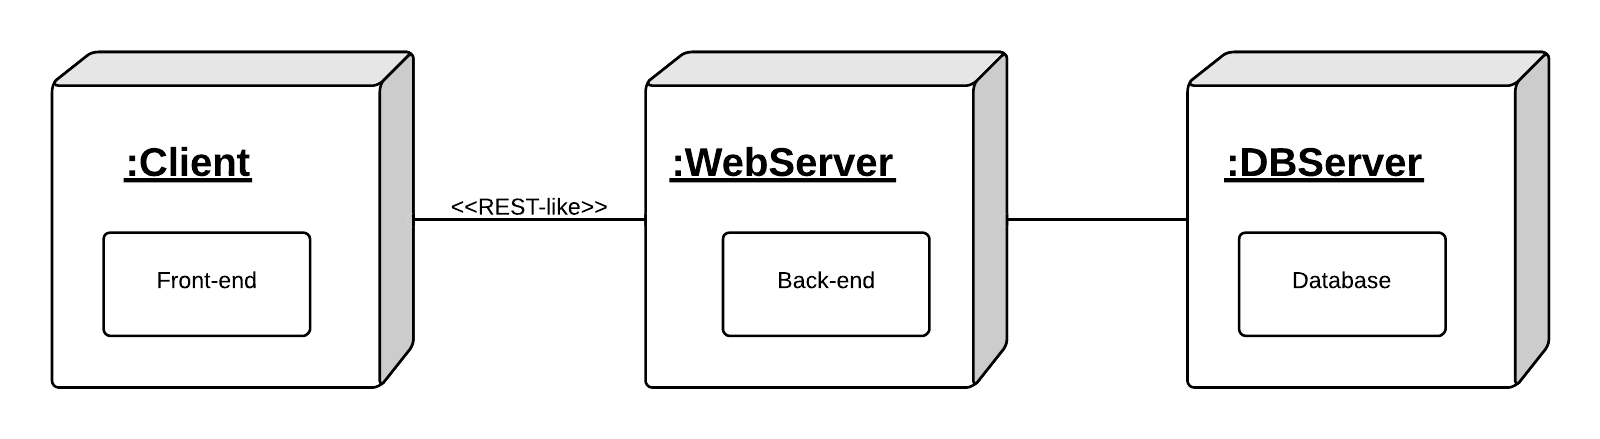
\includegraphics[width=\textwidth]{uml/diagramma-deployment.png}
\caption{Diagramma di deployment}
\end{figure}

\subsection{Interfaccia REST-like}
Per l'interfaccia della componente Back-end di \ProjectName{} si è scelto di utilizzare uno stile \glossario{REST-like}, ovvero basato sullo stile \glossario{REST} ma modificato per permettere l'autenticazione (tramite cookie) e l'attivazione di determinate operazioni. All'interno di un'unica sessione utente, a partire dall'operazione di login fino a quella di logout, l'interfaccia con cui si accede agli elementi delle collection può considerarsi effettivamente \glossario{REST}.

I motivi che hanno spinto alla scelta di \glossario{REST} sono:
\begin{itemize}
	\item Semplicità di utilizzo;
	\item Facile integrazione con i framework esistenti (AngularJS e Express);
	\item Indipendenza dal linguaggio di programmazione utilizzato;
\end{itemize}

\glossario{REST} utilizza il concetto di risorsa, ovvero un aggregato di dati con un nome (\glossario{URI}) e una rappresentazione, su cui è possibile invocare le operazioni \glossario{CRUD} tramite la seguente corrispondenza:

\begin{tabularx}{\textwidth}{|P{2.5cm}|X|X|}
\hline
	\textbf{Risorsa} & \textbf{URI della collection} \newline es. http://example.com/users & \textbf{URI di un elemento} \newline es. http://example.com/users/42 \\
\hline
	\textbf{GET} & \textbf{Fornisce} informazioni sui membri della collection. & \textbf{Fornisce} una rappresentazione dell'elemento della collection indicato, espresso in un appropriato formato. \\
\hline
	\textbf{PUT} & Non usata. & \textbf{Sostituisce} l'elemento della collection indicato, o se non esiste, lo \textbf{crea}. \\
\hline
	\textbf{POST} & \textbf{Crea} un nuovo elemento nella collection. La URI del nuovo elemento è generata automaticamente ed è di solito restituita dall'operazione. & Non usato. \\
\hline
	\textbf{DELETE} & Non usata. & \textbf{Cancella} l'elemento della collection indicato. \\
\hline
\end{tabularx}

Per il formato di rappresentazione dei dati è stato scelto \glossario{JSON}, in quanto si integra molto facilmente con i framework utilizzati e con il linguaggio \glossario{JavaScript}, a differenza di \glossario{XML} o \glossario{CSV} che richiederebbero l'utilizzo di librerie specifiche.


\subsubsection{Back-end}

\begin{figure}[H]
\centering
%TODO \includegraphics[width=\textwidth]{uml/diagramma-package-back-end.png}
\caption{Diagramma dei package del Back-end}
\end{figure}

L'architettura del back-end si serve del pattern architetturale \glossario{MVC} (\textit{Model-View-Controller}), suddividendo i controller tradizionali dai controller \glossario{middleware}, come incoraggiato dal framework Express. Nei diagrammi non è rappresentata la \textit{view} poiché, utilizzando il formato \glossario{JSON}, la conversione dalla rappresentazione interna alla presentazione testuale (\glossario{JSON}) è automatica e diretta. La struttura dati inviata, in particolare, coincide con la componente \textit{model} del front-end.

\subsubsection{Front-End}

\begin{figure}[H]
\centering
%TODO \includegraphics[width=\textwidth]{uml/diagramma-package-front-end.png}
\caption{Diagramma dei package del Front-end}
\end{figure}

Il \glossario{front-end} è gestito dal \glossario{framework} \glossario{AngularJS}, la cui architettura è definita \glossario{MVW} (ossia Model-View-Whatever) per la caratteristica di non corrispondere esattamente ad uno dei modelli classici. Nell'architettura si è scelto di descrivere i \glossario{package} del controller e del model, nonché un package che definisce i servizi con i quali i controller potranno interagire con il back-end e popolare il modello di AngularJS.

\section{Back-end}

\subsection{Interfaccia REST}

Ad ogni richiesta il server può rispondere con un messaggio di errore nel formato \glossario{JSON} e inviato con un codice \glossario{HTTP} della tipologia 4xx o 5xx. 
Il formato \glossario{JSON} del messaggio di errore sarà:
\begin{lstlisting}
{ 
  "code": [codice numerico dell'errore],
  "message": [descrizione testuale dell'errore],
  "data": [eventuali dati aggiuntivi sull'errore]
}
\end{lstlisting}
Di seguito sono elencate le risorse REST associate al tipo di metodo che è possibile richiedere su esse e i permessi richiesti per poter effettuare la richiesta. \\
I tipi di permessi possibili sono: 
\begin{itemize}
\item \textbf{Utente}: questa risorsa può essere richiesta da qualsiasi tipo di utente;
\item \textbf{Utente Autenticato}: questa risorsa può essere richiesta solo dagli utenti autenticati a \glossario{MaaP};
\item \textbf{Admin}: tale risorsa può essere richiesta solo da utenti con livello Admin.
\end{itemize}

\begin{center}
	\def\arraystretch{1.5}
	\bgroup
	\begin{longtable}{| p{9cm} | p{1.5cm} | p{4cm} |}
	\hline 
	
	\textbf{\emph{/profile}} & \textbf{GET} & \textbf{Utente Autenticato} \\ \hline
	\multicolumn{3}{|c|} {Restituisce i dati relativi all'utente. }  \\ \hline
	\textbf{\emph{/profile}} & \textbf{POST} & \textbf{Utente} \\ \hline
	\multicolumn{3}{|c|} {Crea una nuova sessione associata all'utente, corrisponde al login.} \\ \hline
	\textbf{\emph{/profile}} & \textbf{PUT} & \textbf{Utente Autenticato} \\ \hline
	\multicolumn{3}{|c|} { Modifica i dati utente. }  \\ \hline
	\textbf{\emph{/profile}} & \textbf{DELETE} & \textbf{Utente Autenticato} \\ \hline
	\multicolumn{3}{|c|} {Elimina la sessione utente, corrisponde al logout. }  \\ \specialrule{1pt}{1pt}{1pt}
	
	\multicolumn{3}{c} {} \\ \hline
	
	\textbf{\emph{/register}} & \textbf{POST} & \textbf{Utente} \\ \hline
	\multicolumn{3}{|c|} { Crea una richiesta di registrazione. }  \\ \specialrule{1pt}{1pt}{1pt}
	
	\multicolumn{3}{c} {} \\ \hline
	
	\textbf{\emph{/dashboard}} & \textbf{GET} & \textbf{Utente} \\ \hline
	\multicolumn{3}{|c|} { Restituisce i dati da visualizzare nella dashboard. }  \\ \specialrule{1pt}{1pt}{1pt}
	
	\multicolumn{3}{c} {} \\ \hline
	
	\textbf{\emph{/password/forgot}} & \textbf{POST} & \textbf{Utente} \\ \hline
	\multicolumn{3}{|c|} {Crea una richiesta di recupero password. }  \\ \specialrule{1pt}{1pt}{1pt}
	
	\multicolumn{3}{c} {} \\ \hline
	
	\textbf{\emph{/users}} & \textbf{GET} & \textbf{Admin} \\ \hline
	\multicolumn{3}{|c|} {Restituisce la lista di tutti gli utenti. }  \\ \hline
	\textbf{\emph{/users}} & \textbf{POST} & \textbf{Admin} \\ \hline
	\multicolumn{3}{|c|} {Crea un nuovo utente. }  \\ \specialrule{1pt}{1pt}{1pt}
	
	\multicolumn{3}{c} {} \\ \hline
	
	\textbf{\emph{/users/$\{$user id$\}$}} & \textbf{GET} & \textbf{Admin} \\ \hline
	\multicolumn{3}{|c|} {Restituisce i dati corrispondenti all'utente con id $\{$user id$\}$. }  \\ \hline
	\textbf{\emph{/users/$\{$user id$\}$}} & \textbf{PUT} & \textbf{Admin} \\ \hline
	\multicolumn{3}{|c|} {Modifica i dati dell'utente con id $\{$user id$\}$. }  \\ \hline
	\textbf{\emph{/users/$\{$user id$\}$}} & \textbf{DELETE} & \textbf{Admin} \\ \hline
	\multicolumn{3}{|c|} {Elimina l'utente con id $\{$user id$\}$. }  \\ \specialrule{1pt}{1pt}{1pt}
	
	\multicolumn{3}{c} {} \\ \hline
	
	\textbf{\emph{/collection}} & \textbf{GET} & \textbf{Utente Autenticato} \\ \hline
	\multicolumn{3}{|c|} {Restituisce la lista delle collection. }  \\ \specialrule{1pt}{1pt}{1pt}
	
	\multicolumn{3}{c} {} \\ \hline
	
	\textbf{\emph{/collection/$\{$collection name$\}$} } & \textbf{GET} & \textbf{Utente Autenticato} \\ \hline
	\multicolumn{3}{|c|} {Restituisce la lista di document della collection $\{$collection name$\}$.}  \\ \specialrule{1pt}{1pt}{1pt}
	
	\multicolumn{3}{c} {} \\ \hline
	
	\textbf{\emph{/collection/$\{$collection name$\}$/$\{$document id$\}$}  } & \textbf{GET} & \textbf{Utente Autenticato} \\ \hline
	\multicolumn{3}{|c|} {Restituisce la lista di attributi del Document $\{$document id$\}$ appartenente alla collection $\{$collection name$\}$}  \\ \hline
	\textbf{\emph{/collection/$\{$collection name$\}$/$\{$document id$\}$} } & \textbf{PUT} & \textbf{Admin} \\ \hline
	\multicolumn{3}{|c|} {Modifica il document $\{$document id$\}$. }  \\ \hline
	\textbf{\emph{\emph{/collection/$\{$collection name$\}$/$\{$document id$\}$} }} & \textbf{DELETE} & \textbf{Admin} \\
	\hline
	\multicolumn{3}{|c|} {Elimina il document con id $\{$document id$\}$. }  \\ \specialrule{1pt}{1pt}{1pt}
	
	\multicolumn{3}{c} {} \\ \hline
	
	\textbf{\emph{/action/$\{$action name$\}$/$\{$collection name$\}$}} & \textbf{PUT} & \textbf{Utente Autenticato} \\ \hline
	\multicolumn{3}{|c|} {Esegue l'azione $\{$action name$\}$ sulla Collection $\{$collection name$\}$.}  \\ 
	\specialrule{1pt}{1pt}{1pt}
	
	\multicolumn{3}{c} {} \\ \hline
	
	\textbf{\emph{/action/$\{$action name$\}$/$\{$collection name$\}$/$\{$document id$\}$}} & \textbf{PUT} & \textbf{Utente Autenticato} \\ \hline
	\multicolumn{3}{|c|} {Esegue l'azione $\{$action name$\}$ sul Document $\{$document name$\}$ della Collection 
	$\{$collection name$\}$.}  \\ 
	\specialrule{1pt}{1pt}{1pt}

	
\end{longtable}
	  \egroup
\end{center}

\subsection{Descrizione packages e classi}


  \subsubsection{Back-end}
  \paragraph{Informazioni sul package} 
    \begin{figure}[H] 
      \begin{center} 
        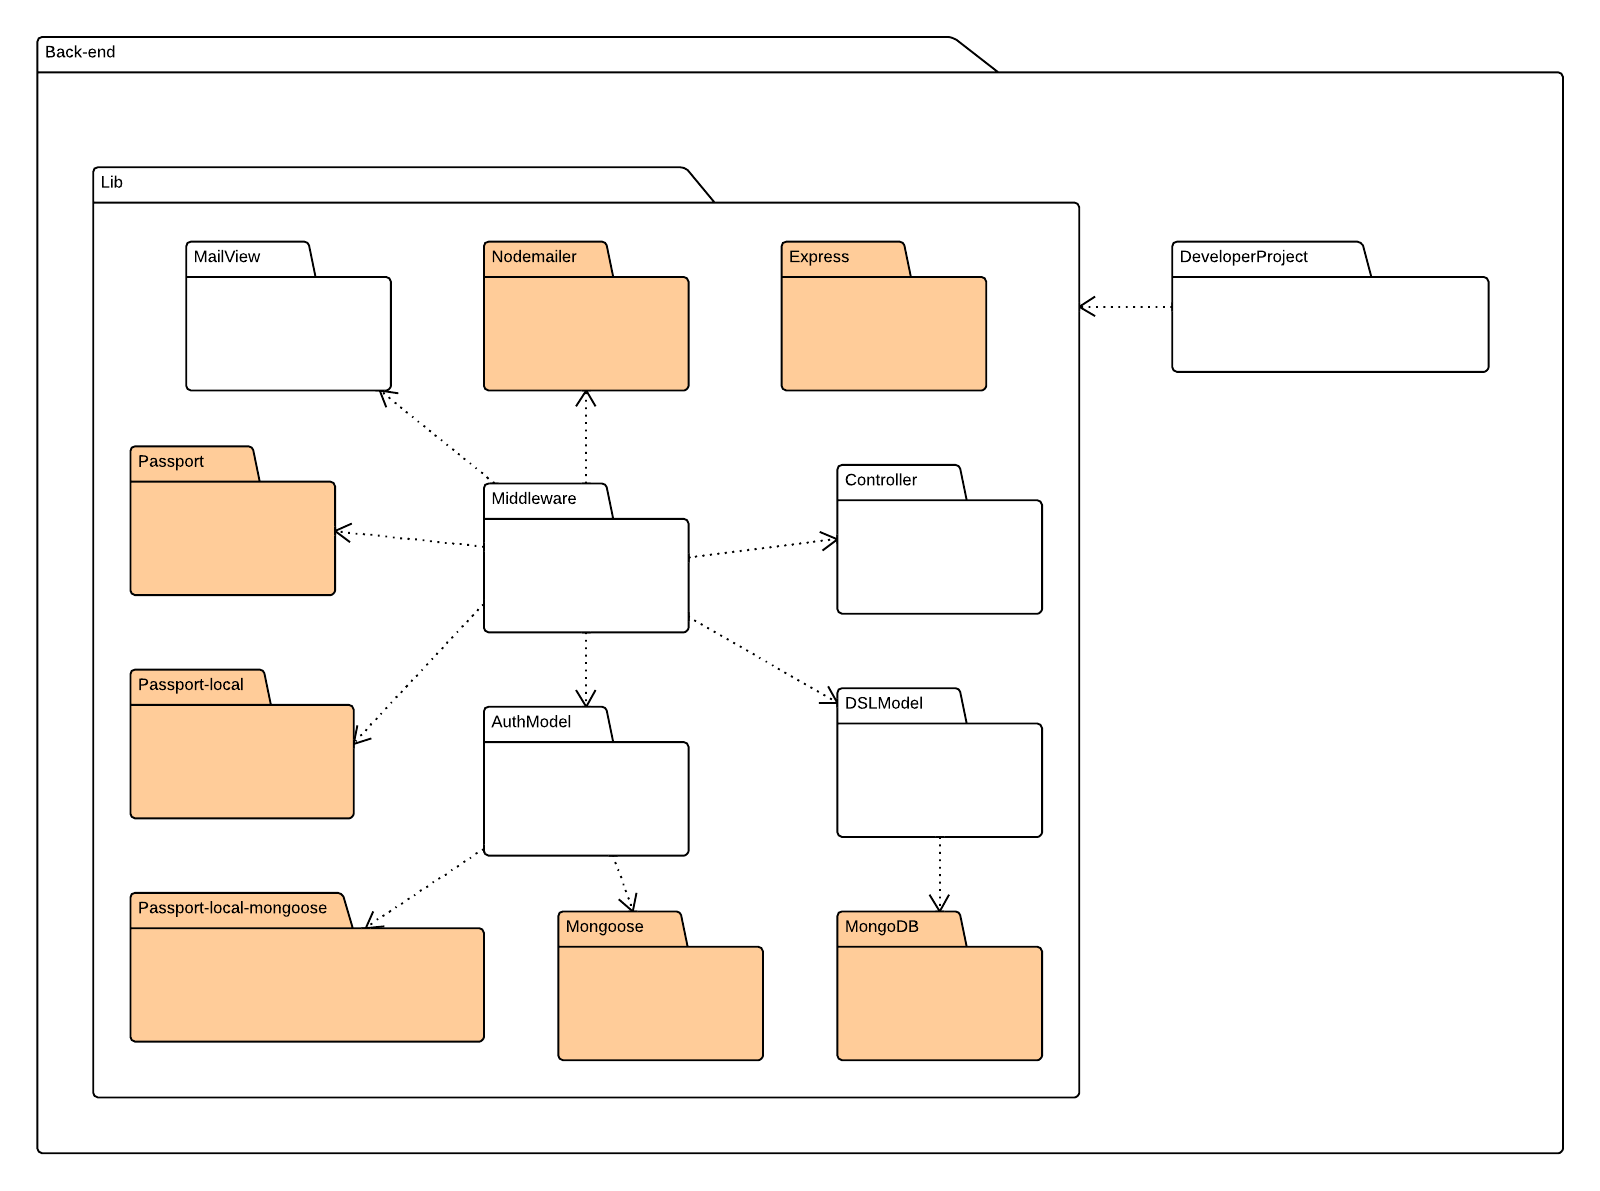
\includegraphics[width=\textwidth]{uml/Back-end-Diagramma dei Packages.png}  
        \caption{Diagramma dei packages Back-end}
      \end{center}  
    \end{figure} 
  \subparagraph{Descrizione} 
    \begin{itemize}
    \item[] \glossario{Package} che racchiude tutta la componente di \glossario{Back-end}. Comprende la libreria dell'applicazione \textit{MaaP} e il package del progetto sviluppato dal developer che andrà ad utilizzare tale libreria. \\ I packages colorati nel diagramma, rappresentano librerie esterne.
    \end{itemize} 
    \subparagraph{Package contenuti} 
    \begin{itemize}
        \item Back-end::DeveloperProject
        \item Back-end::Lib
    \end{itemize}
    
   \subparagraph{Diagramma delle classi}
    \begin{figure}[H] 
      \begin{center} 
        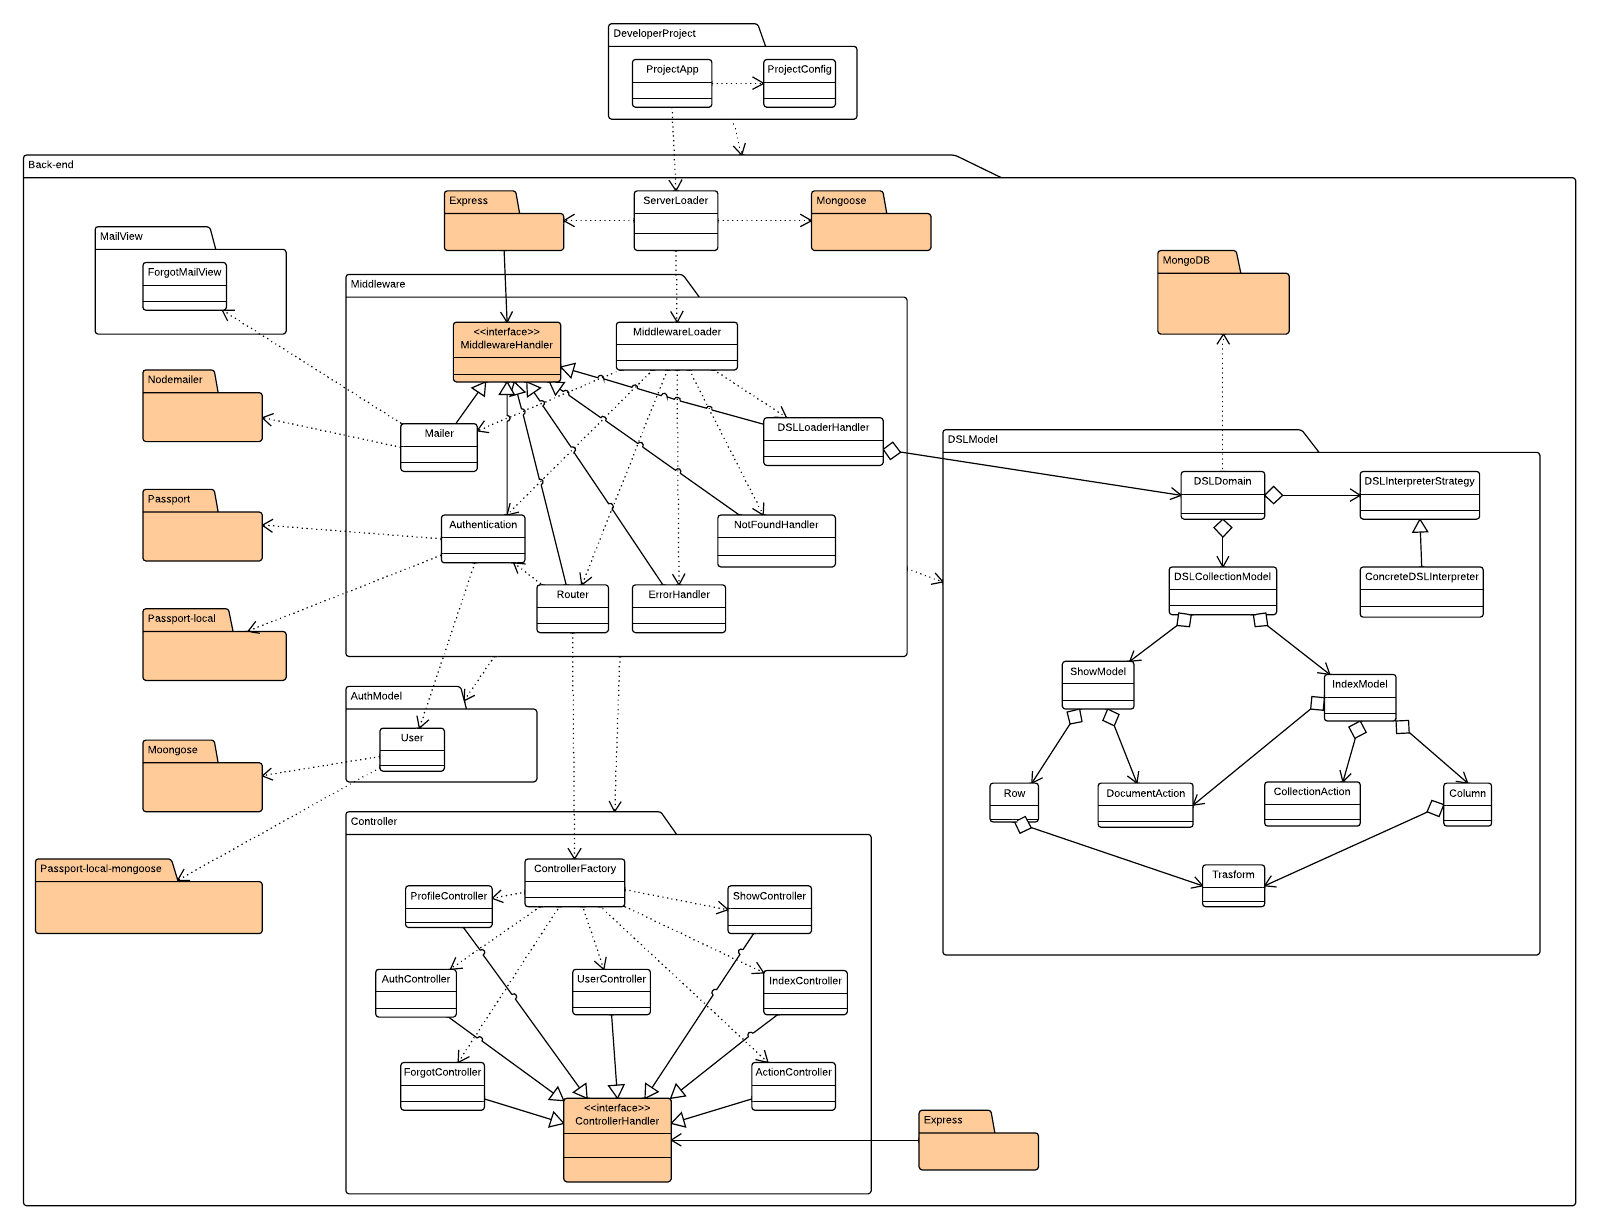
\includegraphics[width=\textwidth]{uml/Back-end-Diagramma delle classi}
        \caption{Diagramma delle classi Back-end}
      \end{center}  
    \end{figure} 
  
  \subsubsection{Back-end::Lib}
  \paragraph{Informazioni sul package} 
    \begin{figure}[H] 
      \begin{center} 
        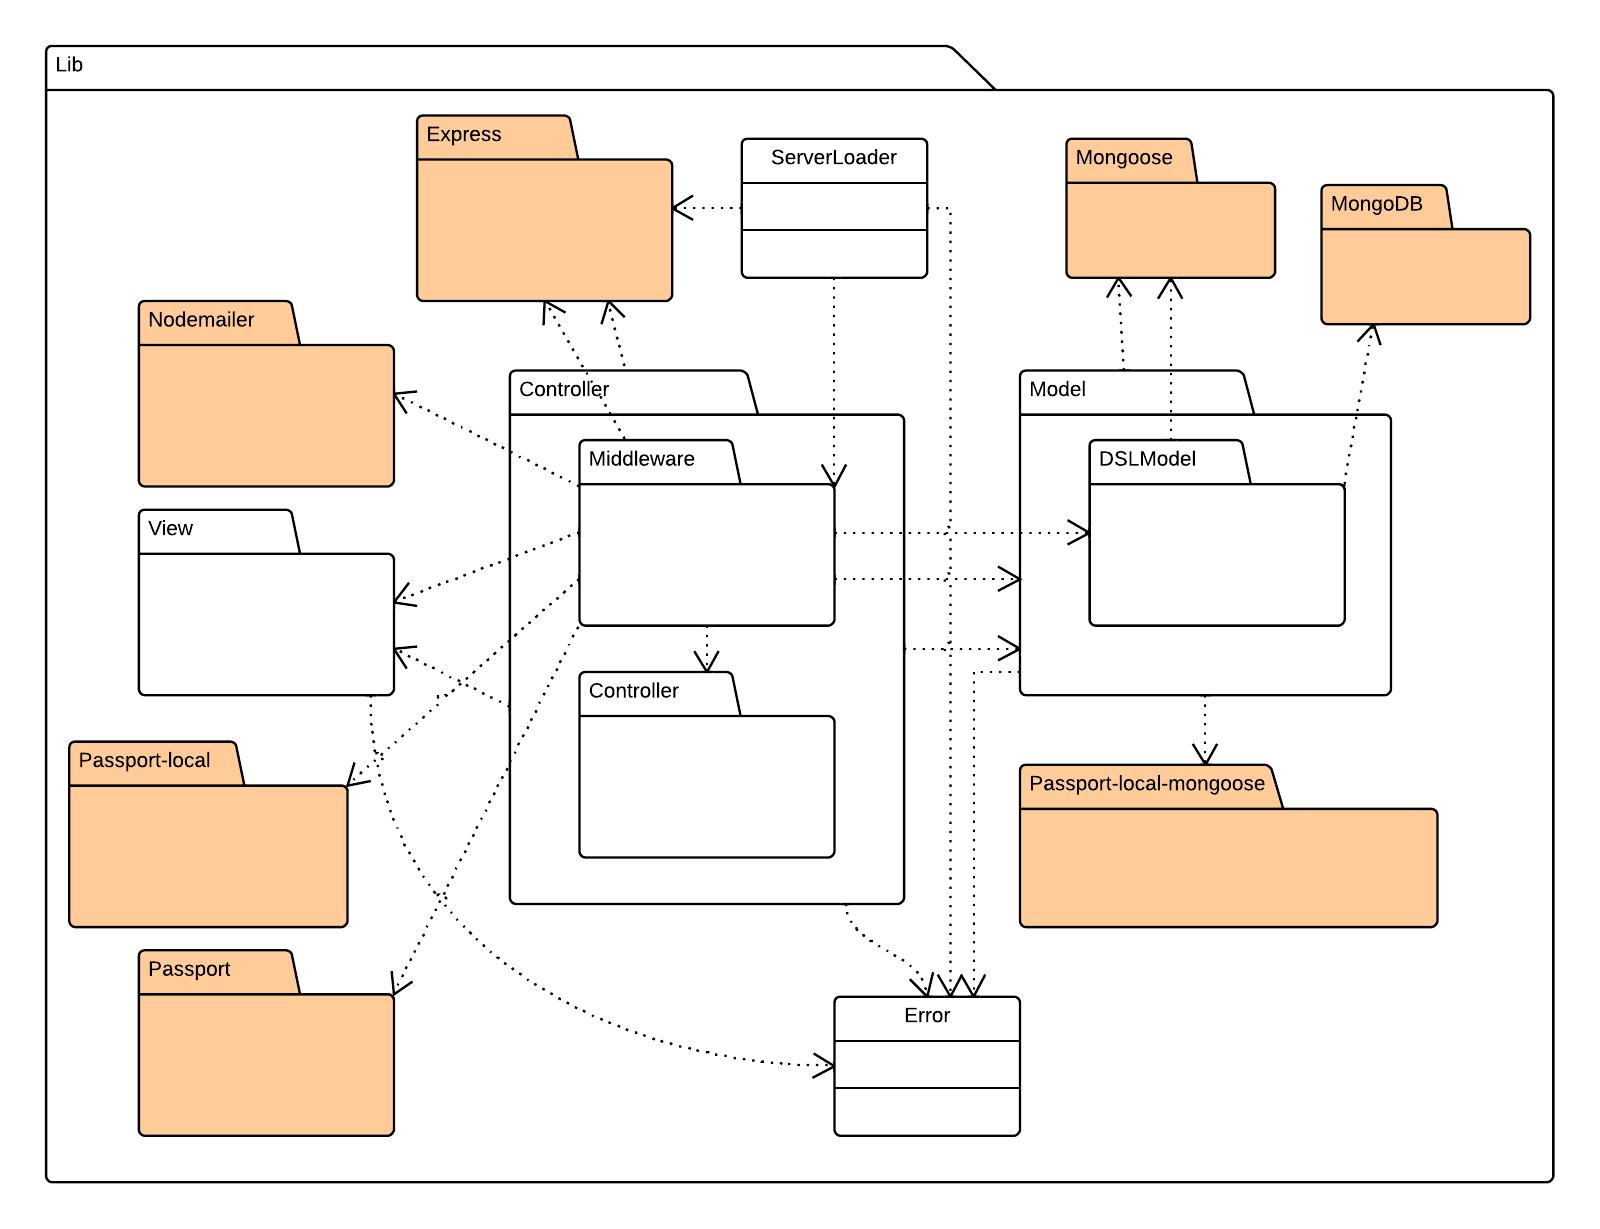
\includegraphics[width=\textwidth]{packages/Back-end::Lib.png}  
        \caption{Componente Back-end::Lib}
      \end{center}  
    \end{figure} 
  \subparagraph{Descrizione} 
    \begin{itemize}
    \item[] \glossario{Package} che costituisce la libreria principale dell'applicazione MaaP, che verrà fornita ai developer per installare e utilizzare l'applicazione. Comprende gli script per l'installazione, non rappresentati nei diagrammi in quanto non sono modellati come oggetti.
    \end{itemize} 
    \subparagraph{Package contenuti} 
    \begin{itemize}
        \item Back-end::Lib::AuthModel
        \item Back-end::Lib::DSLModel
        \item Back-end::Lib::MailView
        \item Back-end::Lib::Middleware
        \item Back-end::Lib::Controller
    \end{itemize}
    
  \subsubsection{Back-end::Lib::AuthModel}
  \paragraph{Informazioni sul package} 
    \begin{figure}[H] 
      \begin{center} 
        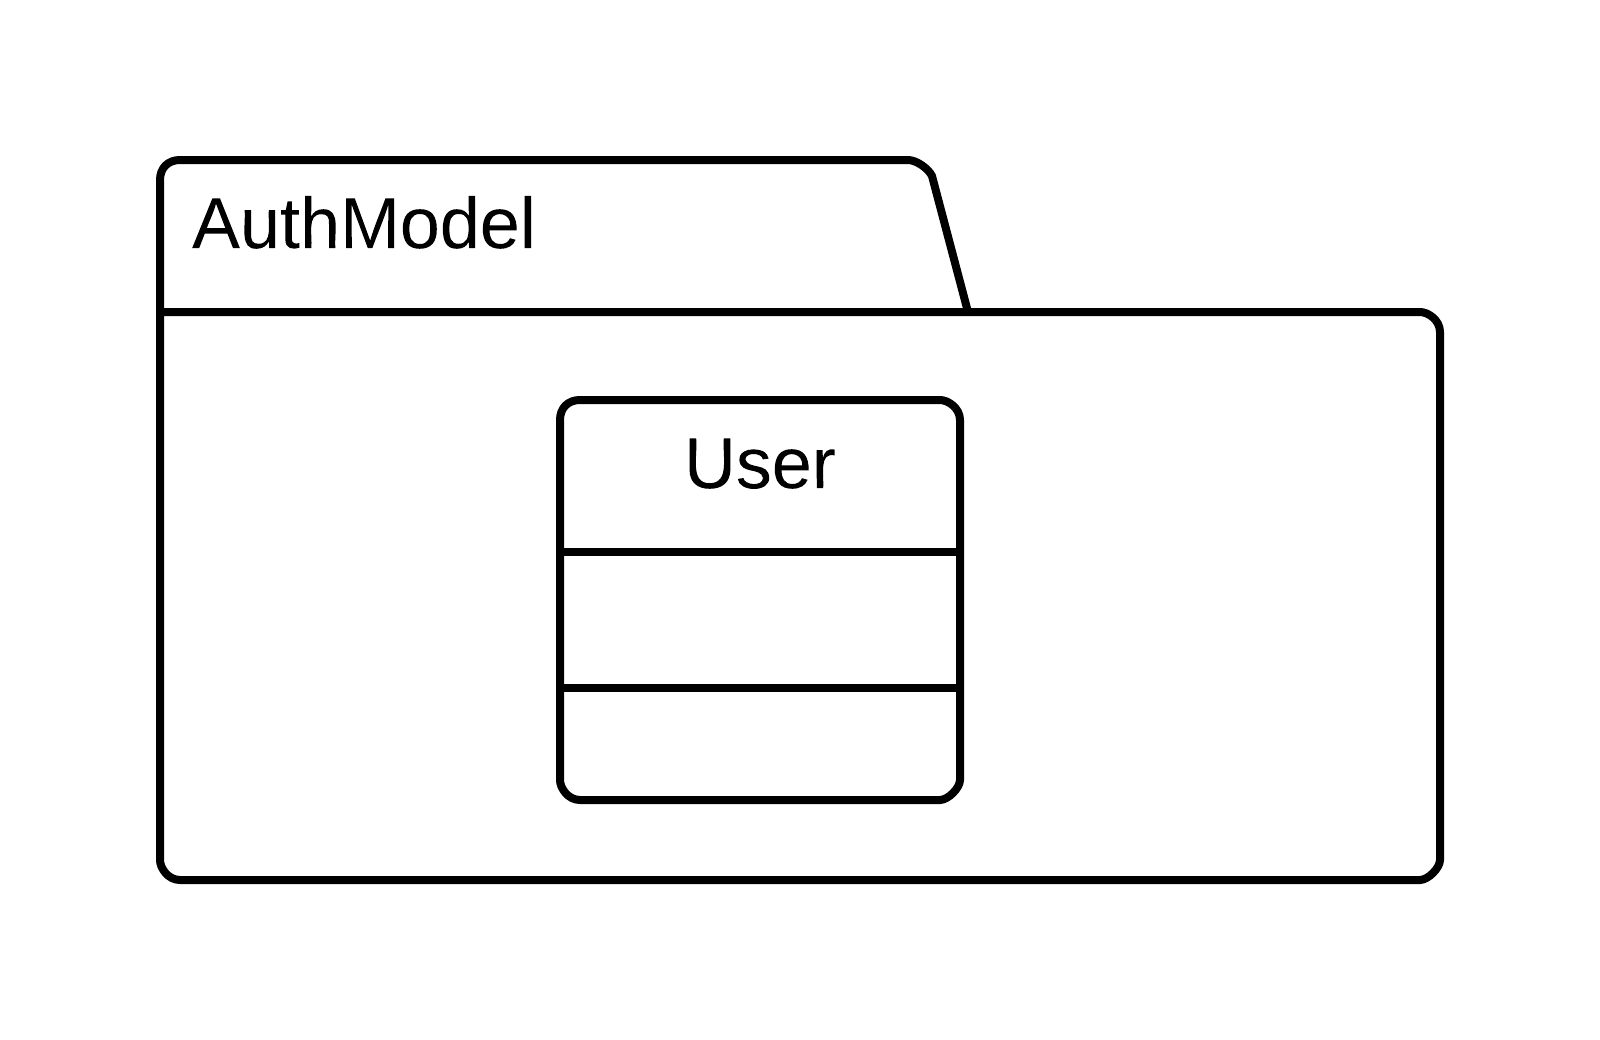
\includegraphics[width=\textwidth]{packages/Back-end::Lib::AuthModel.png}  
        \caption{Componente Back-end::Lib::AuthModel}
      \end{center}  
    \end{figure} 
  \subparagraph{Descrizione} 
    \begin{itemize}
    \item[] \glossario{Package} che gestisce i dati e le operazioni relativi all'autenticazione utente, andando ad aggiungersi alle componenti che compongono la parte model nell'architettura MVC nel back-end. 
    \end{itemize} 
    \paragraph{Classi}
      \subparagraph{Back-end::Lib::AuthModel::User}
        
        \textbf{\\ \\ Descrizione} 
          \begin{itemize}
            \item[] Classe che si occupa dei metodi per la gestione dei dati utente. 
          \end{itemize}      
        \textbf{Utilizzo}  
          \begin{itemize}
            \item[] Viene utilizzata per l'interfacciamento con la libreria \glossario{Mongoose} per la registrazione dello schema dei dati, e con la libreria passport-local-mongoose per il popolamento automatico dello schema con campi dati e metodi predefiniti.
Il costruttore del modello dello schema dei dati viene registrato nella \glossario{Factory} di \glossario{Mongoose} ed ogni istanza condividerà la stessa connessione al server.
          \end{itemize}
  \subsubsection{Back-end::DeveloperProject}
  \paragraph{Informazioni sul package} 
    \begin{figure}[H] 
      \begin{center} 
        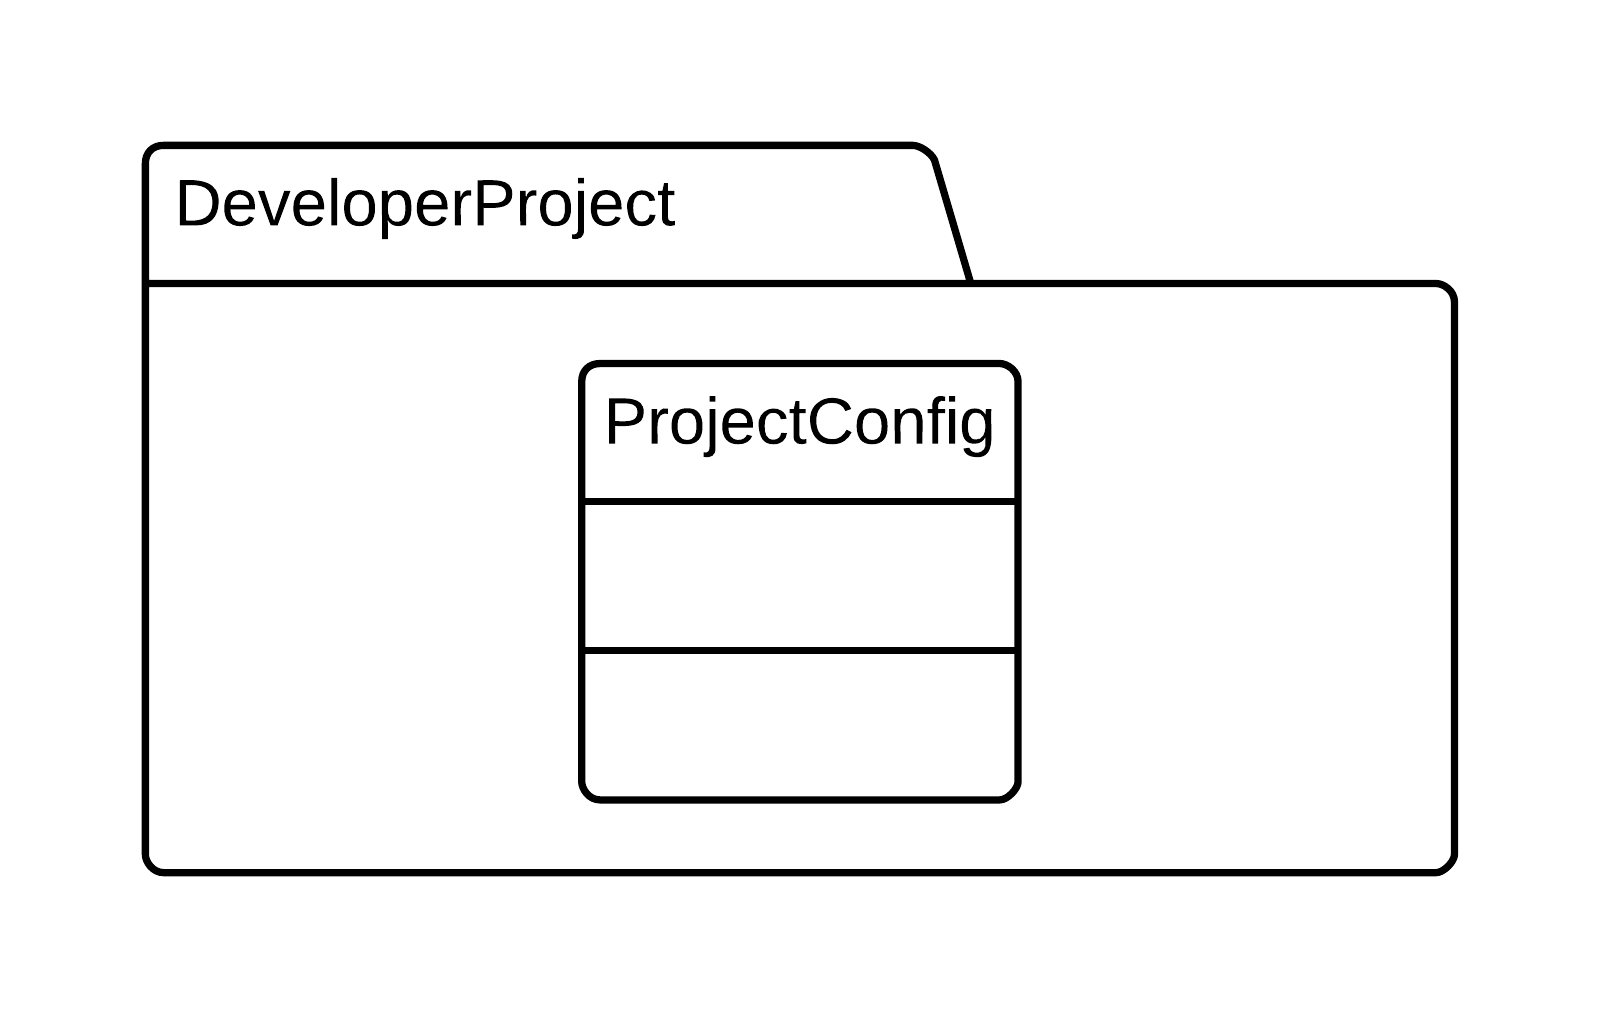
\includegraphics[width=\textwidth]{packages/Back-end::DeveloperProject.png}  
        \caption{Componente Back-end::DeveloperProject}
      \end{center}  
    \end{figure} 
  \subparagraph{Descrizione} 
    \begin{itemize}
    \item[] Questo \glossario{Package} ha il compito di fornire la configurazione e avviare il web server di \glossario{MaaP}. Consiste negli oggetti che dovranno essere predisposti dal developer che vorrà installare il framework \glossario{MaaP}. L'installazione dell framework \glossario{MaaP} fornisce uno \glossario{scaffhold} dei file e delle classi necessarie per il funzionamento dell'applicazione. Sarà compito del developer modificare tali file inserendo i dati corretti.
    \end{itemize} 
    \paragraph{Classi}
      \subparagraph{Back-end::DeveloperProject::ProjectConfig}
        
        \textbf{\\ \\ Descrizione} 
          \begin{itemize}
            \item[] Classe che si occupa di configurare il progetto creato dallo sviluppatore.
          \end{itemize}      
        \textbf{Utilizzo}  
          \begin{itemize}
            \item[] Viene utilizzata per descrivere tutti i parametri dell'applicazione. Quando viene creata una \texttt{Back-end::Lib::ServerApp} le viene passato un oggetto di questo tipo ed essa avvierà l'applicazione a partire da questa configurazione.
          \end{itemize}
  \subsubsection{Back-end::Lib::DSLModel}
  \paragraph{Informazioni sul package} 
    \begin{figure}[H] 
      \begin{center} 
        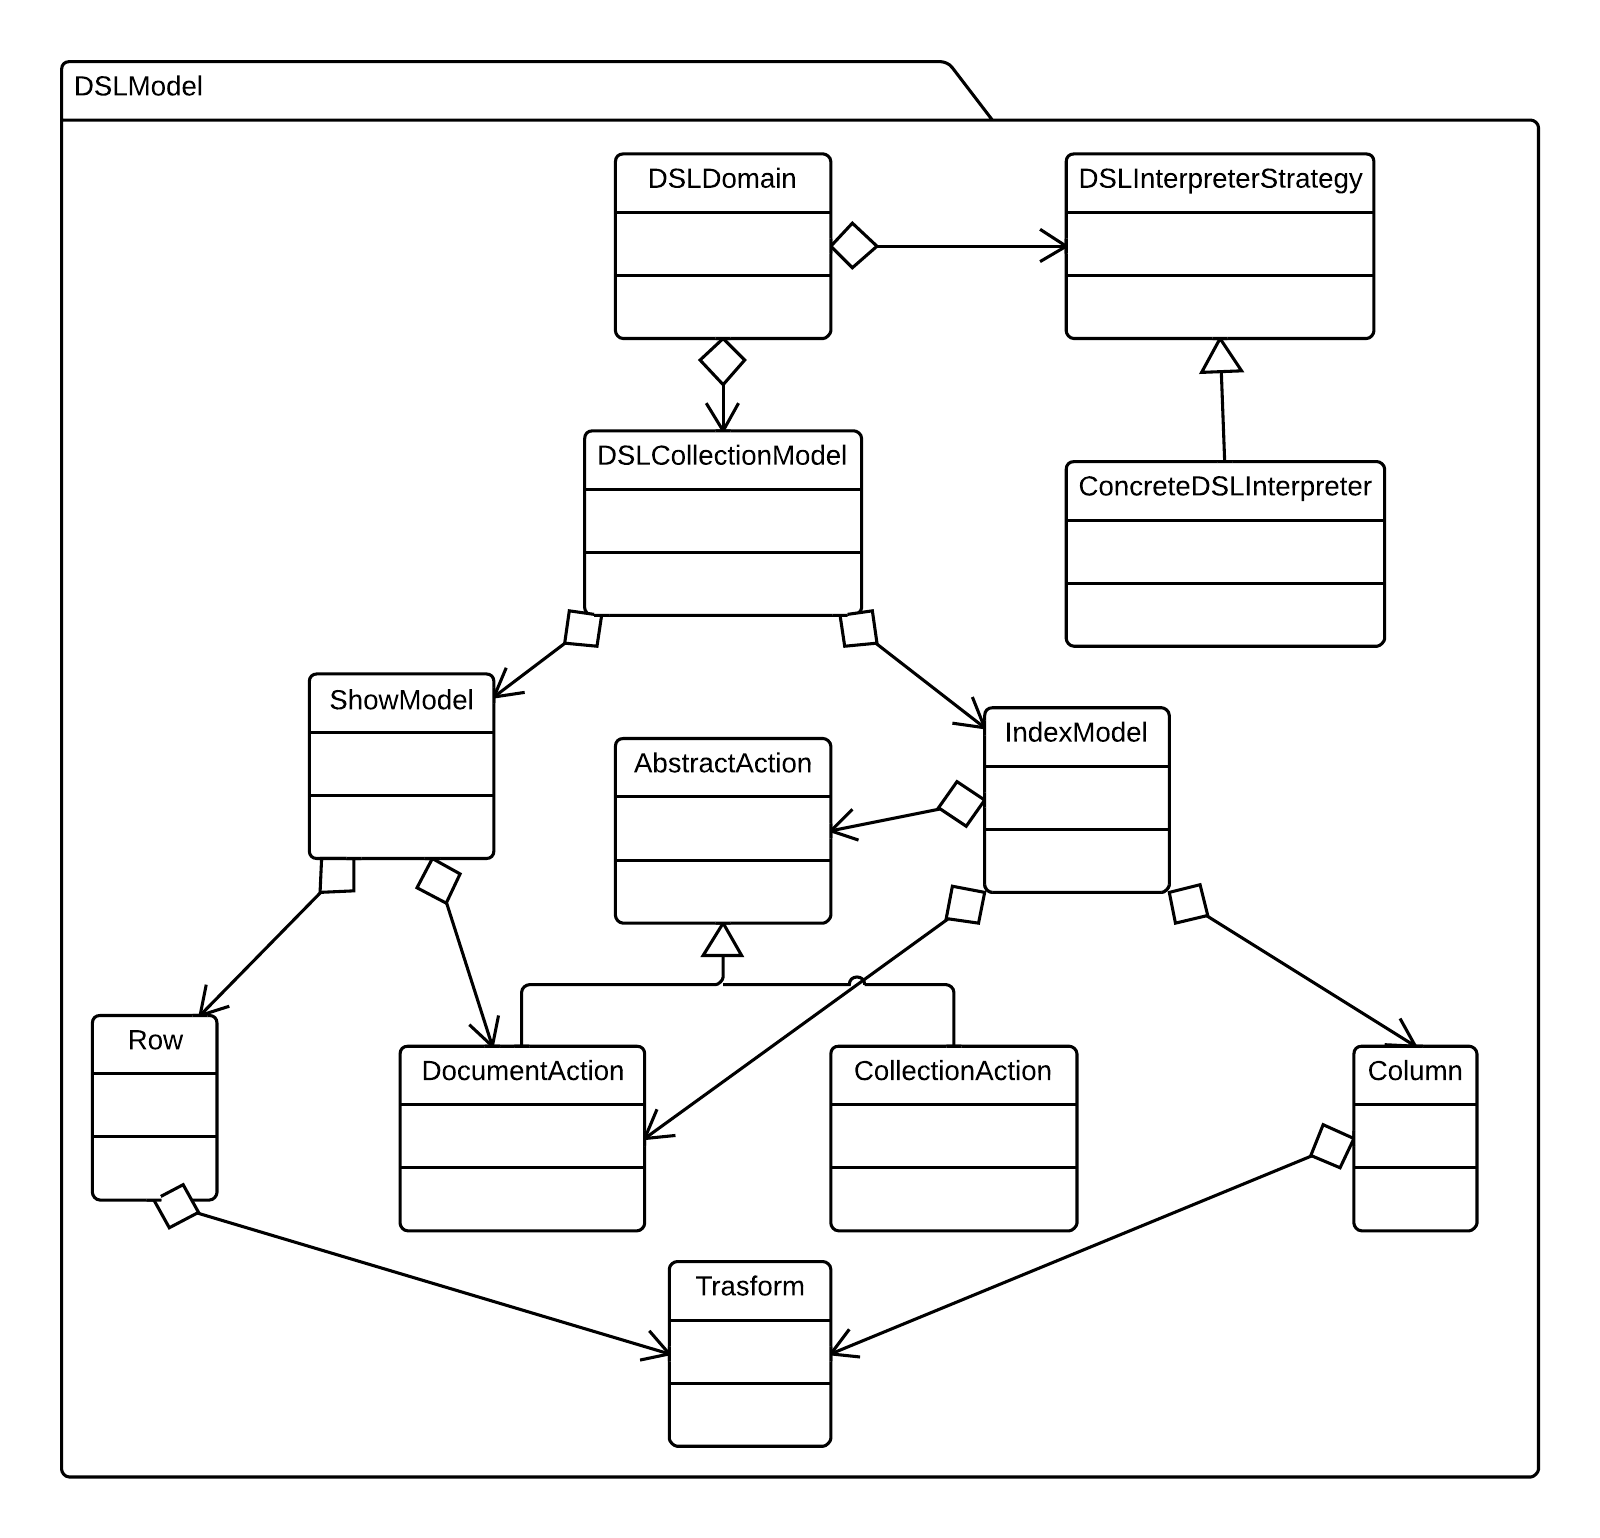
\includegraphics[width=\textwidth]{packages/Back-end::Lib::DSLModel.png}  
        \caption{Componente Back-end::Lib::DSLModel}
      \end{center}  
    \end{figure} 
  \subparagraph{Descrizione} 
    \begin{itemize}
    \item[] \glossario{Package} costituito da classi per la definizione delle regole di business sui dati definite tramite il \glossario{DSL}. 
Il \glossario{package} contiene principalmente classi che si occupano del caricamento del \glossario{DSL} e della sua rappresentazione in un modello ad oggetti. \\
Costituisce la componente model dell'architettura MVC del back-end.
    \end{itemize} 
    \paragraph{Classi}
      \subparagraph{Back-end::Lib::DSLModel::Row}
        
        \textbf{\\ \\ Descrizione} 
          \begin{itemize}
            \item[] Classe che racchiude tutte le informazioni relative ad un elemento (una riga) della show-page. Tali informazioni vengono dichiarate dal developer nel DSL.
          \end{itemize}      
        \textbf{Utilizzo}  
          \begin{itemize}
            \item[] Questa classe viene creata dalla componente che si occupa di caricare il DSL (interpretandolo o facendone il parsing). 
          \end{itemize}
      \subparagraph{Back-end::Lib::DSLModel::AbstractAction}
        
        \textbf{\\ \\ Descrizione} 
          \begin{itemize}
            \item[] Questa classe è una classe astratta che rappresenta le azione definibili dal developer nel DSL, e che potranno essere azionata tramite le \glossario{API} del \glossario{Back-end} per essere eseguite lato-server.
          \end{itemize}      
        \textbf{Utilizzo}  
          \begin{itemize}
            \item[] Questa classe viene utilizzata per raggruppare elementi comuni alle classi DocumentAction e CollectionAction.
          \end{itemize}
          \textbf{Classi Figlie}
          \begin{itemize}
              \item{Back-end::Lib::DSLModel::AbstractAction::CollectionAction}
              \item{Back-end::Lib::DSLModel::AbstractAction::DocumentAction}
          \end{itemize}
      \subparagraph{Back-end::Lib::DSLModel::DSLDomain}
        
        \textbf{\\ \\ Descrizione} 
          \begin{itemize}
            \item[] Classe che si occupa di caricare i file \glossario{DSL}. Implementa il \glossario{Design Pattern} \glossario{registry}.
          \end{itemize}      
        \textbf{Utilizzo}  
          \begin{itemize}
            \item[] Viene utilizzata per caricare dinamicamente tutti i \glossario{DSL} a partire dal \glossario{database} che le viene passato.
          \end{itemize}
          \textbf{Relazioni con altre classi}
          \begin{itemize}
              \item{Back-end::Lib::DSLModel::DSLInterpreterStrategy}
              \item{Back-end::Lib::DSLModel::DSLCollectionModel}
          \end{itemize}
      \subparagraph{Back-end::Lib::DSLModel::DSLInterpreterStrategy}
        
        \textbf{\\ \\ Descrizione} 
          \begin{itemize}
            \item[] Classe astratta che definisce l'interfaccia dell'algoritmo di interpretazione del linguaggio \glossario{DSL} utilizzato. È il componente strategy del \glossario{Design Pattern} \glossario{strategy}.
          \end{itemize}      
        \textbf{Utilizzo}  
          \begin{itemize}
            \item[] Viene utilizzata per incapsulare e rendere intercambiabile l'algoritmo di interpretazione del linguaggio \glossario{DSL}. In questo modo, se in futuro vi fosse necessità di cambiare l'algoritmo di interpretazione l'algoritmo può variare indipendentemente dal client che ne farà uso.
          \end{itemize}
          \textbf{Classi Figlie}
          \begin{itemize}
              \item{Back-end::Lib::DSLModel::DSLInterpreterStrategy::ConcreteDSLInterpreter}
          \end{itemize}
      \subparagraph{Back-end::Lib::DSLModel::DSLCollectionModel}
        
        \textbf{\\ \\ Descrizione} 
          \begin{itemize}
            \item[] Classe che si occupa di definire il model della \glossario{Collection} a partire dal \glossario{DSL}. Si ispira all'\glossario{Abstract Syntax Tree}.
          \end{itemize}      
        \textbf{Utilizzo}  
          \begin{itemize}
            \item[] È l'oggetto risultante dell'interpretazione del \glossario{DSL}. Definisce una rappresentazione interna di una \glossario{Collection}.
          \end{itemize}
          \textbf{Relazioni con altre classi}
          \begin{itemize}
              \item{Back-end::Lib::DSLModel::IndexModel}
              \item{Back-end::Lib::DSLModel::ShowModel}
          \end{itemize}
      \subparagraph{Back-end::Lib::DSLModel::DSLInterpreterStrategy::ConcreteDSLInterpreter}
        
        \textbf{\\ \\ Descrizione} 
          \begin{itemize}
            \item[] Classe che concretizza l'interprete del \glossario{DSL}. È uno dei componenti ConcreteStrategy del \glossario{Design Pattern} \glossario{Strategy}.
          \end{itemize}      
        \textbf{Utilizzo}  
          \begin{itemize}
            \item[] Viene utilizzata per implementare l'algoritmo utilizzato nell'interfaccia \texttt{Back-end::Lib::DSLModel::DSLInterpreterStrategy} per l'interpretazione del linguaggio \glossario{DSL}. Conterrà al suo interno un metodo che genererà il \glossario{parser} a partire da una grammatica regolare.
          \end{itemize}
          \textbf{Classi Ereditate}
          \begin{itemize}
                \item{Back-end::Lib::DSLModel::DSLInterpreterStrategy}
          \end{itemize}
      \subparagraph{Back-end::Lib::DSLModel::IndexModel}
        
        \textbf{\\ \\ Descrizione} 
          \begin{itemize}
            \item[] Classe che racchiude tutte le informazioni relative ad una index-page. Tali informazioni vengono dichiarate dal developer nel DSL. Comprende a sua volta altre classi di tipo Column, DocumentAction e CollectionAction.
          \end{itemize}      
        \textbf{Utilizzo}  
          \begin{itemize}
            \item[] Questa classe viene creata dalla componente che si occupa di caricare il DSL (interpretandolo o facendone il parsing).
          \end{itemize}
          \textbf{Relazioni con altre classi}
          \begin{itemize}
              \item{Back-end::Lib::DSLModel::AbstractAction::CollectionAction}
              \item{Back-end::Lib::DSLModel::AbstractAction::DocumentAction}
          \end{itemize}
      \subparagraph{Back-end::Lib::DSLModel::ShowModel}
        
        \textbf{\\ \\ Descrizione} 
          \begin{itemize}
            \item[] Classe che racchiude tutte le informazioni relative ad una show-page. 
Tali informazioni vengono dichiarate dal developer nel DSL. 
Comprende a sua volta altre classi di tipo Row e DocumentAction.
          \end{itemize}      
        \textbf{Utilizzo}  
          \begin{itemize}
            \item[] Questa classe viene creata dalla componente che si occupa di caricare il DSL (interpretandolo o facendone il parsing).
          \end{itemize}
          \textbf{Relazioni con altre classi}
          \begin{itemize}
              \item{Back-end::Lib::DSLModel::Row}
          \end{itemize}
      \subparagraph{Back-end::Lib::DSLModel::Trasform}
        
        \textbf{\\ \\ Descrizione} 
          \begin{itemize}
            \item[] Classe che racchiude tutte le informazioni relative alla modalità con cui i dati prelevati dal database verranno modificati prima di essere inviati al front-end.
Tali trasformazioni vengono dichiarate dal developer nel DSL.
          \end{itemize}      
        \textbf{Utilizzo}  
          \begin{itemize}
            \item[] Questa classe viene creata dalla componente che si occupa di caricare il DSL (interpretandolo o facendone il parsing).
          \end{itemize}
      \subparagraph{Back-end::Lib::DSLModel::Column}
        
        \textbf{\\ \\ Descrizione} 
          \begin{itemize}
            \item[] Classe che racchiude tutte le informazioni relative ad una riga della show-page. Tali informazioni vengono dichiarate dal developer nel DSL.


          \end{itemize}      
        \textbf{Utilizzo}  
          \begin{itemize}
            \item[] Questa classe viene creata dalla componente che si occupa di caricare il DSL (interpretandolo o facendone il parsing).
          \end{itemize}
          \textbf{Relazioni con altre classi}
          \begin{itemize}
              \item{Back-end::Lib::DSLModel::Trasform}
          \end{itemize}
      \subparagraph{Back-end::Lib::DSLModel::AbstractAction::CollectionAction}
        
        \textbf{\\ \\ Descrizione} 
          \begin{itemize}
            \item[] Questa classe descrive un azione definita dal developer nel DSL, che potrà essere azionata tramite le \glossario{API} del \glossario{Back-end} ed eseguita lato-server. Tale azione potrà eseguire operazioni sulla collection corrispondente al DSLCollectionModel che contiene indirettamente questa classe. La classe assume il ruolo di Command descritto dal \glossario{design pattern} Command. Gli oggetti che avranno il ruolo di ConcreteCommand verranno creati dinamicamente, definendo a run-time dei metodi aggiuntivi per questa classe.
          \end{itemize}      
        \textbf{Utilizzo}  
          \begin{itemize}
            \item[] Questa classe viene creata dalla componente che si occupa di caricare il DSL (interpretandolo o facendone il parsing).
          \end{itemize}
          \textbf{Classi Ereditate}
          \begin{itemize}
                \item{Back-end::Lib::DSLModel::AbstractAction}
          \end{itemize}
      \subparagraph{Back-end::Lib::DSLModel::AbstractAction::DocumentAction}
        
        \textbf{\\ \\ Descrizione} 
          \begin{itemize}
            \item[] Questa classe descrive un azione definita dal developer nel DSL, che potrà essere azionata tramite le \glossario{API} del \glossario{Back-end} ed eseguita lato-server. Tale azione potrà eseguire operazioni su un document della collection corrispondente al DSLCollectionModel che contiene indirettamente questa classe. La classe assume il ruolo di Command descritto dal \glossario{design pattern} Command. Gli oggetti che avranno il ruolo di ConcreteCommand verranno creati dinamicamente, definendo a run-time dei metodi aggiuntivi per questa classe.
          \end{itemize}      
        \textbf{Utilizzo}  
          \begin{itemize}
            \item[] Questa classe viene creata dalla componente che si occupa di caricare il DSL (interpretandolo o facendone il parsing). 
          \end{itemize}
          \textbf{Classi Ereditate}
          \begin{itemize}
                \item{Back-end::Lib::DSLModel::AbstractAction}
          \end{itemize}
  
  \subsubsection{Back-end::Lib::MailView}
  \paragraph{Informazioni sul package} 
    \begin{figure}[H] 
      \begin{center} 
        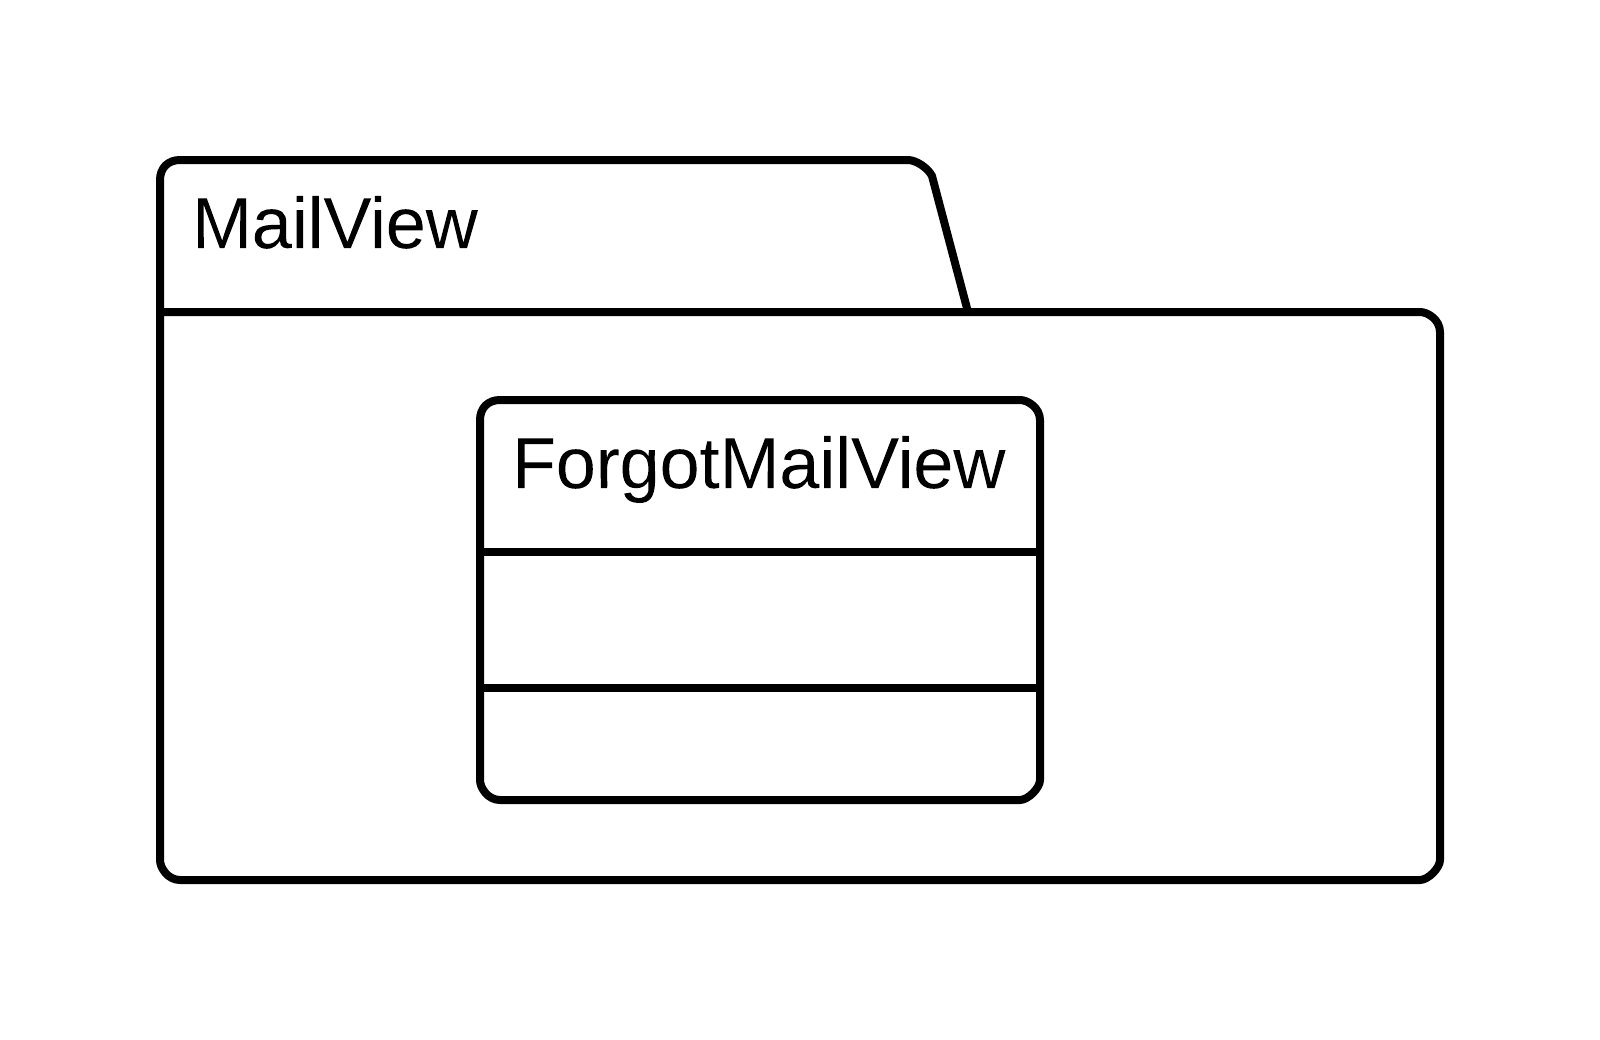
\includegraphics[width=\textwidth]{packages/Back-end::Lib::MailView.png}  
        \caption{Componente Back-end::Lib::MailView}
      \end{center}  
    \end{figure} 
  \subparagraph{Descrizione} 
    \begin{itemize}
    \item[] \glossario{Package} contenente le classi che costituiscono i template utilizzati per le email di recupero-password. Verranno utilizzate dal \glossario{middleware} Mailer.
    \end{itemize} 
    \paragraph{Classi}
      \subparagraph{Back-end::Lib::MailView::ForgotMailView}
        
        \textbf{\\ \\ Descrizione} 
          \begin{itemize}
            \item[] Classe che fornisce una rappresentazione della mail.
          \end{itemize}      
        \textbf{Utilizzo}  
          \begin{itemize}
            \item[] Viene utilizzata come template di email da inviare nel caso in cui l'utente richieda il recupero password.
          \end{itemize}
  \subsubsection{Back-end::Lib::Middleware}
  \paragraph{Informazioni sul package} 
    \begin{figure}[H] 
      \begin{center} 
        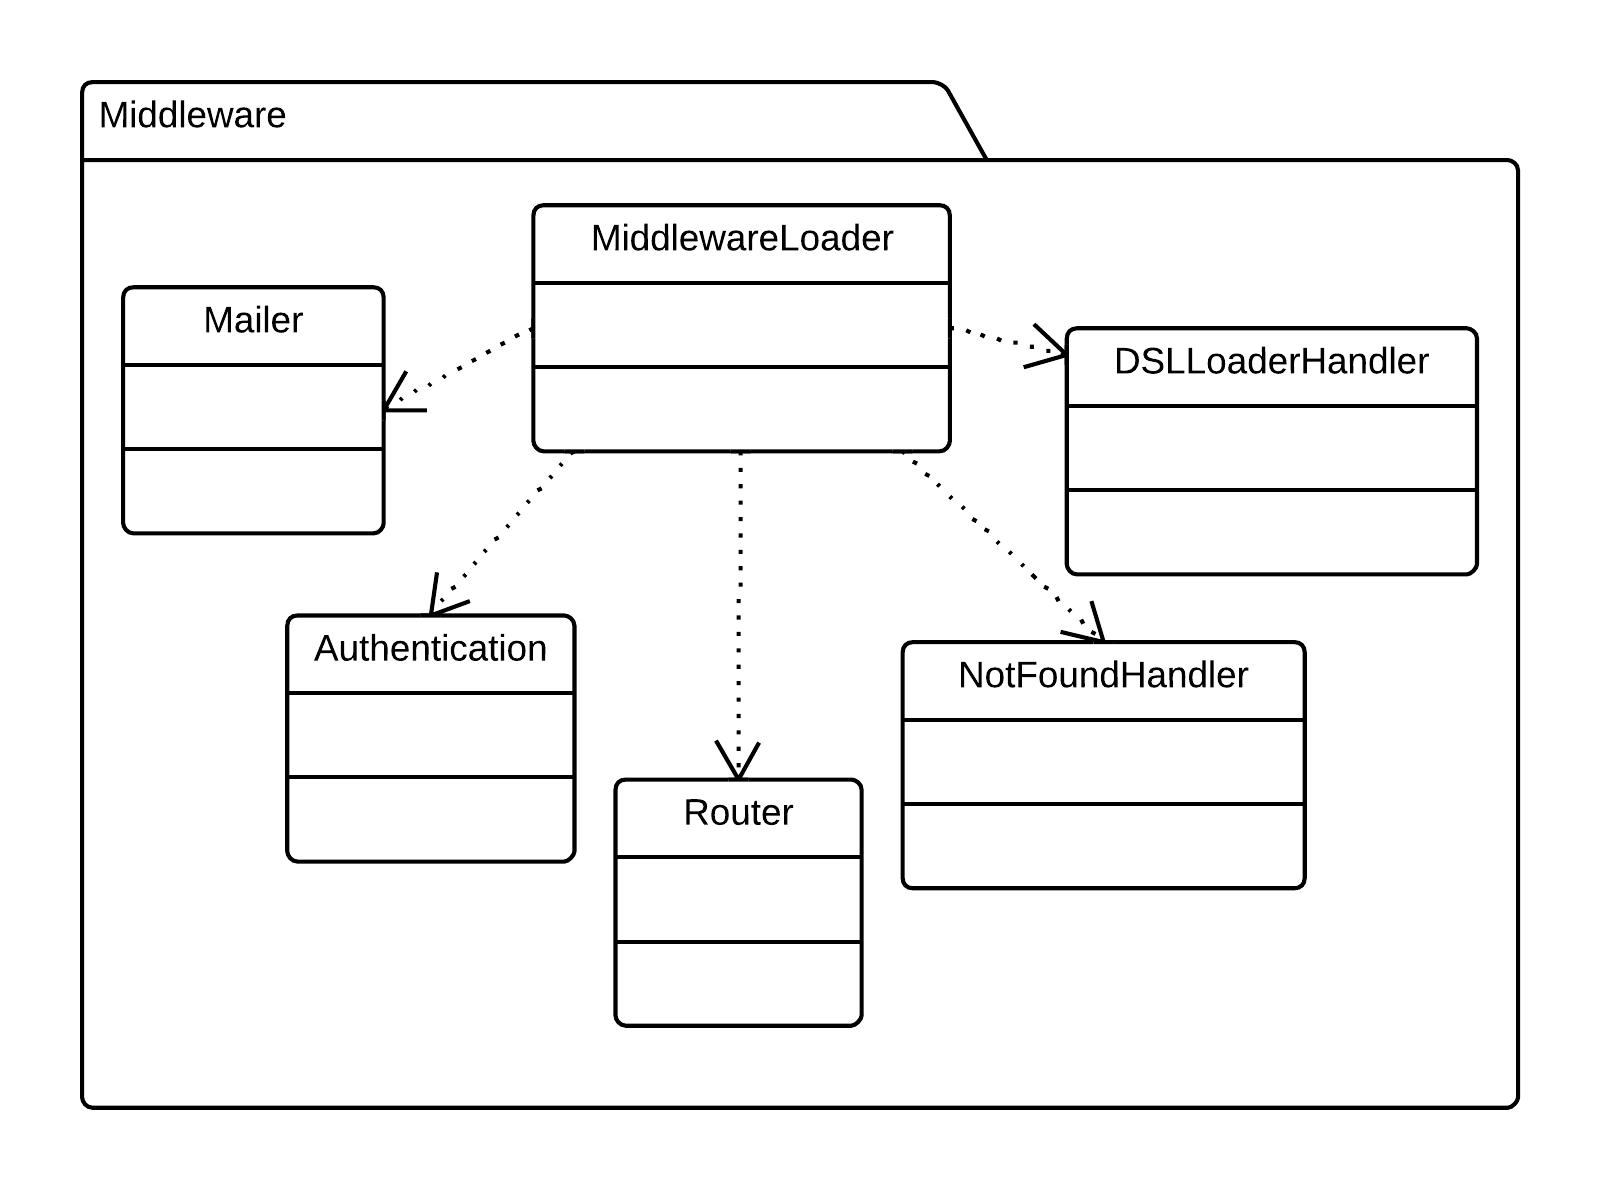
\includegraphics[width=\textwidth]{packages/Back-end::Lib::Middleware.png}  
        \caption{Componente Back-end::Lib::Middleware}
      \end{center}  
    \end{figure} 
  \subparagraph{Descrizione} 
    \begin{itemize}
    \item[] \glossario{Package} contenente classi che costituiscono gli handler della catena di chiamate a cui viene passata la responsabilità di gestire una richiesta,  decorando quest'ultima con parametri e metodi utilizzabili dai controller. Costituisce una parte dell' \glossario{application logic} nell'architettura \glossario{MVC} del \glossario{Back-end}.
    \end{itemize} 
    \paragraph{Classi}
      \subparagraph{Back-end::Lib::Middleware::Router}
        
        \textbf{\\ \\ Descrizione} 
          \begin{itemize}
            \item[] Classe che si occupa della richiesta di risorse. È uno dei componenti subsystem class del \glossario{Design Pattern} \glossario{Facade} e handler del \glossario{Design Pattern} \glossario{Chain of responsability}.
          \end{itemize}      
        \textbf{Utilizzo}  
          \begin{itemize}
            \item[] Si occupa di smistare la richiesta in base all'\glossario{URI} ricevuto e ad invocare l'opportuno metodo di creazione sulla classe \texttt{Back-end::Lib::Controller::ControllerFactory}.
          \end{itemize}
      \subparagraph{Back-end::Lib::Middleware::Authentication}
        
        \textbf{\\ \\ Descrizione} 
          \begin{itemize}
            \item[] Classe che si occupa dell'autenticazione di un'utente. È uno dei componenti subsystem class del \glossario{Design Pattern} \glossario{Facade} e handler del \glossario{Design Pattern} \glossario{Chain of responsability}.
          \end{itemize}      
        \textbf{Utilizzo}  
          \begin{itemize}
            \item[] Viene utilizzata per verificare i dati inseriti dall'utente nella pagina di login e controllare l'effettiva corrispondenza delle credenziali nel \glossario{database}.
          \end{itemize}
          \textbf{Relazioni con altre classi}
          \begin{itemize}
              \item{Back-end::Lib::AuthModel::User}
          \end{itemize}
      \subparagraph{Back-end::Lib::Middleware::DSLLoaderHandler}
        
        \textbf{\\ \\ Descrizione} 
          \begin{itemize}
            \item[] Classe che si occupa di caricare i \glossario{DSL} presenti nel sistema. È uno dei componenti subsystem class del \glossario{Design Pattern} \glossario{Facade} e handler del \glossario{Design Pattern} \glossario{Chain of responsability}.
          \end{itemize}      
        \textbf{Utilizzo}  
          \begin{itemize}
            \item[] Viene utilizzata per caricare i \glossario{DSL} delle \glossario{Collection} all'interno del \glossario{database}.
          \end{itemize}
          \textbf{Relazioni con altre classi}
          \begin{itemize}
              \item{Back-end::Lib::DSLModel::DSLDomain}
          \end{itemize}
      \subparagraph{Back-end::Lib::Middleware::Mailer}
        
        \textbf{\\ \\ Descrizione} 
          \begin{itemize}
            \item[] Classe che si occupa dell'invio di email. È uno dei componenti subsystem class del \glossario{Design Pattern} \glossario{Facade} e handler del \glossario{Design Pattern} \glossario{Chain of responsability}.
          \end{itemize}      
        \textbf{Utilizzo}  
          \begin{itemize}
            \item[] Viene utilizzata per inviare un'email ad un utente che ha effettuato la richiesta di recupero password.
          \end{itemize}
          \textbf{Relazioni con altre classi}
          \begin{itemize}
              \item{Back-end::Lib::MailView::ForgotMailView}
          \end{itemize}
      \subparagraph{Back-end::Lib::Middleware::MiddlewareLoader}
        
        \textbf{\\ \\ Descrizione} 
          \begin{itemize}
            \item[] Classe che definisce un'interfaccia comune per tutte le richieste dell'applicazione. È la componente facade del \glossario{Design Pattern} \glossario{Facade} e handler del \glossario{Design Pattern} \glossario{Chain of responsability}.
          \end{itemize}      
        \textbf{Utilizzo}  
          \begin{itemize}
            \item[] Viene utilizzato per istanziare in modo "nascosto" all'applicazione tutti i \glossario{middleware} presenti nel componente \texttt{Back-end::Lib::Middleware}.
          \end{itemize}
          \textbf{Relazioni con altre classi}
          \begin{itemize}
              \item{Back-end::Lib::Middleware::Router}
              \item{Back-end::Lib::Middleware::Authentication}
              \item{Back-end::Lib::Middleware::DSLLoaderHandler}
              \item{Back-end::Lib::Middleware::Mailer}
              \item{Back-end::Lib::Middleware::NotFoundHandler}
          \end{itemize}
      \subparagraph{Back-end::Lib::Middleware::NotFoundHandler}
        
        \textbf{\\ \\ Descrizione} 
          \begin{itemize}
            \item[] Classe che si occupa la gestione dell'errore di pagina non trovata. È uno dei componenti subsystem class del \glossario{Design Pattern} \glossario{Facade} e handler del \glossario{Design Pattern} \glossario{Chain of responsability}.
          \end{itemize}      
        \textbf{Utilizzo}  
          \begin{itemize}
            \item[] Viene utilizzata per generare una pagina 404 di errore nel caso in cui l'\glossario{URI} passato non corrisponda ad una risorsa presente nell'applicazione.
          \end{itemize}
      \subparagraph{Back-end::Lib::Middleware::Errorhandler}
        
        \textbf{\\ \\ Descrizione} 
          \begin{itemize}
            \item[] Questa classe gestisce gli errori generati nei precedenti middleware o controller. Invia al client una risposta con stato HTTP 500 (server error) con una descrizione dell'errore nel formato JSON.
È uno dei componenti subsystem class del \glossario{Design Pattern} \glossario{Facade} e handler del \glossario{Design Pattern} \glossario{Chain of responsability}.
          \end{itemize}      
        \textbf{Utilizzo}  
          \begin{itemize}
            \item[] Questo middleware viene utilizzato per ultimo nella catena di gestione delle richieste di Express, in modo da gestire tutti gli errori generati precedentemente.
          \end{itemize}
  \subsubsection{Back-end::Lib::Controller}
  \paragraph{Informazioni sul package} 
    \begin{figure}[H] 
      \begin{center} 
        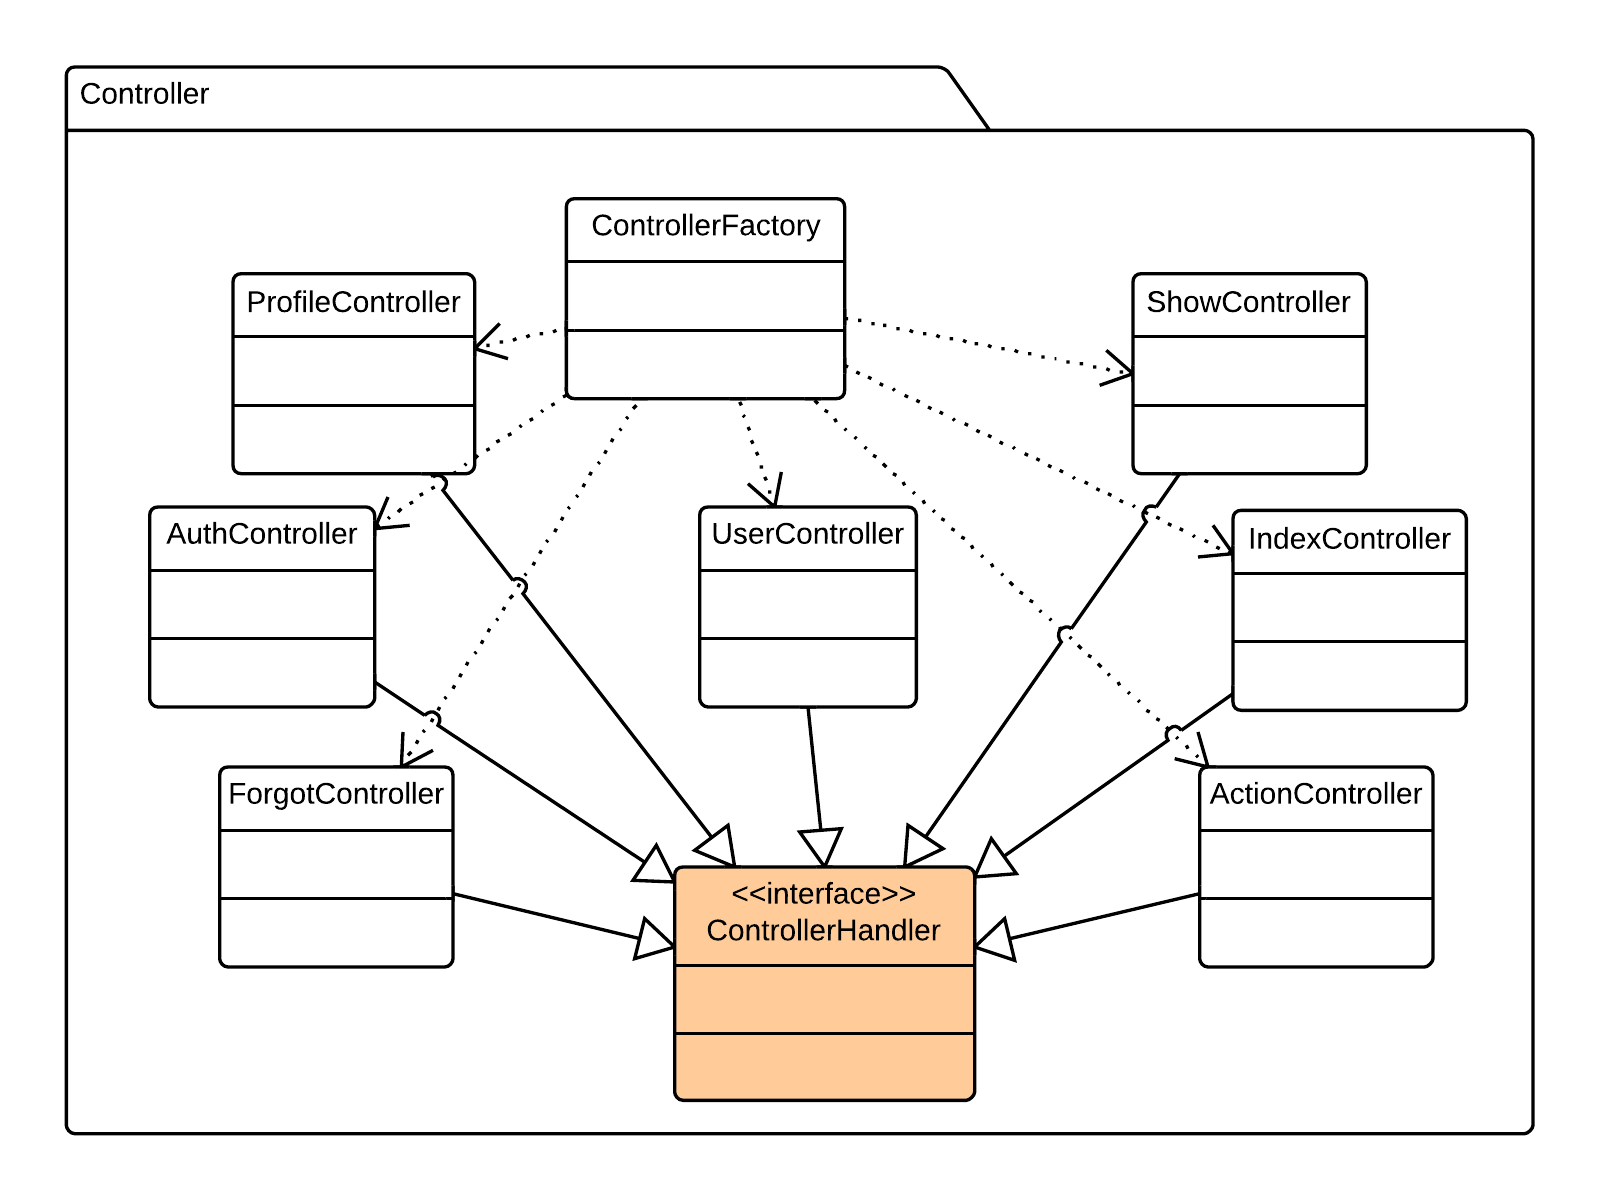
\includegraphics[width=\textwidth]{packages/Back-end::Lib::Controller.png}  
        \caption{Componente Back-end::Lib::Controller}
      \end{center}  
    \end{figure} 
  \subparagraph{Descrizione} 
    \begin{itemize}
    \item[] \glossario{Package} per il componente che realizza parte controller nell'architettura mvc nel back-end. Contiene classi per le funzionalità di controllo e visualizzazione delle risorse, dove ogni classe gestisce in modo esclusivo una sola di queste, in base all' \glossario{URI}.
    \end{itemize} 
    \paragraph{Classi}
      \subparagraph{Back-end::Lib::Controller::UserController}
        
        \textbf{\\ \\ Descrizione} 
          \begin{itemize}
            \item[] Classe che si occupa della varie operazioni che l'admin può compiere sugli utenti dell'applicazione. È uno dei componenti product del \glossario{Design Pattern} \glossario{Factory method}.
          \end{itemize}      
        \textbf{Utilizzo}  
          \begin{itemize}
            \item[] Viene utilizzata per visualizzare la \glossario{index-page} degli utenti, visualizzare le relative \glossario{show-page}, eliminare un utente e modificare il profilo. Mette a disposizione dei metodi per effettuare tutte queste operazioni.
          \end{itemize}
      \subparagraph{Back-end::Lib::Controller::ActionController}
        
        \textbf{\\ \\ Descrizione} 
          \begin{itemize}
            \item[] Classe che rappresenta i metodi per la gestione della risorsa corrispondente ad un'azione. 
È uno dei componenti product del \glossario{Design Pattern} \glossario{Factory method}.
          \end{itemize}      
        \textbf{Utilizzo}  
          \begin{itemize}
            \item[] Viene utilizzata per gestire le azioni personalizzate predisposte nelle pagine index-page e show-page, delegando alla classe \texttt{Back-end::Lib::DSLModel::DSLDomain} la loro esecuzione avendo quest'ultima l'implementazione delle stesse. 
          \end{itemize}
      \subparagraph{Back-end::Lib::Controller::ControllerFactory}
        
        \textbf{\\ \\ Descrizione} 
          \begin{itemize}
            \item[] Classe che si occupa di istanziare e restituire una classe \textit{Controller}. Rappresenta il componente creator del \glossario{Design Pattern} \glossario{Factory method}.
          \end{itemize}      
        \textbf{Utilizzo}  
          \begin{itemize}
            \item[] Viene costruita una sola volta dalla classe \texttt{Back-end::Lib::Middleware::Router} e si occupa di creare e restituire l'oggetto \textit{Controller} richiesto.
          \end{itemize}
      \subparagraph{Back-end::Lib::Controller::AuthController}
        
        \textbf{\\ \\ Descrizione} 
          \begin{itemize}
            \item[] Classe che rappresenta i metodi per la gestione delle risorse di login e logout. È uno dei componenti product del \glossario{Design Pattern} \glossario{Factory method}.

          \end{itemize}      
        \textbf{Utilizzo}  
          \begin{itemize}
            \item[] Viene utilizzata per gestire i dati di e le operazioni relativi all'autenticazione utente e al suo logout dall'applicazione, occupandosi della creazione della sessione utente e della sua distruzione tramite \glossario{cookies}.
          \end{itemize}
      \subparagraph{Back-end::Lib::Controller::ProfileController}
        
        \textbf{\\ \\ Descrizione} 
          \begin{itemize}
            \item[] Classe che rappresenta la gestione di un profilo utente. È uno dei componenti product del \glossario{Design Pattern} \glossario{Factory method}.
          \end{itemize}      
        \textbf{Utilizzo}  
          \begin{itemize}
            \item[] Viene utilizzata per visualizzare il profilo dell'utente, tramite GET, e per editarlo tramite PUT.
          \end{itemize}
      \subparagraph{Back-end::Lib::Controller::ShowController}
        
        \textbf{\\ \\ Descrizione} 
          \begin{itemize}
            \item[] Classe che si occupa della gestione della risorsa show-page.
È uno dei componenti product del \glossario{Design Pattern} \glossario{Factory method}.
          \end{itemize}      
        \textbf{Utilizzo}  
          \begin{itemize}
            \item[] Viene utilizzata per gestire una richiesta della risorsa show-page, delegando alla classe \texttt{Back-end::Lib::DSLModel::DSLDomain} la sua visualizzazione.
          \end{itemize}
      \subparagraph{Back-end::Lib::Controller::IndexController}
        
        \textbf{\\ \\ Descrizione} 
          \begin{itemize}
            \item[] Classe di gestione per la risorsa index 
È uno dei componenti product del \glossario{Design Pattern} \glossario{Factory method}.

          \end{itemize}      
        \textbf{Utilizzo}  
          \begin{itemize}
            \item[] Viene utilizzata per gestire la risorsa corrispondente all'index-page di un \glossario{Document}, offrendo metodi per restituirne gli attributi, effettuarne la modifica o la cancellazione e delega la visualizzazione dell'index-page alla classe \texttt{Back-end::Lib::DSLModel::DSLDomain}.

          \end{itemize}
      \subparagraph{Back-end::Lib::Controller::ForgotController}
        
        \textbf{\\ \\ Descrizione} 
          \begin{itemize}
            \item[] Classe che rappresenta il sistema di recupero e ripristino password. È uno dei componenti product del \glossario{Design Pattern} \glossario{Factory method}.
          \end{itemize}      
        \textbf{Utilizzo}  
          \begin{itemize}
            \item[] La classe fornisce dei metodi per effettuare una richiesta di reset password e, in un secondo momento, procedere al suo ripristino. La richiesta di reset avviene mandando un'email all'indirizzo dell'utente tramite la classe \texttt{Back-end::Lib::Middleware::Mailer}. All'interno di questo messaggio sarà presente un link che procederà ad effettuare il login dell'utente e a reindirizzarlo nella pagina di modifica profilo, dalla quale potrà modificare la password.
          \end{itemize}

\subsection{Scenari}

\subsubsection{Gestione generale delle richieste}
Nel diagramma che rappresenta lo scenario della gestione richieste viene mostrata l'iterazione tra server e middleware, alcuni dei quali sono offerti da Express, altri sono definiti dall'utente o da altre librerie. I \glossario{Middleware} si distinguono in Middleware di gestione delle richieste e Middleware di gestione degli errori, a seconda del numero di parametri con cui vengono invocati.

Segue un elenco ordinato dei middleware utilizzati. L'ordine in cui elaborano la richiesta è determinante, poiché ciascuno costituisce un handler del pattern Chain of Responsibility e ha la facoltà di interrompere la catena di chiamate.

\begin{itemize}
\item{express.compress()}: \glossario{Middleware} per comprimere  con il formato \glossario{gzip} le comunicazioni.
\item{express.logger()}: \glossario{Middleware} utilizzato per registrare un log delle richieste, utile per fare il
\glossario{debugging} dell'applicazione.
\item{express.json()}: \glossario{Middleware} che estrae dalle richiesta i parametri che sono nel formato JSON.
\item{express.urlencoded()}: \glossario{Middleware} che estrae dalle richiesta i parametri di tipo www-form-encoded, arrivati ad esempio con una richiesta POST.
\item{express.methodOverride()}: \glossario{Middleware} utilizzato per permettere anche ai vecchi browser di avere un modo per fare richieste PUT e DELETE.
\item{express.cookieParser()}: \glossario{Middleware} che analizza i \glossario{cookie}.
\item{express.cookieSession()}: \glossario{Middleware} per la gestione di sessioni utente basate su cookies.
\item{Authentication}: \glossario{Middleware} da noi scritto per gestire l'autenticazione. Utilizza nello specifico:
	\begin{itemize}
	\item{passport.initialize()}: \glossario{Middleware} utilizzato per l'inizializzazione di Passport.
	\item{passport.session()}:  \glossario{Middleware} che permette di memorizzare i record della sessione utente per mantenerne lo stato di login. 
	\end{itemize}
\item{express.router()}: \glossario{Middleware} con cui Express gestisce le richieste, smistandole a diversi controller in base alla URI e al metodo HTTP con cui sono state richieste (GET, PUT, POST, DELETE).
\item{express.static()}: \glossario{Middleware} per servire contenuti statici.
\item{NotFoundHandler}: un \glossario{Middleware} da noi scritto per gestire le richieste che non vengono gestite da nessun controller (errore client 404).
\item{ErrorHandler}: \glossario{Middleware} da noi scritto per gestire gli errori sollevati da uno dei precedenti middleware (errore server 500).
\end{itemize}

Nel seguente diagramma viene rappresentata una generica richiesta al server: utilizzando il pattern della Chain of Responsibility, il server invoca in sequenza i middleware(ad esempio i middleware Router,Gestore Errore), passando come parametri l'oggetto della richiesta, della risposta e una callback per passare il controllo al successivo middleware. In caso di errore, un middleware può chiamare la callback passandogli la descrizione dell'errore come parametro \code{next(error)}. In questo modo il server passerà il controllo al primo middleware in grado di gestire un errore. Come terza alternativa, un middleware può terminare la propria esecuzione con un \code{return}. In tal caso la richiesta non verrà più gestita da nessun altro middleware.

\begin{figure}[H]
	\begin{center} 
		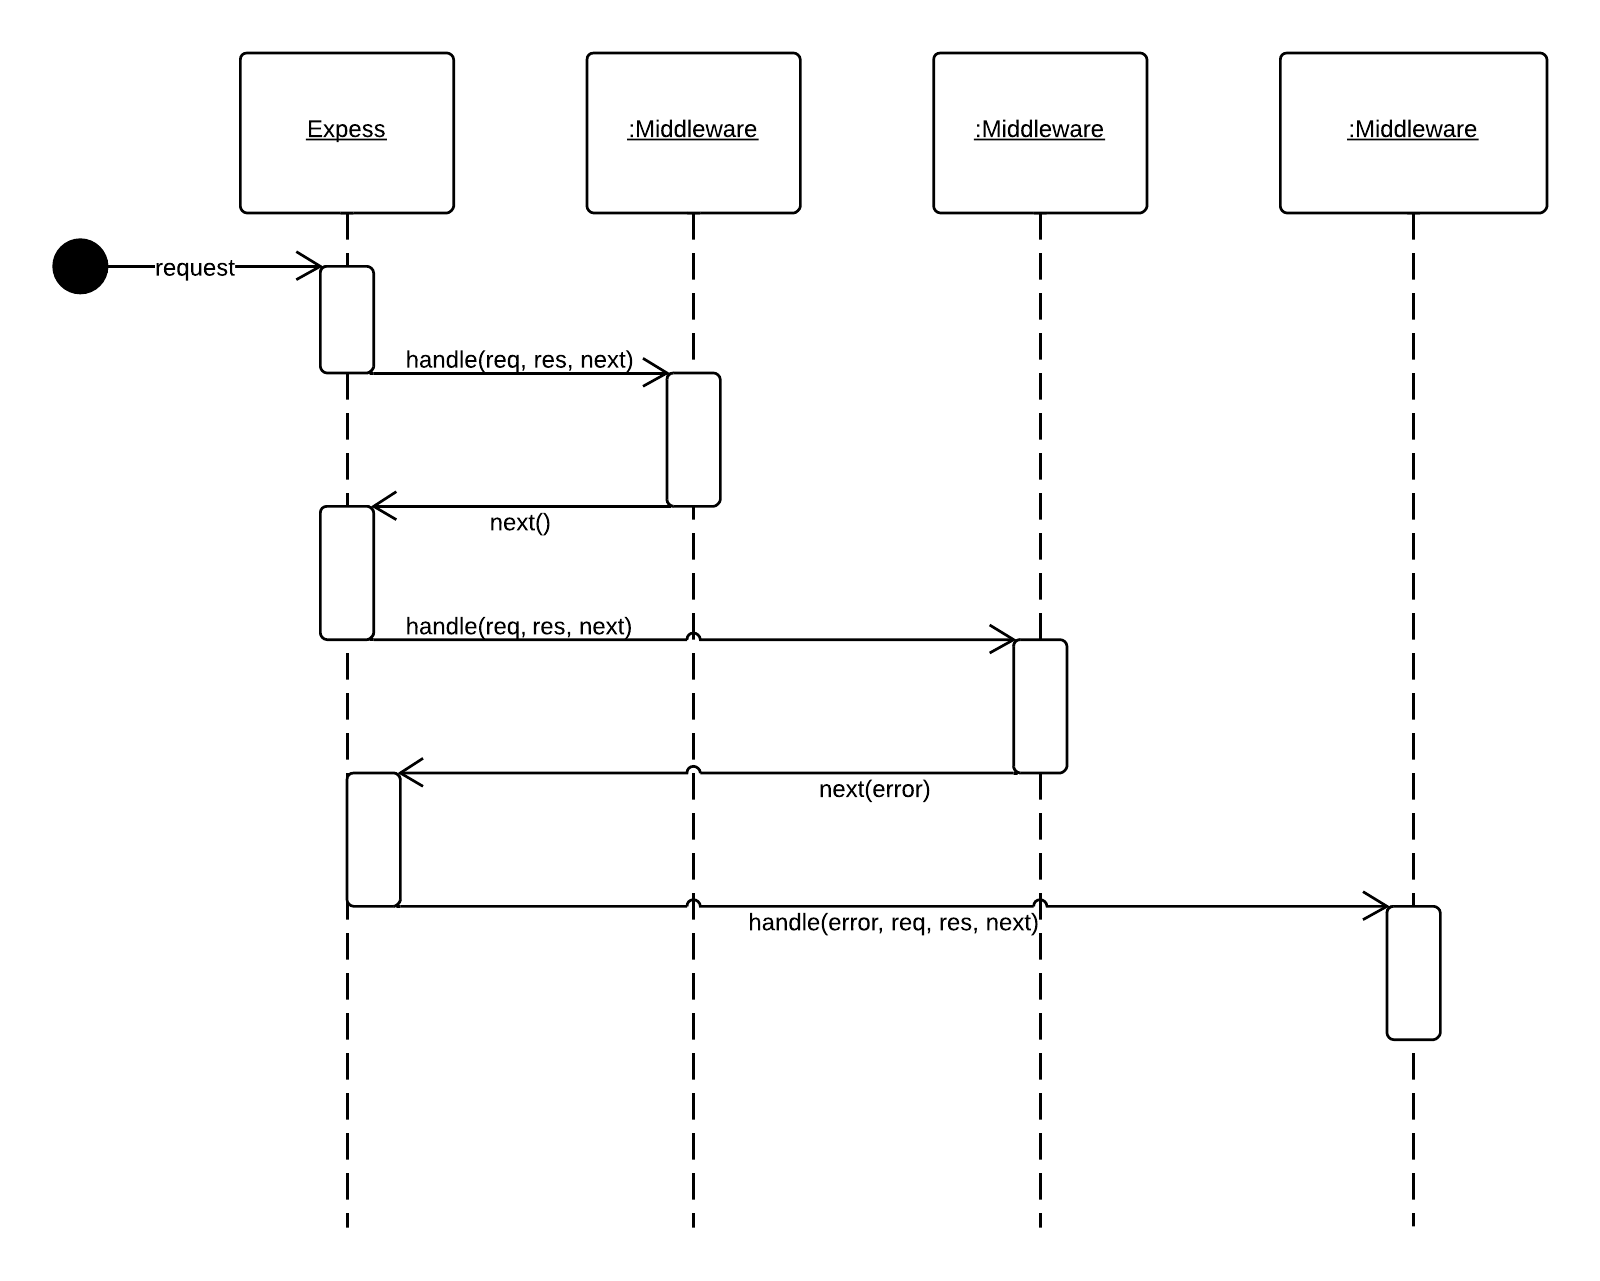
\includegraphics[scale=0.27]{uml/scenari/Diagramma Gestione Richiesta.png}  
		\caption{Diagramma Gestione Richiesta}
	\end{center}  
\end{figure} 

Nel seguente diagramma viene mostrato il comportamento di routing, dove si intende che ogni controllore ha associato un'espressione regolare che specifica su quali richieste agisce. 
\begin{figure}[H]
	\begin{center} 
		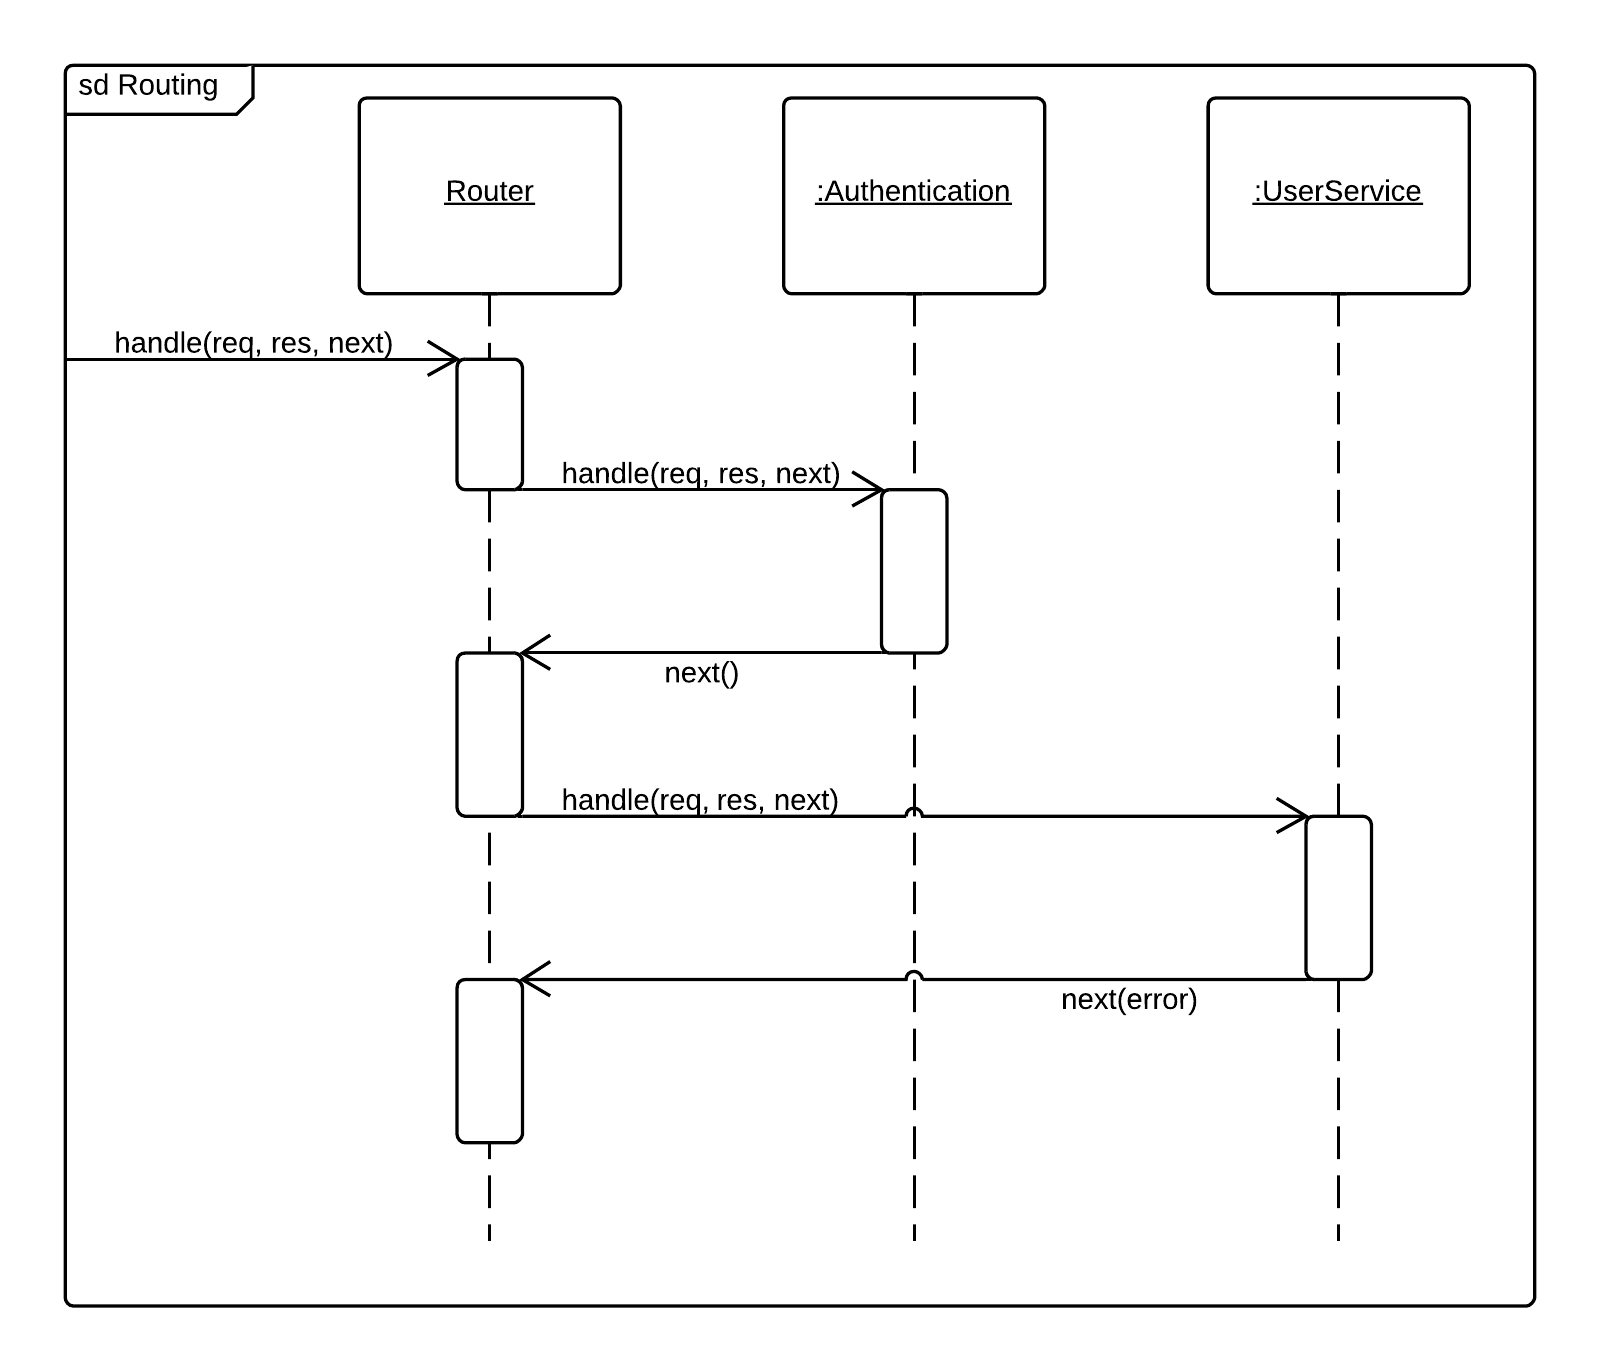
\includegraphics[scale=0.27]{uml/scenari/Diagramma Routing Richiesta.png} 
		\caption{Diagramma Routing Richiesta}
	\end{center} 
\end{figure}

\pagebreak
\subsubsection{Fallimento vincolo ``utente autenticato''}
Per ogni richiesta bisogna verificare che il permesso dell'utente che l'ha chiesta, corrisponda al permesso che la risorsa necessita per poter essere effettuata. \\
Tale scenario rappresenta il fallimento di una richiesta richiedente come vincolo per poter essere effettuata che l'utente abbia un permesso di tipo ''utente autenticato'', dove la verifica dei permessi è gestita dal controller \emph{requireLogged} che manda un next(error) per il fallimento di tale vincolo al router il quale avrà compito di gestirlo.
\begin{figure}[H]
	\begin{center} 
		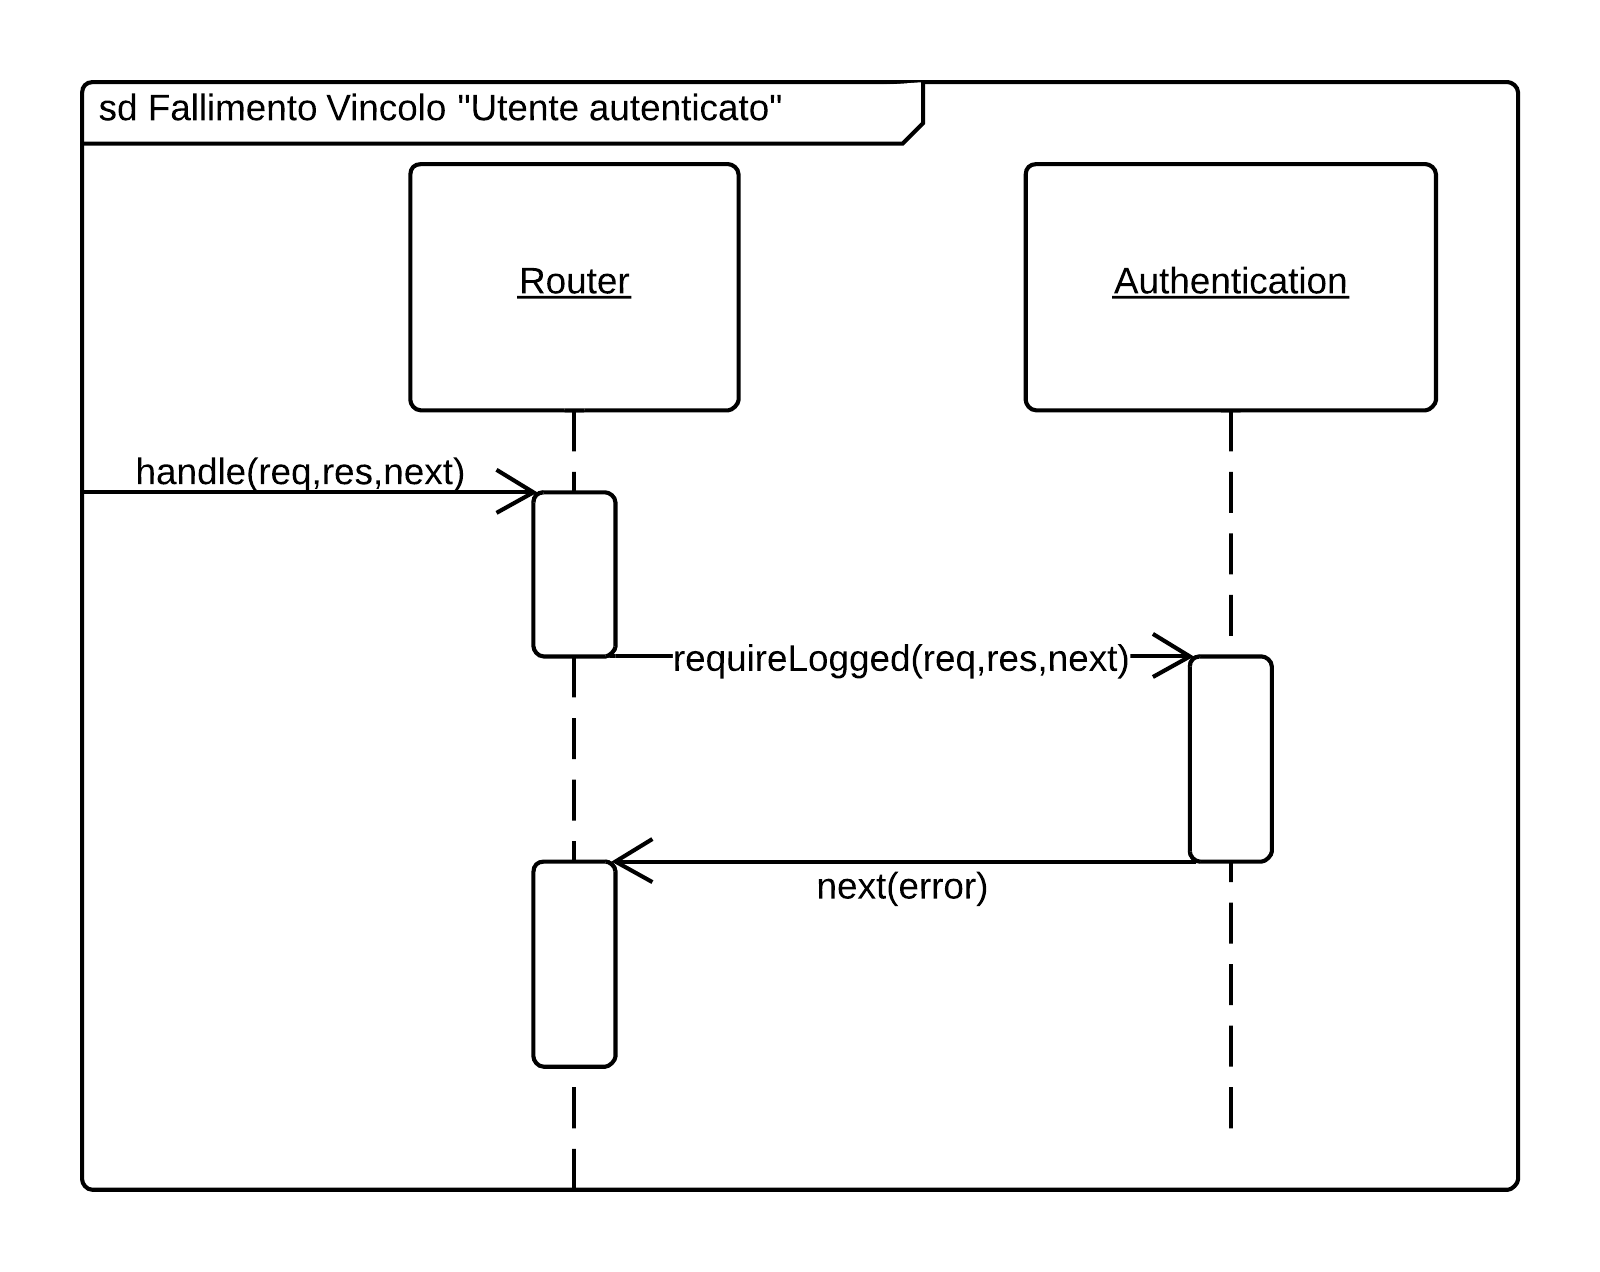
\includegraphics[scale=0.20]{uml/scenari/requireLogged ERROR.png} 
		\caption{Fallimento vincolo ``utente autenticato''}
	\end{center} 
\end{figure}

\pagebreak
\subsubsection{Fallimento vincolo ``utente non autenticato''}
Il seguente diagramma di sequenza rappresenta lo scenario in cui fallisce la verifica del vincolo di permesso ''utente autenticato''.
La richiesta viene gestita da \emph{requireNotLogged} che verifica con esito negativo i permessi e rimanda un next(error) al router.
\begin{figure}[H]
	\begin{center} 
		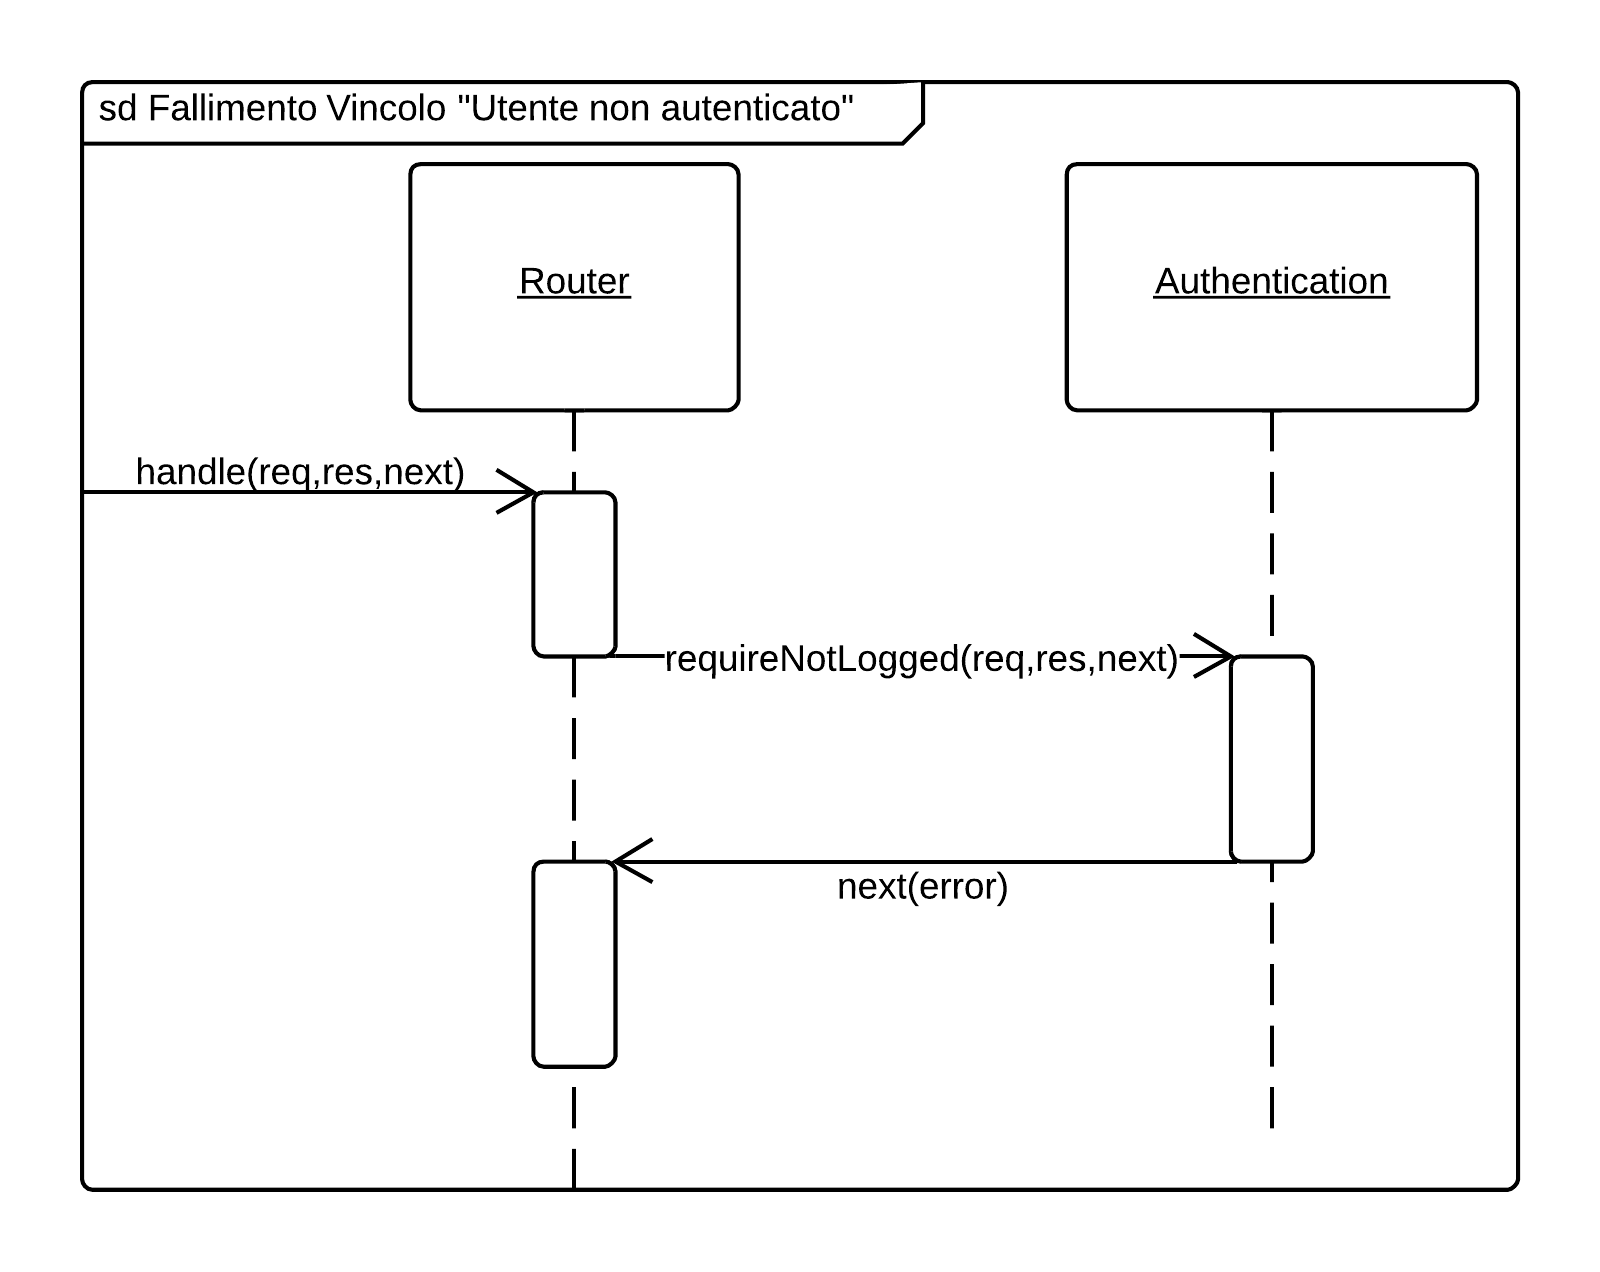
\includegraphics[scale=0.20]{uml/scenari/requireNotLogged ERROR.png} 
		\caption{Fallimento vincolo ``utente non autenticato''}
	\end{center} 
\end{figure}

\pagebreak
\subsubsection{Fallimento vincolo ``utente admin''}
Nel diagramma seguente viene rappresentato lo scenario in cui si richiedono permessi ''Admin'' per poter gestire la richiesta corrispondente e la verifica effettuata dal controller \emph{requireAdmin} fallisce. 
\begin{figure}[H]
	\begin{center} 
		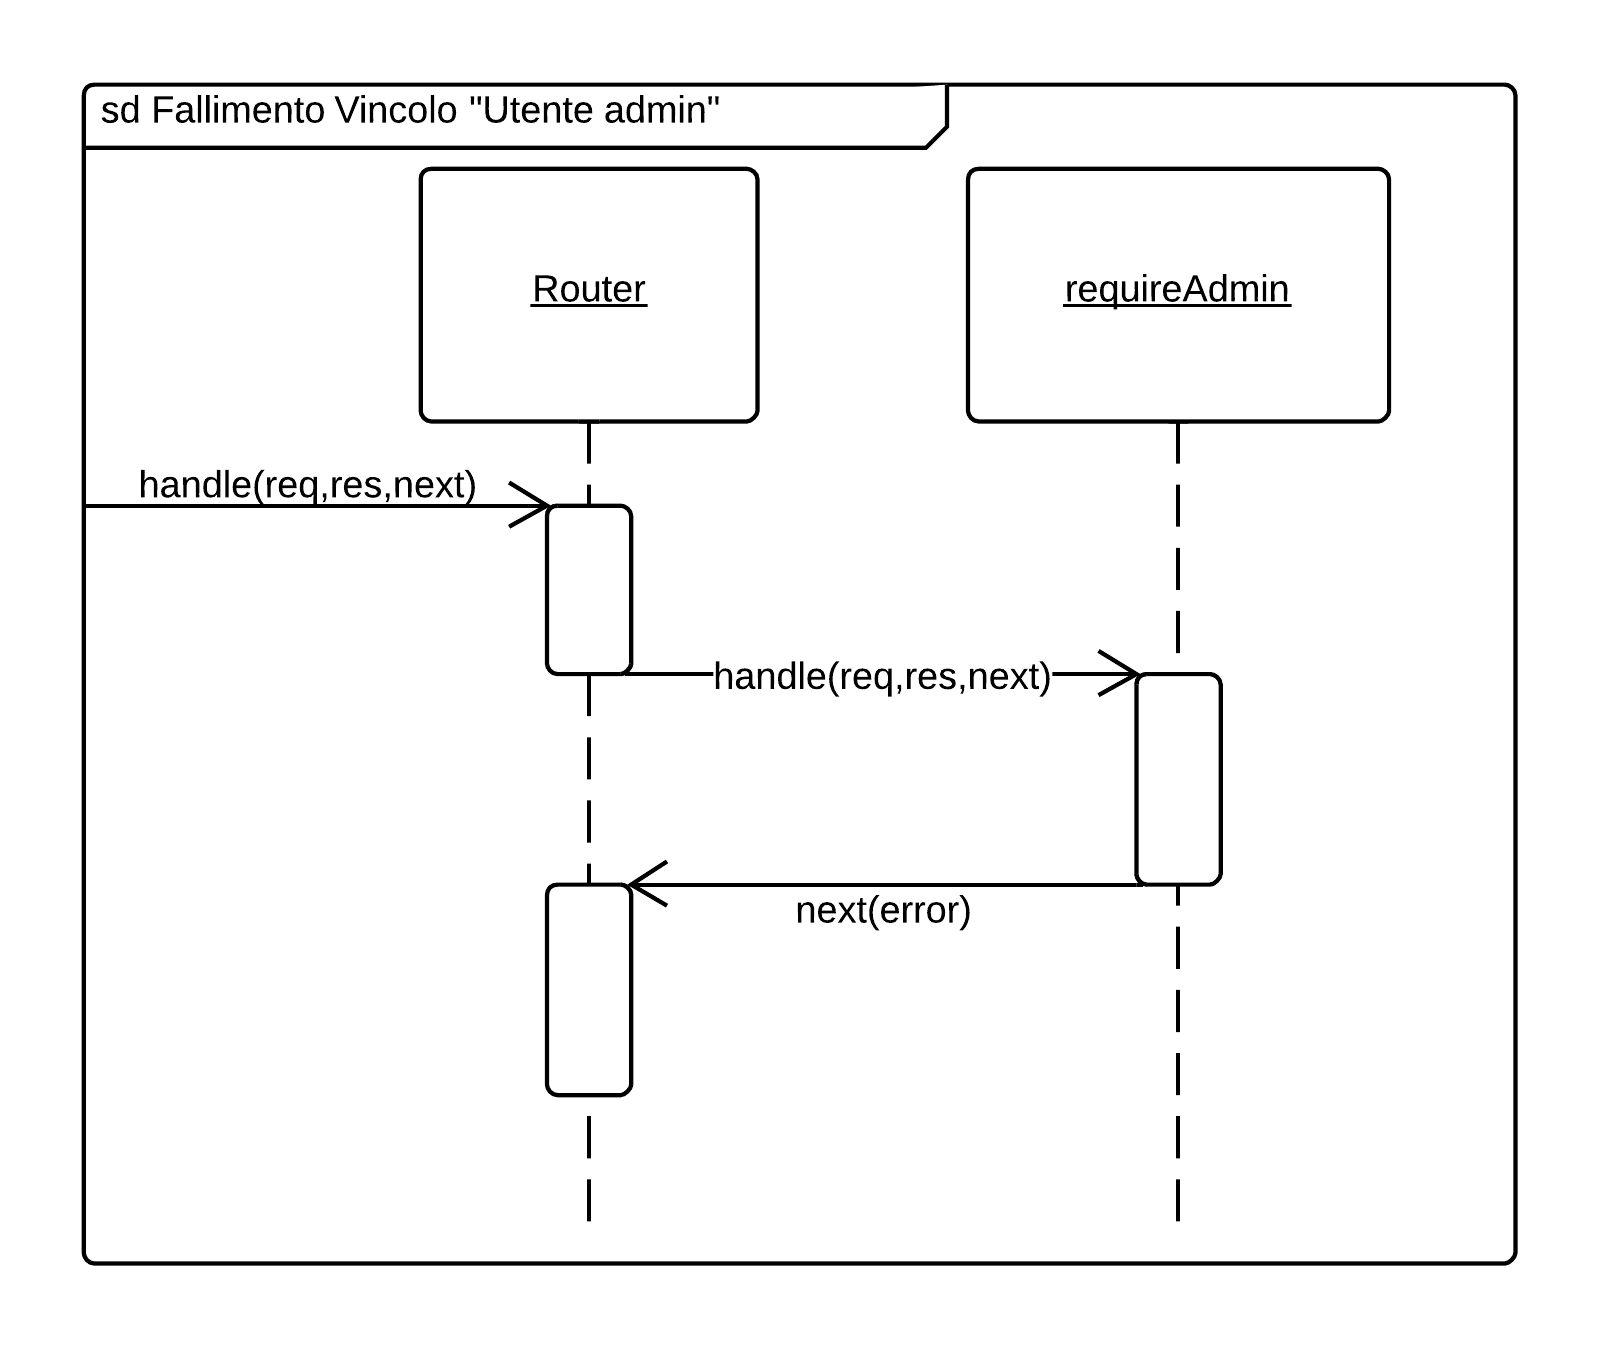
\includegraphics[scale=0.20]{uml/scenari/requireAdmin ERROR.png} 
		\caption{Fallimento vincolo ``utente admin''}
	\end{center} 
\end{figure}

\pagebreak
\subsubsection{Fallimento vincolo ``utente  super admin''}
Nel diagramma seguente viene rappresentato lo scenario in cui si richiedono permessi ''Super Admin'' per poter gestire la richiesta corrispondente e la verifica effettuata dal controller \emph{requireSuperAdmin} fallisce. 
\begin{figure}[H]
	\begin{center} 
		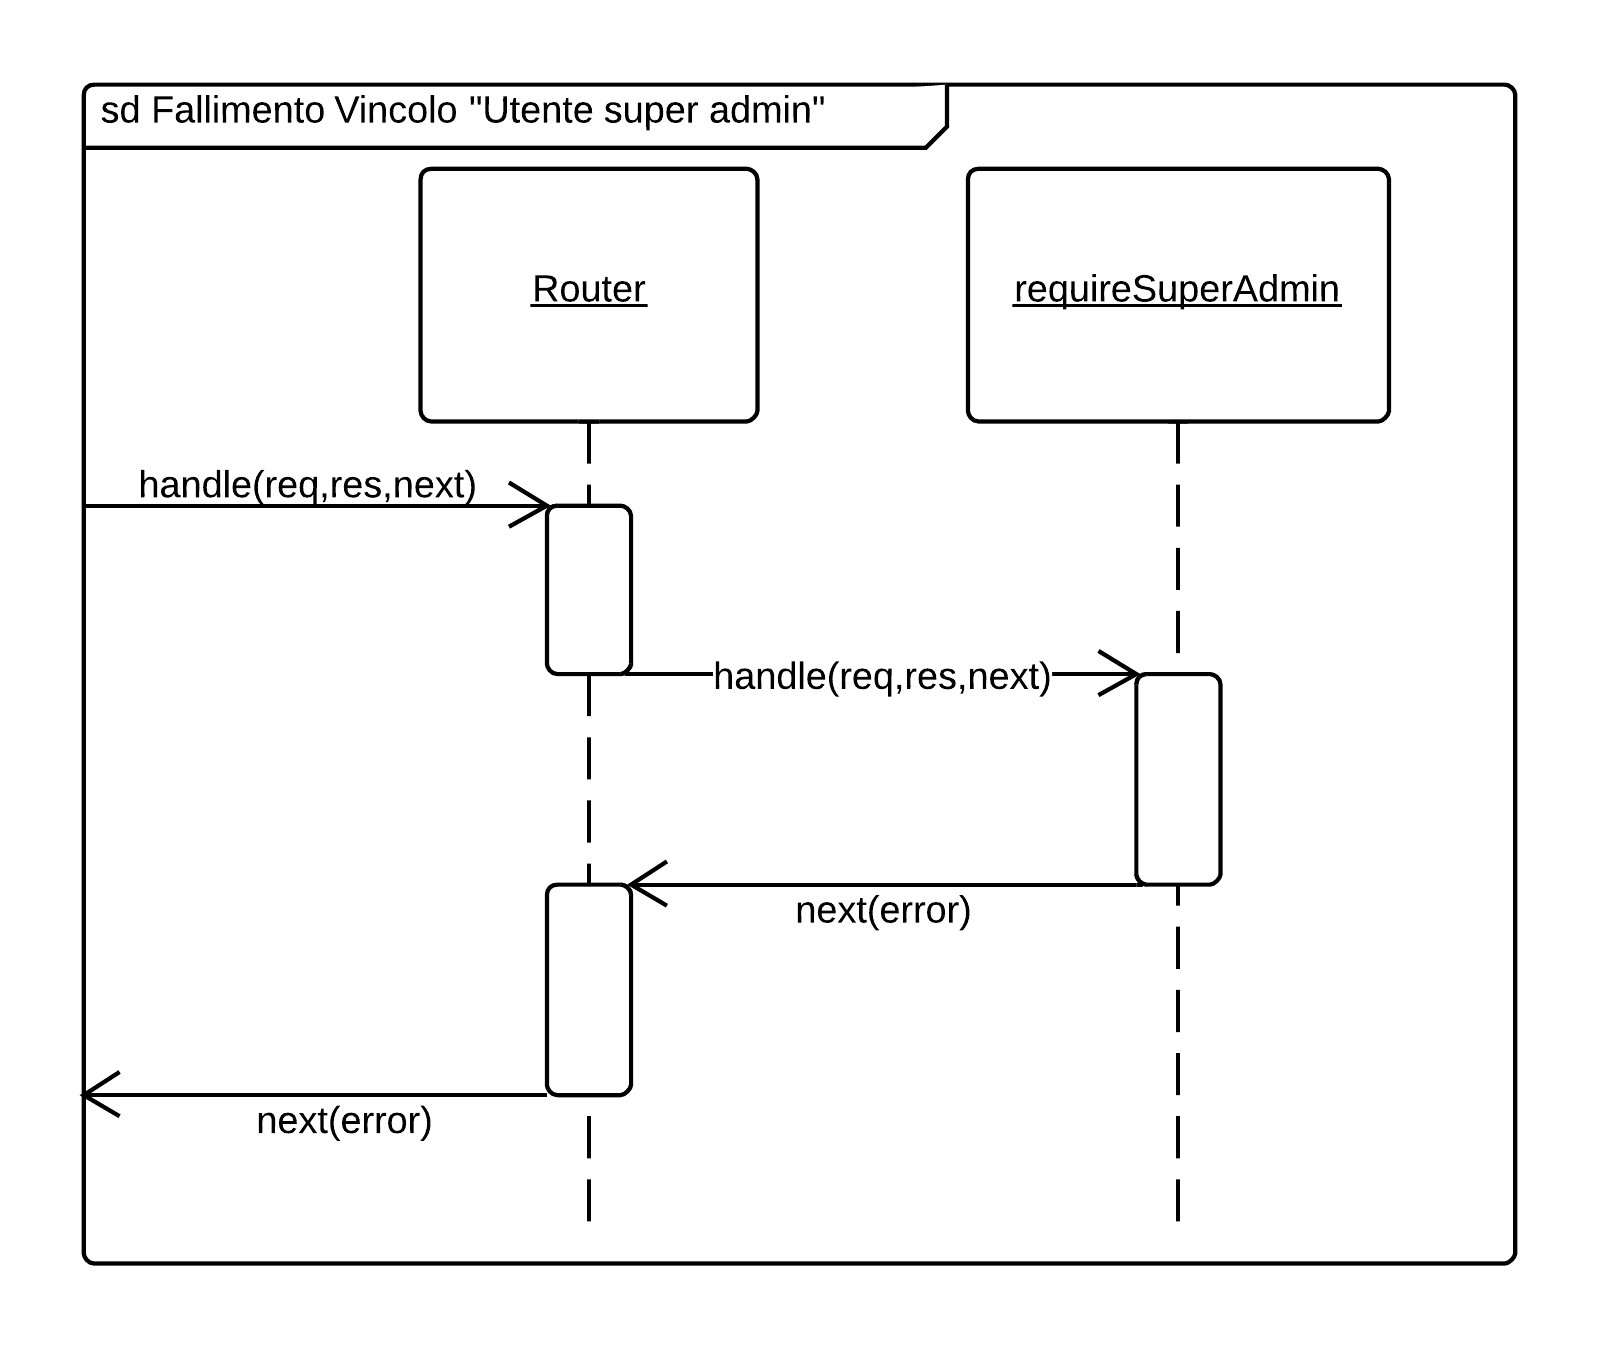
\includegraphics[scale=0.20]{uml/scenari/requireSuperAdmin ERROR.png} 
		\caption{Fallimento vincolo ``utente super admin''}
	\end{center} 
\end{figure}

\pagebreak
\subsubsection{Richiesta POST /login} 
Il seguente scenario mostra la gestione di una richiesta POST per la risorsa di login, \emph{requireNotLogged} non risponde con errore, chiamando il successivo \glossario{middleware} \emph{login} che gestisce la verifica dei parametri e nell'opzione che questa fallisca, manda in risposta un next(error) che il router andrà a gestire.
\begin{figure}[H]
	\begin{center} 
		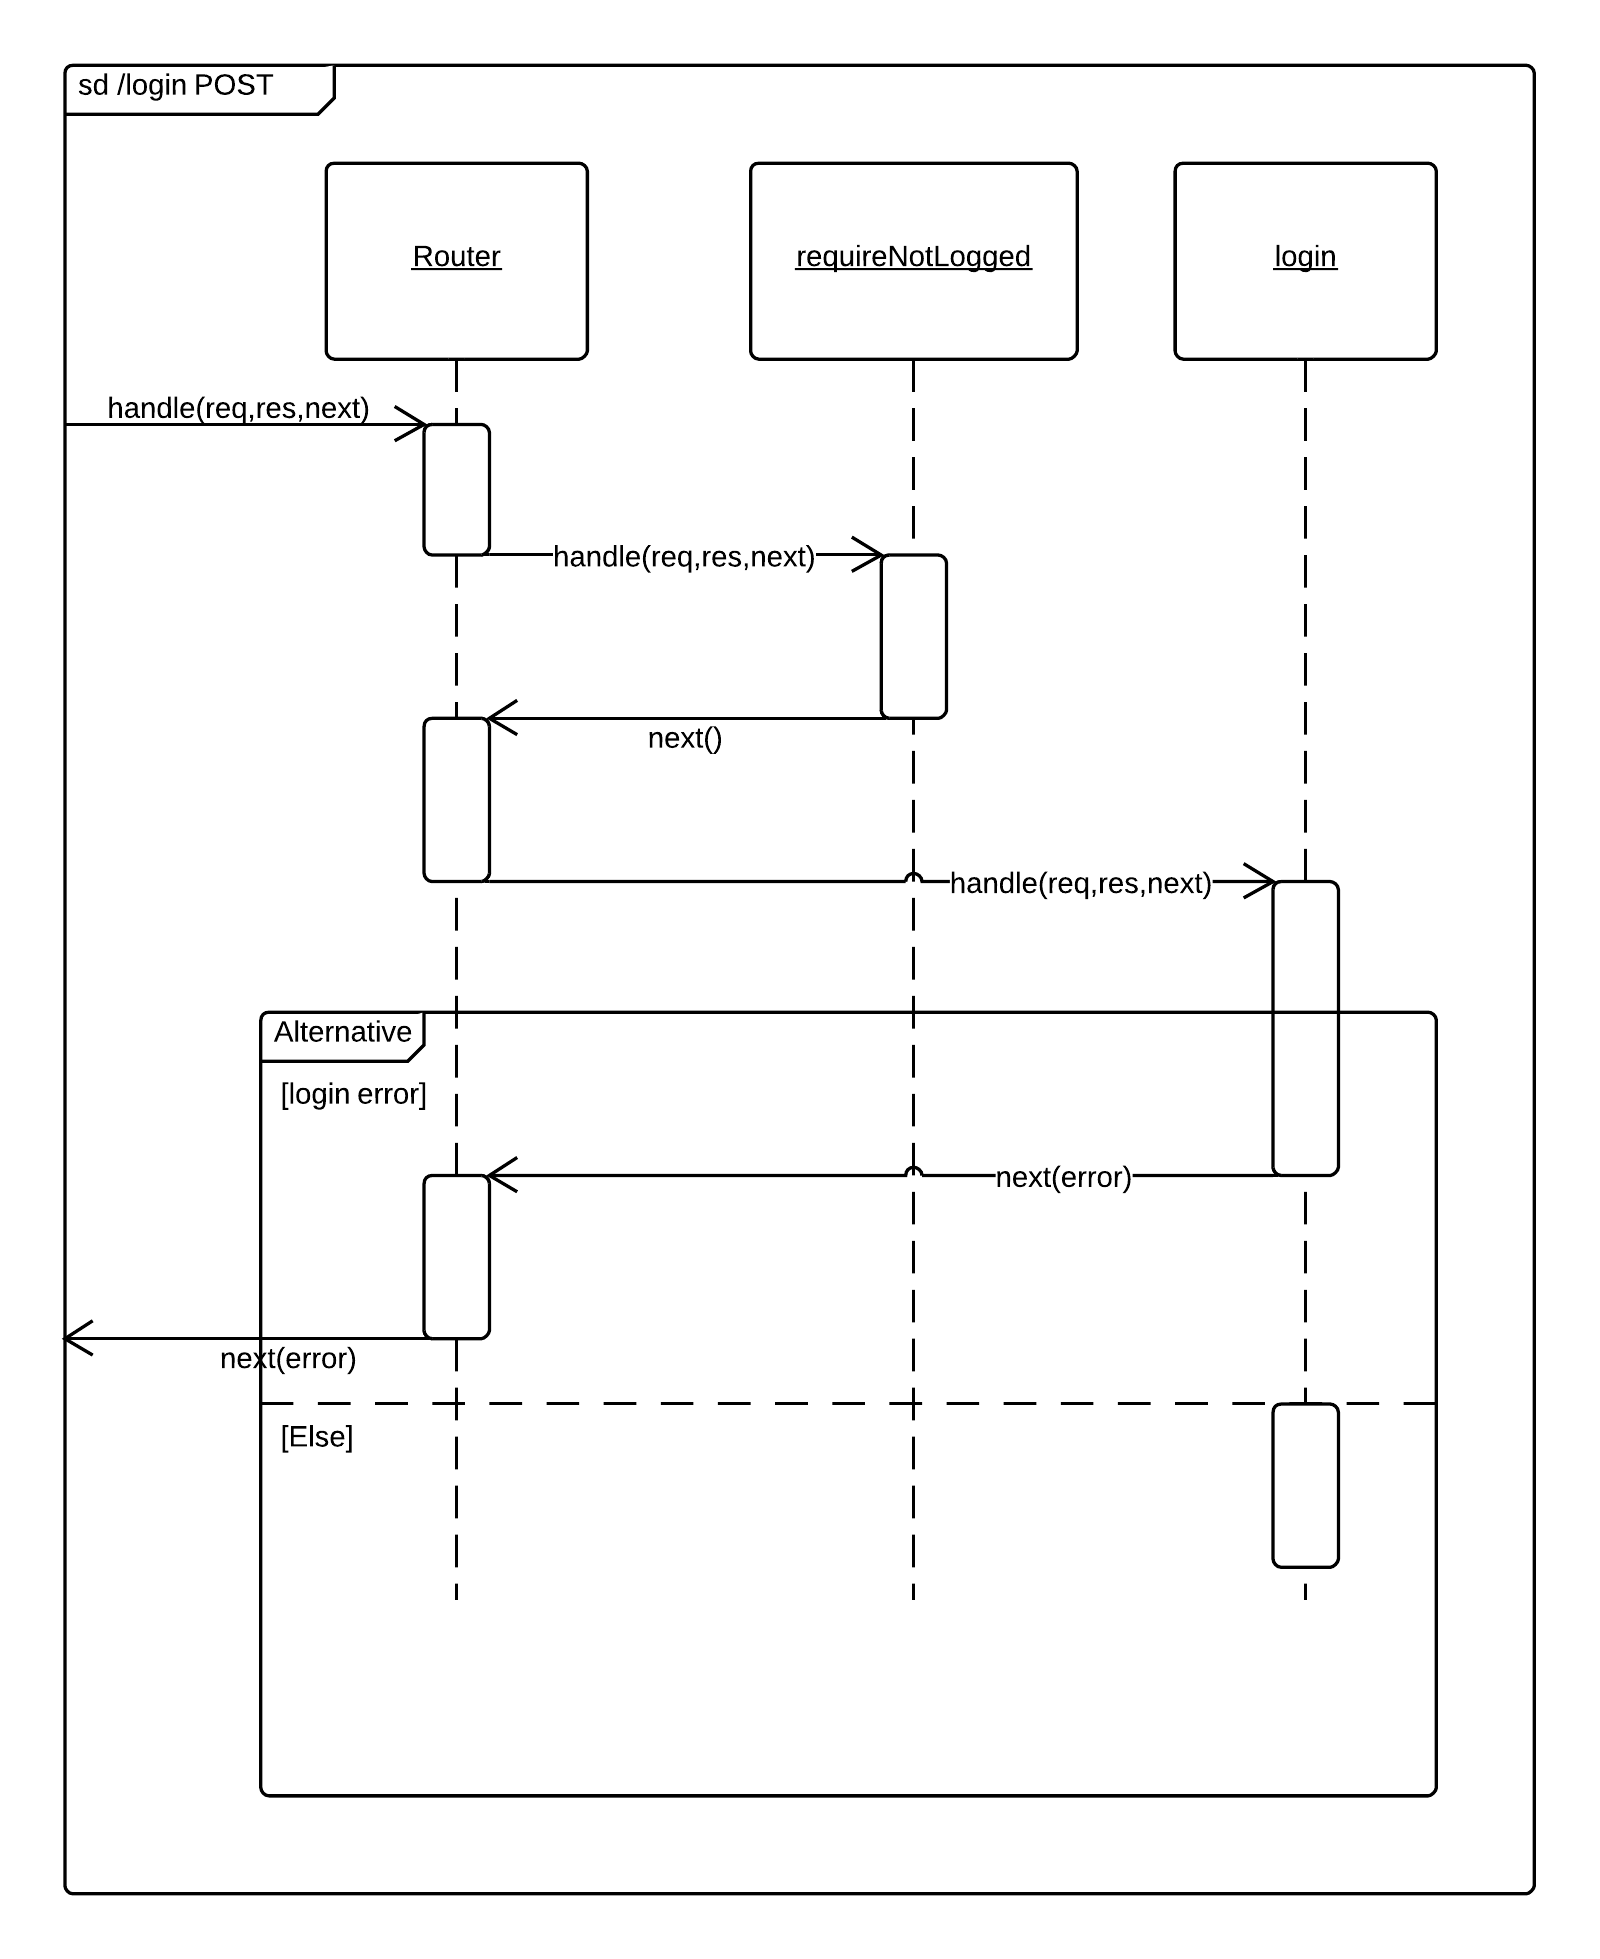
\includegraphics[scale=0.20]{uml/scenari/login POST.png} 
		\caption{Richiesta POST /login}
	\end{center} 
\end{figure} 

\pagebreak
\subsubsection{Richiesta DELETE /logout}
Il diagramma di sequenza mostra lo scenario di una richiesta DELETE per la risorsa login.
La verifica dei permessi in \emph{requireLogged} non fallisce, innescando la chiamata al successivo \glossario{middleware} \emph{logout} che gestisce l'eliminazione della risorsa.
\begin{figure}[H]
	\begin{center} 
		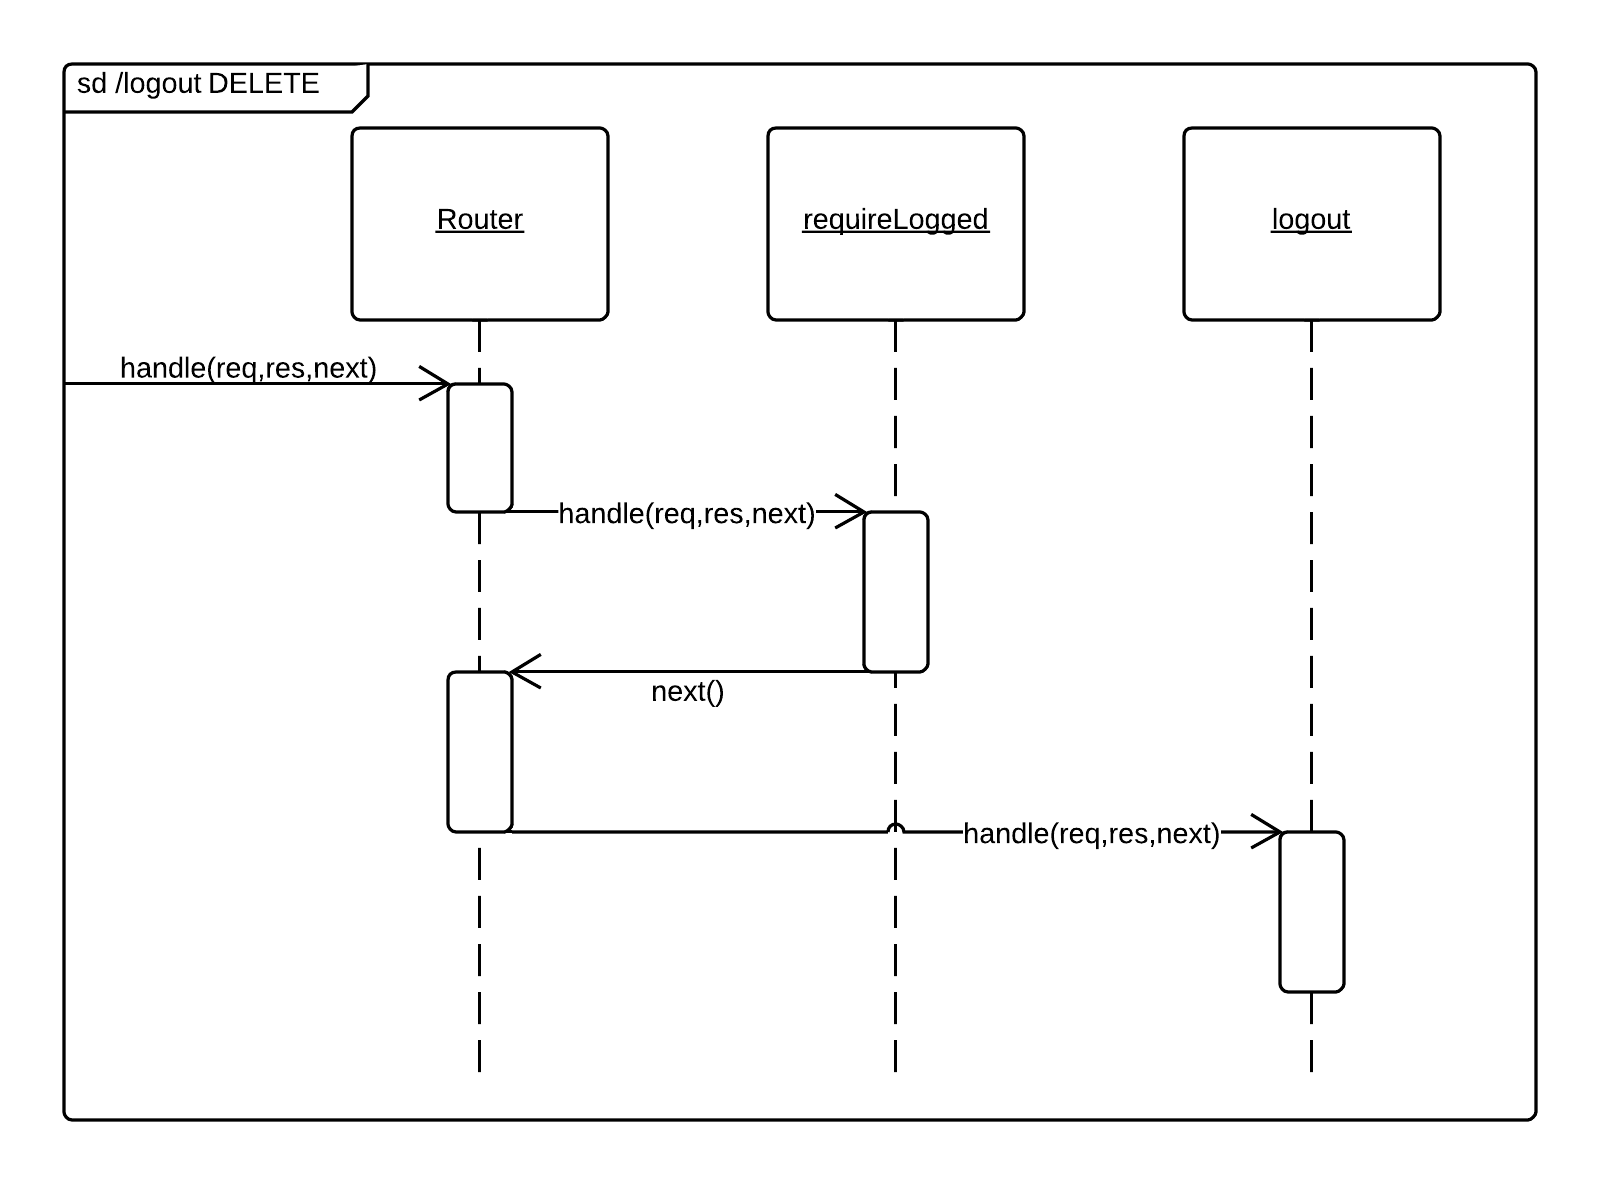
\includegraphics[scale=0.20]{uml/scenari/logout DELETE.png} 
		\caption{Richiesta DELETE /logout}
	\end{center} 
\end{figure}

\pagebreak
\subsubsection{Richiesta GET /profile}
Il seguente diagramma rappresenta lo scenario di una richiesta GET per ottenere la risorsa Profile, la verifica dei permessi non fallisce e la richiesta viene gestita da \emph{getProfile}.
\begin{figure}[H]
	\begin{center} 
		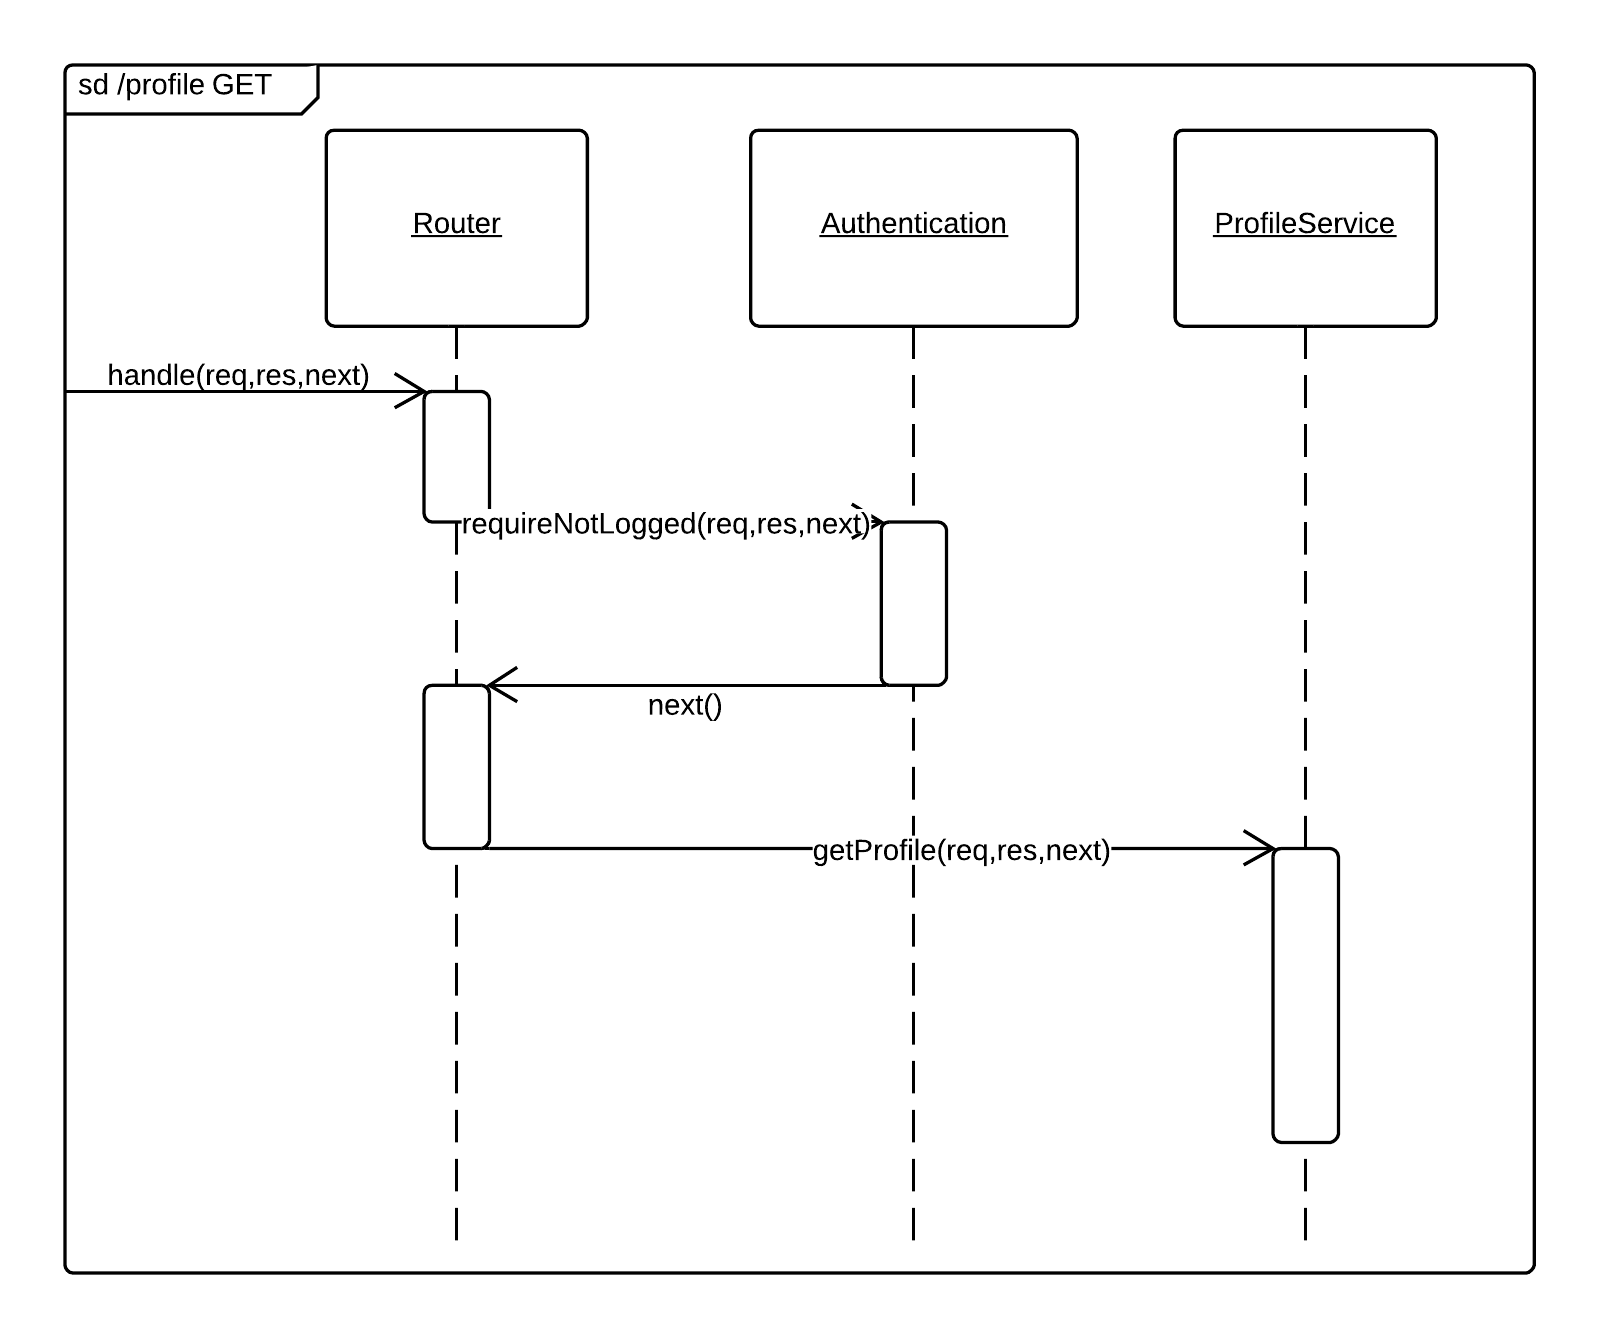
\includegraphics[scale=0.20]{uml/scenari/Profile GET.png} 
		\caption{Richiesta GET /profile}
	\end{center} 
\end{figure}

\pagebreak
\subsubsection{Richiesta PUT /profile} 
Viene rappresentato lo scenario di una richiesta PUT per la risorsa Profile, il \emph{requireLogged} non ritorna un errore, chiamando il successivo \glossario{middleware} \emph{editProfile} che gestisce la richiesta di modifica dei dati del profilo.
Nell'opzione che i parametri passati per la modifica del profilo siano errati, \emph{editProfile} chiamerà la callback passandogli la descrizione dell'errore come parametro che il router andrà a gestire.
\begin{figure}[H]
	\begin{center} 
		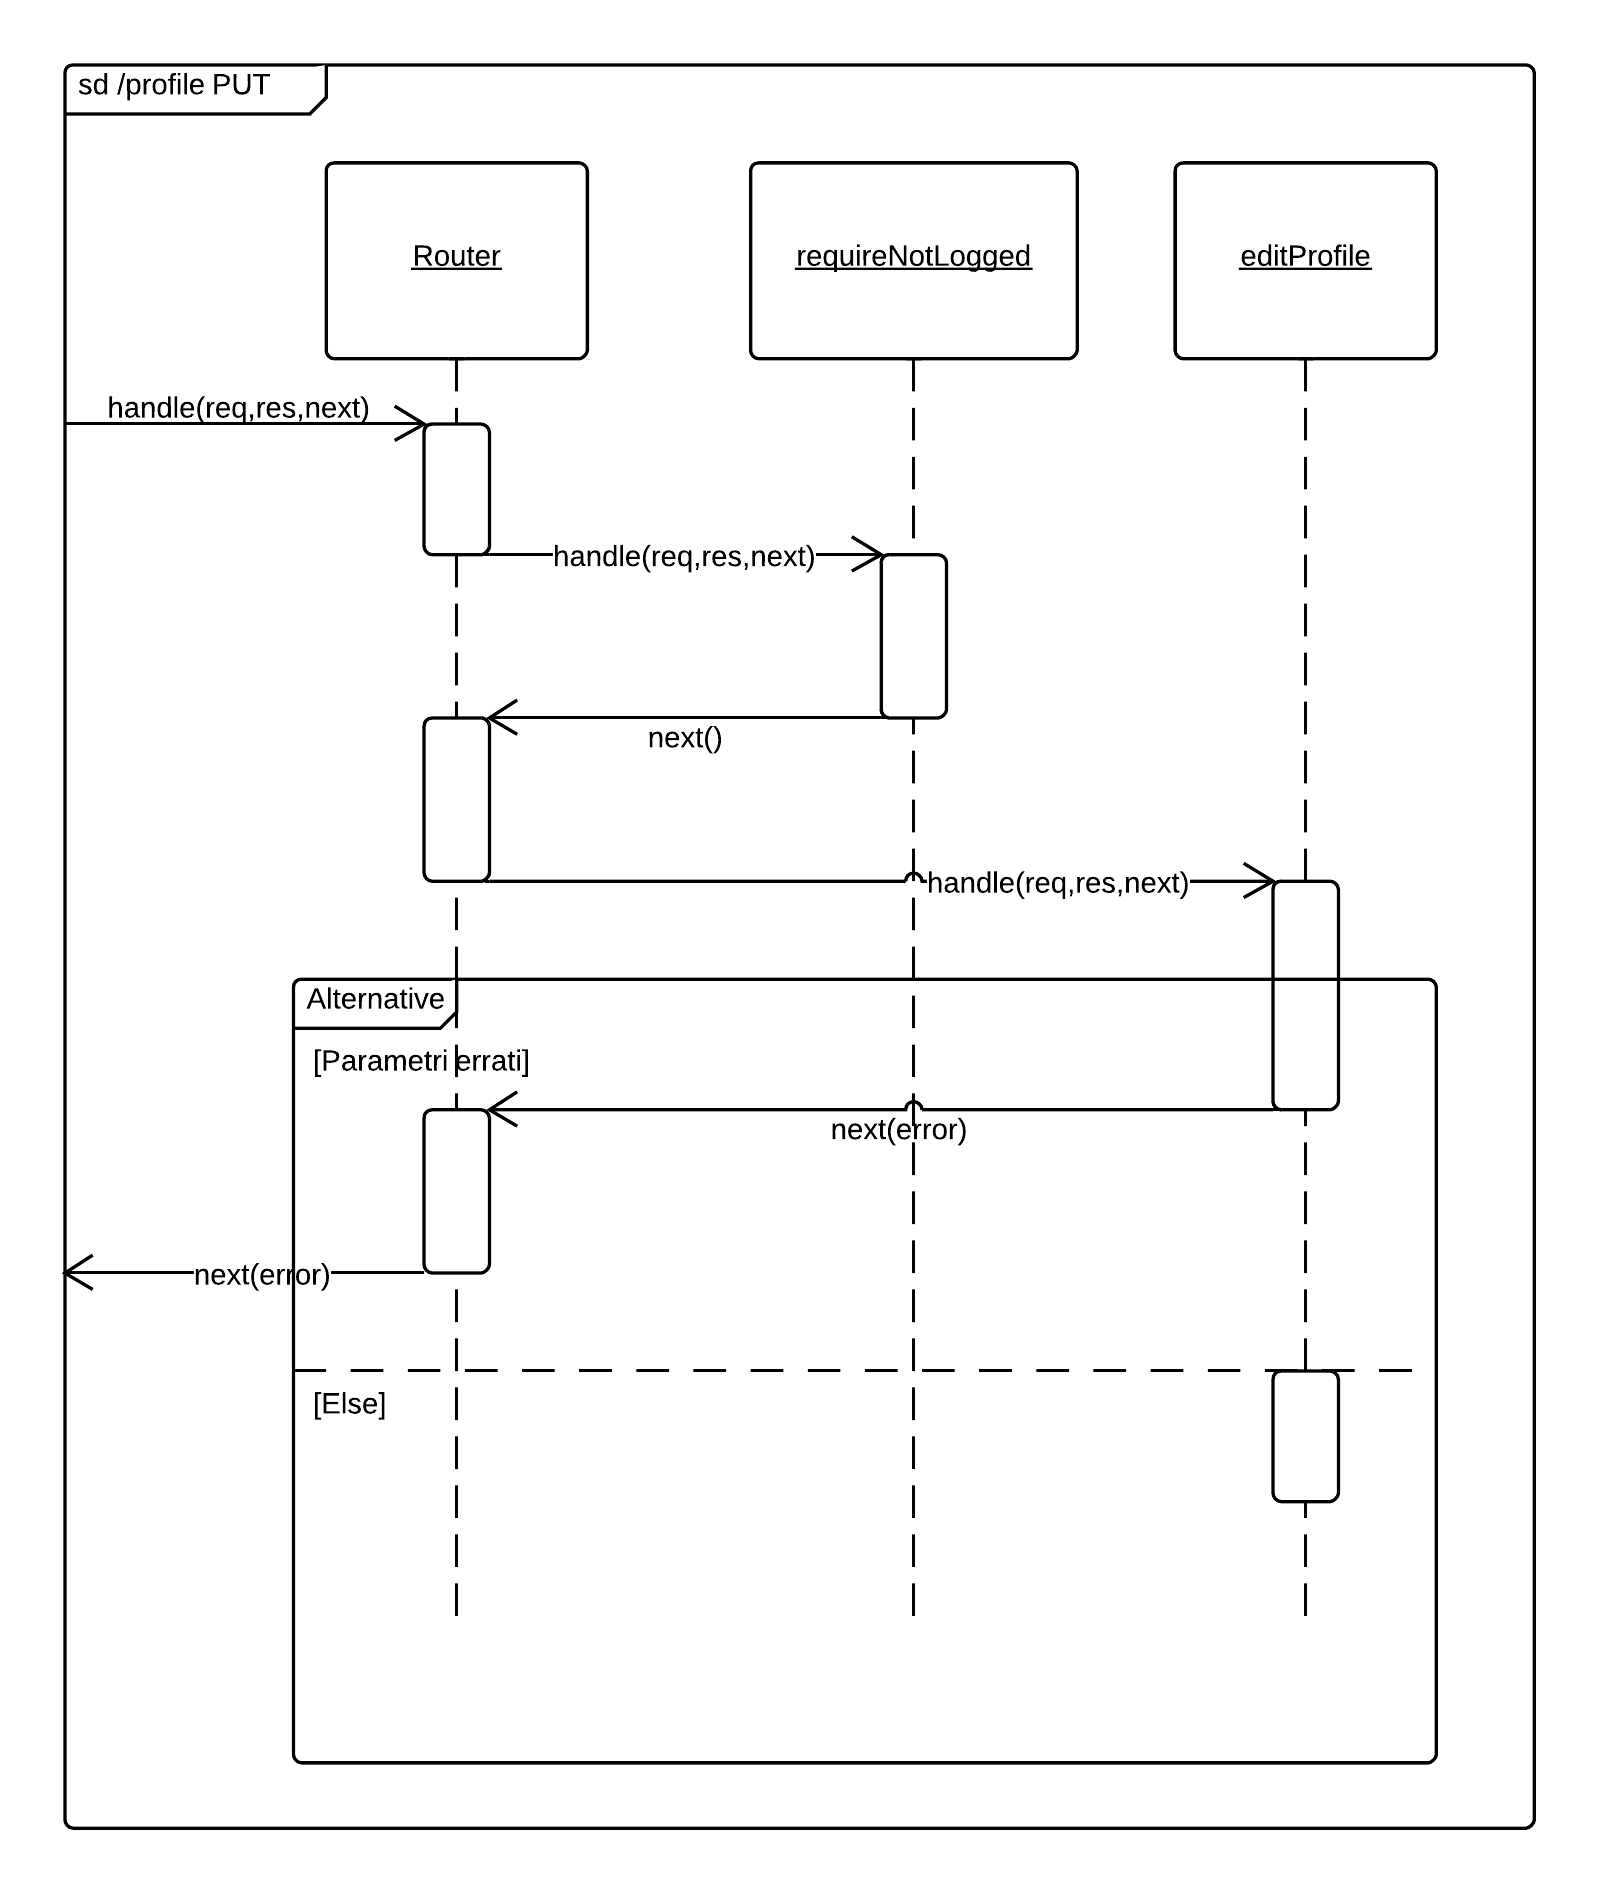
\includegraphics[scale=0.20]{uml/scenari/Profile PUT.png} 
		\caption{Richiesta PUT /profile}
	\end{center} 
\end{figure}

\pagebreak
\subsubsection{Richiesta POST /password/forgot} 
Viene rappresentato lo scenario di una richiesta POST per la risorsa password forgot, il \emph{requireNotLogged} non risponde errore e il controllo passa a \emph{passwordResetRequest} che gestisce la richiesta.
Se i parametri passati per la richiesta sono errati, il controllore \emph{requireNotLogged} risponderà con un errore.
\begin{figure}[H]
	\begin{center} 
		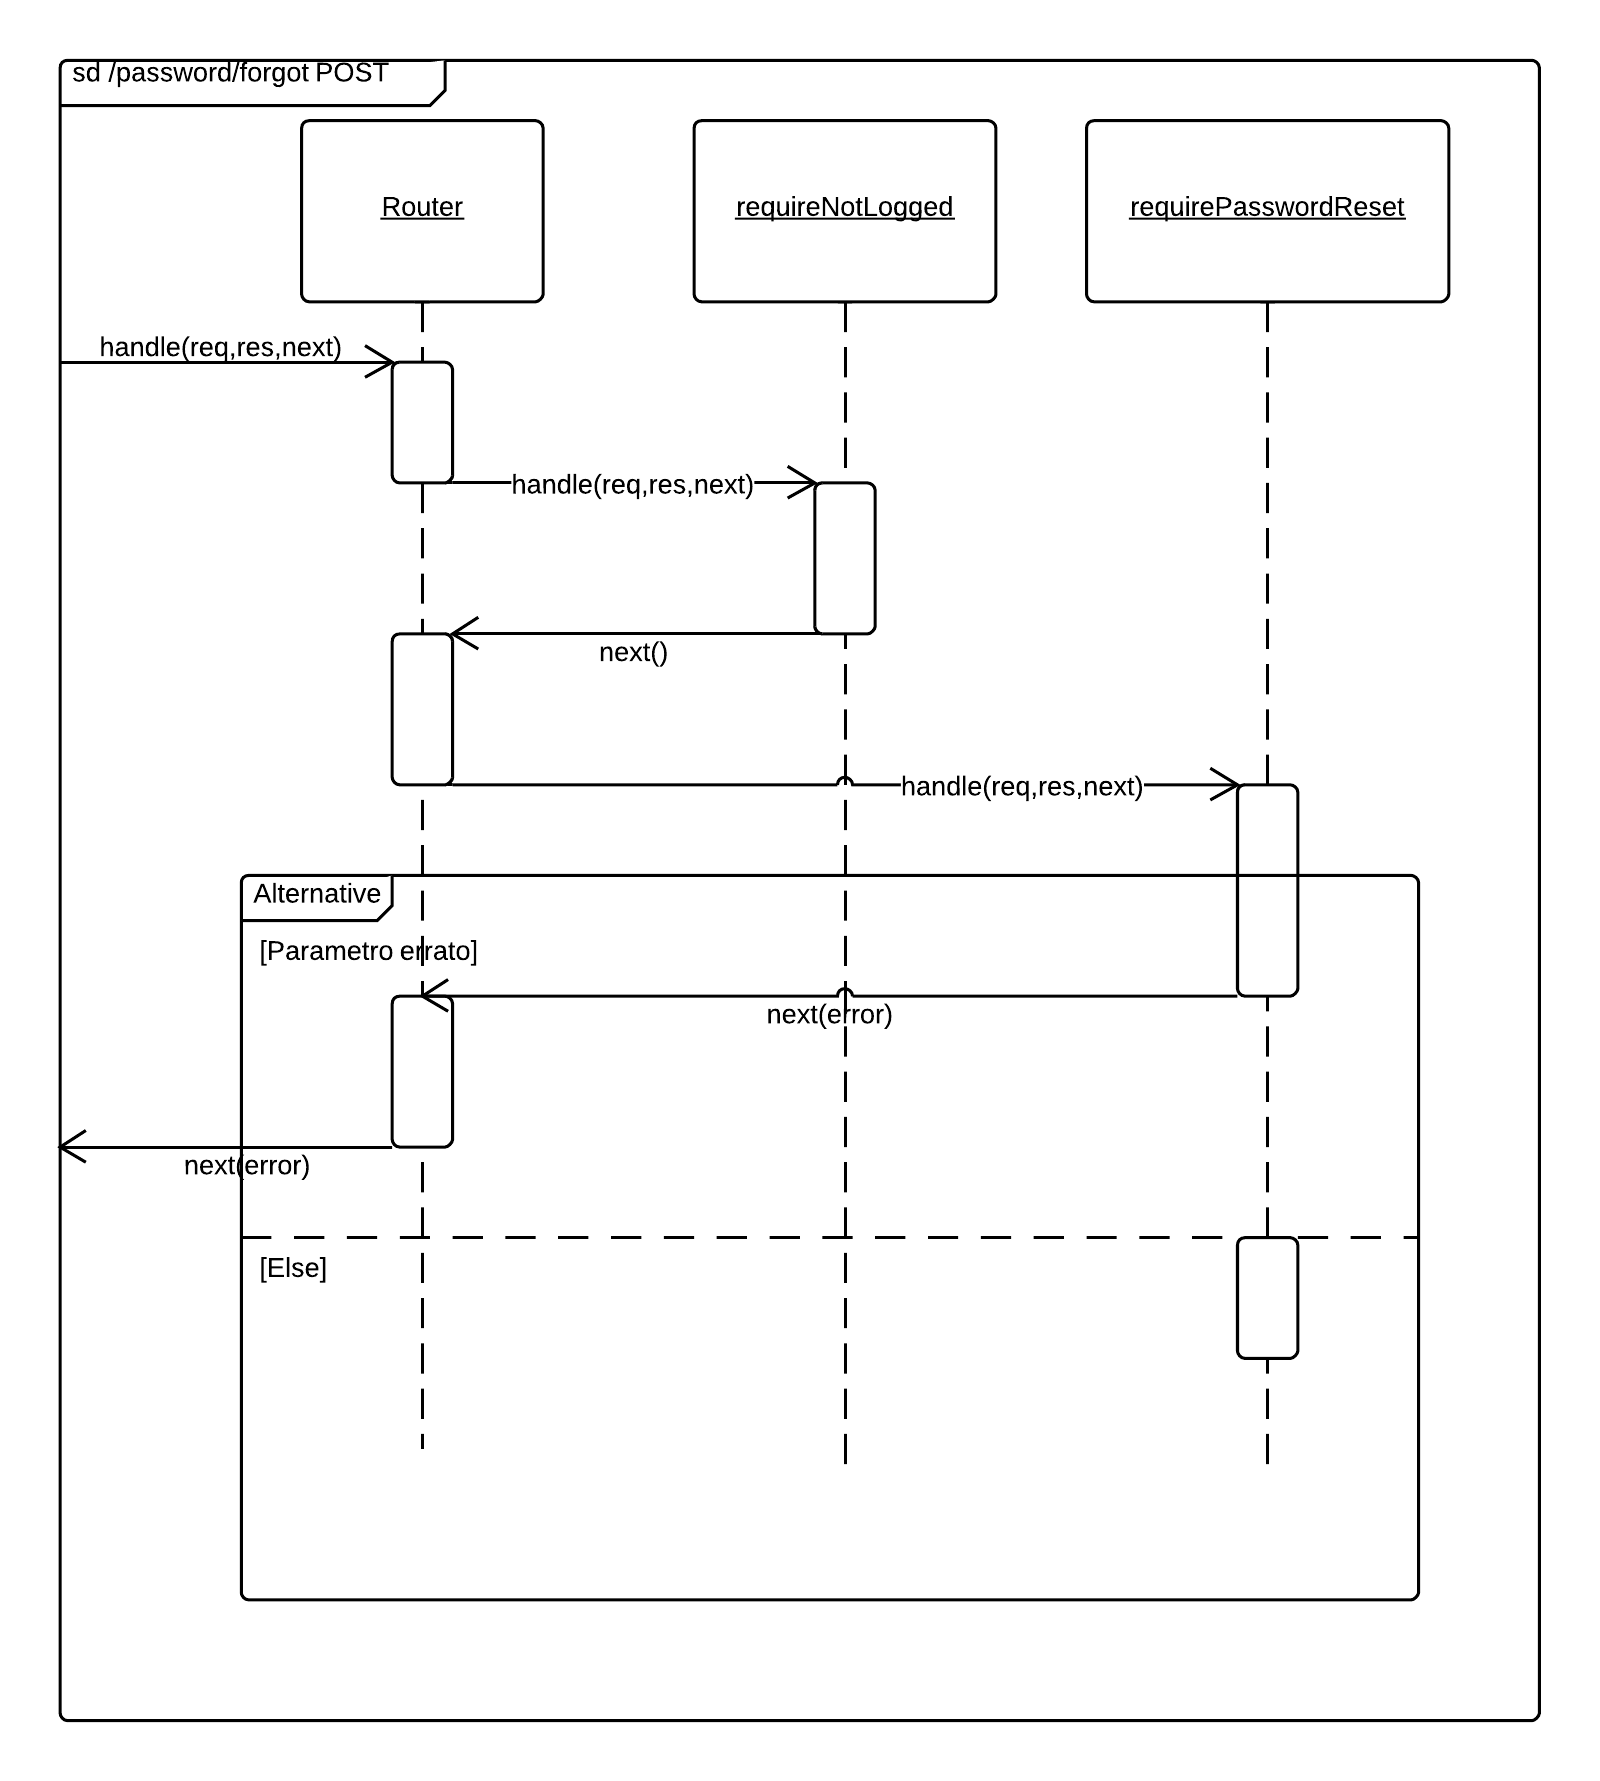
\includegraphics[scale=0.20]{uml/scenari/Password Forgot POST.png} 
		\caption{Richiesta POST /password/forgot}
	\end{center} 
\end{figure}

\pagebreak
\subsubsection{Richiesta GET /users}
Viene rappresentato nel seguente diagramma di sequenza lo scenario di una richiesta GET per la risorsa user, \emph{requireAdmin} non fallisce ed il controllo viene passato a \emph{getUsers} che gestisce la richiesta.
\begin{figure}[H]
	\begin{center} 
		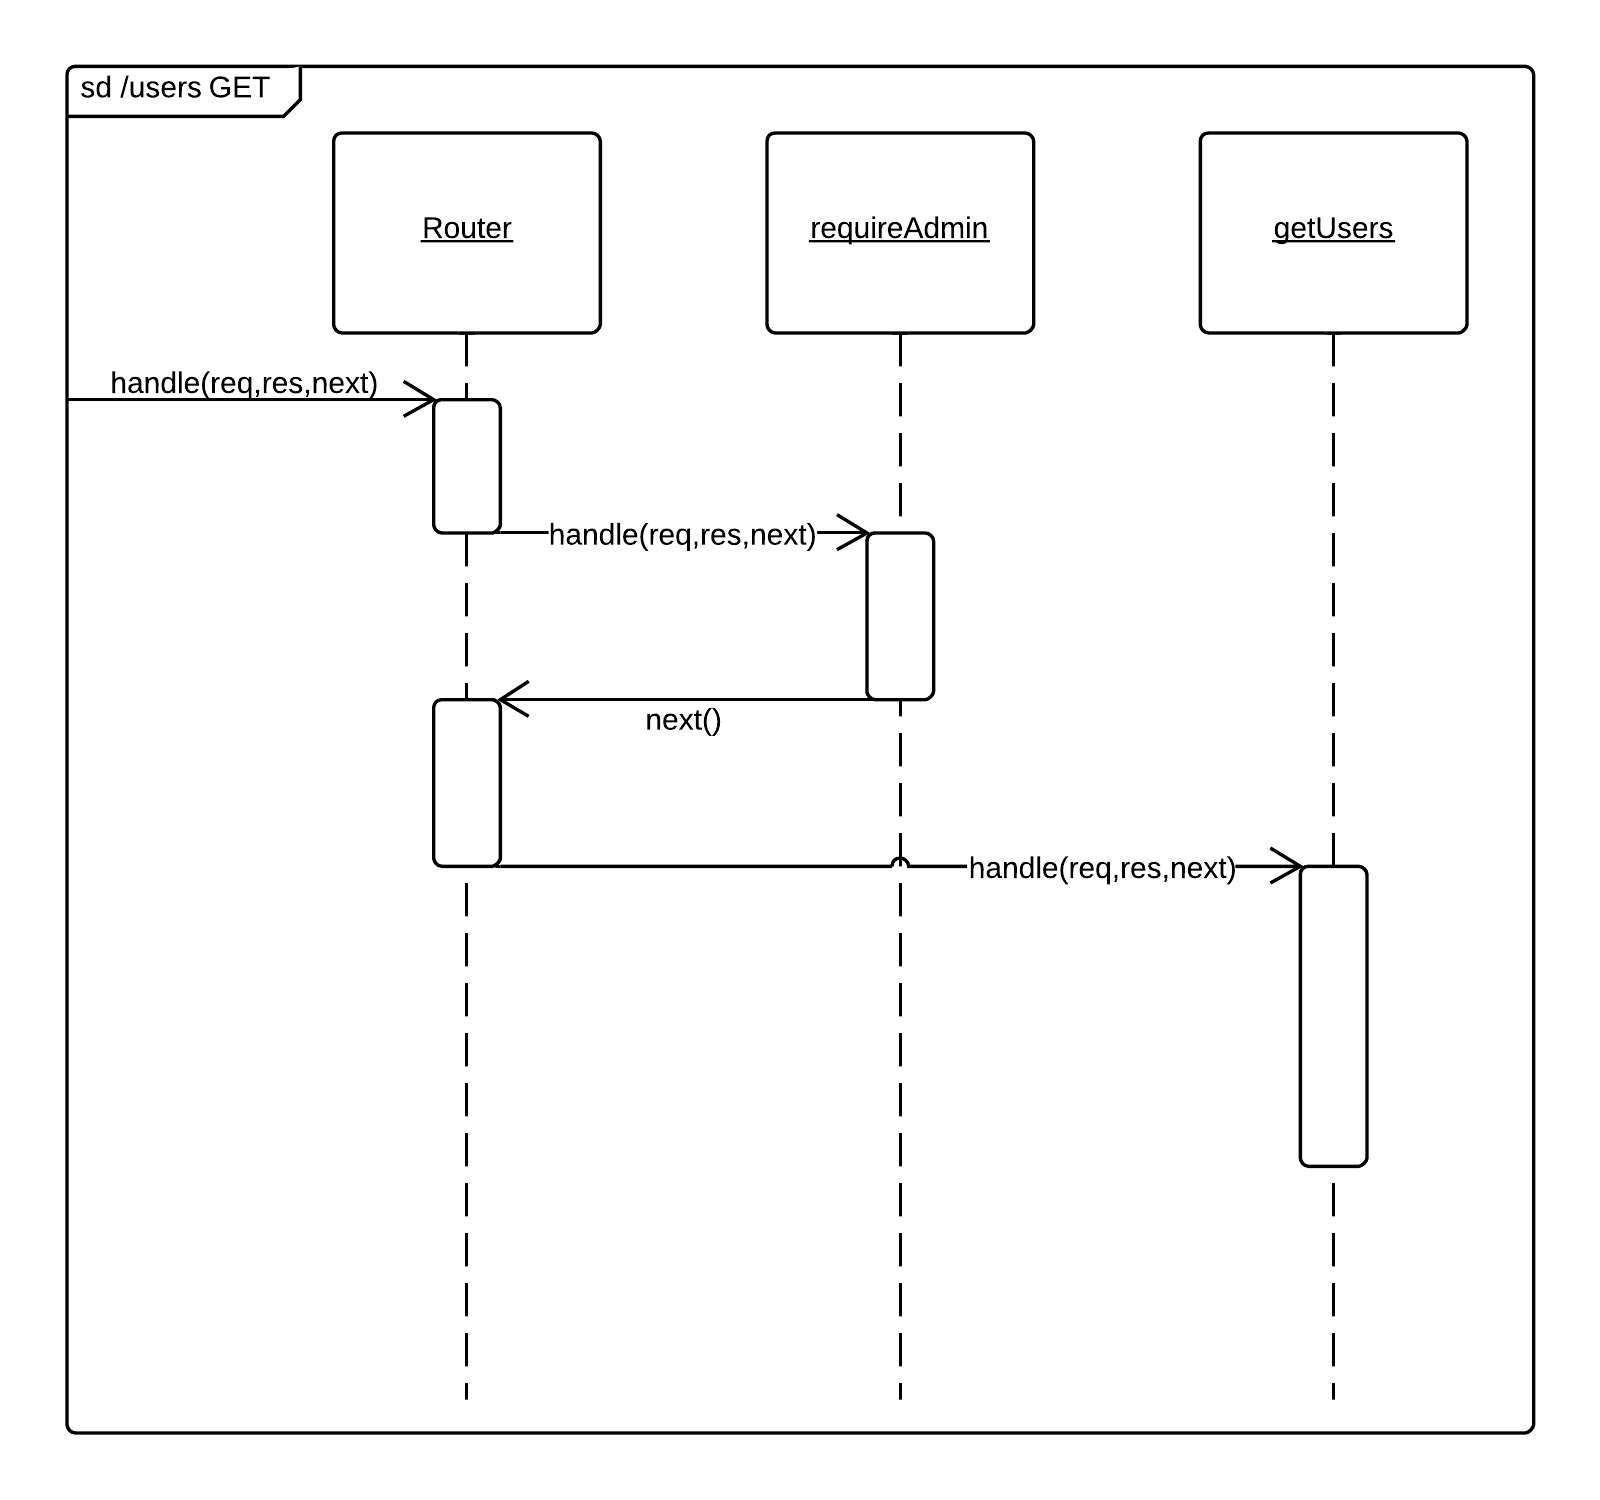
\includegraphics[scale=0.20]{uml/scenari/Users GET.png} 
		\caption{Richiesta GET /users}
	\end{center} 
\end{figure}

\pagebreak
\subsubsection{Richiesta POST /users} 
Il seguente diagramma di sequenza rappresenta lo scenario di una richiesta POST per la risorsa user, la verifica di \emph{requireLogged} dei permessi utente non fallisce e viene passato il controllo a \emph{createUser} che gestisce la richiesta di creazione di un nuovo user, e nel caso la verifica dei parametri passati per la creazione di quest'ultimo siano errati, il controllore chiamerà la callback con l'errore.
\begin{figure}[H]
	\begin{center} 
		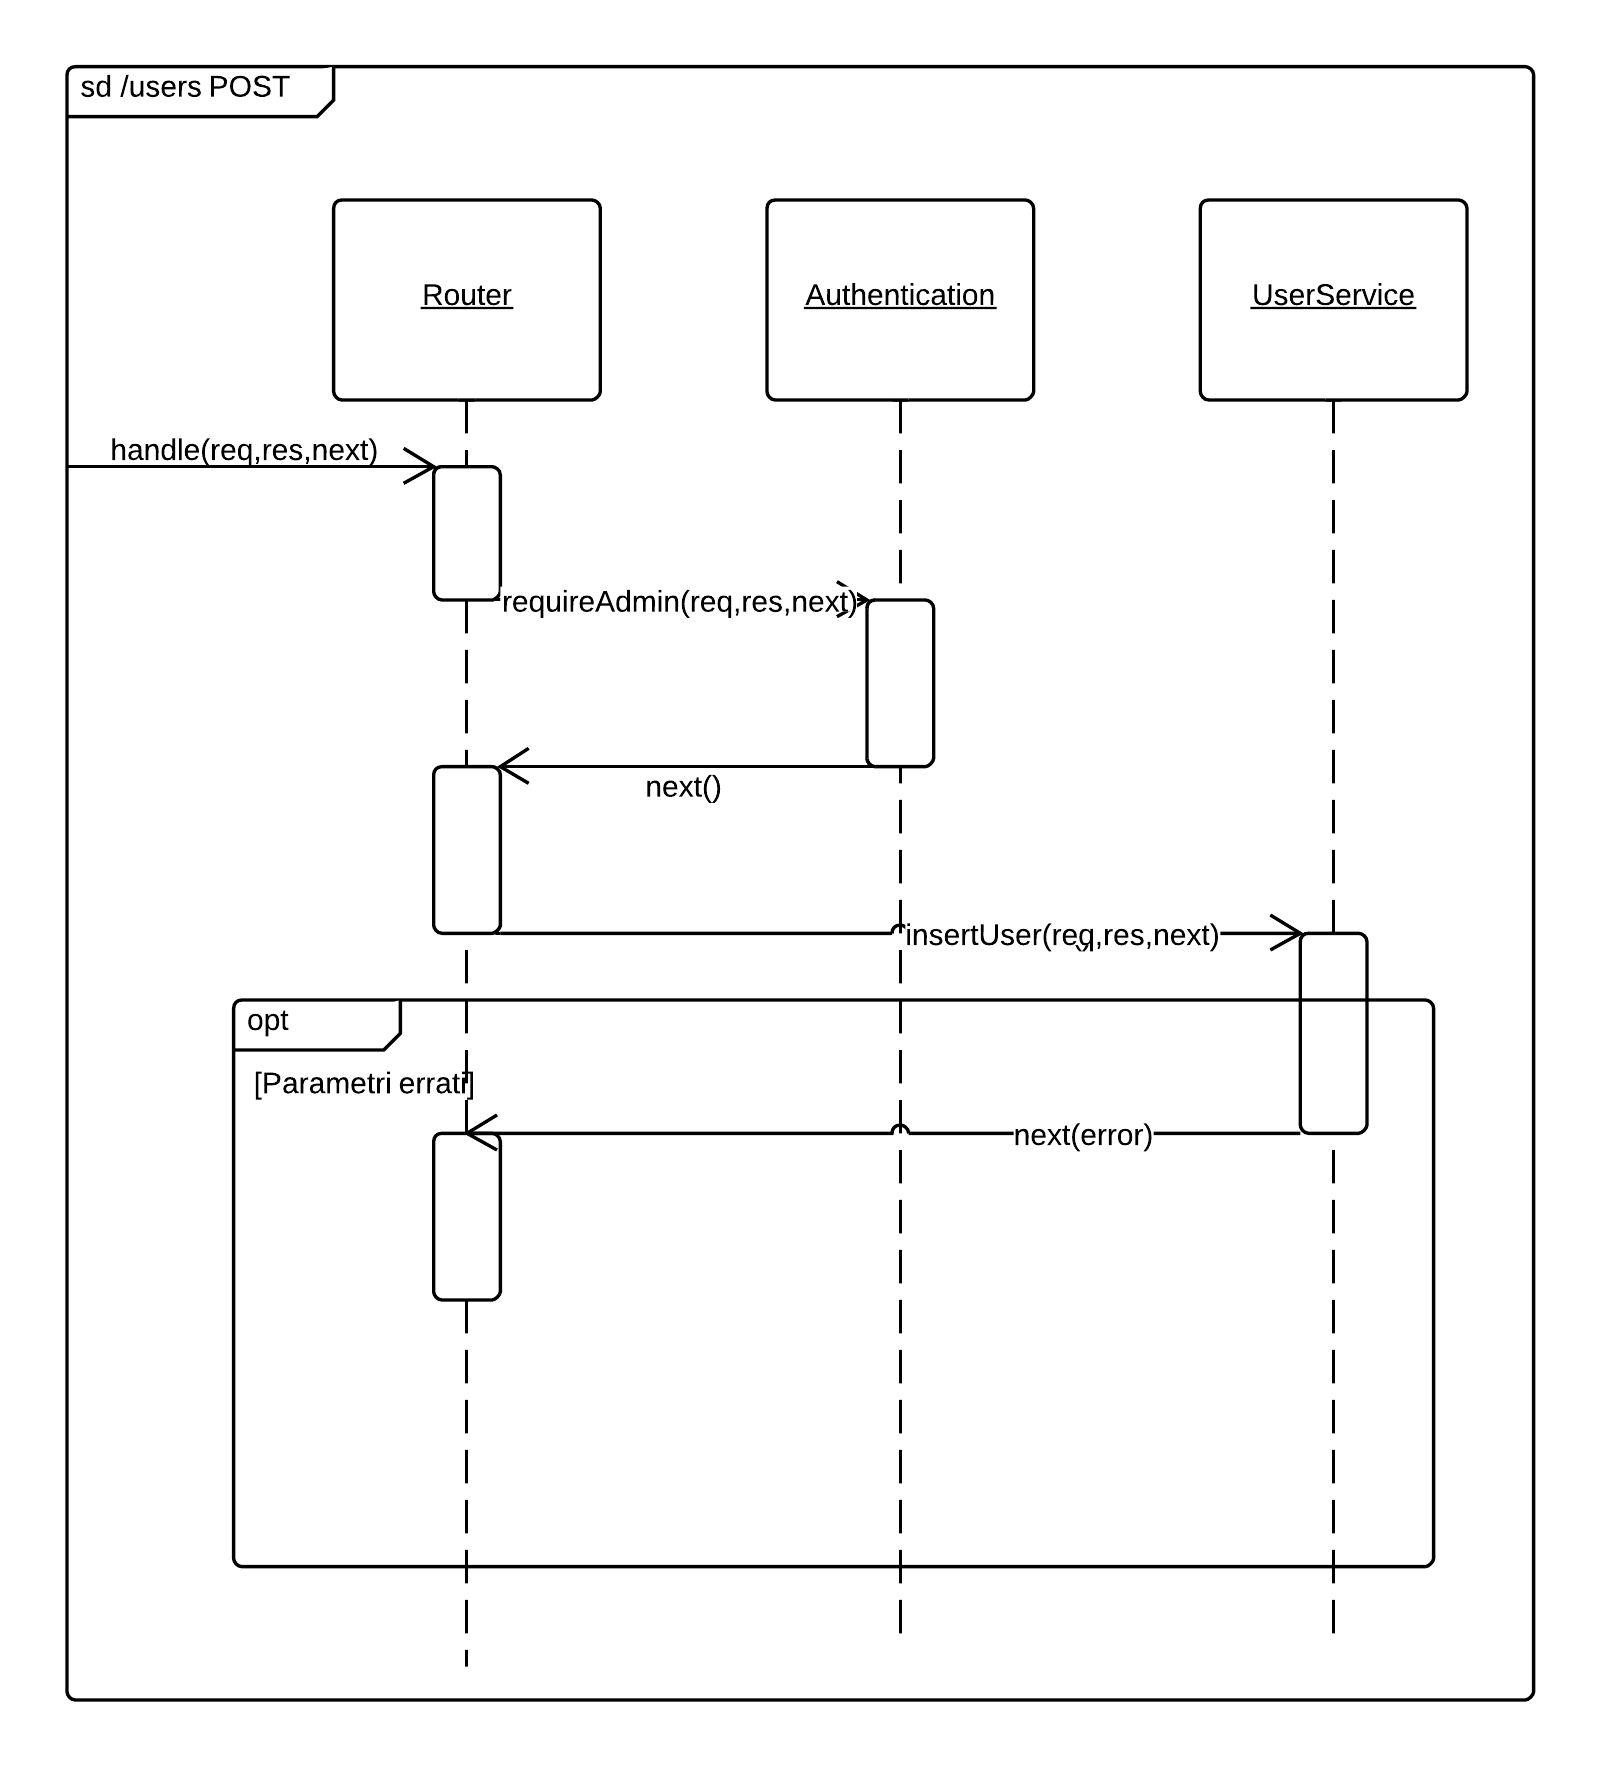
\includegraphics[scale=0.20]{uml/scenari/Users POST.png} 
		\caption{Richiesta POST /users}
	\end{center} 
\end{figure}

\pagebreak
\subsubsection{Richiesta GET /users/\{user id\}} 
Lo scenario rappresenta una richiesta GET di una risorsa User id, vengono verificati i permessi attraverso \emph{requireAdmin} che passa il controllo a \emph{getUser} dandogli come attributo l'id dell'user da restituire.
Nell'opzione che l'id dell'user sia errato, non corrispondendo a nessun user esistente, verrà richiamata una next(error).
\begin{figure}[H]
	\begin{center} 
		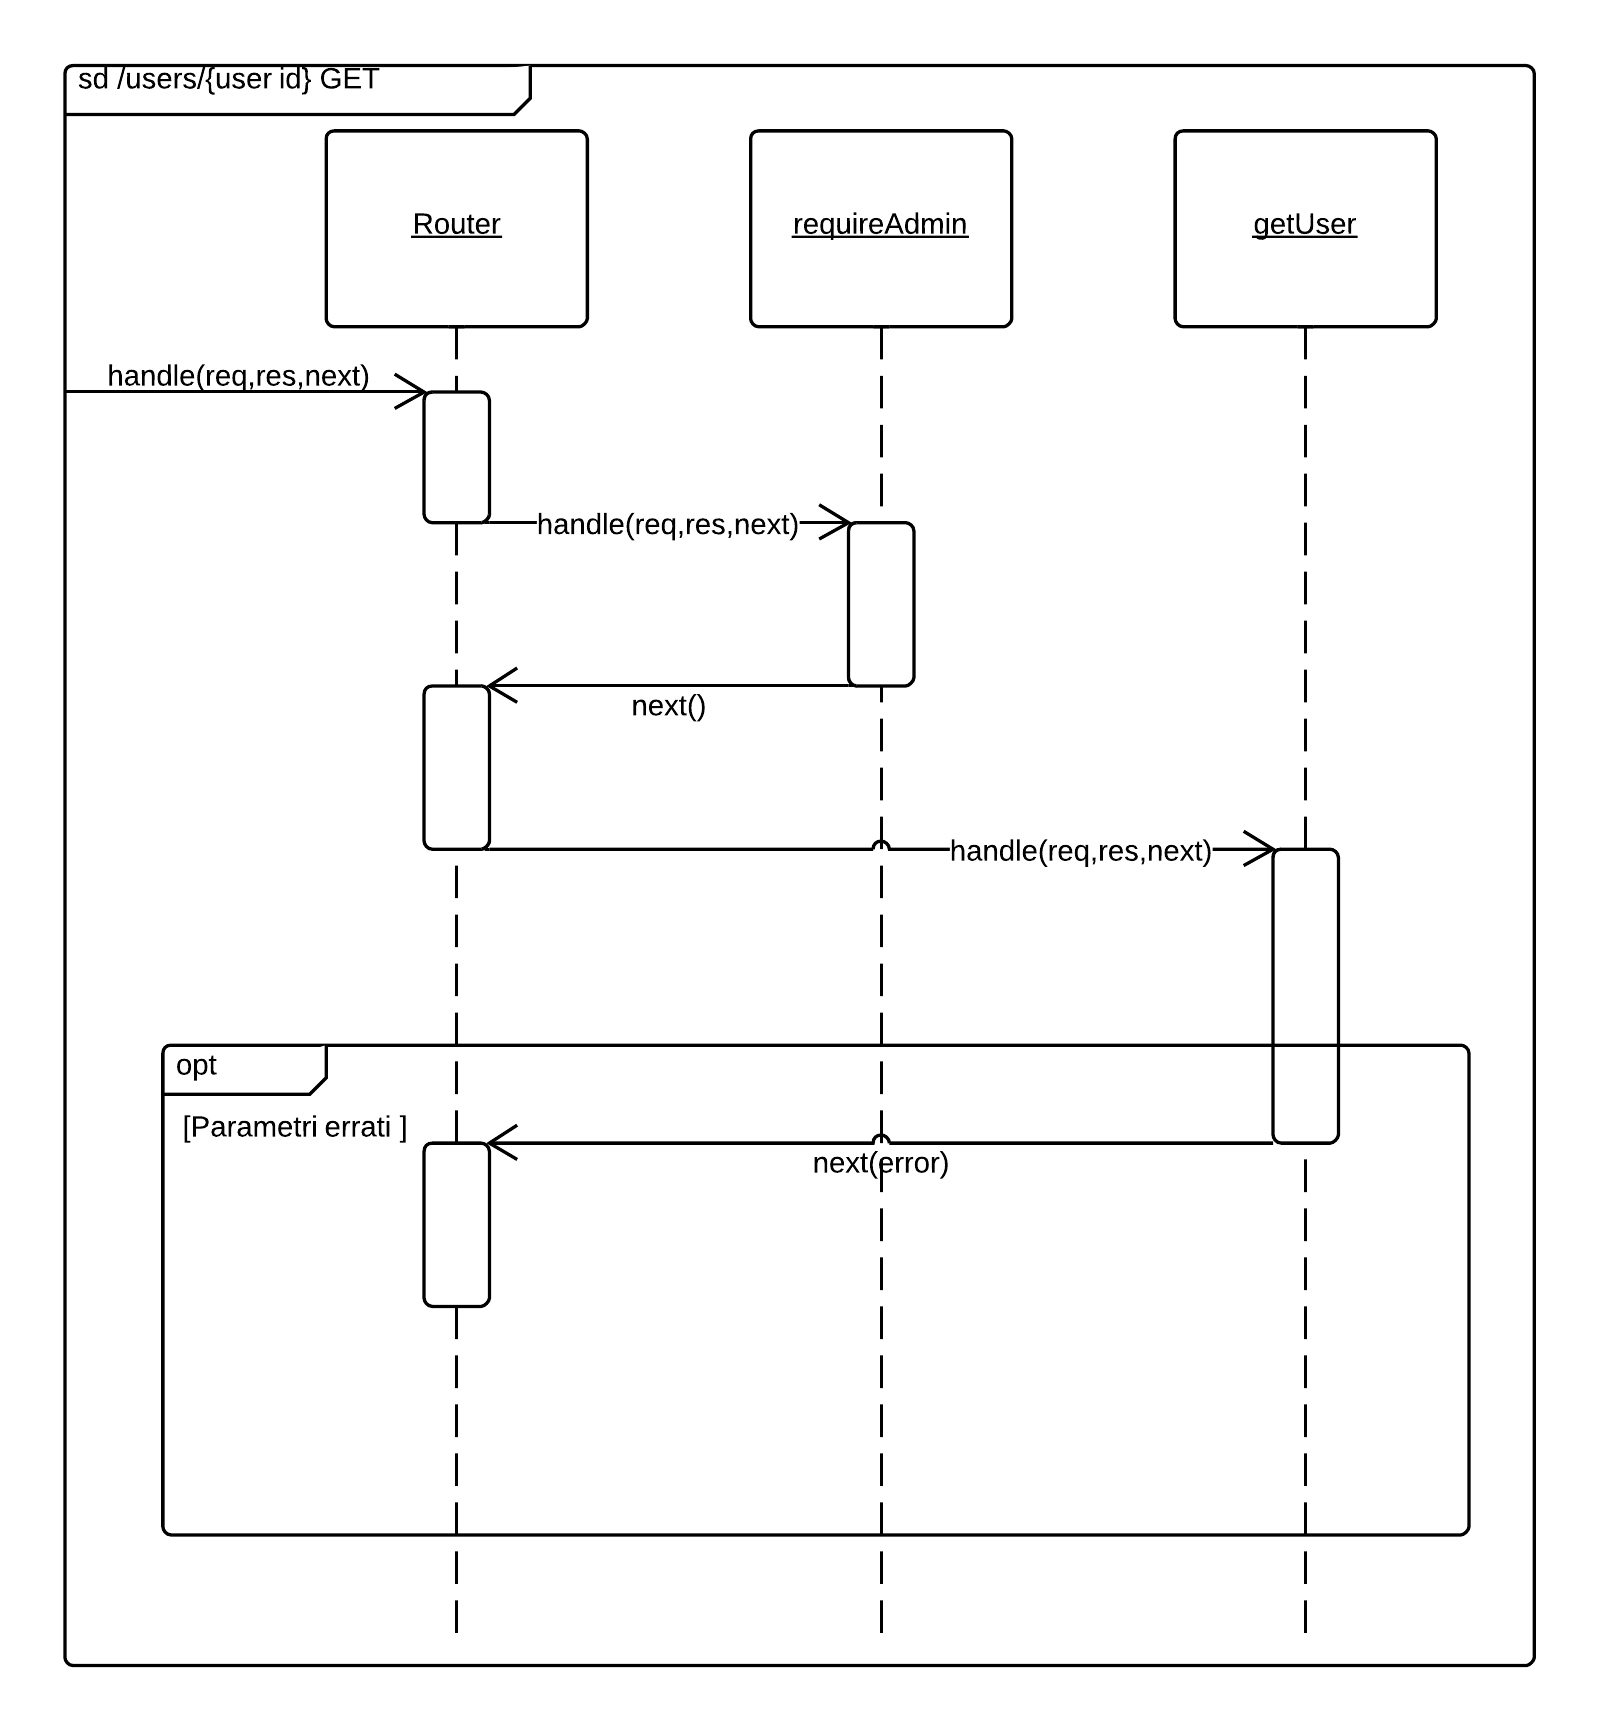
\includegraphics[scale=0.20]{uml/scenari/Users Id GET.png} 
		\caption{Richiesta GET /users/\{user id\}}
	\end{center} 
\end{figure}

\pagebreak
\subsubsection{Richiesta PUT /users/\{user id\}} 
Nel seguente diagramma di sequenza viene rappresentato lo scenario di una richiesta PUT per la risorsa User id nel quale \emph{requireAdmin} non restituisce un errore e passa il controllo a \emph{editUser} che gestisce la richiesta di modifica dati dell'user corrispondente all'userId che gli è stato passato come attributo.
\emph{EditUser} verifica inoltre che l'userId passatogli come attributo non corrisponda all'id dello stesso user che ha effettuato la richiesta o corrisponda ad un id di un superAdmin e controlla che i parametri passati non siano errati, altrimenti risponderà con errore.
\begin{figure}[H]
	\begin{center} 
		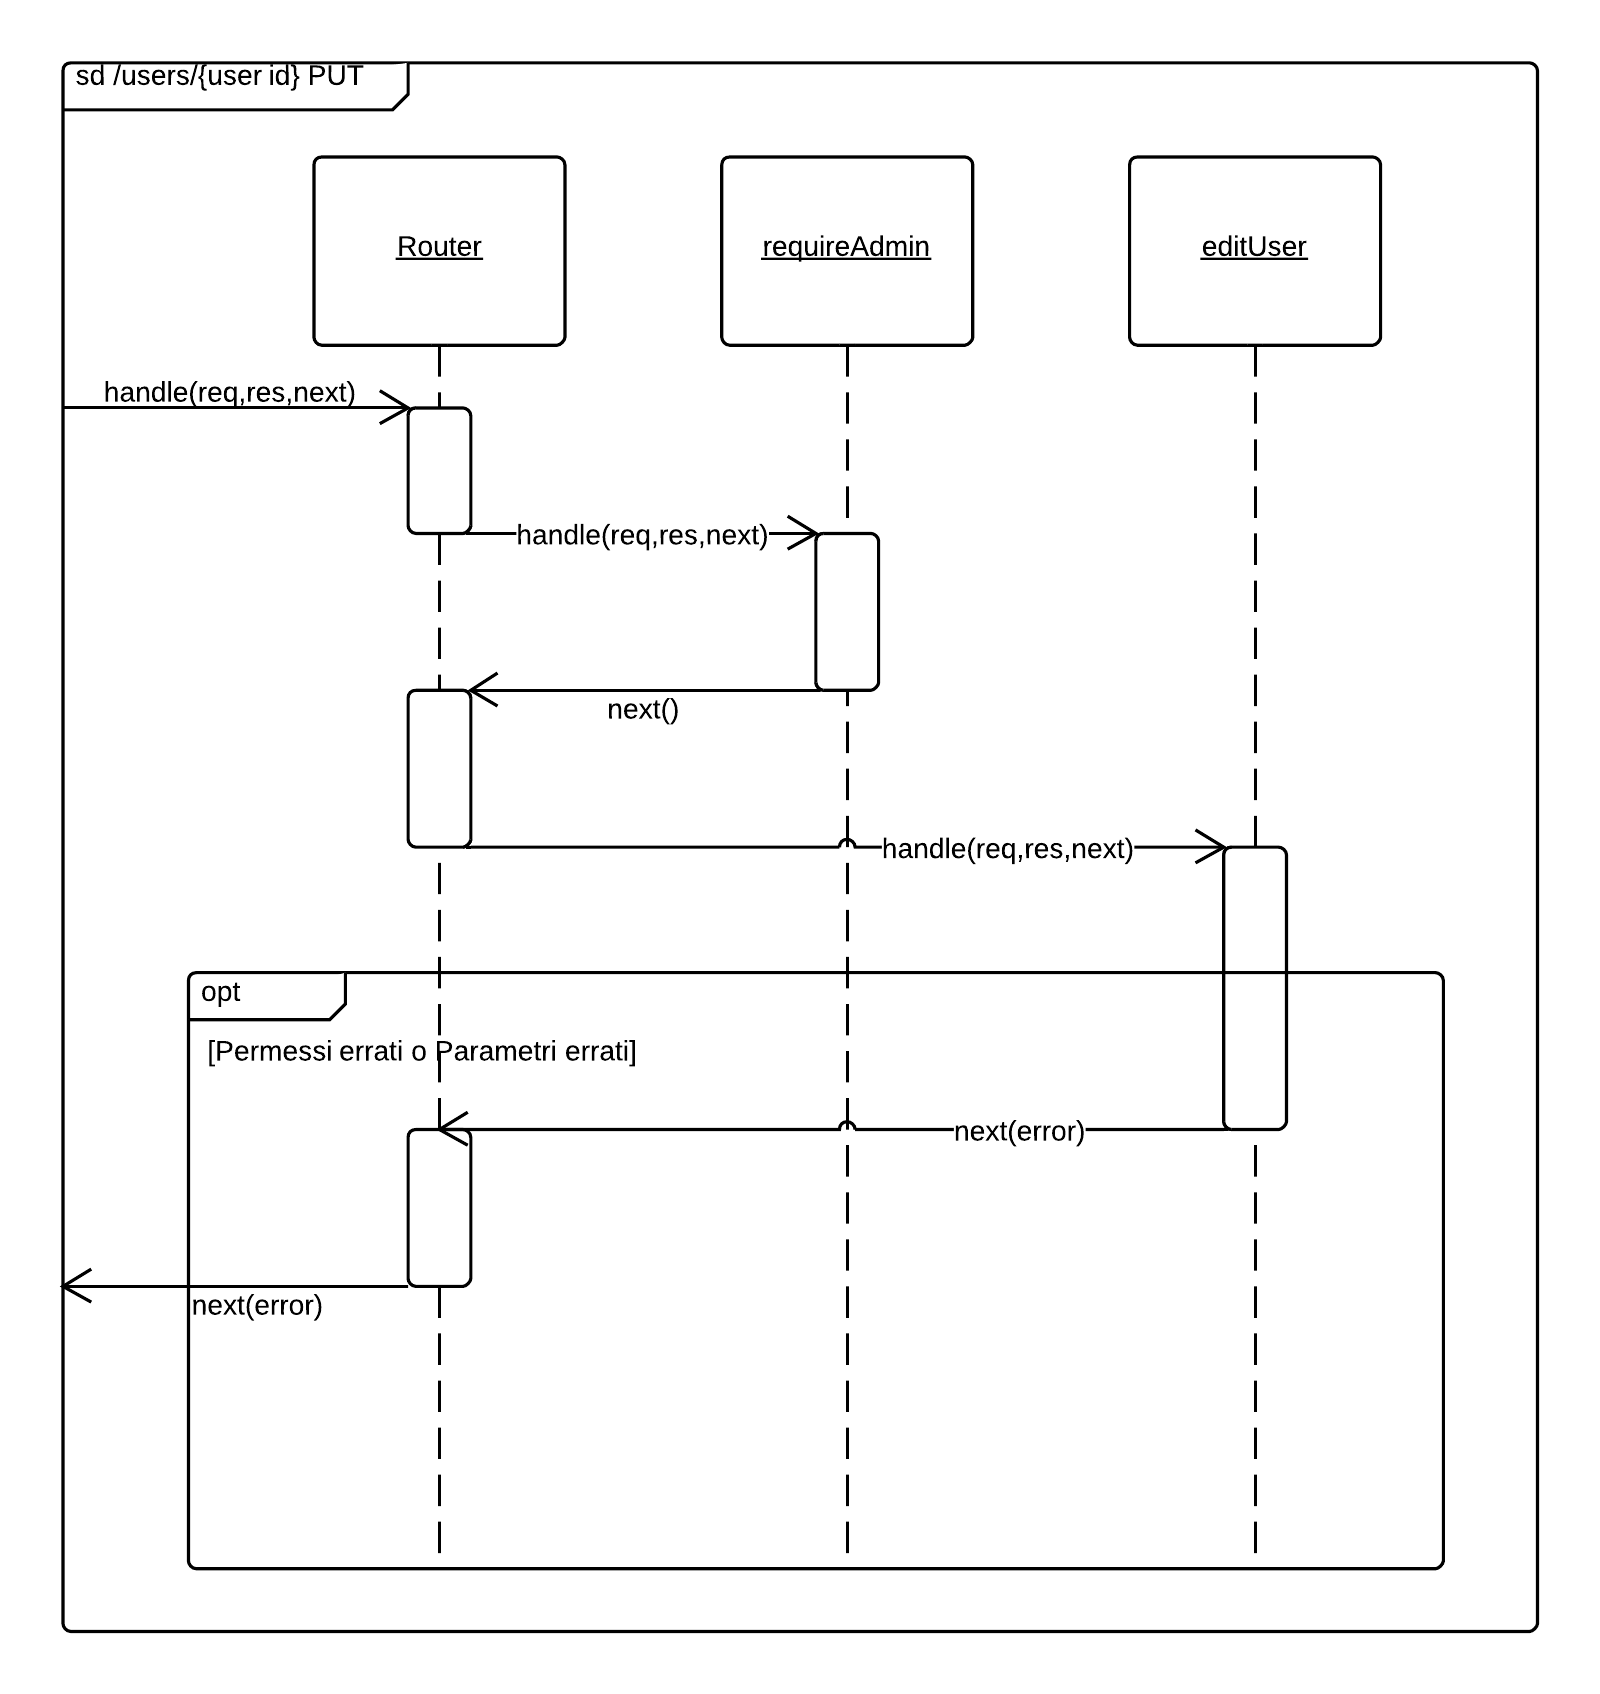
\includegraphics[scale=0.20]{uml/scenari/Users Id PUT.png} 
		\caption{Richiesta PUT /users/\{user id\}}
	\end{center} 
\end{figure}

\pagebreak
\subsubsection{Richiesta DELETE /users/\{user id\}} 
Il diagramma di sequenza rappresenta lo scenario di una richiesta DELETE per la risorsa user id, \emph{requireAdmin} non restituisce un errore e la richiesta viene gestita da \emph{deleteUser} per procede con l'eliminazione dell'user cui id gli è stato passato come attributo.
Nell'opzione che l'id passatogli corrisponda all'id dell'utente che ha effettuato la richiesta o ad un id di un superAdmin, \emph{deleteUser} restituisce un next(error). Il controller si preoccupa inoltre di verificare che i parametri siano corretti.
\begin{figure}[H]
	\begin{center} 
		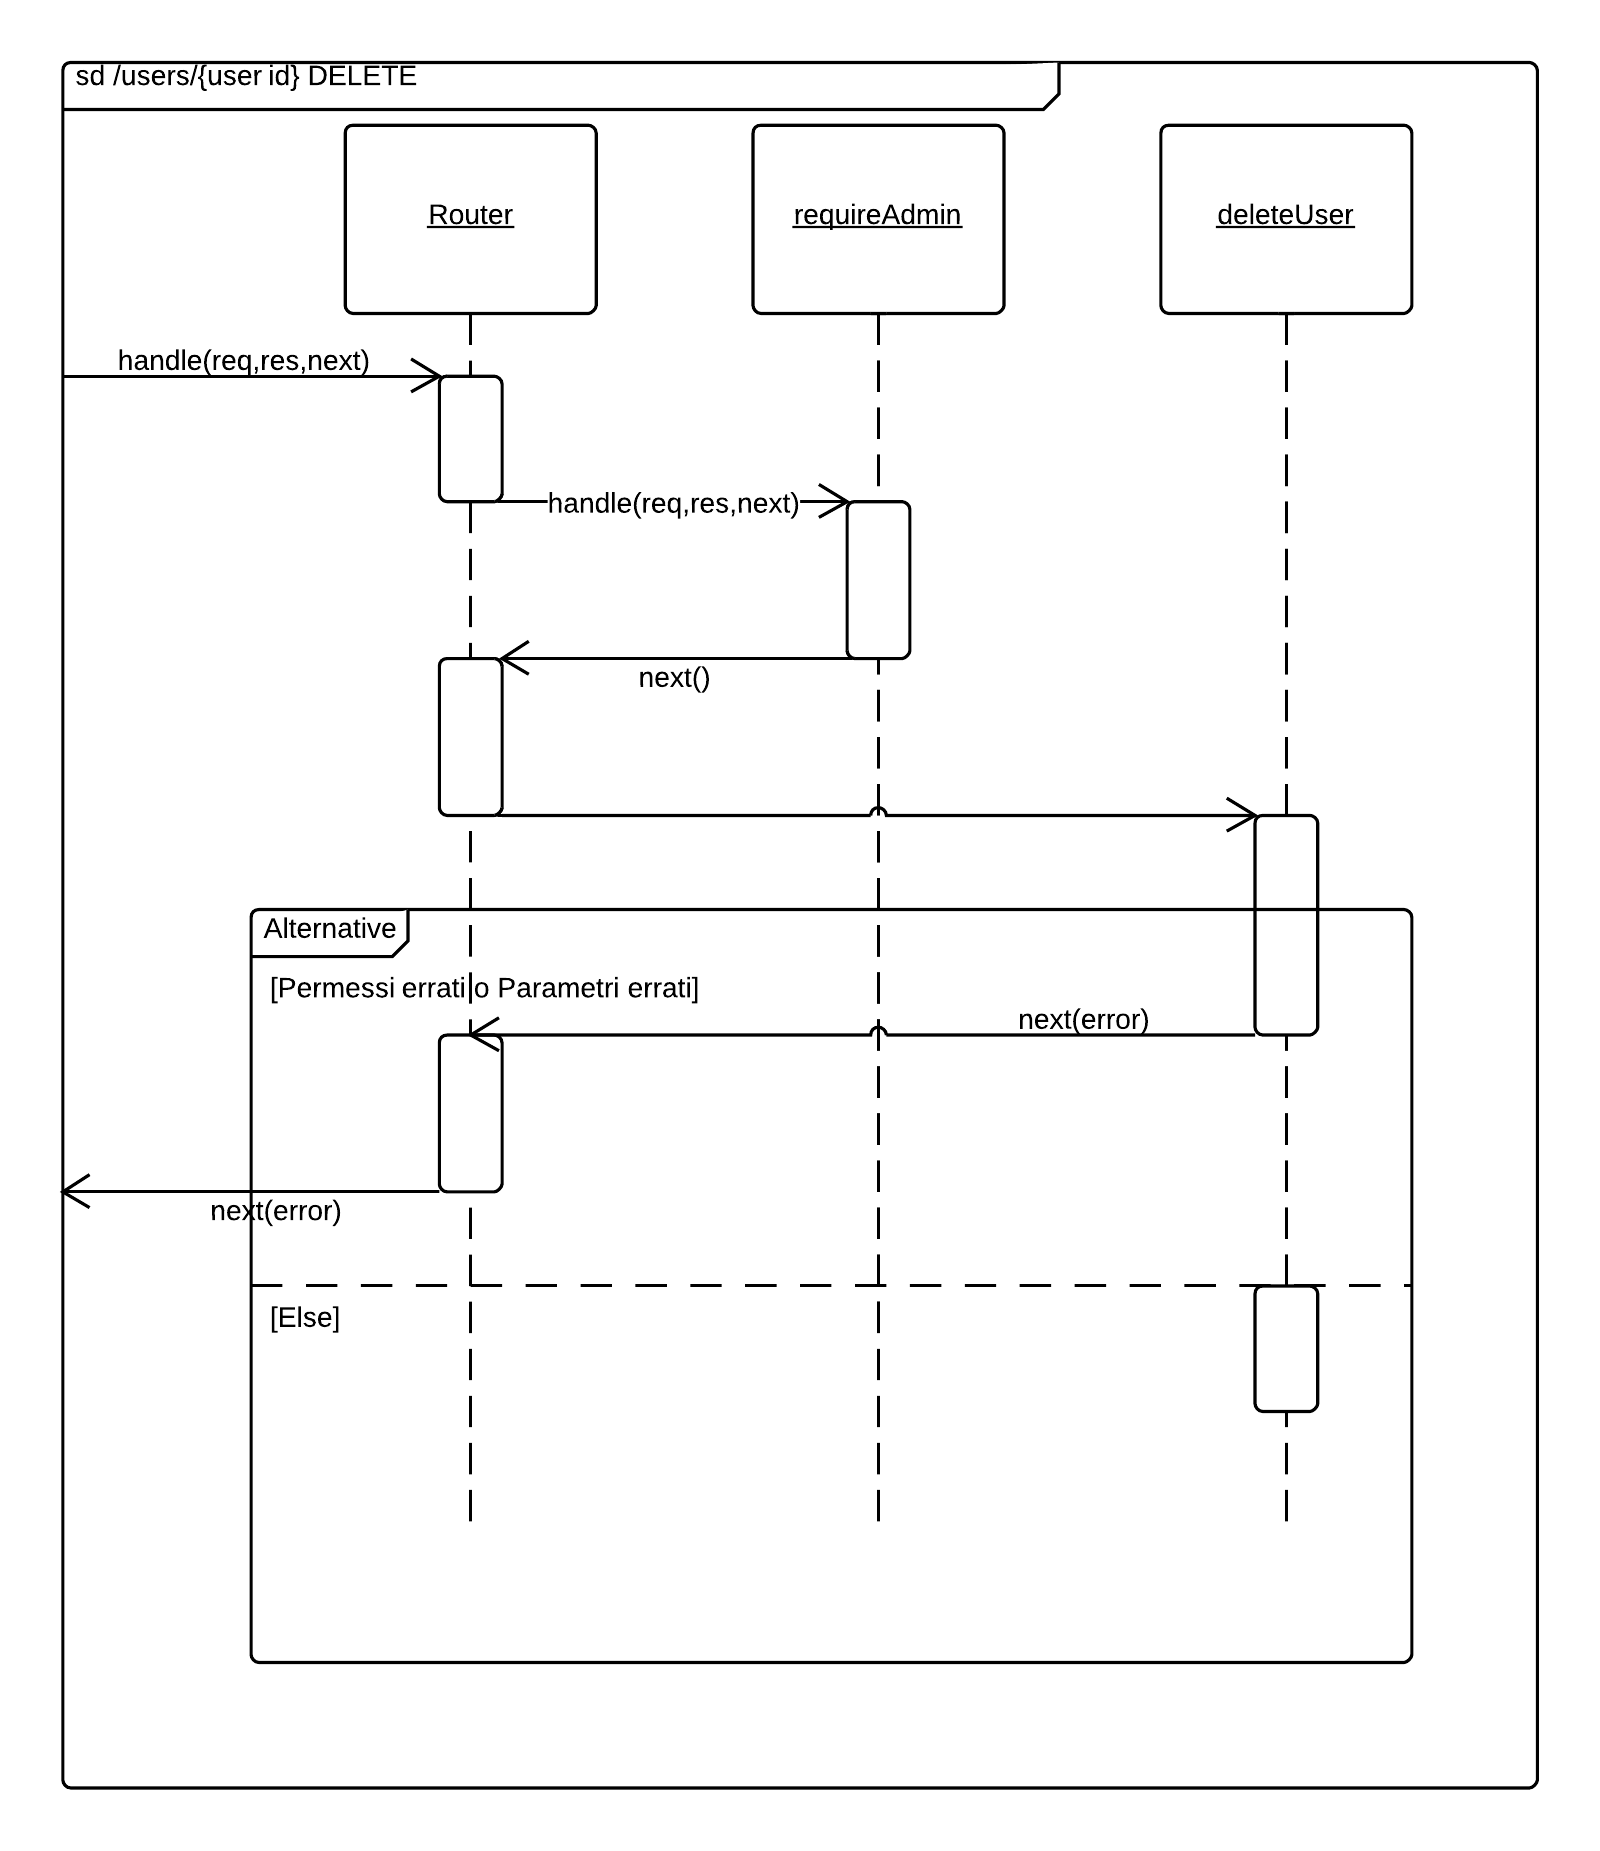
\includegraphics[scale=0.20]{uml/scenari/Users Id DELETE.png} 
		\caption{Richiesta DELETE /users/\{user id\}}
	\end{center} 
\end{figure}

\pagebreak
\subsubsection{Richiesta GET /collection} 
Il diagramma seguente rappresenta lo scenario di una richiesta GET per la risorsa collection, il controller \emph{requireLogged} innescherà la chiamata del successivo controller \emph{listCollection} che gestirà la richiesta di restituzione della lista di \glossario{Collection}.
\begin{figure}[H]
	\begin{center} 
		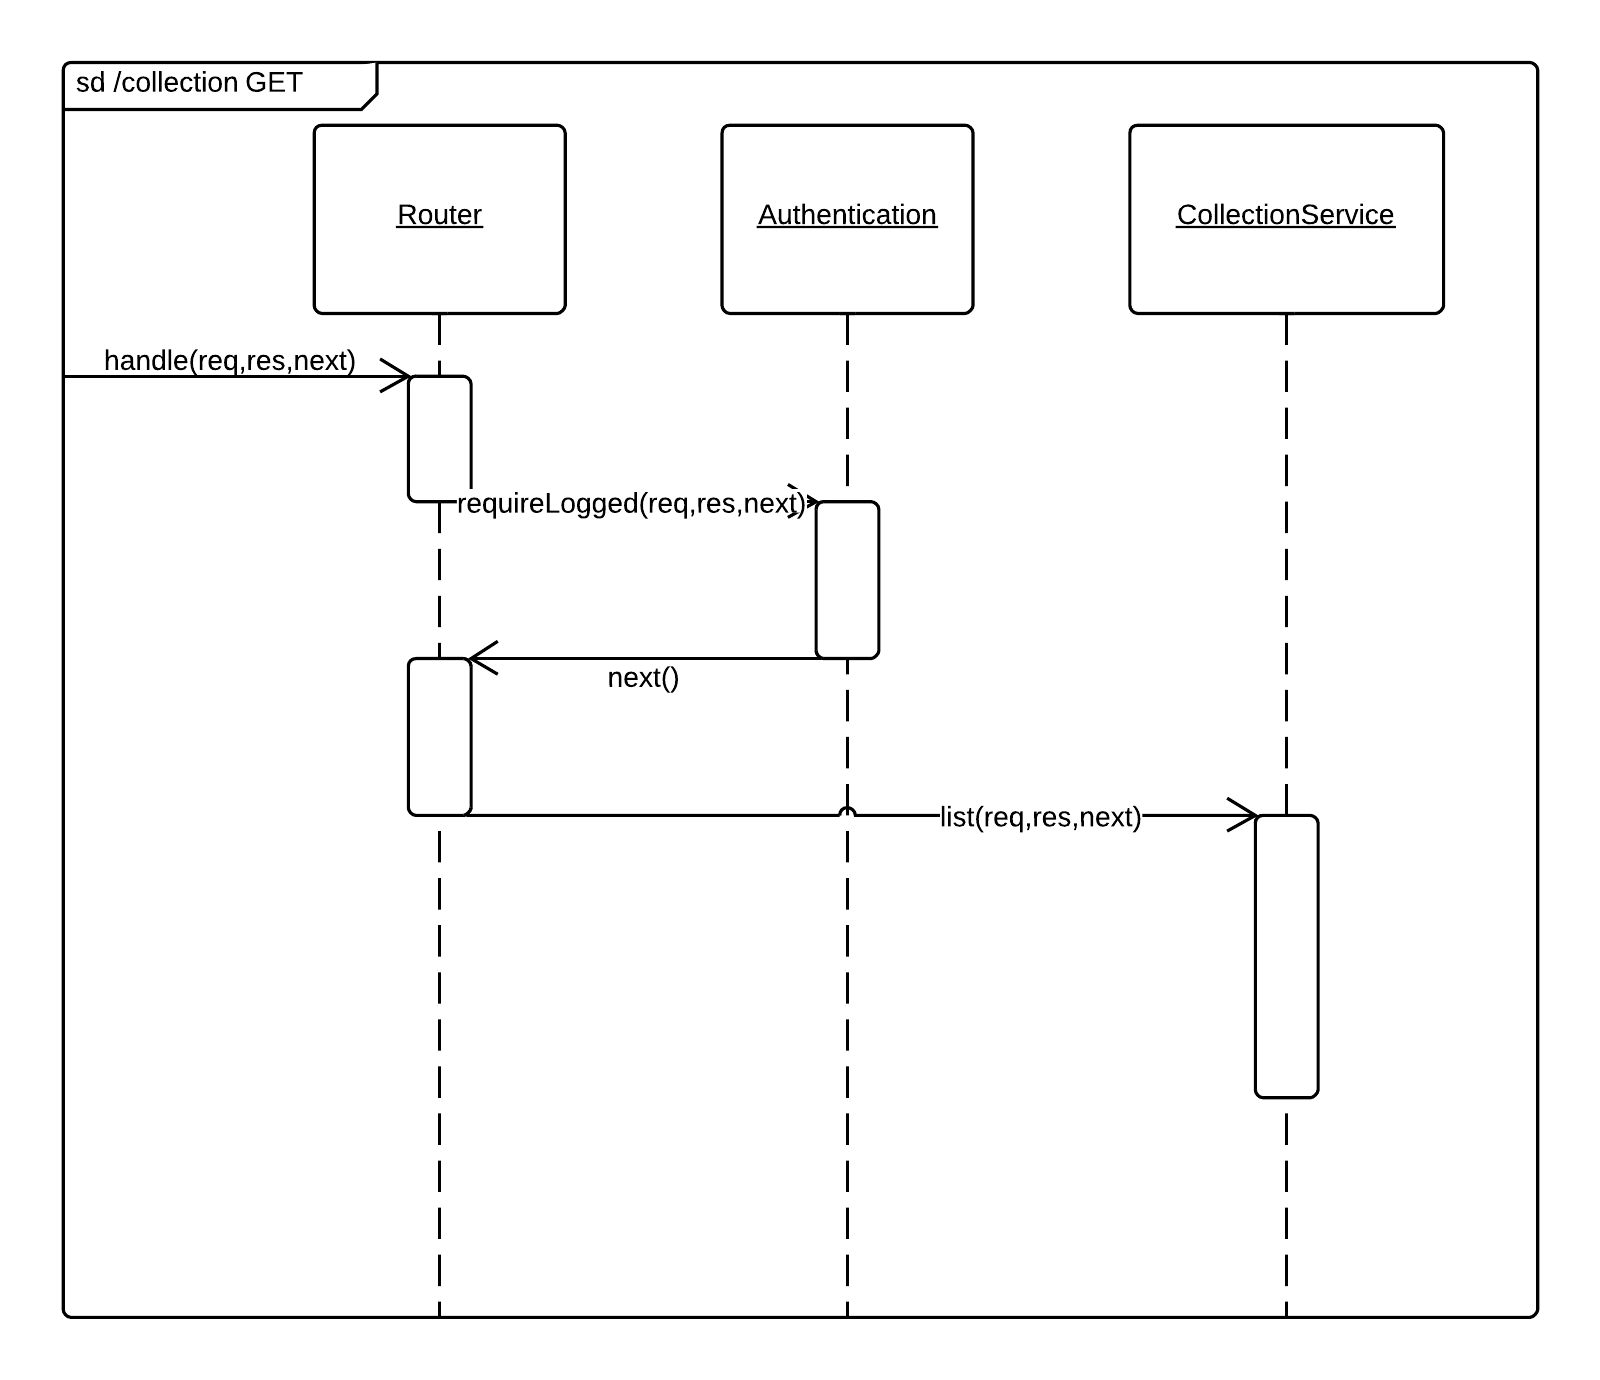
\includegraphics[scale=0.20]{uml/scenari/Collection GET.png} 
		\caption{Richiesta GET /collection}
	\end{center} 
\end{figure}

\pagebreak
\subsubsection{Richiesta GET /collection/\{collection name\}} 
Il diagramma seguente rappresenta lo scenario di una richiesta GET per la risorsa collection Name, il controller \emph{requireLogged} innescherà la chiamata del successivo controller \emph{indexPage} al quale verrà passato come parametro l'id della \glossario{Collection} per la restituzione dell'index page corrispondente. \\ 
Nell'opzione che l'id sia errato il controller chiamerà la callback passandogli la descrizione dell'errore come parametro.
\begin{figure}[H]
	\begin{center} 
		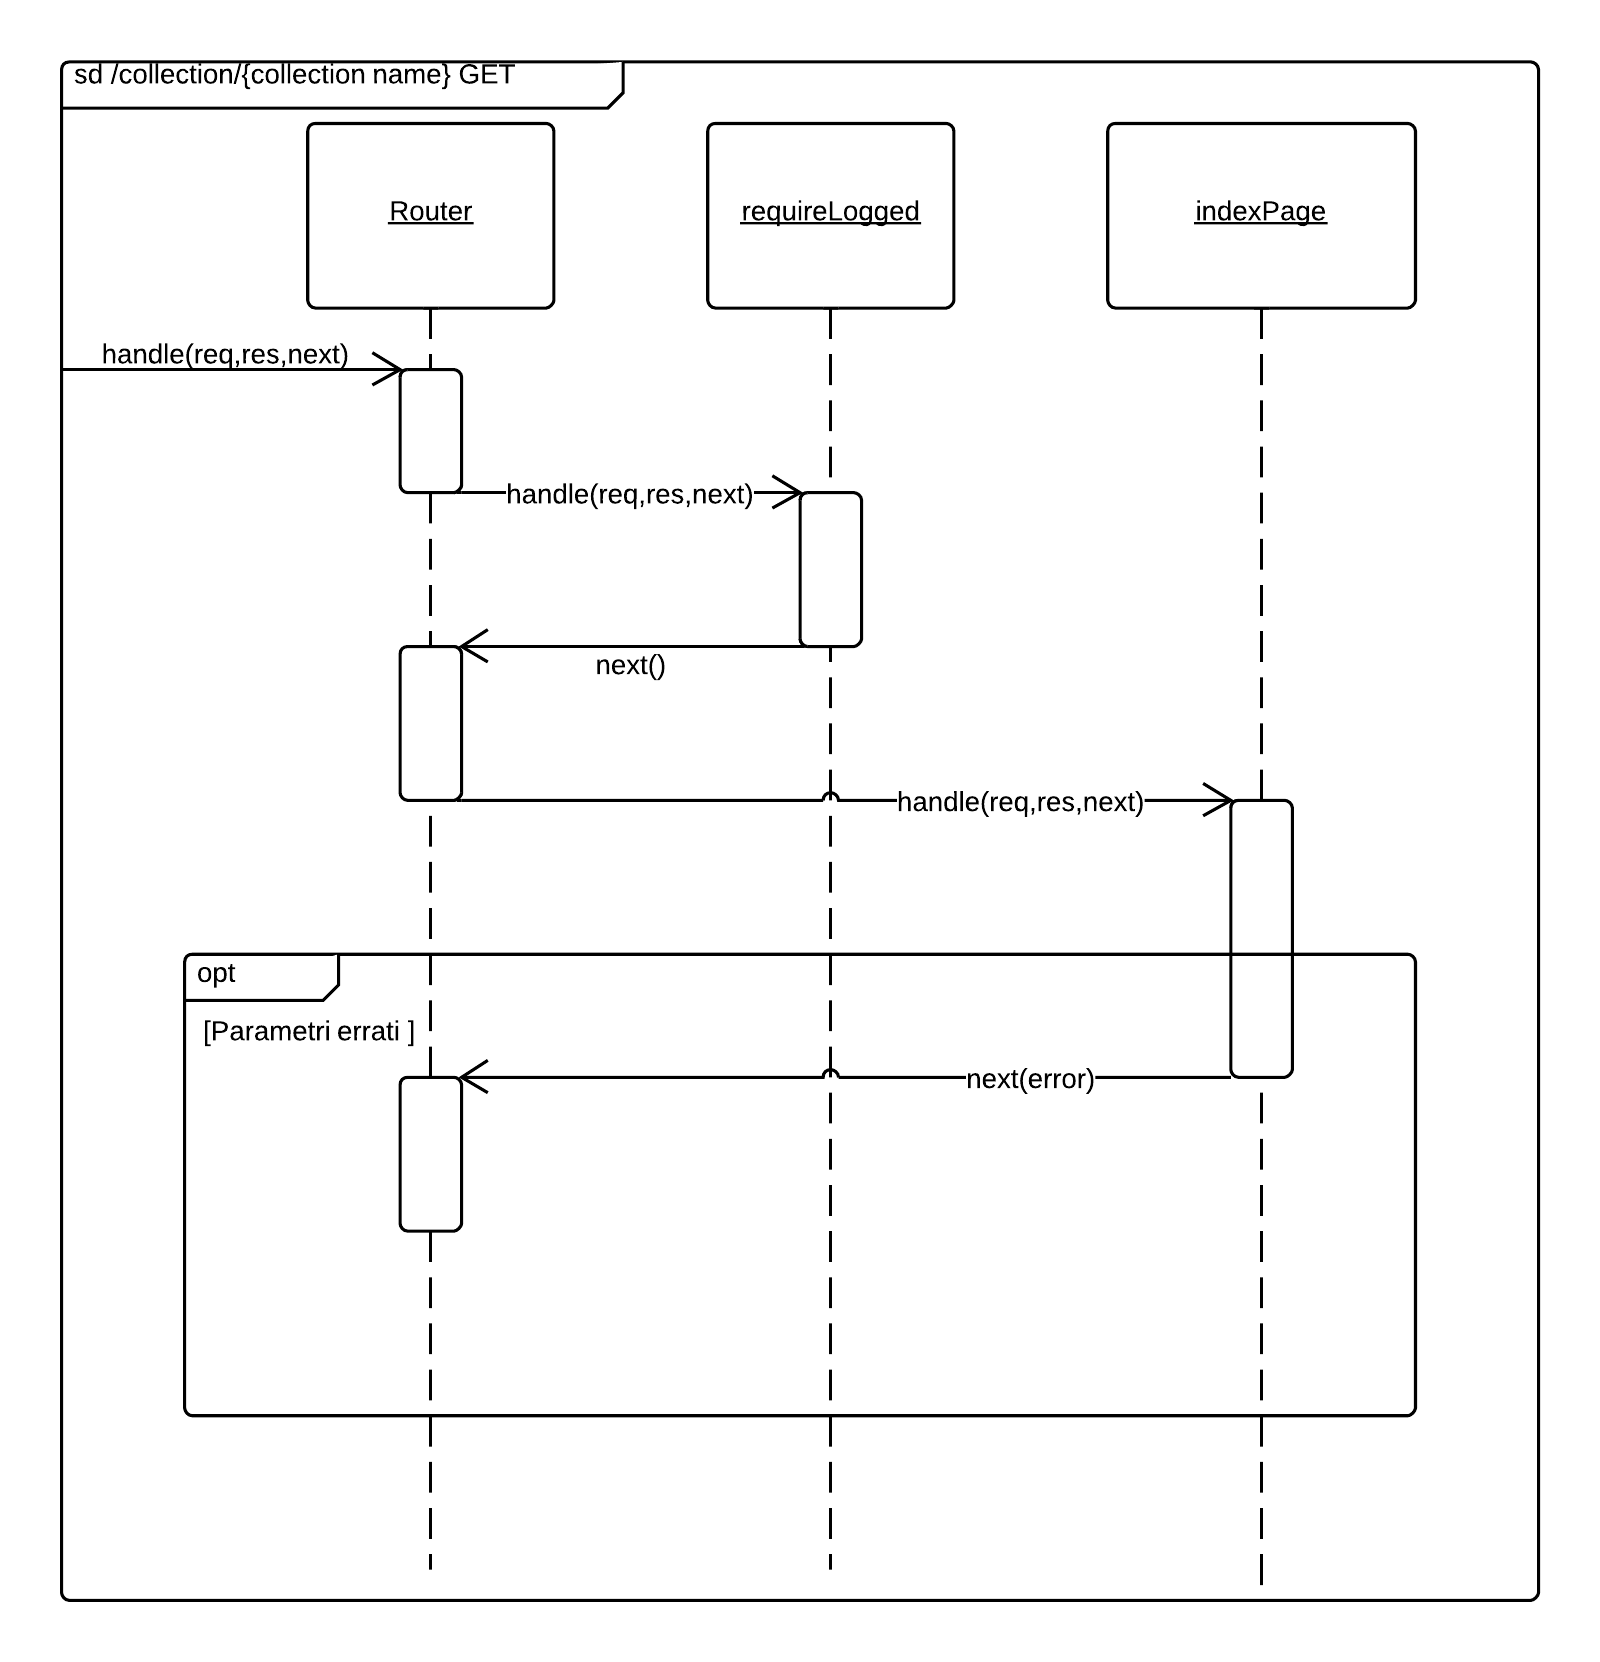
\includegraphics[scale=0.20]{uml/scenari/Collection Name GET.png} 
		\caption{Richiesta GET /collection/\{collection name\}}
	\end{center} 
\end{figure}

\pagebreak
\subsubsection{Richiesta GET /collection/\{collection name\}/\{document id\}} 
Il diagramma di sequenza rappresenta lo scenario di una richiesta GET per la risorsa collection name document, nel quale al controller \emph{showpage} viene passato l'id del document di cui mostrare la show page.
Nell'opzione l'id sia errato, non corrispondendo ad un \glossario{Document} valido, \emph{showpage} restituisce una next(error).
\begin{figure}[H]
	\begin{center} 
		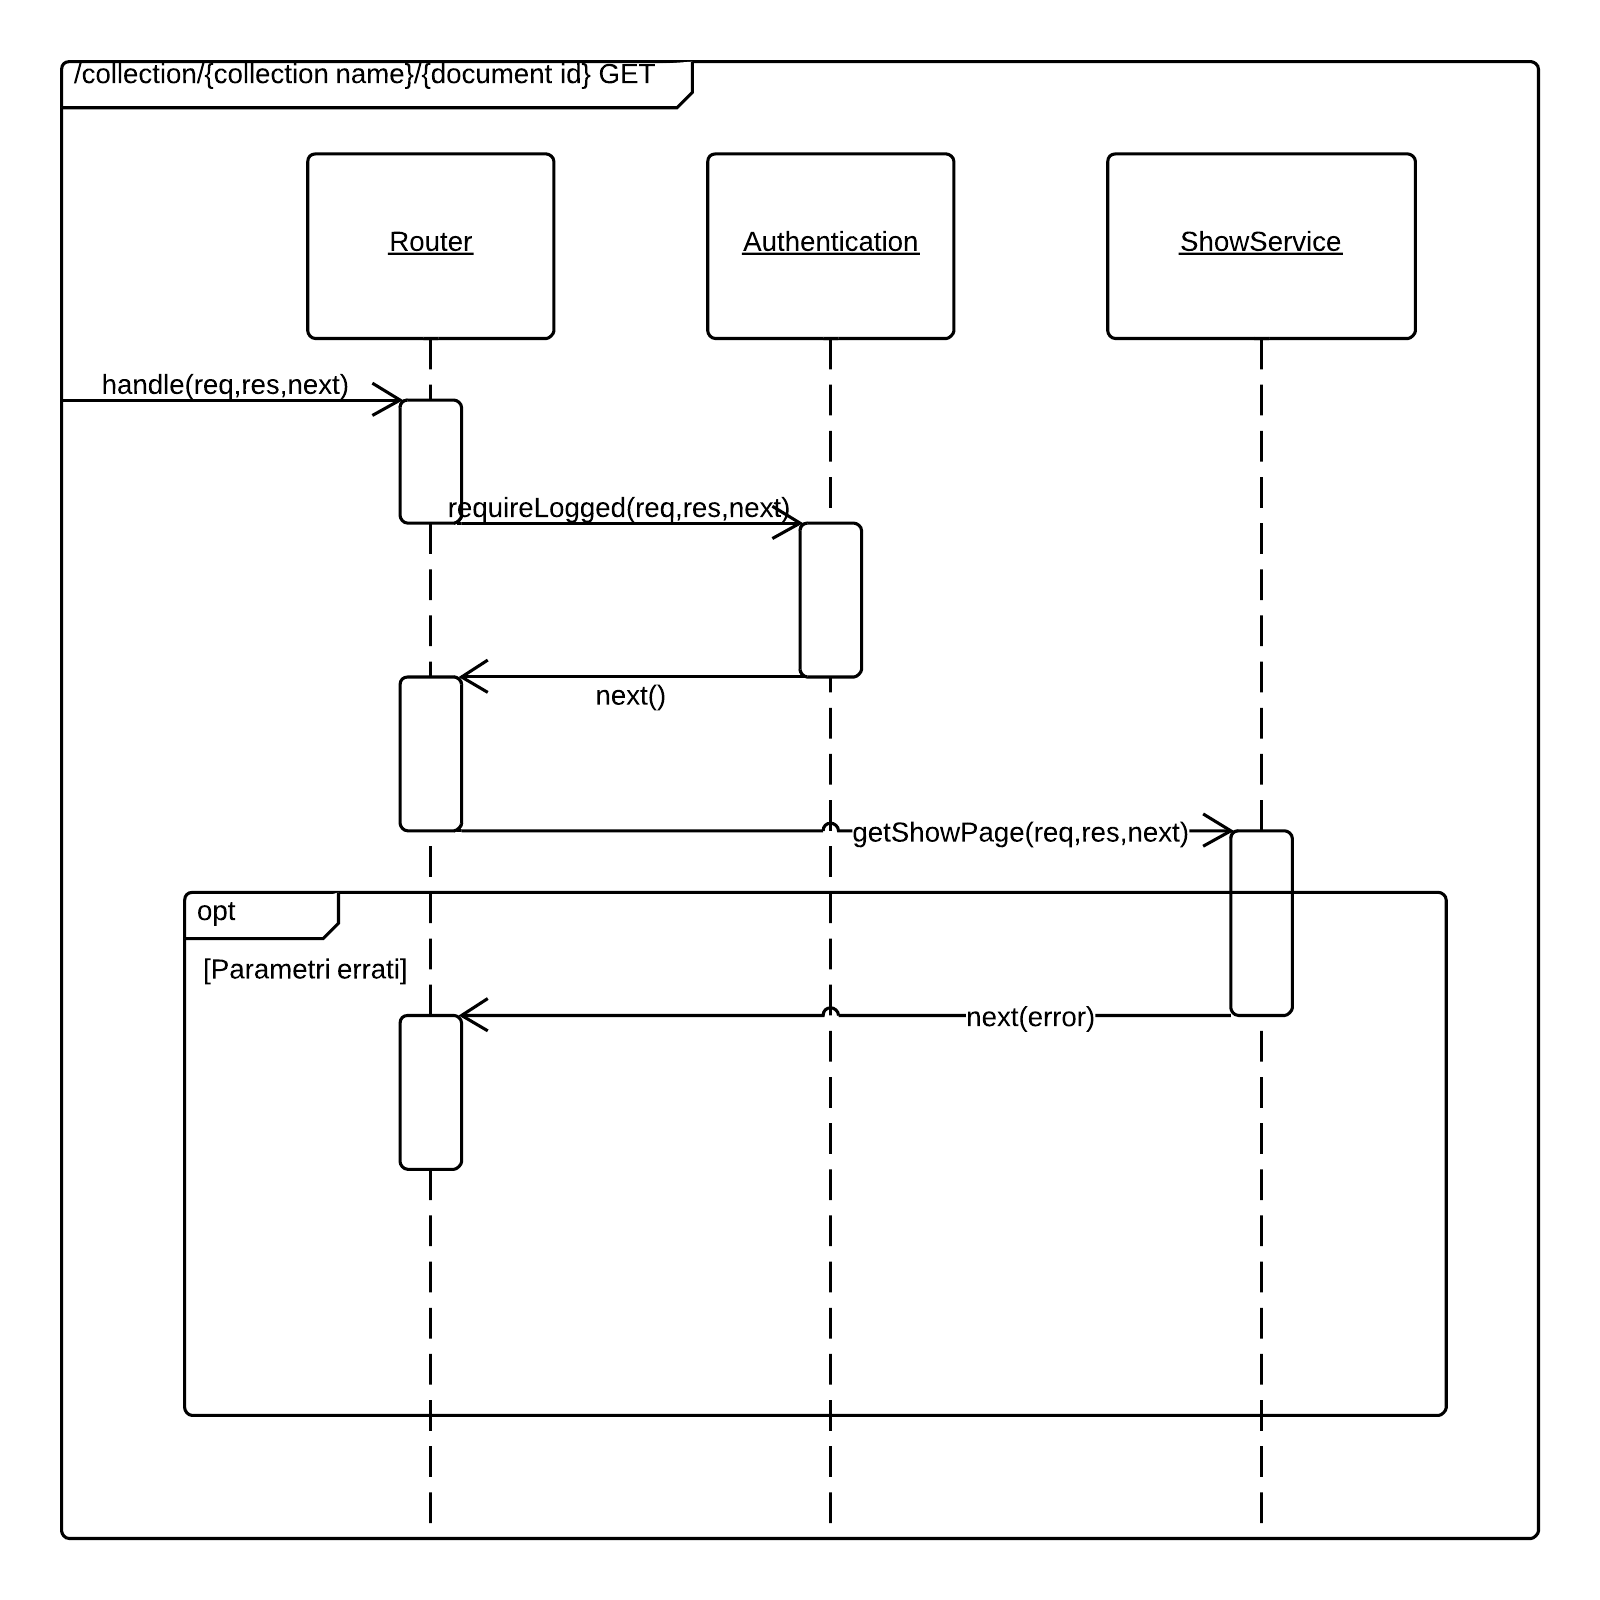
\includegraphics[scale=0.20]{uml/scenari/Collection Name Document GET.png}
		\caption{Richiesta GET /collection/\{collection name\}/\{document id\}}
	\end{center} 
\end{figure}


\pagebreak
\subsubsection{Richiesta DELETE /collection/\{collection name\}/\{document id\}}
Il seguente scenario rappresenta la richiesta DELETE per una risorsa Collection name document, dopo che i permessi sono stati verificati il controllo è passato a \emph{deleteDocument} il quale gestirà la richiesta di eliminazione del document il cui id gli è stato passato come parametro. Se l'id è errato, verrà restituito un errore.
\begin{figure}[H]
	\begin{center} 
		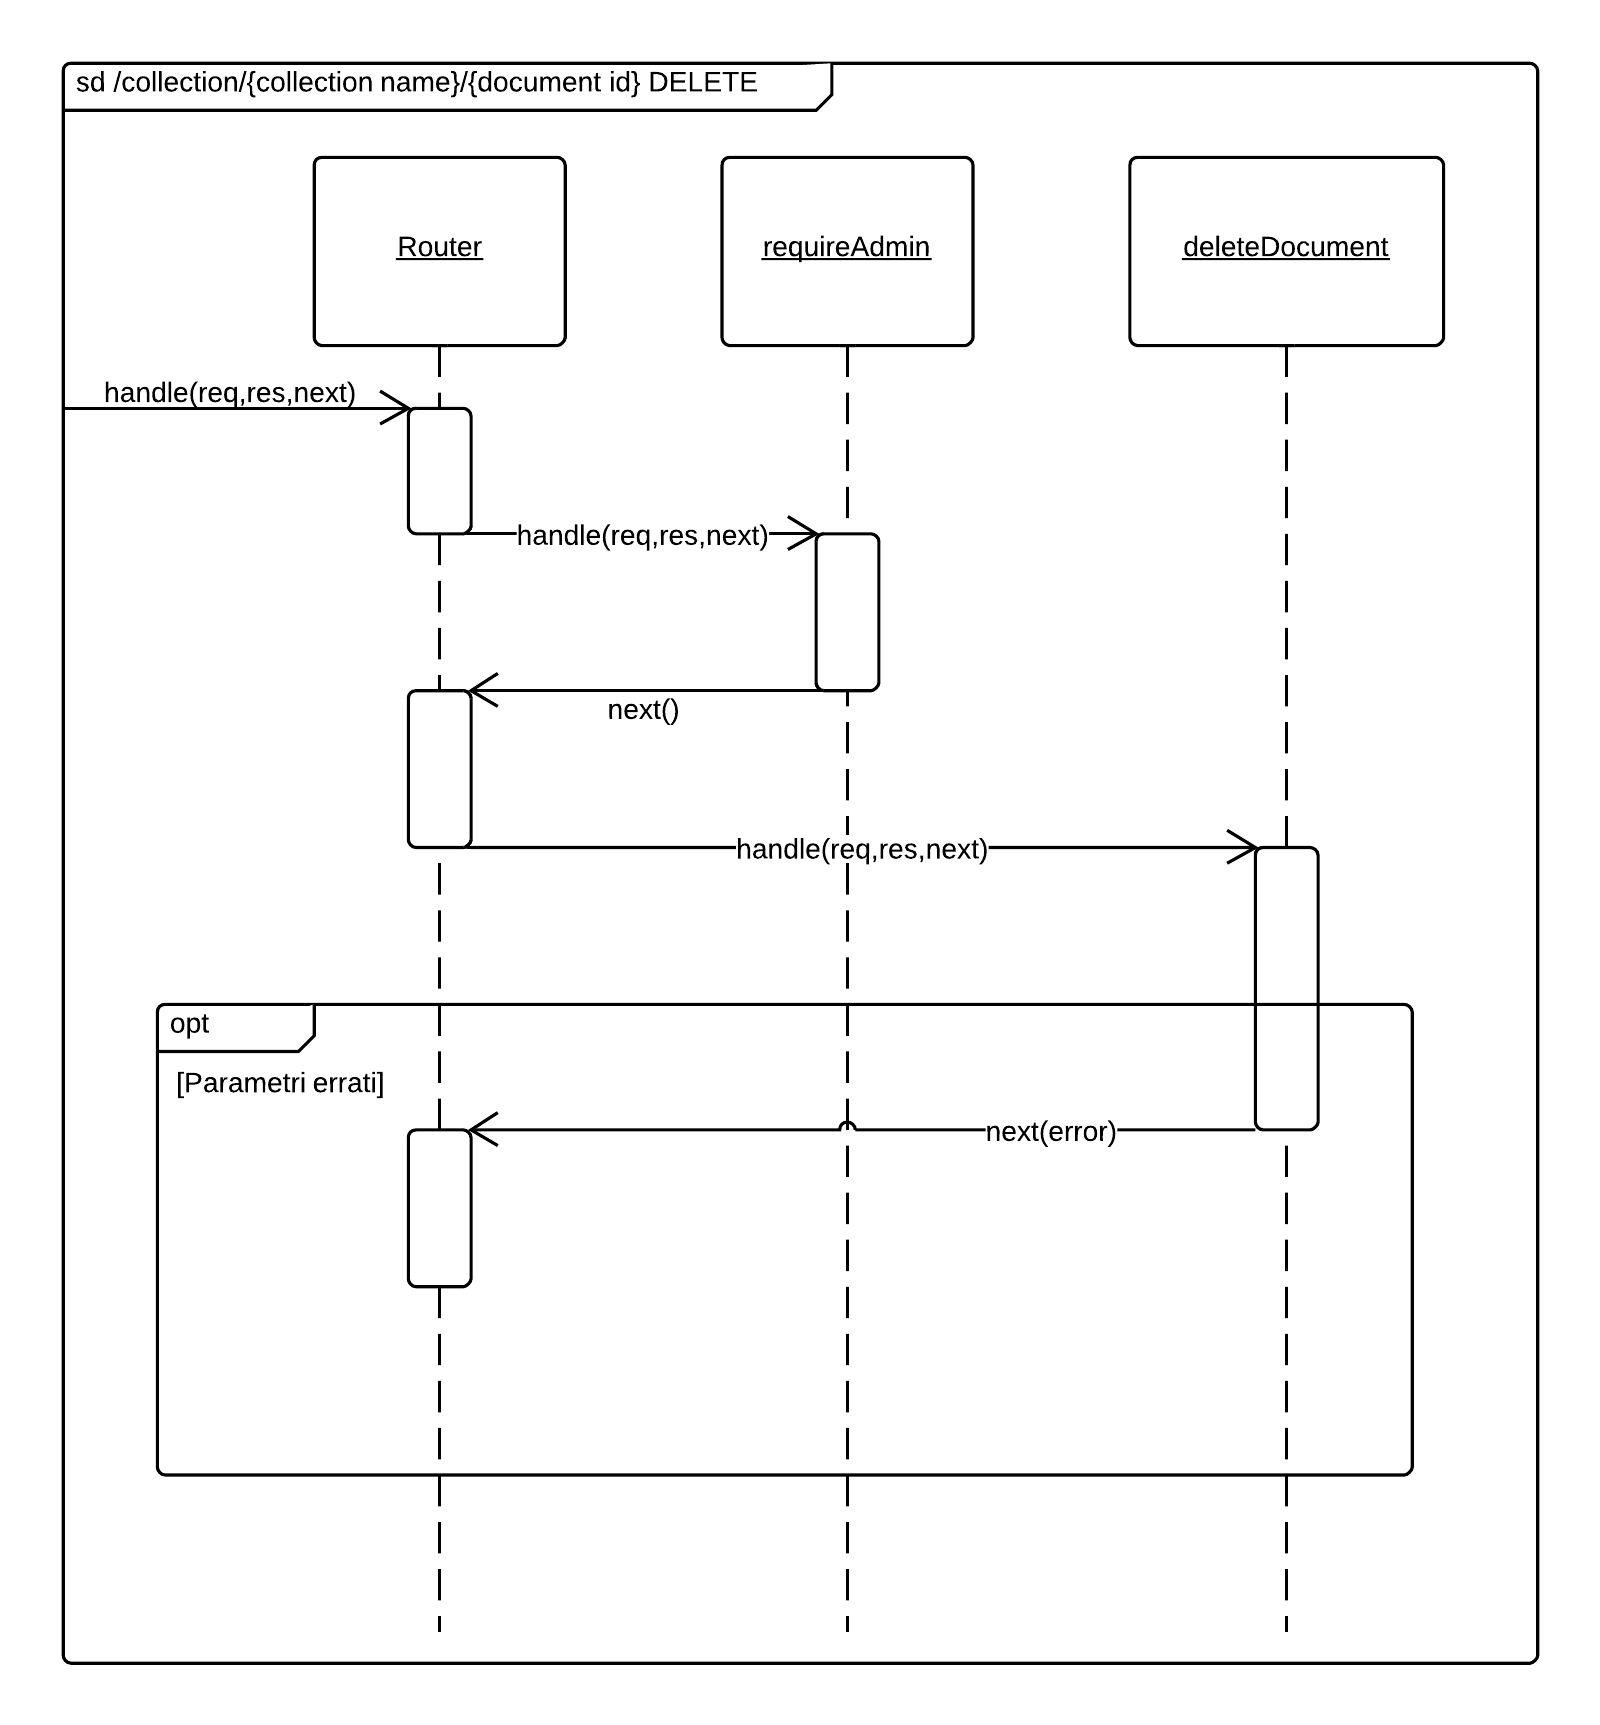
\includegraphics[scale=0.20]{uml/scenari/Collection Name Document DELETE.png} 
		\caption{Richiesta DELETE /collection/\{collection name\}/\{document id\}}
	\end{center} 
\end{figure}

\clearpage
\subsection{Descrizione librerie aggiuntive}

Vengono di seguito descritte le librerie aggiuntive utilizzate dal Back-end che corrispondono nei diagrammi precedenti ai packages colorati. La scelta è stata effettuata cercando di valutare la diffusione, il livello di stabilità, l'assenza di errori noti.

\begin{itemize}
 \item \textbf{Passport:} è un middleware di autenticazione per \glossario{Node.js}. Estremamente flessibile e modulare, Passport può essere facilmente inserito in qualsiasi applicazione web basata su Express.
 \item \textbf{Passport-local:} è una libreria che permette di autenticare un utente con Passport usando un username e una password.
 \item \textbf{Passport-local-mongoose:} è un plugin per Mongoose che semplifica la costruzione di un sistema di autenticazione con Passport.
 \item \textbf{Nodemailer:} è un modulo che permette di mandare facilmente e-mail con Node.js, tramite \glossario{SMTP}. Supporta anche i caratteri \glossario{unicode}.
 \item \ \textbf{Sweet:} è un modulo che permette di definire macro utilizzando la sintassi del linguaggio Javascript.
\end{itemize}


\section{Front-end}


\subsection{Diagramma dei package}

\subsection{Diagramma delle classi}
\section{Descrizione dei singoli componenti}

% Nell'indice proposto da Tullio c'è:
% a. Tipo, obiettivo e funzione del componente
% b. Relazioni d'uso di altre componenti
% c. Interfacce con e relazioni di uso da altre componenti
% d. Attività svolte e dati trattati
\section{Diagrammi di attività}

Vengono in seguito illustrati i diagrammi di attività prodotti durante la progettazione architetturale, i quali descrivono le iterazioni dell'utente con il sistema \glossario{MaaP}. È stato scelto di dividere i diagrammi in due categorie principali, in modo analogo a quanto fatto nella descrizione dei casi d'uso dell'\textit{Analisi dei requisiti}:

\begin{itemize}

	\item \textbf{Applicazione \glossario{MaaP}}, in cui verranno descritte le iterazioni che un utente può fare all'interno di un'applicazione generata dal \glossario{framework};
	\item \textbf{Framework \glossario{MaaP}}, in cui verrà descritto il modo in cui uno sviluppatore può creare un'applicazione.

\end{itemize}

Inizialmente per ogni categoria verrà fornito uno schema ad alto livello, per poi andare sempre più nel dettaglio tramite sotto-diagrammi più specifici. Per comodità di visualizzazione le attività che verranno \textit{esplose} sono marcate in grassetto. 

Al fine di rendere il diagramma leggibile abbiamo considerato implicito il fatto che un utente possa in qualsiasi momento uscire dall'applicazione \glossario{MaaP}, per esempio chiudendo la finestra del browser.

\subsection{Applicazione MaaP}

Vengono di seguito descritte tutte le iterazioni che un utente può effettuare con un'applicazione generata dal \glossario{framework} \glossario{MaaP}.


\subsubsection{Attività principali}

\begin{figure}[H]
\centering
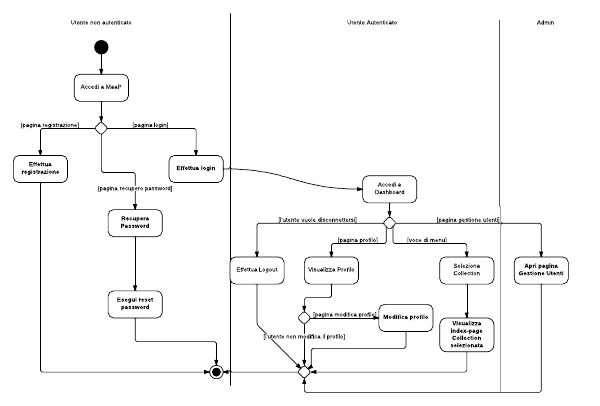
\includegraphics[scale=0.3]{uml/MaaP - Attivita principali.png}
\caption{Diagramma di attività - Attività principali di un'applicazione MaaP}
\end{figure}

Sostanzialmente un'applicazione generata da \glossario{MaaP} è composta da una serie di pagine web all'interno delle quali un utente può navigare. Un utente accede inizialmente all'applicazione web in una pagina statica in cui può effettuare tre cose:

\begin{itemize}

	\item Registrarsi al sistema;
	\item Effettuare il login;
	\item Recuperare la propria password.

\end{itemize}

Una volta che l'utente ha effettuato il login viene direttamente indirizzato alla \glossario{Dashboard}, dalla quale può navigare all'interno dell'applicazione ed effettuare diverse operazioni:

\begin{itemize}

	\item Effettuare il logout;
	\item Visualizzare il proprio profilo e di conseguenza modificarlo;
	\item Selezionare una \glossario{Collection} esistente.

\end{itemize}

Nel caso in cui l'utente avesse i privilegi di admin può inoltre accedere ad una specifica pagina di gestione degli utenti iscritti.

\subsubsection{Effettua registrazione}

\begin{figure}[H]
\centering
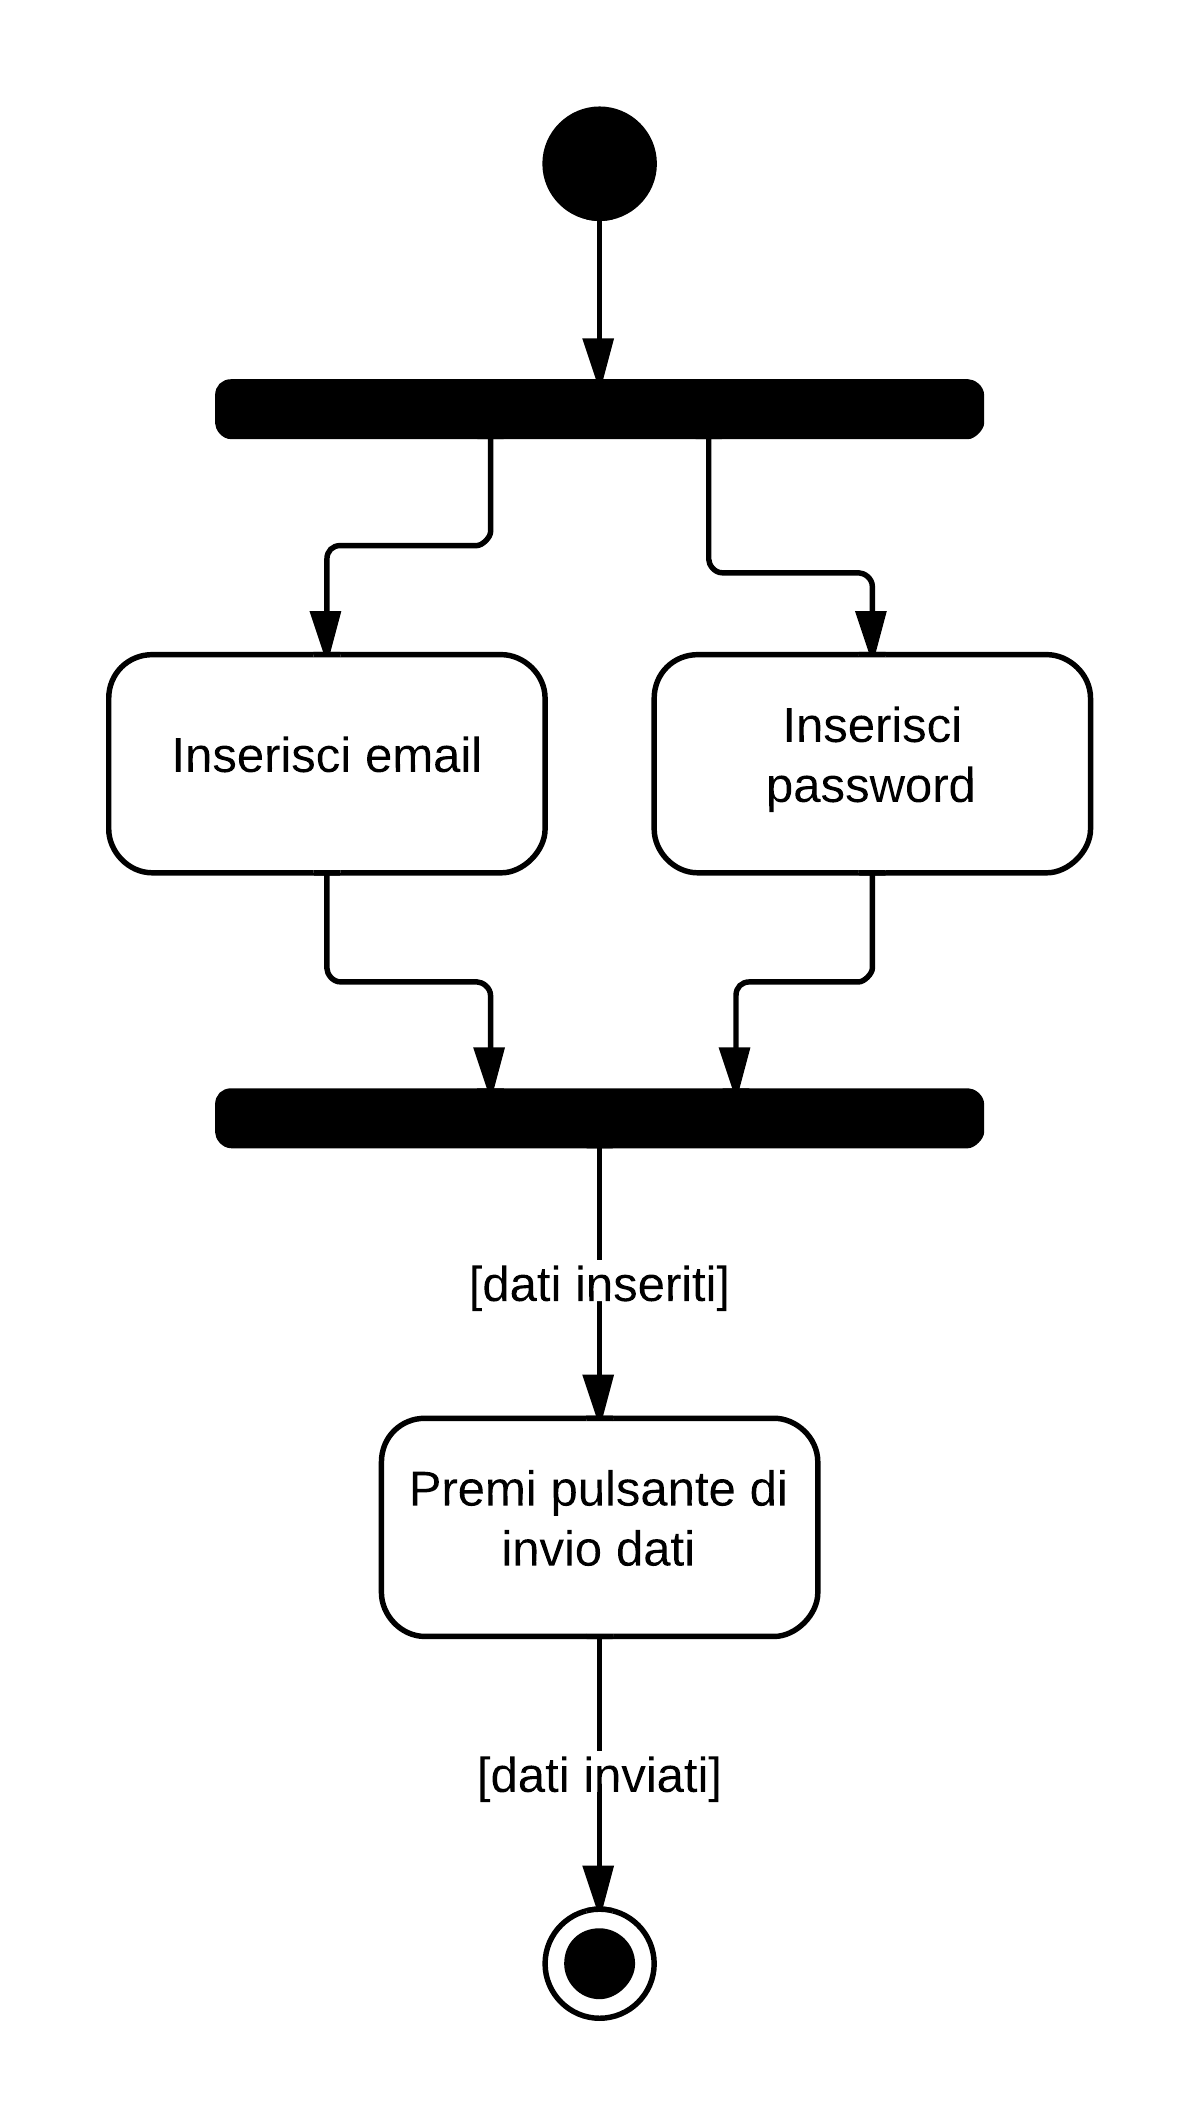
\includegraphics[scale=0.1]{uml/MaaP - Effettua registrazione.png}
\caption{Diagramma di attività - Registrazione di un utente}
\end{figure}

L'utente si trova all'interno della pagina di registrazione e sostanzialmente deve inserire la propria email e la propria password all'interno di due campi di testo. Una volta inseriti l'utente deve premere il pulsante di invio dati; il sistema \glossario{MaaP} procederà dunque alla verifica delle credenziali e, se quest'ultima avrà successo, alla registrazione dell'utente.

\subsubsection{Recupera password}

\begin{figure}[H]
\centering
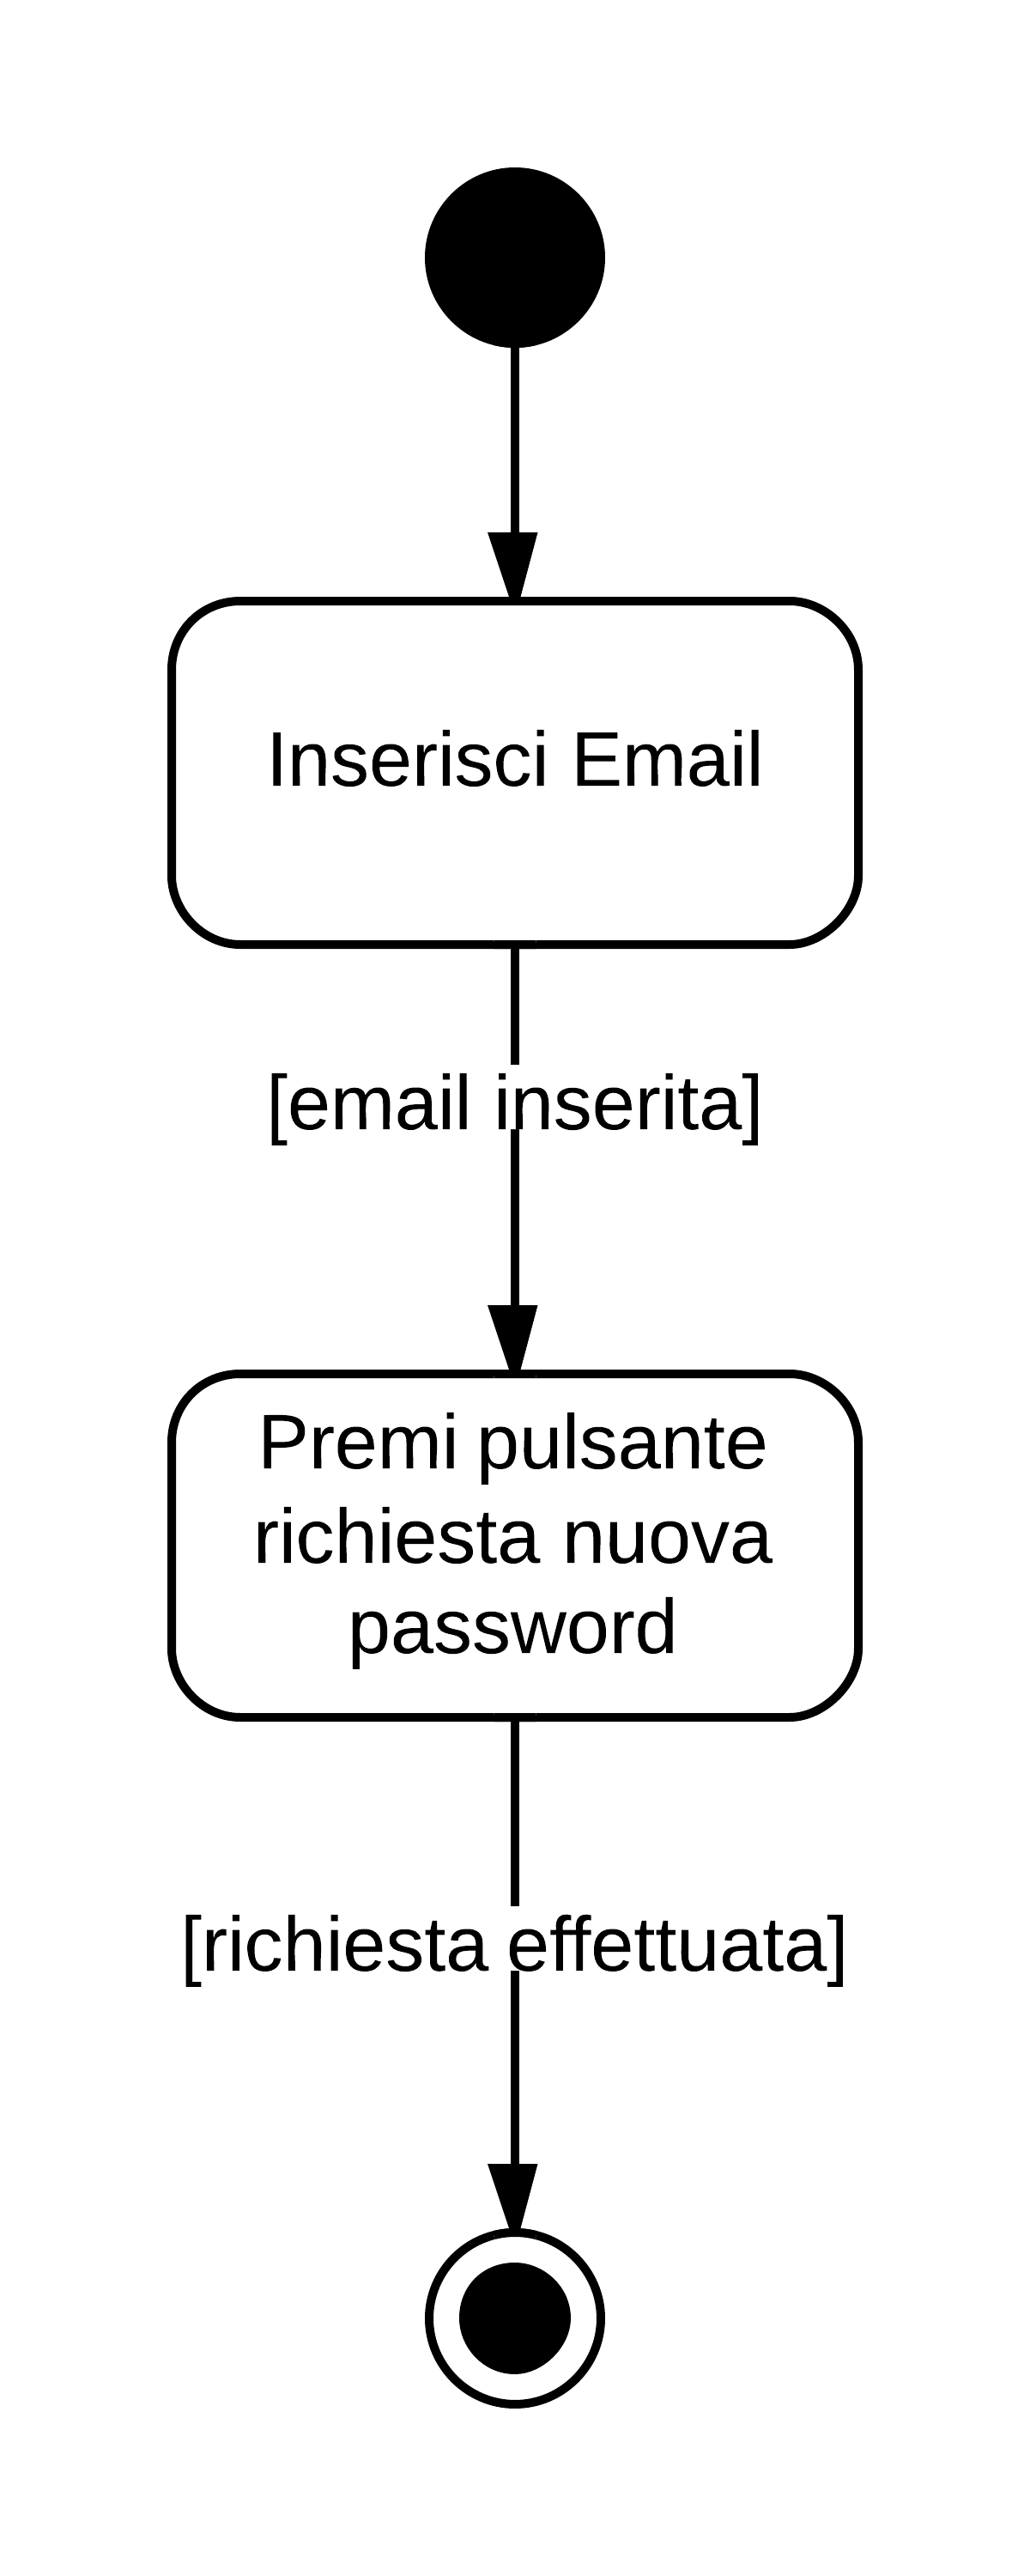
\includegraphics[scale=0.05]{uml/MaaP - Recupera password.png}
\caption{Diagramma di attività - Recupero password}
\end{figure}

L'utente si trova all'interno della pagina di recupero password, la quale presenta un campo di testo nel quale l'utente dovrà inserire il proprio indirizzo email. Una volta inserito preme il pulsante di richiesta di una nuova password; il sistema \glossario{MaaP} procederà dunque alla verifica dell'indirizzo email e, se quest'ultima avrà esito positivo, invierà un'email all'utente con le relative istruzioni per il ripristino della password.

\subsubsection{Esegui reset password}

\begin{figure}[H]
\centering
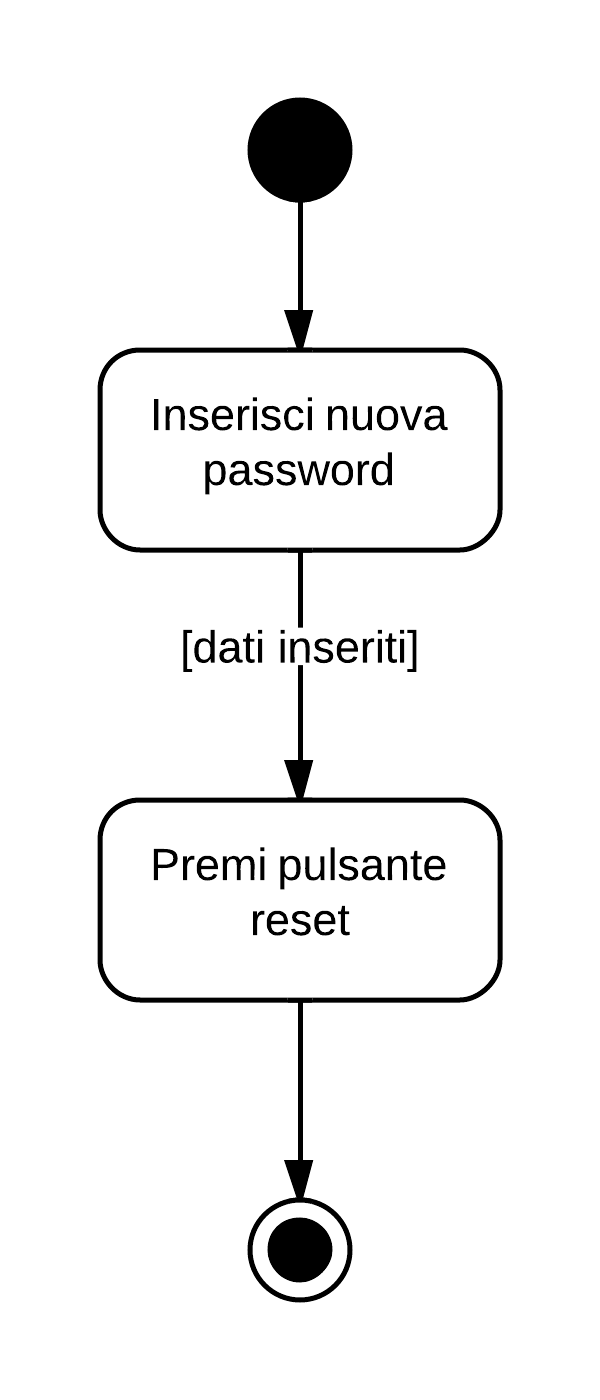
\includegraphics[scale=0.05]{uml/MaaP - Esegui reset password.png}
\caption{Diagramma di attività - Reset della password dell'utente}
\end{figure}

L'utente avrà ricevuto un'email con al suo interno un link ad una pagina univoca dell'applicazione \glossario{MaaP} e quindi si troverà in una pagina con al suo interno un campo di testo nel quale inserire la nuova password. Una volta inserita la password deve premere il pulsante di reset; il sistema \glossario{MaaP} procederà dunque al cambio password per l'utente corrente nel \glossario{database} delle credenziali.

\subsubsection{Effettua login}

\begin{figure}[H]
\centering
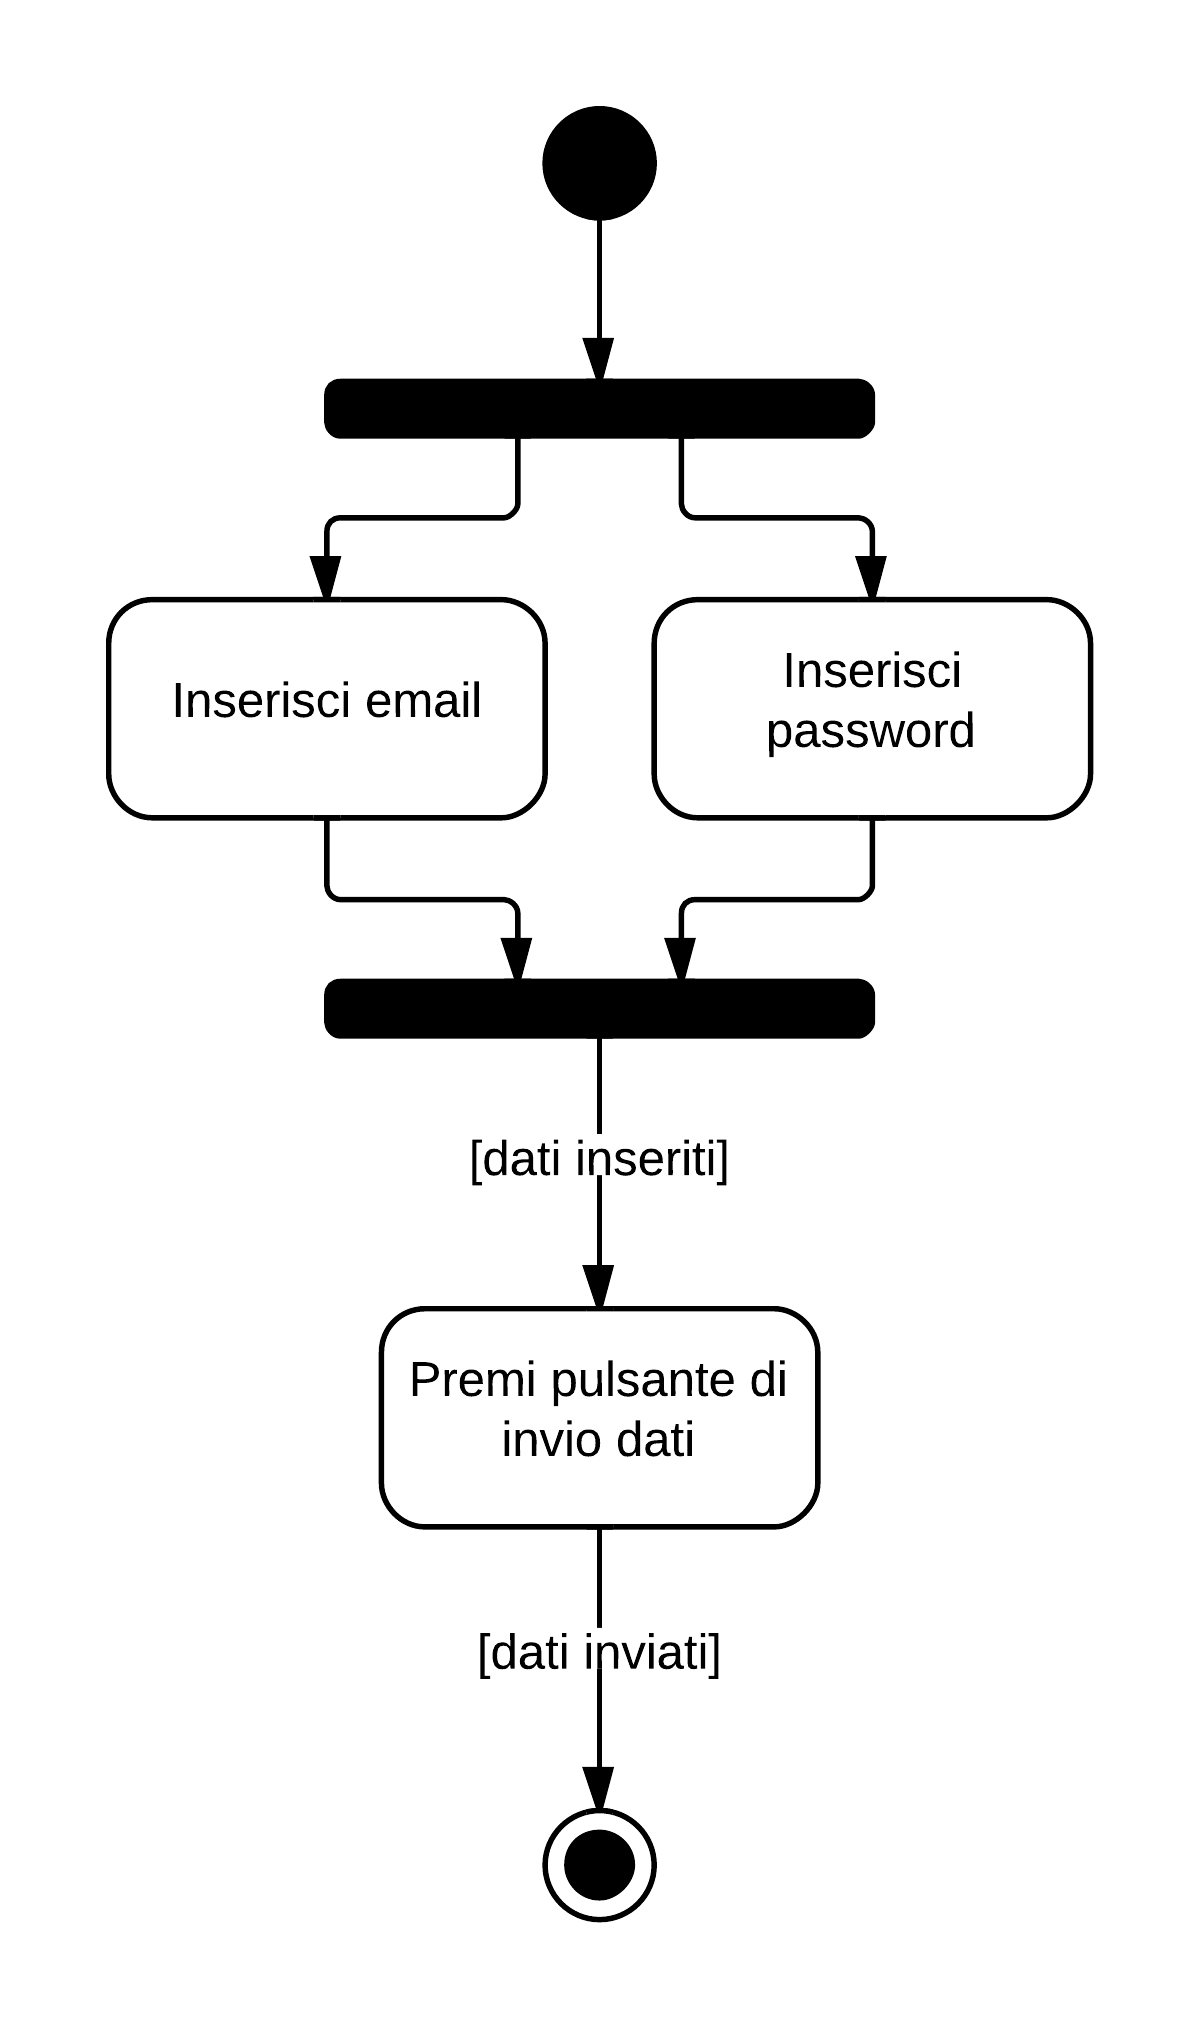
\includegraphics[scale=0.1]{uml/MaaP - Effettua login.png}
\caption{Diagramma di attività - Login dell'utente}
\end{figure}

L'utente, che precedentemente avrà effettuato la registrazione al sistema, accede all'interno dell'applicazione tramite una pagina di login. Al suo interno saranno presenti due campi di testo in cui l'utente dovrà inserire la propria email e la propria password. Una volta inserite dovrà premere il pulsante di login; il sistema \glossario{MaaP} procederà dunque alla verifica delle credenziali e, se l'esito di tale verifica risulterà positivo, effettuerà il login dell'utente all'applicazione, reindirizzandolo alla \glossario{dashboard}.

\subsubsection{Modifica profilo}

\begin{figure}[H]
\centering
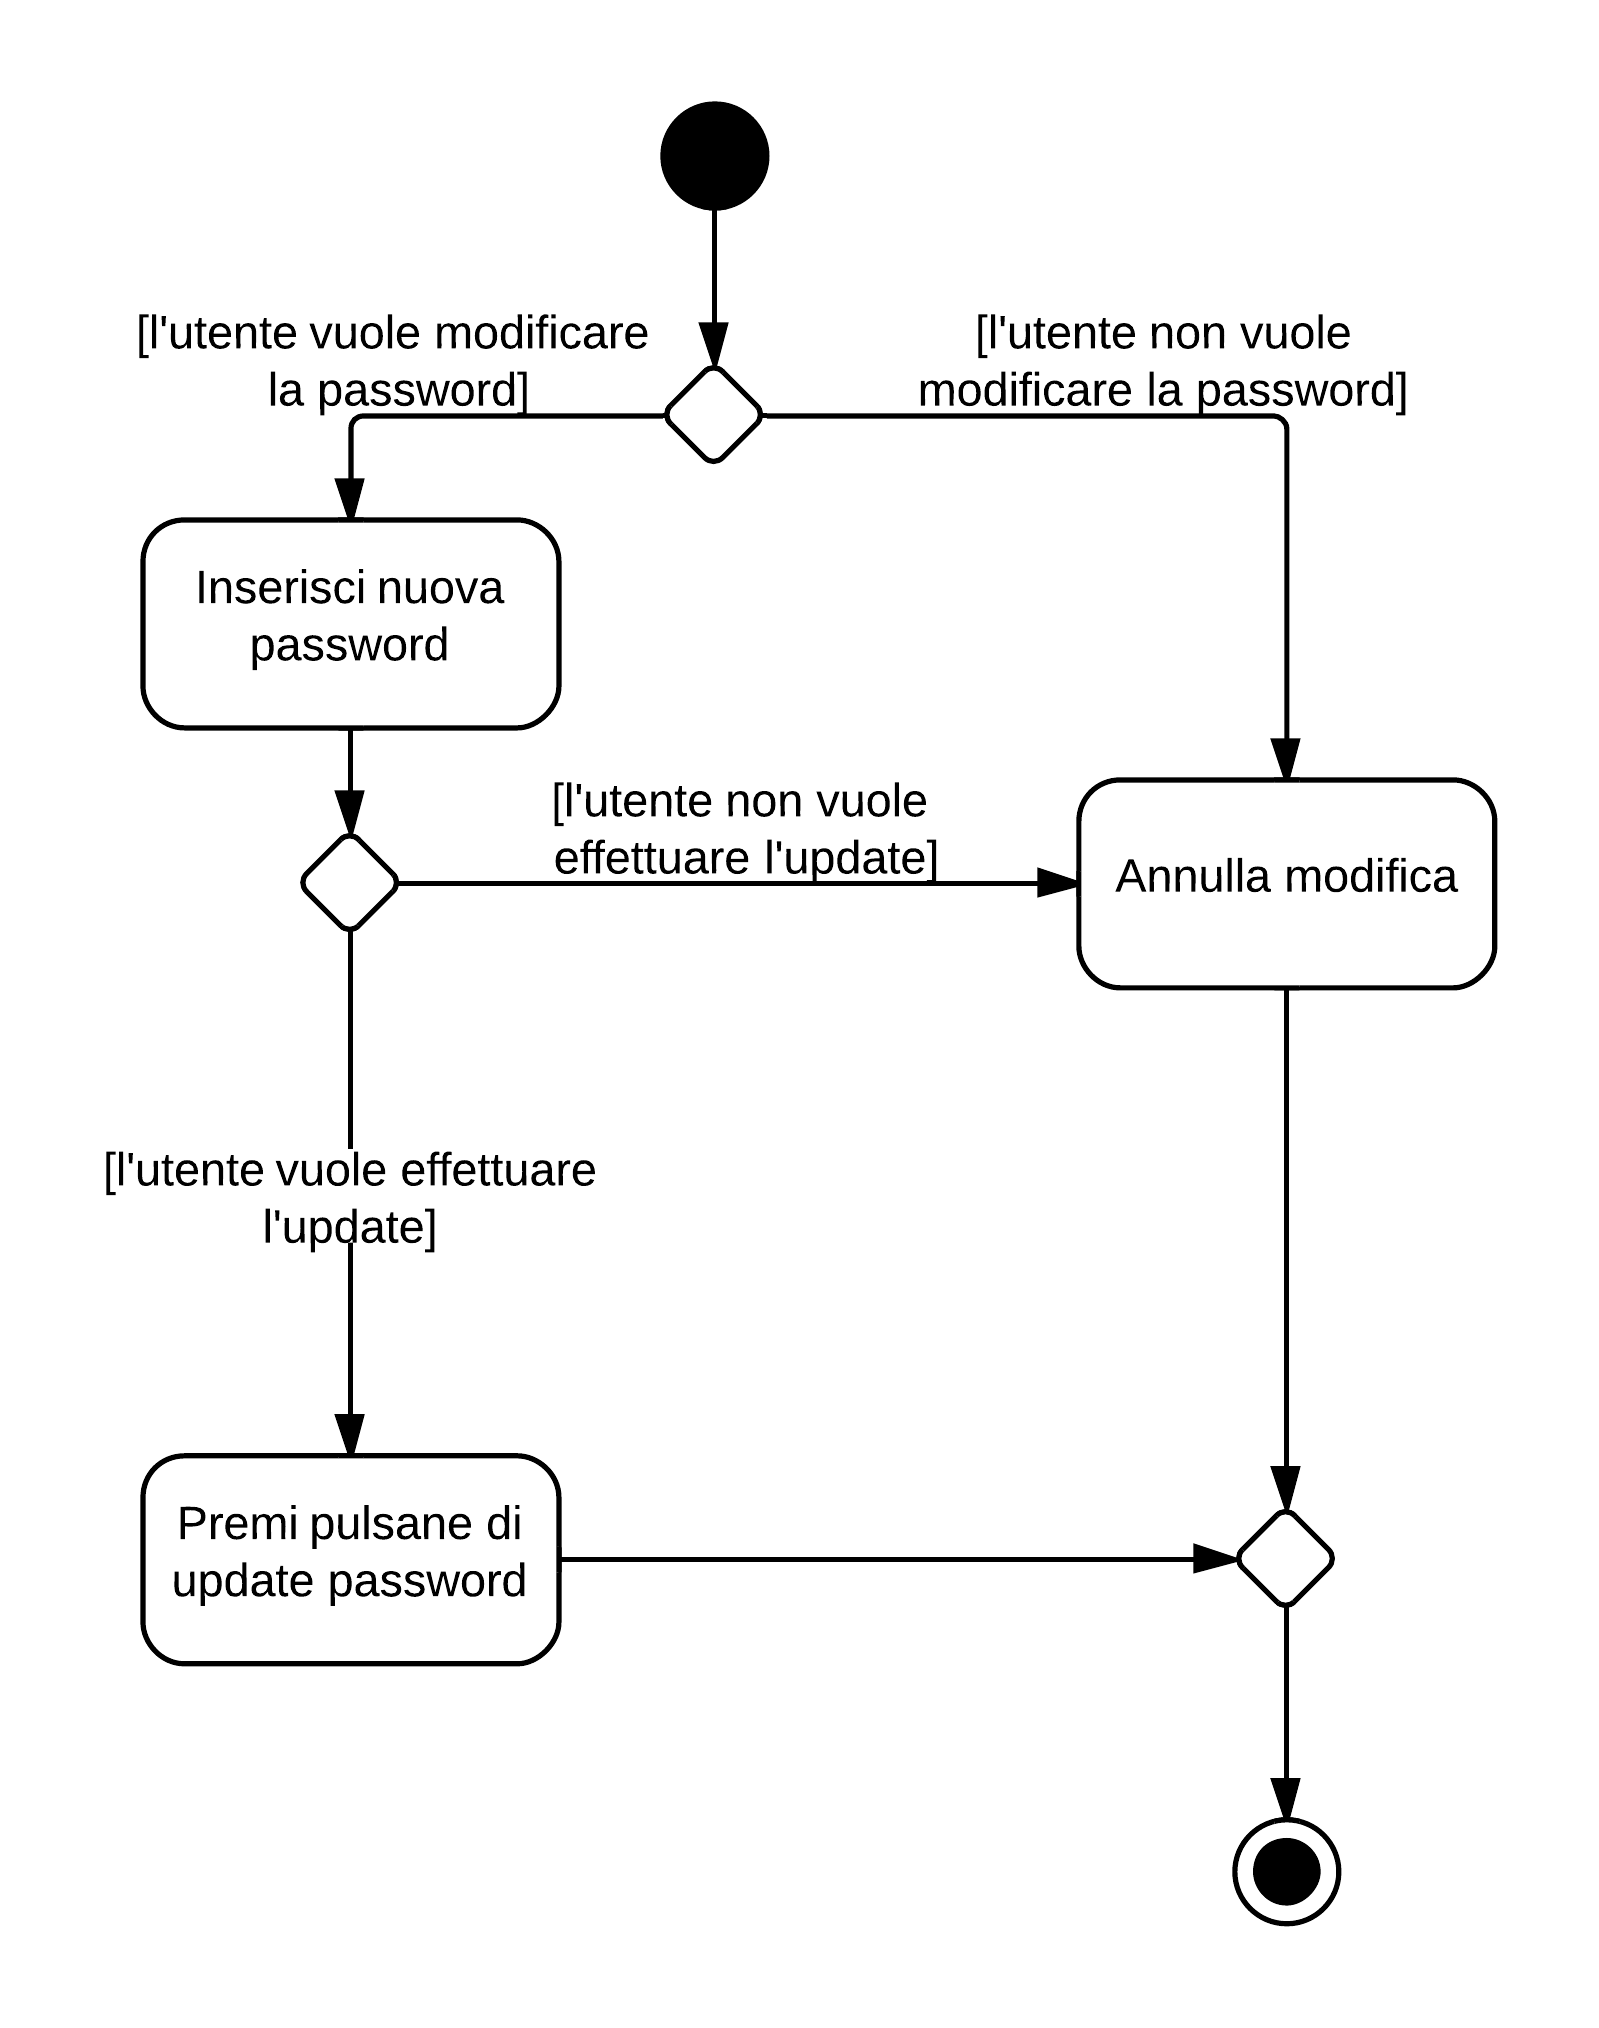
\includegraphics[scale=0.1]{uml/MaaP - Modifica profilo.png}
\caption{Diagramma di attività - Modifica profilo utente}
\end{figure}

L'utente autenticato accede all'interno della propria pagina profilo, dalla quale può decidere di modificare la propria password. Sarà dunque presente un campo di testo in cui l'utente inserirà la nuova password e un bottone tramite il quale invierà la richiesta di modifica; il sistema \glossario{MaaP} procederà dunque alla modifica della password dell'utente. L'utente in ogni momento può decidere di annullare le modifiche e tornare alla pagina precedente.

\subsubsection{Index-page Collection}

\begin{figure}[H]
\centering
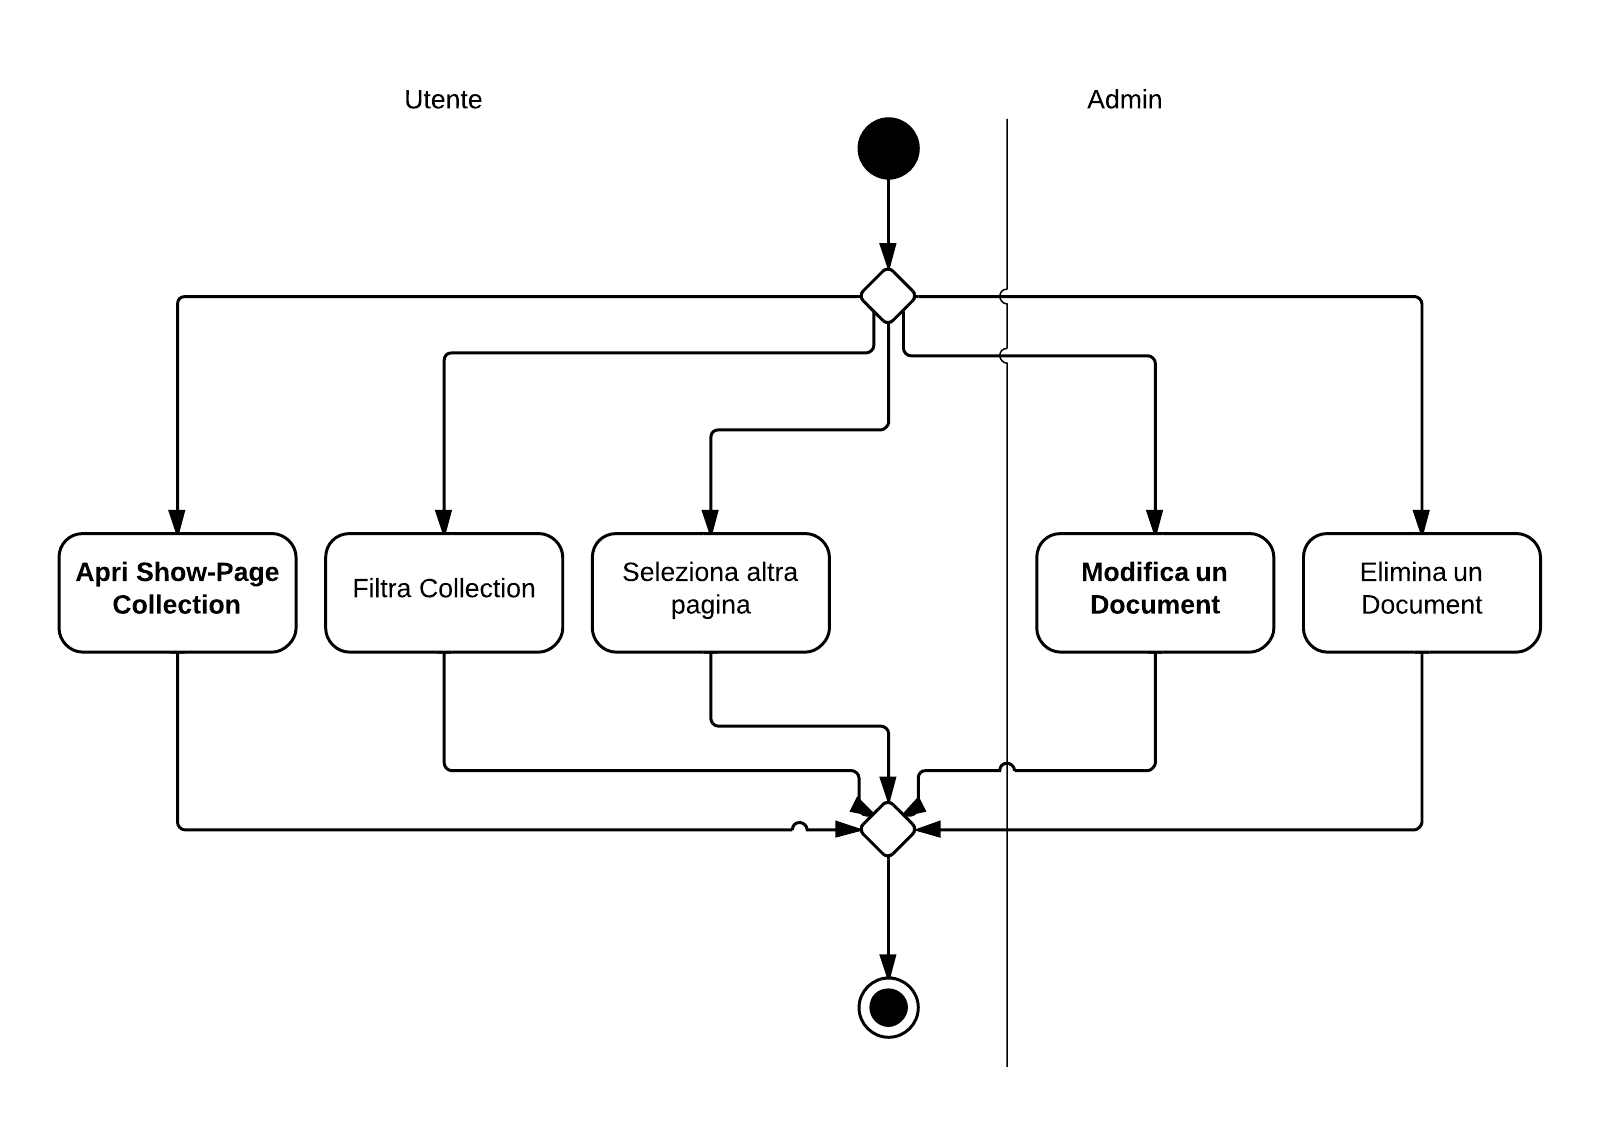
\includegraphics[scale=0.2]{uml/MaaP - Index-page.png}
\caption{Diagramma di attività - Visualizzazione index-page della Collection selezionata}
\end{figure}

L'utente ha selezionato una \glossario{Collection} dal menu e ora si trova all'interno di una pagina che visualizza una tabella contenente tutti i \glossario{Document} della \glossario{Collection} con alcuni attributi visualizzabili. A questo punto è in grado di fare diverse operazioni:

\begin{itemize}

	\item Può aprire la relativa \glossario{show-page} di un \glossario{Document} selezionando il link che la apre;
	\item Può applicare un filtro ai \glossario{Document} visualizzati in modo da visualizzare un sottoinsieme della tabella;
	\item Se la tabella risulta distribuita su più pagine può accedere alle pagine successive;

\end{itemize}

Se l'utente dispone dei privilegi di admin può inoltre:

\begin{itemize}

	\item Modificare un \glossario{Document} cliccando sul link \textit{edit} visualizzato in ciascuna riga della tabella;
	\item Eliminare un \glossario{Document} cliccando sul link \textit{delete} visualizzato in ciascuna riga della tabella;

\end{itemize}

\subsubsection{Show-page Document}

\begin{figure}[H]
\centering
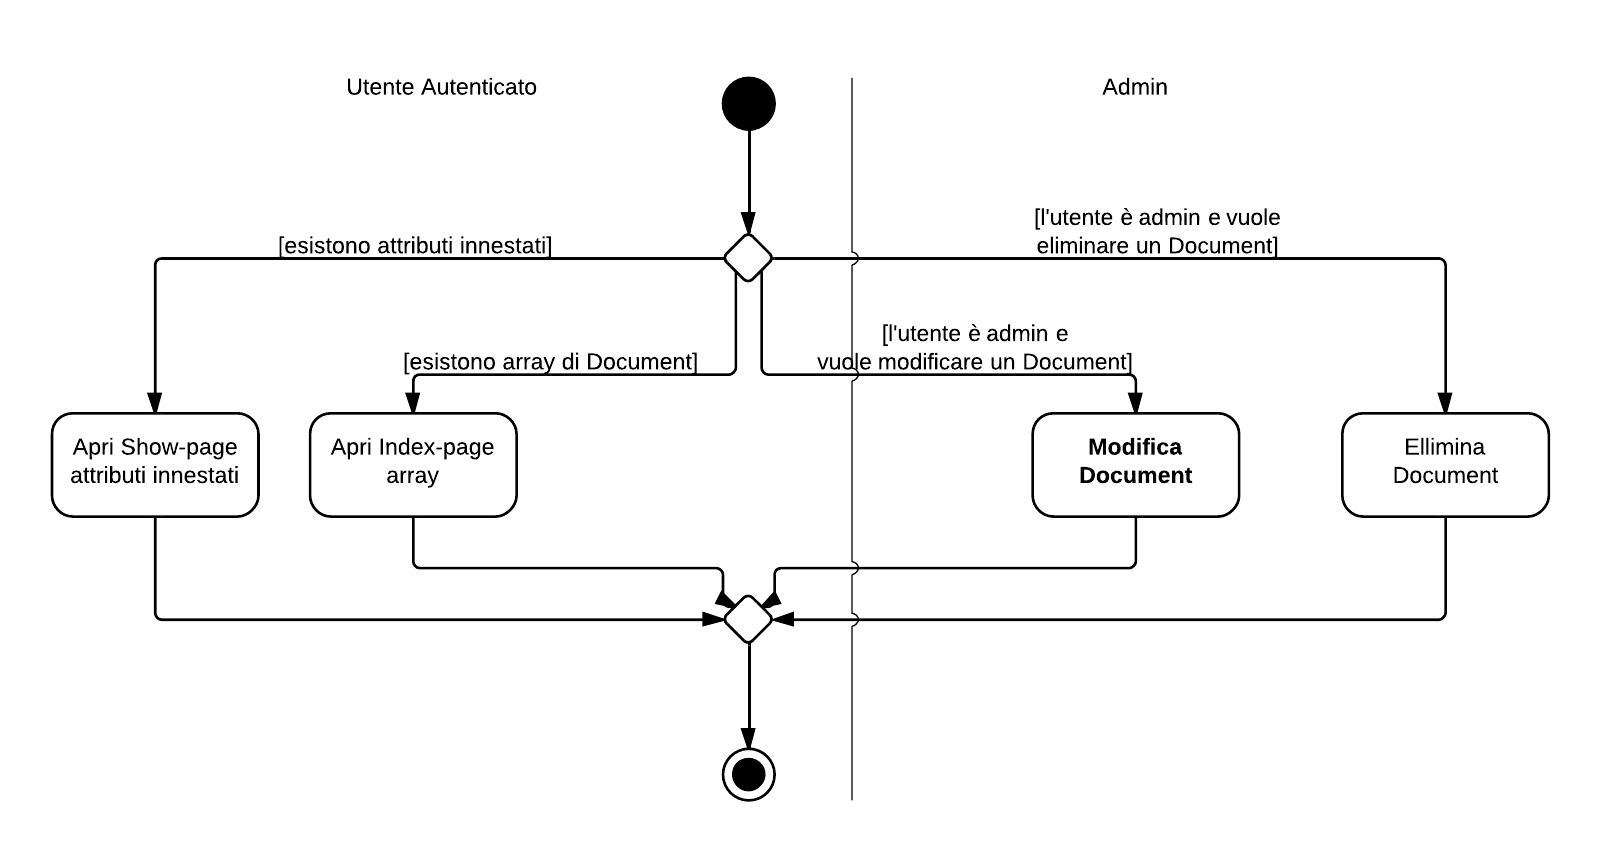
\includegraphics[scale=0.2]{uml/MaaP - Show-page.png}
\caption{Diagramma di attività - Visualizzazione show-page del Document selezionato}
\end{figure}

L'utente ha selezionato un \glossario{Document} dalla \glossario{index-page} e ora si trova davanti una pagina di visualizzazione dettagliata del \glossario{Document} selezionato. Sostanzialmente questa pagina conterrà una tabella contenente gli attributi visualizzabili del \glossario{Document}. Un utente all'interno di questa pagina può:

\begin{itemize}

	\item Aprire la \glossario{show-page} di un attributo innestato, se ne esiste uno;
	\item Aprire la \glossario{index-page} di un array di \glossario{Document}, se ne esiste uno.

\end{itemize}

Se l'utente possiede i privilegi di admin può inoltre:

\begin{itemize}

	\item Modificare gli attributi del \glossario{Document};
	\item Eliminare il \glossario{Document} corrente.

\end{itemize}

\subsubsection{Modifica Document}

\begin{figure}[H]
\centering
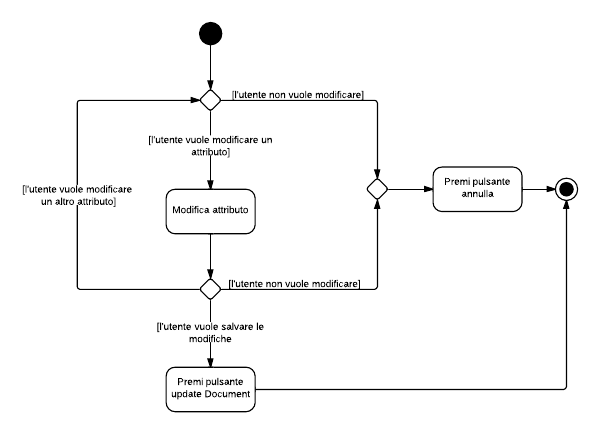
\includegraphics[scale=0.2]{uml/MaaP - Modifica document.png}
\caption{Diagramma di attività - Modifica del Document selezionato}
\end{figure}

L'utente con privilegi di scrittura può modificare ogni singolo attributo del \glossario{Document} selezionato, editando i rispettivi campi di testo. Una volta che ha terminato le modifiche preme il pulsante di \textit{update}; il sistema \glossario{MaaP} verificherà che le modifiche apportate siano corrette e rispettino i vincoli del \glossario{database}. In ogni momento l'utente può comunque decidere di annullare le modifiche e tornare alla pagina precedente.

\subsubsection{Apri pagina gestione utenti}

\begin{figure}[H]
\centering
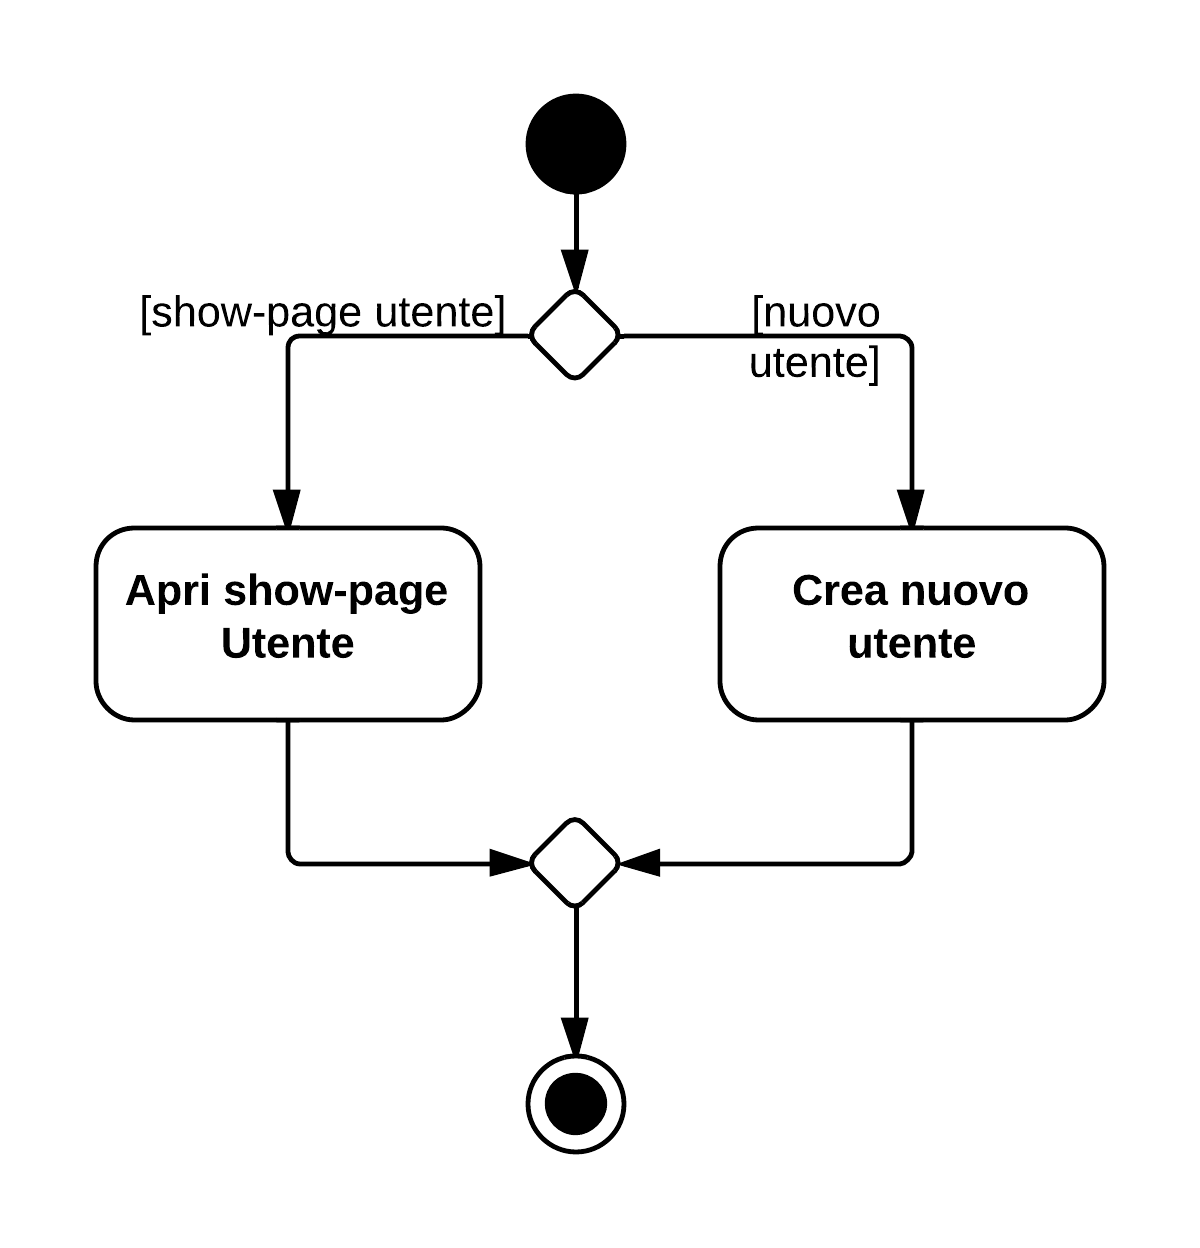
\includegraphics[scale=0.1]{uml/MaaP - Apri pagina gestione utenti.png}
\caption{Diagramma di attività - Pagina di gestione degli utenti}
\end{figure}

Un admin dell'applicazione può accedere a una pagina in cui poter gestire gli utenti. Essa consiste fondamentalmente in una \glossario{index-page} contenente la lista di tutti gli utenti presenti nel sistema. L'admin può da questa pagina selezionare un utente, e visualizzare quindi la sua relativa \glossario{show-page}, o crearne uno nuovo aprendo la pagina di creazione.

\subsubsection{Apri show-page utente}

\begin{figure}[H]
\centering
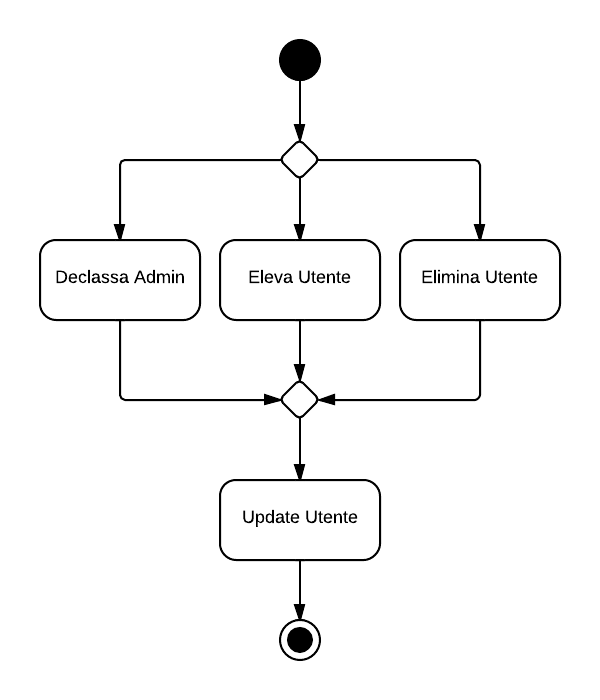
\includegraphics[scale=0.2]{uml/MaaP - Apri show-page utente.png}
\caption{Diagramma di attività - Pagina di visualizzazione di un utente}
\end{figure}

In questa pagina l'admin visualizza la \glossario{show-page} dell'utente selezionato e può compiere le seguenti operazioni:

\begin{itemize}

	\item Se l'utente selezionato è un admin può declassarlo e portarlo a livello di utente normale. Naturalmente non può declassare se stesso e il \textit{super-admin}, in modo da far sì che in qualsiasi momento sia presente almeno un admin nel sistema;
	\item Se l'utente non è un admin può elevarlo da utente normale a livello di admin;
	\item Eliminare l'utente selezionato dal sistema.

\end{itemize}

Il sistema \glossario{MaaP} si occuperò di apportare tutte le modifiche effettuate dall'admin al \glossario{database} delle credenziali.

\subsubsection{Crea un nuovo utente}

\begin{figure}[H]
\centering
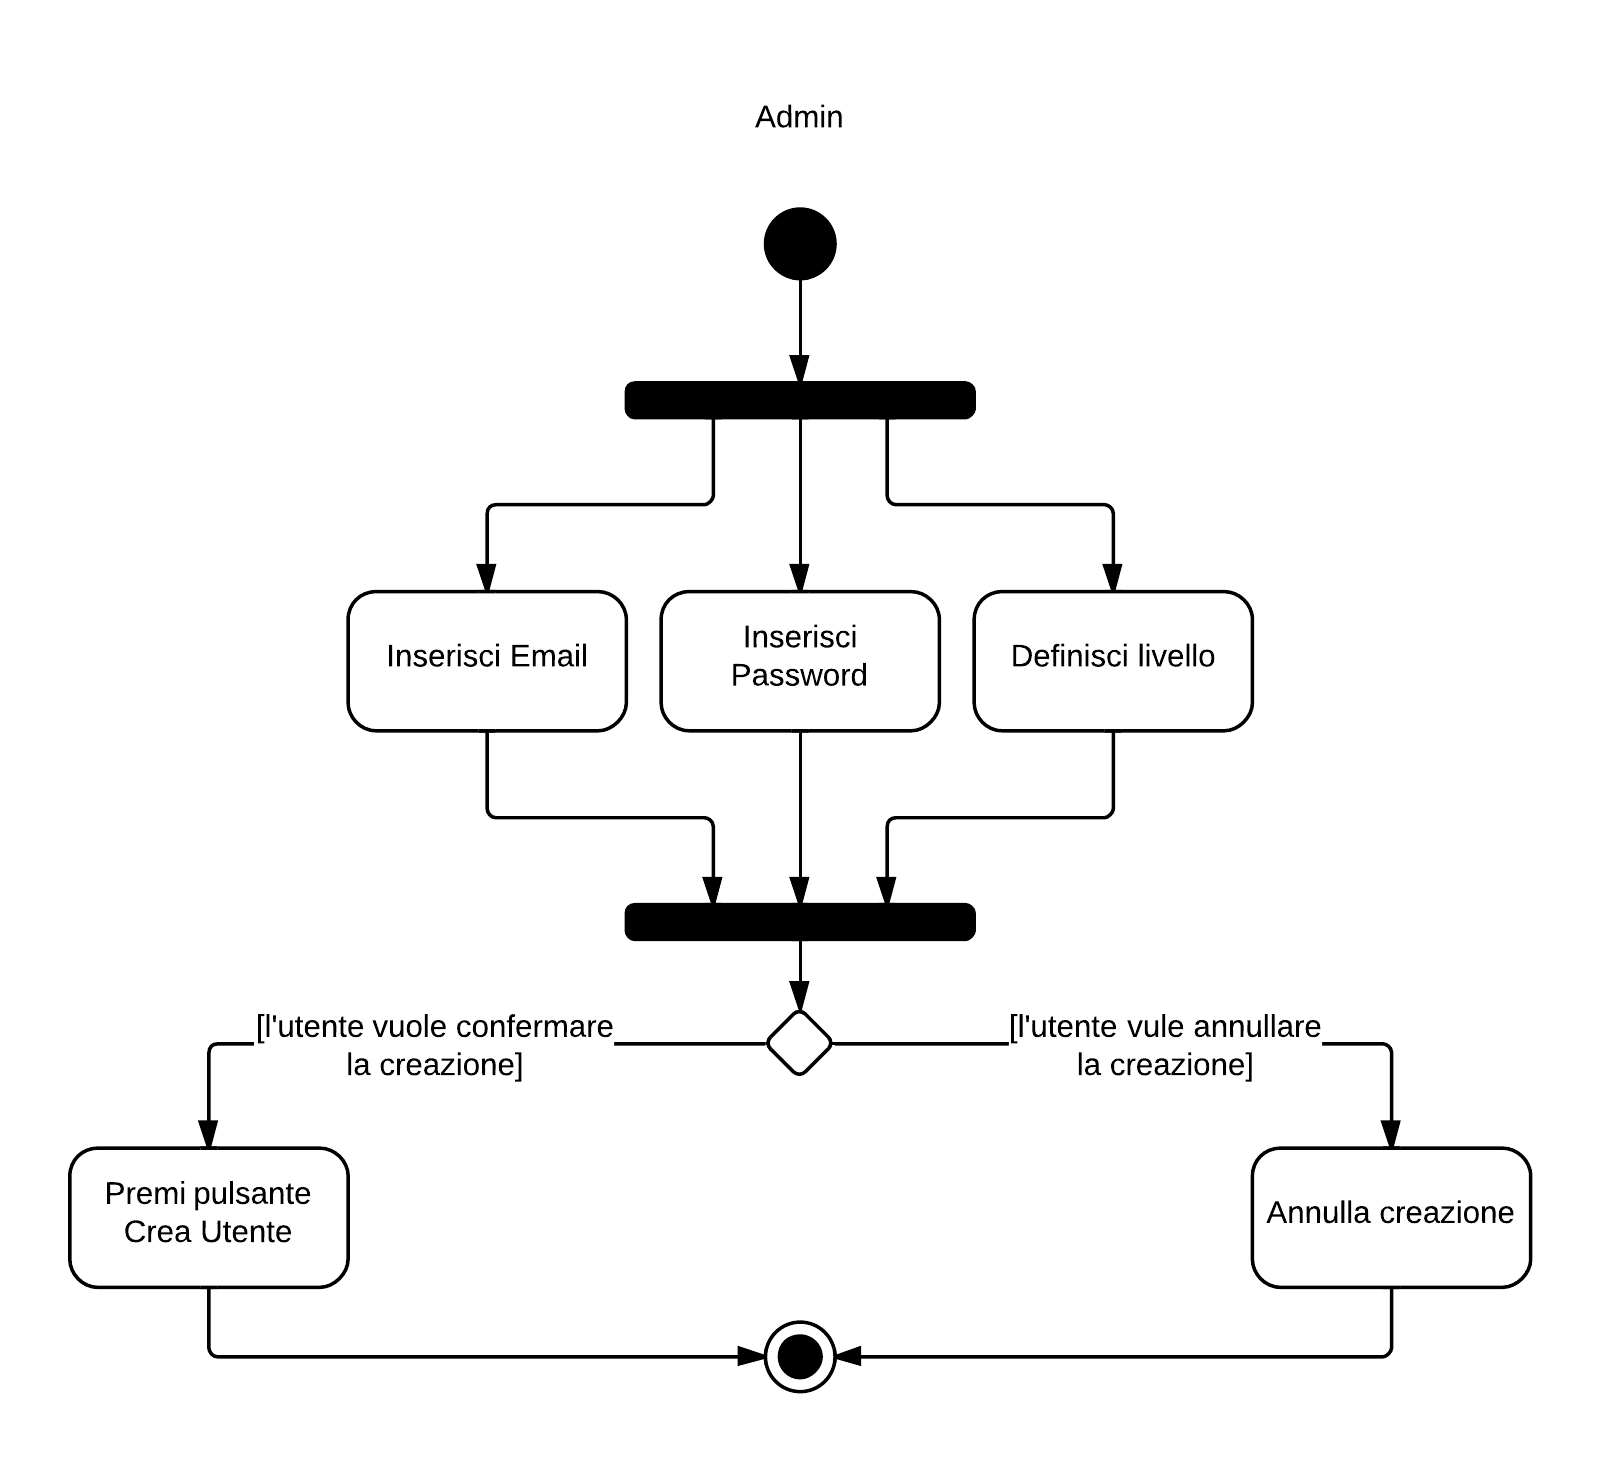
\includegraphics[scale=0.2]{uml/MaaP - Crea nuovo utente.png}
\caption{Diagramma di attività - Pagina di creazione di un nuovo utente}
\end{figure}

L'admin entra in un'apposita pagina di creazione di un nuovo utente e al suo interno può definire:

\begin{itemize}

	\item L'indirizzo email del nuovo utente;
	\item La password del nuovo utente;
	\item Il livello del nuovo utente, che potrà essere o utente normale o admin;

\end{itemize}

Una volta completate le modifiche l'utente può decidere di confermare o annullare le modifiche, premendo i relativi pulsanti. Il sistema \glossario{MaaP}, nel caso in cui l'utente abbia deciso di confermare le modifiche, si occuperà di inserire nel \glossario{database} delle credenziali il nuovo utente creato.

%\subsection{Servizio MaaS}
%
%Vengono di seguito descritte tutte le iterazioni che un utente può effettuare con il servizio web \glossario{MaaS}.
%
%\subsubsection{Attività principali}
%
%\begin{figure}[H]
%\centering
%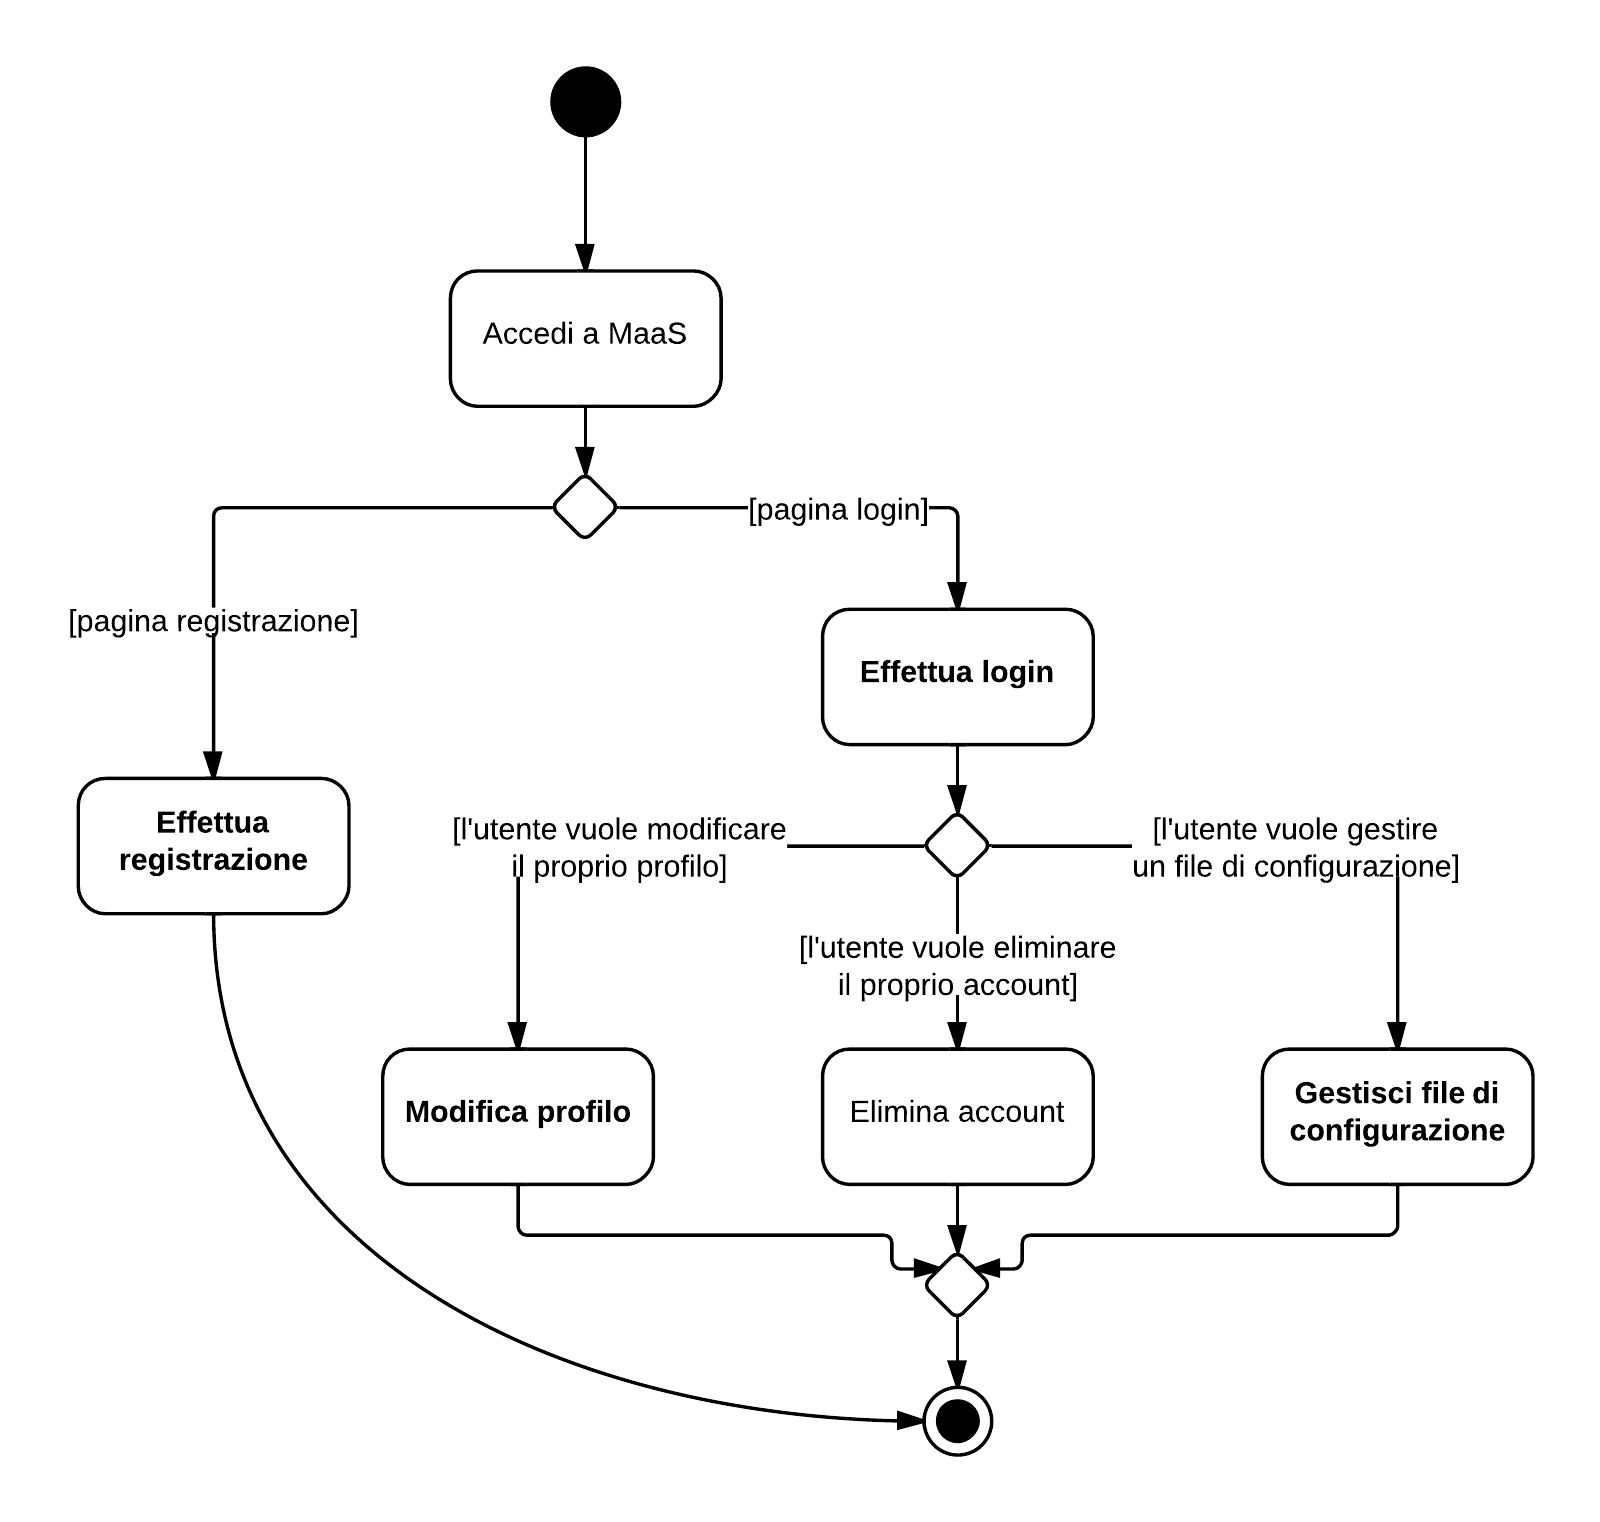
\includegraphics[scale=0.2]{uml/MaaS - Attivita principali.png}
%\caption{Diagramma di attività - Attività principali di MaaS}
%\end{figure}
%
%L'utente sviluppatore accede tramite il proprio browser al servizio \glossario{MaaS}, il quale gli richiederà l'autenticazione o gli offrirà la possibilità di registrarsi presso di esso. Una volta effettuato l'accesso l'utente si trova di fronte alla propria pagina personale, dalla quale può navigare su altre pagine. Può sostanzialmente effettuare le seguenti operazioni:
%
%\begin{itemize}
%
%	\item Modificare il proprio profilo, cambiando la password di accesso;
%	\item Eliminare il proprio account, eliminando di conseguenza tutti i file di configurazione ad esso associati;
%	\item Gestire i propri file di configurazione della propria applicazione.
%
%\end{itemize}
%
%\subsubsection{Effettua registrazione}
%
%\begin{figure}[H]
%\centering
%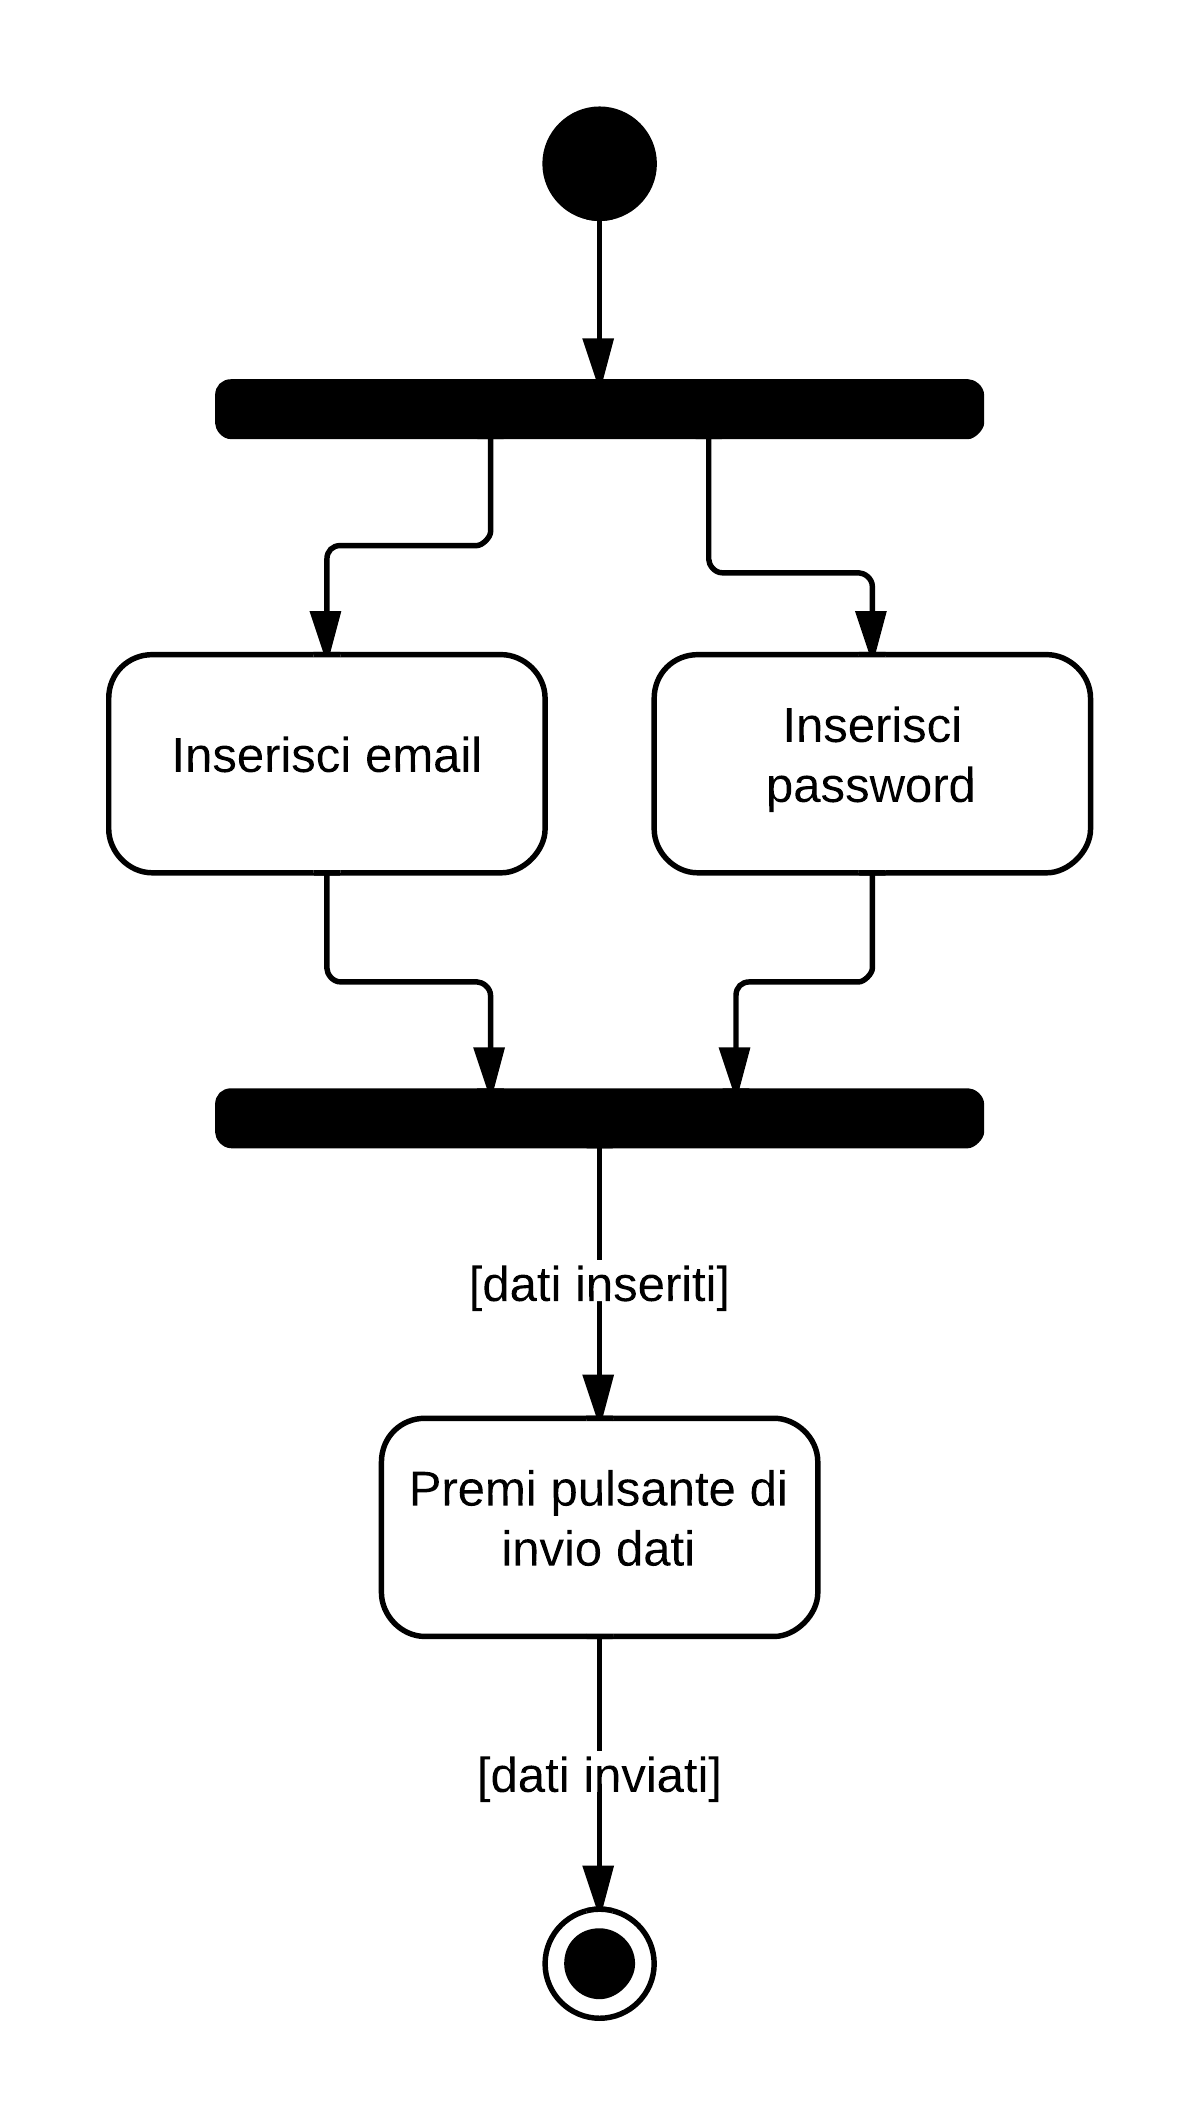
\includegraphics[scale=0.1]{uml/MaaP - Effettua registrazione.png}
%\caption{Diagramma di attività - Registrazione al servizio MaaS}
%\end{figure}
%
%In maniera pressoché identica da quanto offerto da un'applicazione \glossario{MaaP} l'utente visualizza una pagina di registrazione nella quale deve inserire in appositi campi di testo l'email e la password con le quali vuole registrarsi al servizio. Una volta inseriti i dati premerà il pulsante di richiesta registrazione. Il sistema procederà dunque alla verifica delle credenziali inserite e, se l'indirizzo email non è già presente, procederà alla registrazione del nuovo utente.
%
%\subsubsection{Effettua login}
%
%\begin{figure}[H]
%\centering
%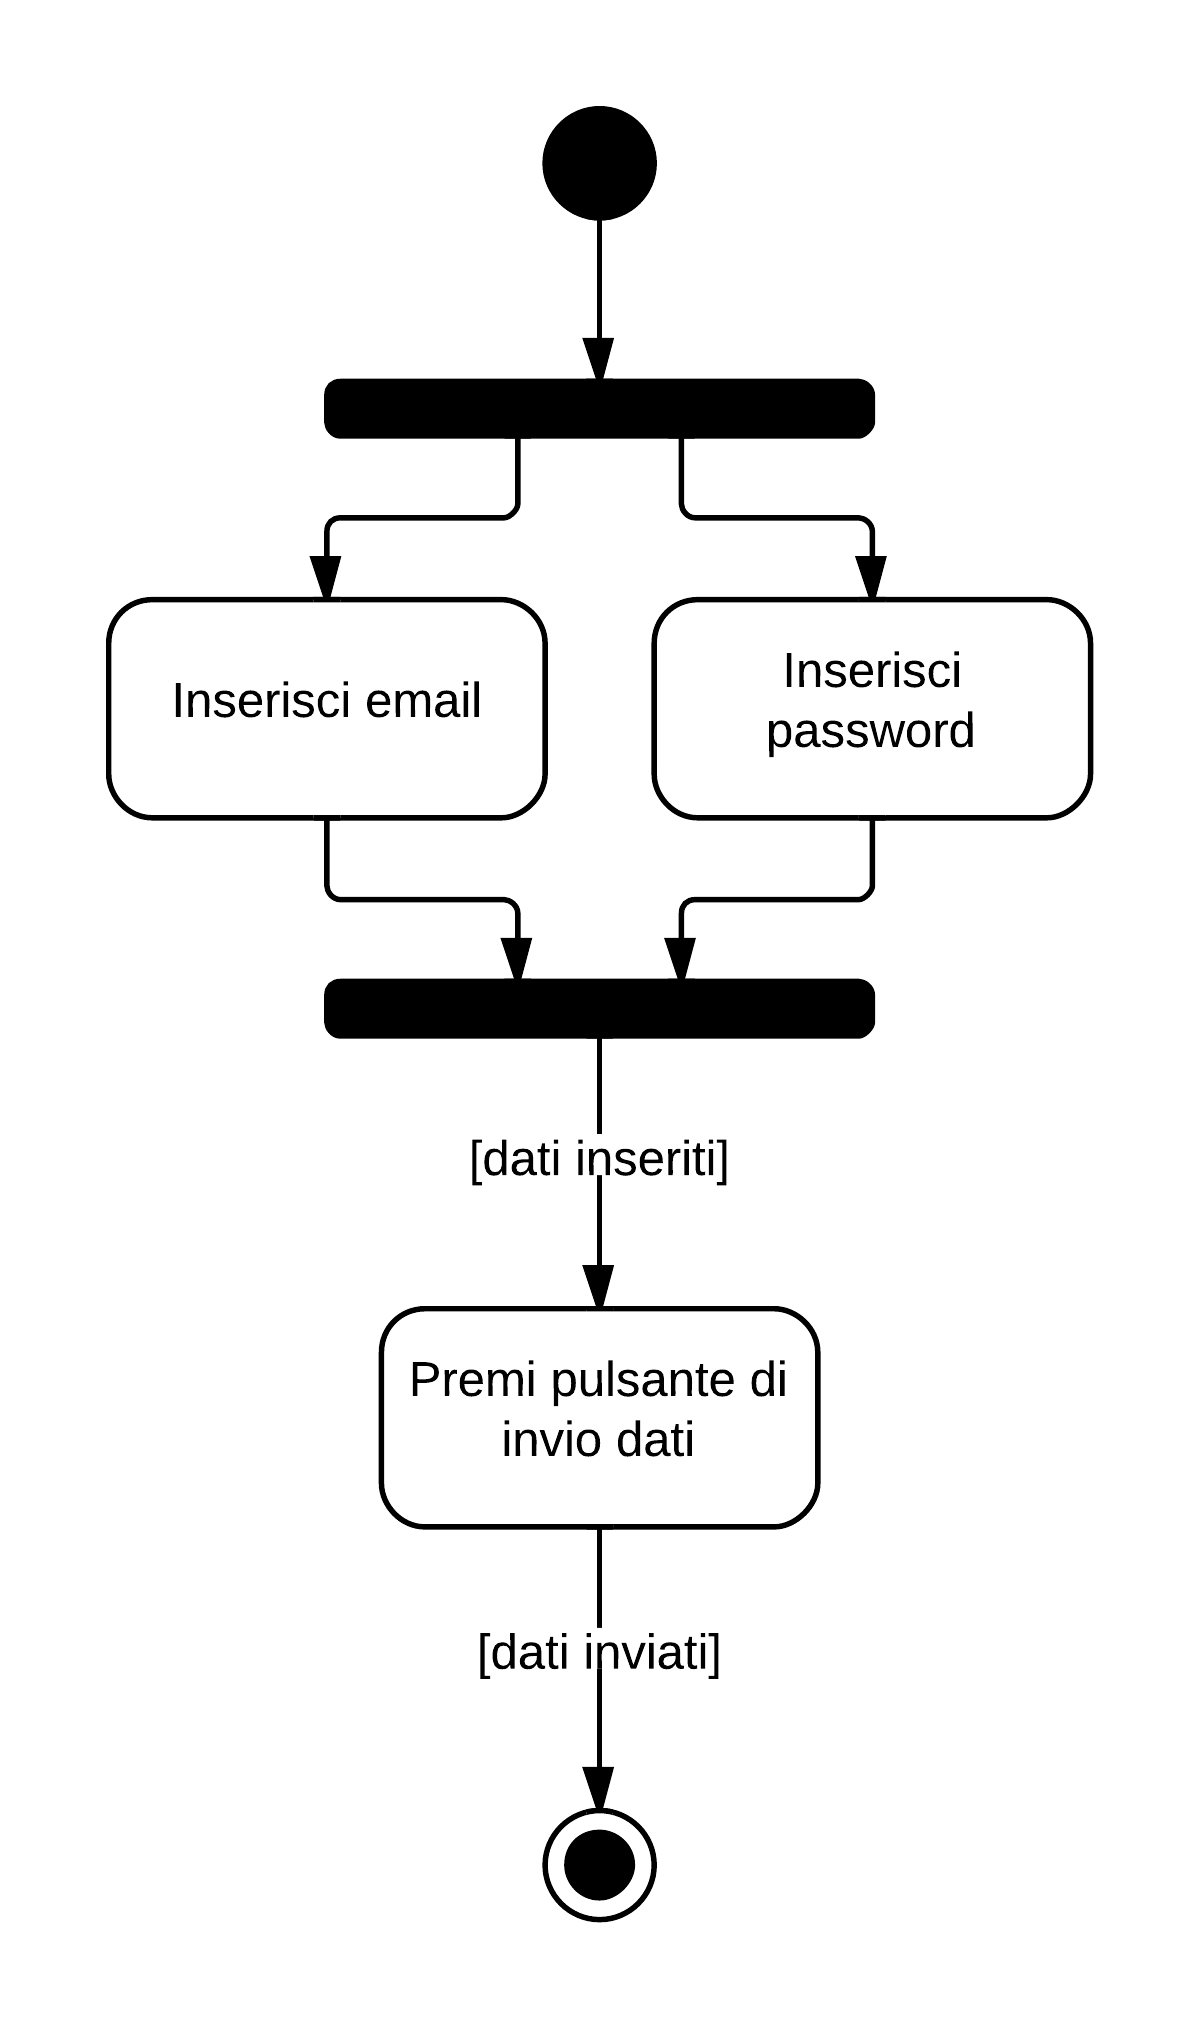
\includegraphics[scale=0.1]{uml/MaaP - Effettua login.png}
%\caption{Diagramma di attività - Login al servizio MaaS}
%\end{figure}
%
%In maniera pressoché identica da quanto offerto da un'applicazione \glossario{MaaP} l'utente visualizza una pagina di login nella quale deve inserire la propria email e la propria password in appositi campi di testo. Una volta inseriti i dati premerà quindi un pulsante per accedere al servizio \glossario{MaaS}. Il sistema si occuperà di verificare la correttezza delle credenziali e, in caso positivo, effettuerà il login dell'utente.
%
%\subsubsection{Modifica profilo}
%
%\begin{figure}[H]
%\centering
%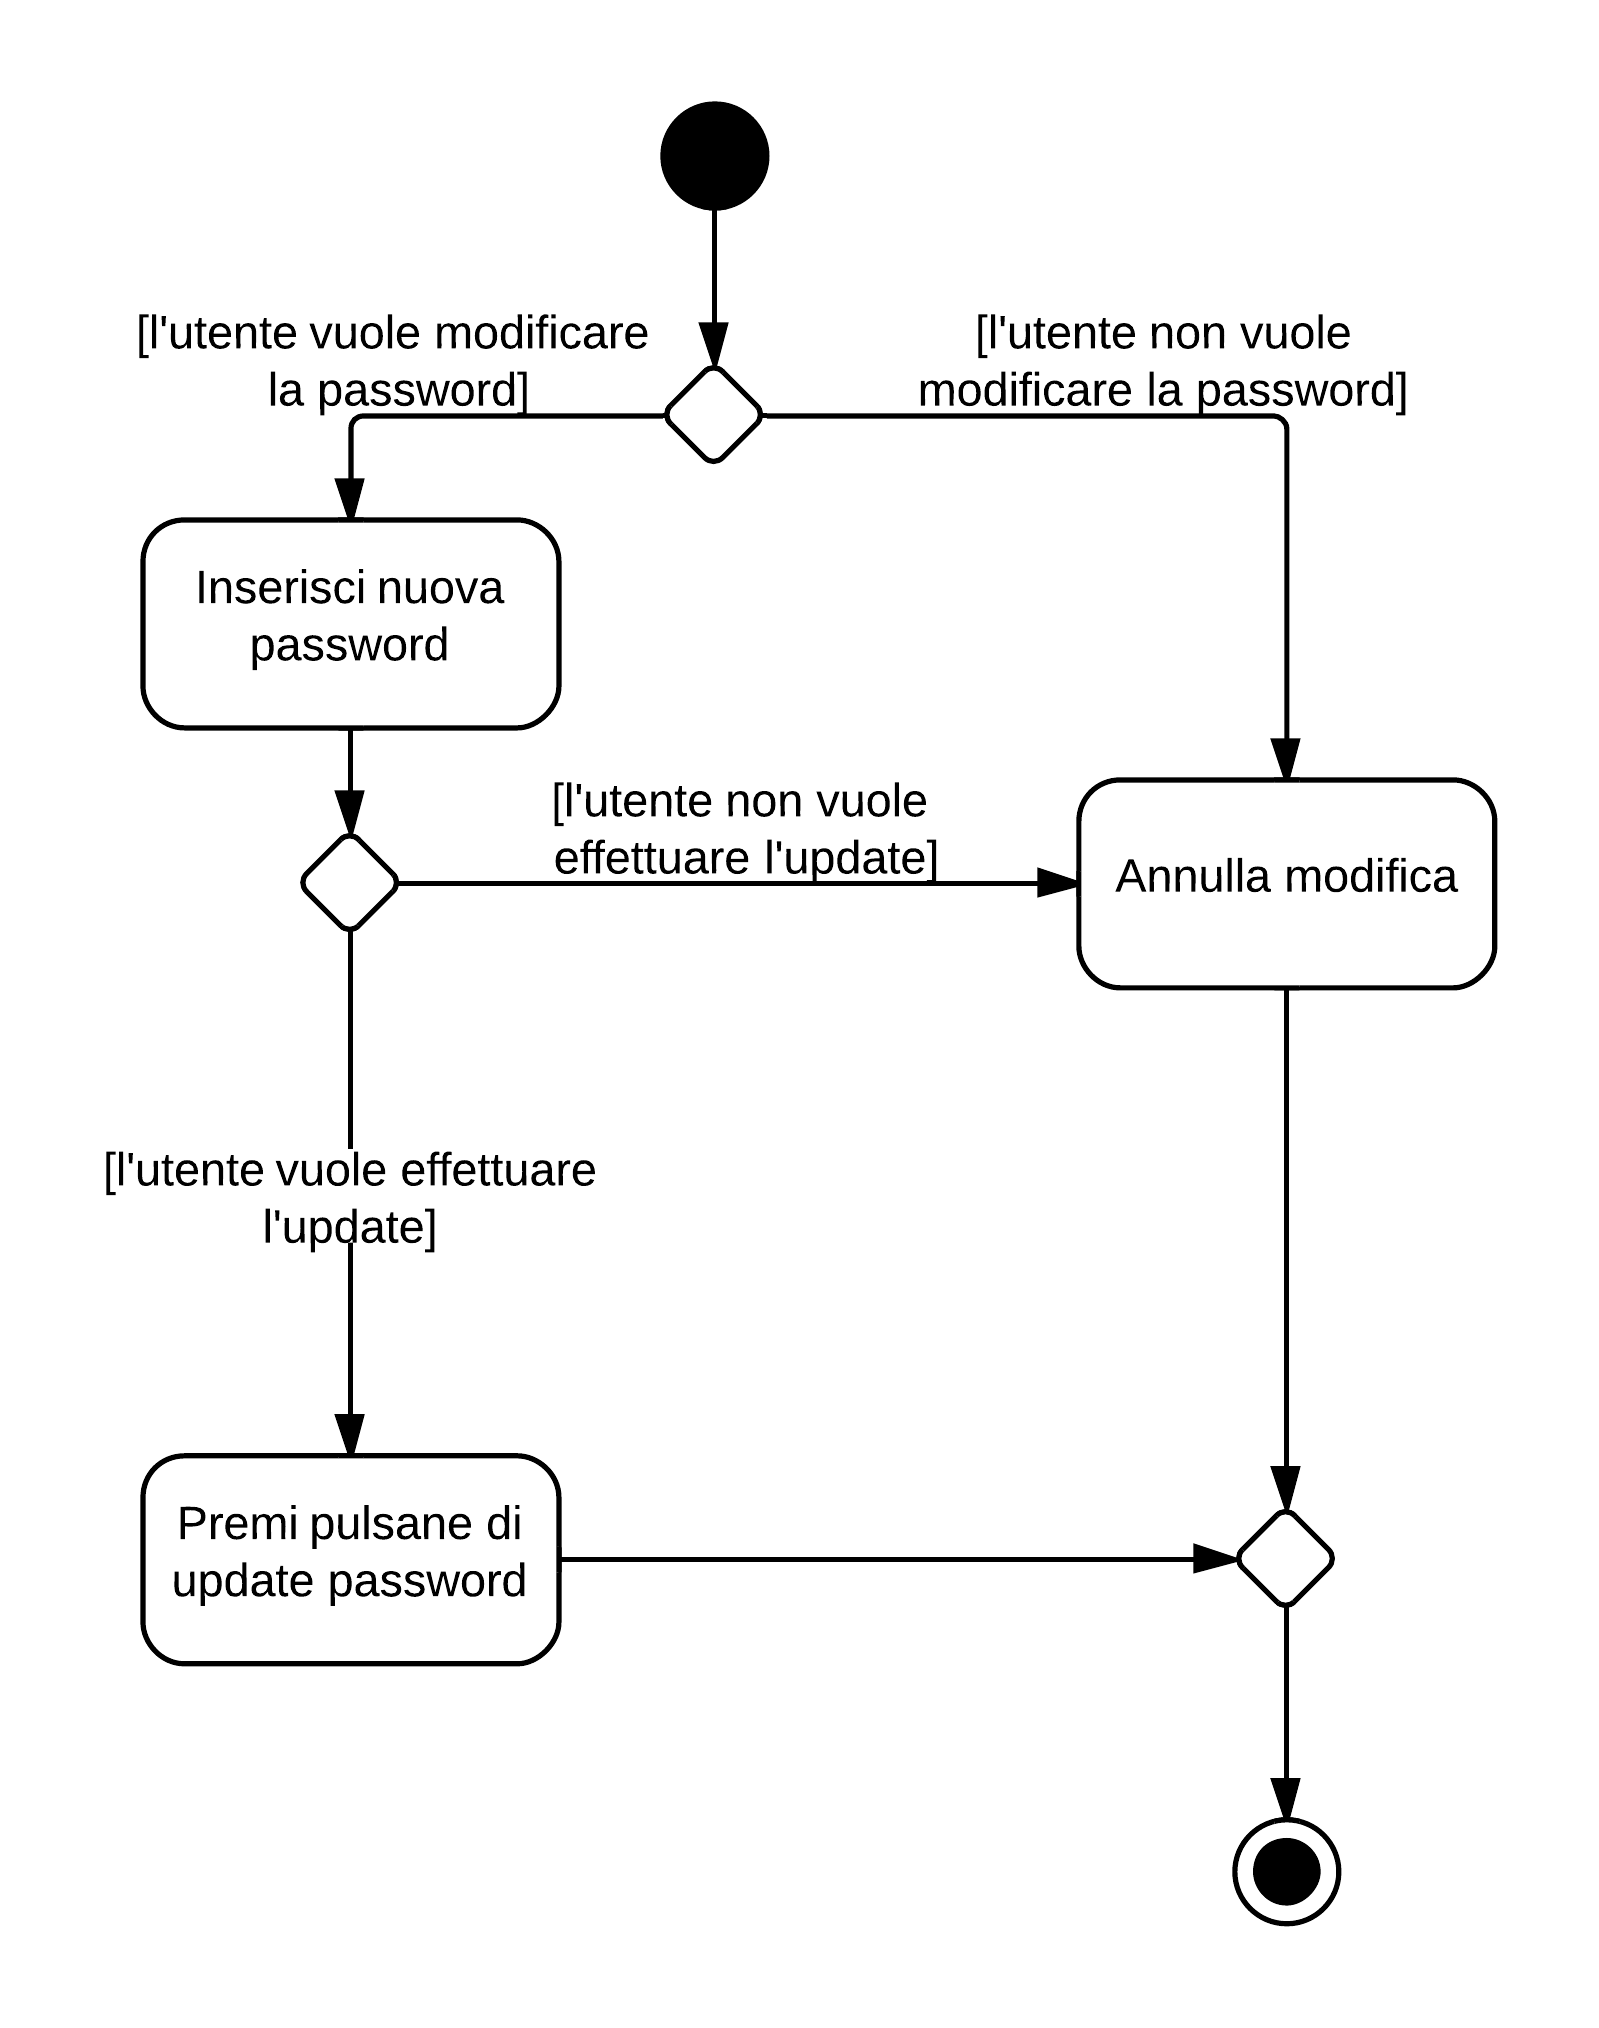
\includegraphics[scale=0.1]{uml/MaaP - Modifica profilo.png}
%\caption{Diagramma di attività - Modifica profilo dell'utente MaaS}
%\end{figure}
%
%In maniera pressoché identica da quanto offerto da un'applicazione \glossario{MaaP} lo sviluppatore entra all'interno della pagina del proprio profilo, dalla quale può modificare la propria password premendo il relativo pulsante. Se decidesse di non voler modificare può in qualsiasi momento annullare le modifiche premendo l'apposito pulsante. Una volta salvate le modifiche il servizio \glossario{MaaS} si occuperà di effettuare correttamente l'upgrade della password nel \glossario{database} delle credenziali.
%
%\subsubsection{Gestisci file di configurazione}
%
%\begin{figure}[H]
%\centering
%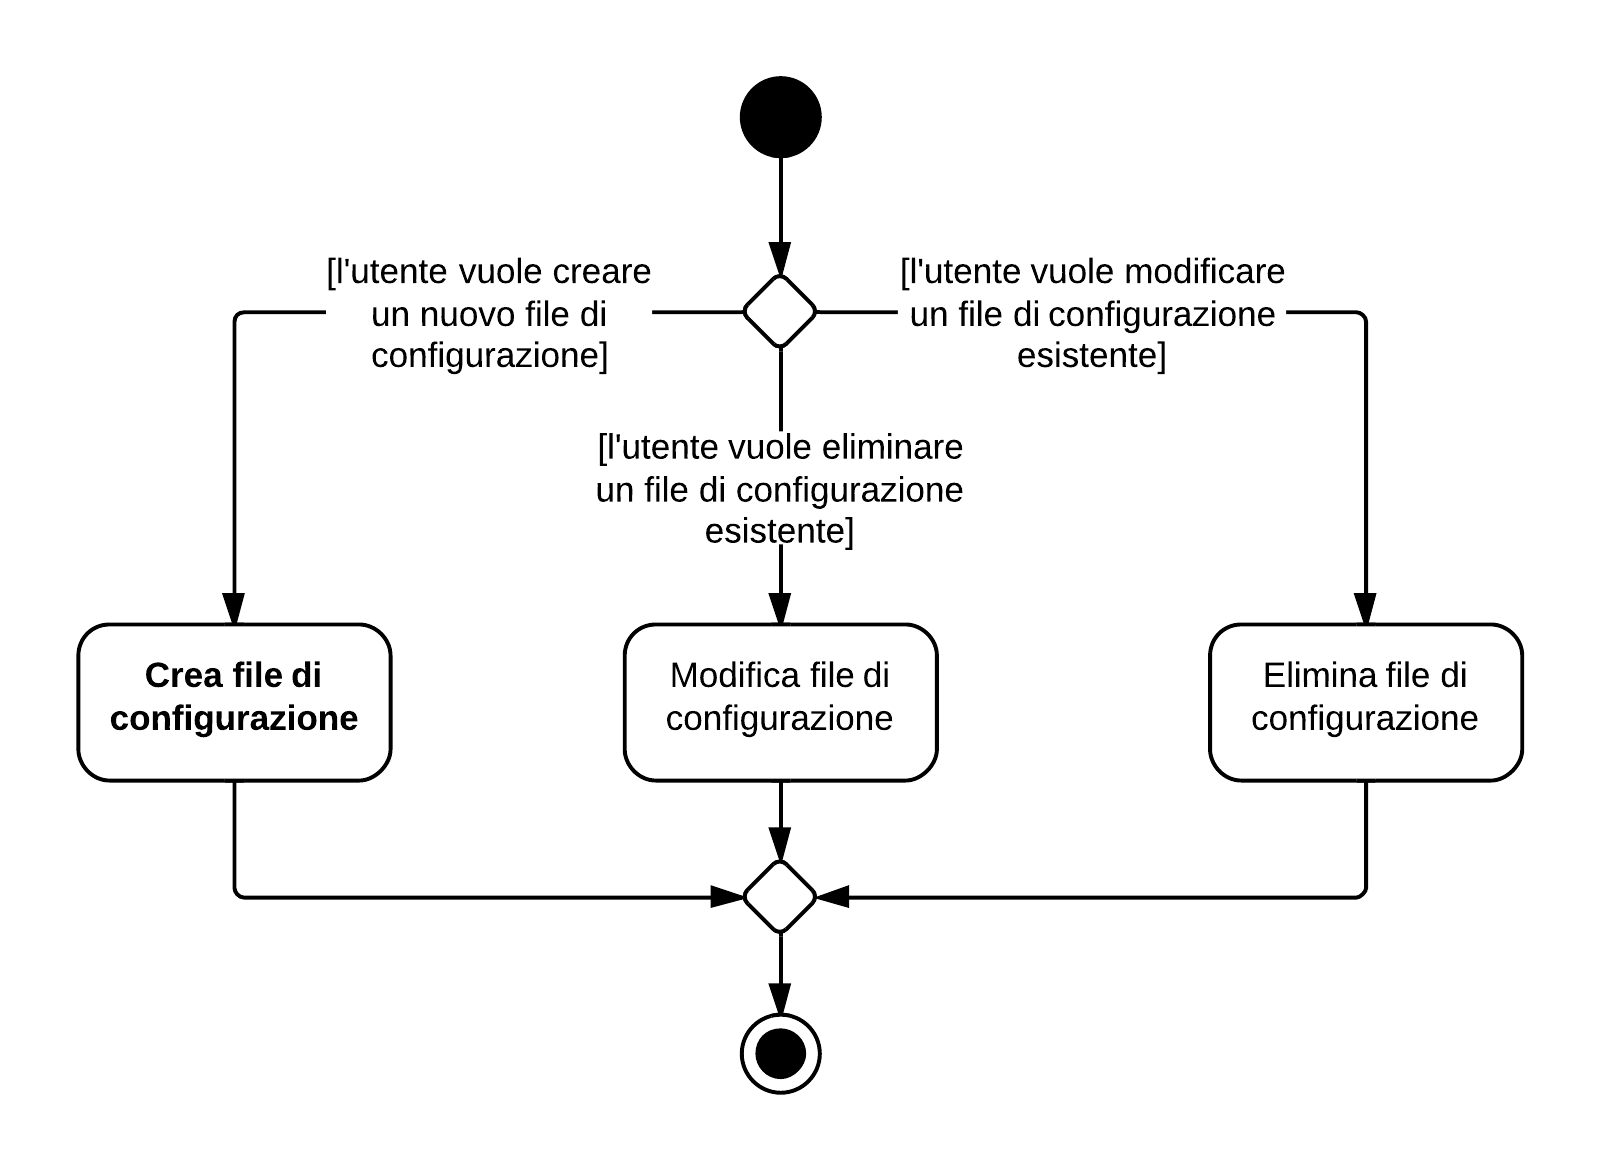
\includegraphics[scale=0.2]{uml/MaaS - Gestisci file di configurazione.png}
%\caption{Diagramma di attività - Gestione dei file di configurazione}
%\end{figure}
%
%L'utente sviluppatore si trova davanti a una pagina in cui visualizza la lista di tutti i propri file di configurazione presenti. Da questa pagina può decidere di:
%
%\begin{itemize}
%
%	\item Creare un nuovo file di configurazione tramite la procedura descritta in seguito;
%	\item Eliminare un file di configurazione esistente;
%	\item Modificare un file di configurazione esistente in maniera analoga alla creazione.
%
%\end{itemize}
%
%\subsubsection{Crea file di configurazione}
%
%\begin{figure}[H]
%\centering
%\includegraphics[scale=0.2]{uml/MaaS - Crea file di configurazione.png}
%\caption{Diagramma di attività - Creazione di un file di configurazione}
%\end{figure}
%
%L'utente sviluppatore si trova davanti a una pagina in cui è presente un editor di testo e un pulsante per effettuare l'upload di un file. Queste sono sostanzialmente le due strade con cui lo sviluppatore può creare un nuovo file di configurazione. Una volta creato o caricato il nuovo file, lo sviluppatore può decidere di procedere al salvataggio oppure annullare la creazione, premendo i relativi pulsanti. Il sistema \glossario{MaaS} nel caso in cui lo sviluppatore decida di procedere alla creazione si occuperà di salvare il file nel sistema.

\subsection{Framework MaaP}

Viene di seguito descritta la procedura con la quale viene creata una nuova applicazione \glossario{MaaP}. Fondamentalmente lo sviluppatore si deve prendere carico di installare tutte le librerie necessarie al corretto funzionamento del \glossario{framework}. Una volta ottenute tutte le \textit{dipendenze} potrà da linea di comando inizializzare un nuovo progetto \glossario{MaaP}. Vengono descritti in seguito i diagrammi di attività per la creazione di una nuova applicazione da parte del sistema.

\subsubsection{Crea nuova applicazione}

\begin{figure}[H]
\centering
\includegraphics[scale=0.2]{uml/Framework - Diagramma di installazione.png}
\caption{Diagramma di attività - Creazione scheletro nuova applicazione}
\end{figure}

Il \glossario{framework} \glossario{MaaP} si occupa di creare tutti i file necessari al corretto funzionamento dell'applicazione nella sua versione di \textit{default}. In particolare si occupa di:

\begin{itemize}

	\item Creare una cartella dove andranno tutti i file relativi al \glossario{front-end};
	\item Creare il file \texttt{package.json} di default, nel quale verrà descritta l'applicazione specificando, ad esempio, il nome, le dipendenze, la versione;
	\item Il file \texttt{server.js} di default, il quale fornisce uno script da eseguire per avviare il server;
	\item Il file \texttt{config.js} di default nel quale viene configurata l'applicazione impostando ad esempio i database;
	\item Una cartella contenente tutti i file \glossario{DSL} che lo sviluppatore andrà a configurare. Di default questa cartella conterrà inizialmente un file \glossario{DSL} di esempio.

\end{itemize}

\subsubsection{Creazione cartella front-end di default}

\begin{figure}[H]
\centering
\includegraphics[scale=0.2]{uml/Framework - Crea cartella front-end di default.png}
\caption{Diagramma di attività - Creazione scheletro nuova applicazione}
\end{figure}

All'interno di questa cartella sono presenti tutti i file di \textit{default} per il corretto funzionamento del front-end. Oltre alla pagina \texttt{index.html} che fungerà da \emph{home} dell'applicazione verrà creato:

\begin{itemize}

	\item La cartella \texttt{js/} all'interno della quale saranno presenti tutti gli script \glossario{javascript} necessari al corretto funzionamento dell'applicazione;
	\item La cartella \texttt{css/} la quale conterrà tutti i fogli di stile per la \textit{presentazione} dell'applicazione;
	\item La cartella \texttt{view/} nella quale saranno presenti i file \textit{html} che fungeranno da \textit{template};
	\item La cartella \texttt{lib/} in cui saranno presenti le librerie \glossario{javascript} già predisposte per il \glossario{front-end}.

\end{itemize}

All'interno di ciascuna cartella saranno presenti inoltre i relativi file di \textit{default}.
\section{Stime di fattibilità e di bisogno di risorse}

Durante l'analisi dell'architettura progettata oltre alle tecnologie e librerie consigliate e richieste nei requisiti, ne sono state ricercate altre per poter avere funzionalità già predisposte e da integrare, garantendo una maggiore fattibilità nel ricoprire le esigenze progettuali. \\
Gli strumenti e le tecnologie integrate a quelle richieste dal capitolato sono : 
\begin{itemize}
\item 
\item 
\end{itemize}

Le tecnologie adottate sono attualmente molto diffuse: si trovano innumerevoli esempi, progetti, librerie, tutorial al riguardo. Da un lato alcune tecnologie non sono del tutto mature, visto che la gran parte dei progetti basati su di esse non raggiungono la versione ``stabile''. Dall'altro lato, però, il supporto della comunità è una grande risorsa: per ogni tipo di problema tecnico è molto facile trovare qualcuno che spieghi come risolverlo. \\
Questo viene in aiuto ai membri del gruppo, la cui maggioranza non aveva sufficienti conoscenze degli strumenti utilizzati per la realizzazione del progetto, conoscenze che sono state approfondite grazie anche alla realizzazione di diversi prototipi interni, relativi all'applicazione front-end, alla realizzazione dell'interfaccia REST e alla realizzazione del parser del linguaggio \glossario{DSL}.
Tali conoscenze continueranno ad essere sviluppate da ognuno dei componenti di \GroupName{}. \\

Gli strumenti definiti durante la progettazione sono ritenuti adeguati per garantire una soddisfacibilità delle necessità progettuali, inoltre sono \glossario{open source} e quindi di facile reperimento rendendo il bisogno di risorse non problematico.



%Le tecnologie e le librerie utilizzate sono attualmente molto diffuse: si trovano innumerevoli esempi, progetti, librerie, tutorial al riguardo. Da un lato la tecnologia non è del tutto matura, visto che la gran parte dei progetti basati su di essa non raggiunge la versione ``stabile''. Dall'altro lato, però, il supporto della comunità è una grande risorsa: per ogni tipo di problema tecnico è molto facile trovare qualcuno che spieghi come risolverlo.
%nel corso della progettazione sono state realizzati diversi prototipi interni, relativi all'applicazione front-end, alla realizzazione dell'interfaccia REST, alla realizzazione del parser del linguaggio DSL. 

\section{Design pattern}

Un \glossario{Design Pattern} descrive problemi che si ripetono molteplici volte nel nostro ambiente. Oltre al problema descrive anche soluzioni eleganti ad esso e i risultati che si ottengono nell'applicarlo. È fondamentale per qualsiasi progettista conoscere a fondo i \glossario{Design Pattern}, in quanto facilita l'attività di progettazione, favorisce la riusabilità e dà benefici enormi in termini di manutenibilità. Fondamentalmente possiamo suddividere i \glossario{Design Pattern} in quattro categorie:

\begin{itemize}

	\item \textbf{\glossario{Design Pattern} architetturali}, che esprimono schemi di base per impostare l'organizzazione strutturale di un sistema software;
	\item \textbf{\glossario{Design Pattern} creazionali}, che forniscono un'astrazione del processo di istanziazione degli oggetti;
	\item \textbf{\glossario{Design Pattern} strutturali}, che si occupano delle modalità di composizione di classi e oggetti per formare strutture complesse; 
	\item \textbf{\glossario{Design Pattern} comportamentali}, che si occupano di algoritmi e dell'assegnamento di responsabilità tra oggetti collaboranti.

\end{itemize}

Per un approfondimento e un richiamo teorico dei \glossario{Design Pattern} utilizzati nel progetto \glossario{MaaP} si rimanda all'Appendice \ref{appendice-pattern}. In seguito verranno descritti i \glossario{Design Pattern} implementati.

\subsection{Design Pattern Architetturali}

\subsubsection{MVC}

\begin{itemize}

	\item \textbf{Scopo}: Questo pattern è utilizzato per separare le responsabilità dell'applicazione a diversi componenti e permettere di fare una chiara divisione presentazione, struttura dei dati e operazioni su di essi.
	\item \textbf{Utilizzo}: Viene utilizzato dall'applicazione principalmente per delegare il ruolo di presentazione dei dati al \glossario{front-end}, lasciando al \glossario{back-end} la gestione della logica dell'applicazione (autenticazione, corrispondenza tra \glossario{API} e operazioni sui dati) e la logica di business.
	
\end{itemize}

\subsubsection{MVW}

\begin{itemize}

	\item \textbf{Scopo}: È un \glossario{Design Pattern} simile a \glossario{MVC} che permette di avere una corrispondenza più diretta e automatica tra la \textit{view} e il \textit{model}. L'acronimo \glossario{MVW} sta per \textit{Model-View-Whatever}, dove \textit{Whatever}, secondo i progettisti di \glossario{Angular.js}, indica "\textit{whatever works for you}".
	\item \textbf{Utilizzo}: È il \glossario{Design Pattern} utilizzato dal \glossario{framework} \glossario{Angular.js}, con il quale viene sviluppata la parte \glossario{front-end} dell'applicazione \glossario{MaaP}.

\end{itemize}

\subsubsection{Middleware} 

\begin{itemize}

	\item \textbf{Scopo}: Si è scelto di utilizzare questo \glossario{Design Pattern} per fornire un \textit{intermediario} tra i vari componenti software dell'applicazione in modo da semplificare notevolmente la loro connessione e collaborazione. Questo pattern in generale è molto utile nello sviluppo e nella gestione di di sistemi distribuiti complessi, e in questo contesto il progetto \glossario{MaaP} si colloca perfettamente.
	\item \textbf{Utilizzo}: Viene utilizzato dal \glossario{framework} \glossario{Express} attraverso il modulo \textit{connect} per fornire una libreria di funzioni comuni. Definisce una serie di \textit{livelli} (o funzioni) per gestire le varie richieste dell'applicazione e richiamare i rispettivi \textit{handler}. Tutti i componenti del middleware sono collegati l'uno con l'altro e ricevono a turno una richiesta in ingresso, finché uno di questi non decide di partire con l'elaborazione per poi chiamare la funzione \texttt{next}. Come si può notare è molto legato a \glossario{Chain of Responsibility}, che verrà descritto in seguito. Tutti i componenti di \glossario{Express} vengono utilizzati con il metodo \texttt{use} di \glossario{Express}. Nella progettazione architetturale è utilizzato nel package \texttt{Back-End::Lib::Middleware}.

\end{itemize}

\begin{figure}[H]
\centering \includegraphics[width=1\textwidth]{patterns/contestualizzazione/middleware.png}
\caption{Contestualizzazione di Middleware}
\label{fig:mvc}
\end{figure}

\subsection{Design Pattern Creazionali}

\subsubsection{Registry}

\begin{itemize}

	\item \textbf{Scopo}: Viene utilizzato per ottenere oggetti a partire da altri oggetti che hanno un'associazione con esso. Questa ricerca viene effettuata tramite una \textit{classe registro}, che conterrà una funzione di ricerca in base a una chiave.
	\item \textbf{Utilizzo}: Le diverse \glossario{Collection} presenti nell'applicazione si differenziano per il loro nome. Utilizzando questo pattern, quando arriva una richiesta la classe che lo implementa sarà in grado di fornire il file \glossario{DSL} corretto in quanto possiederà al suo interno un registro sul quale sarà possibile effettuare una ricerca. È implementato nella classe \texttt{Back-End::Lib::DSLModel}. Alla sua creazione verrà caricato il registro. Questa classe inoltre conterrà un metodo di ricerca e un metodo di caricamento del file DSL.

\end{itemize}

\begin{figure}[H]
\centering \includegraphics[width=0.8\textwidth]{patterns/contestualizzazione/registry.png}
\caption{Contestualizzazione di Registry}
\label{fig:mvc}
\end{figure}

\subsubsection{Factory method}

\begin{itemize}

	\item \textbf{Scopo}: Nel contesto di \glossario{Node.js} questo pattern viene usato creare una classe e restituire una sua istanza attraverso una \textit{funzione factory} che verrà esportata dal modulo. In questo modo si potrà costruire e ottenere qualsiasi classe definita in un modulo.
	\item \textbf{Utilizzo}: Alle basi del \textit{routing}, che utilizza la rappresentazione \glossario{REST}, vi sarà un controller associato per l'esecuzione delle diverse funzioni a seconda dell'URL indicato. In base a quest'ultimo dev'essere istanziata l'apposita classe che si occuperà di effettuare le sue funzioni. Per creare un oggetto di quella classe ci si avvale di una classe \textit{factory}, la quale si occuperà di invocare la costruzione dell'oggetto. Nell'architettura del progetto il pattern è implementato nella classe \texttt{Back-End::Lib::Controller::ControllerFactory}.

\end{itemize}

\begin{figure}[H]
\centering \includegraphics[width=0.8\textwidth]{patterns/contestualizzazione/factory-method.png}
\caption{Contestualizzazione di Factory Method}
\label{fig:mvc}
\end{figure}

\subsubsection{Singleton}

\begin{itemize}

	\item \textbf{Scopo}: Viene utilizzato per le classi che devono avere un'unica istanza durante l'esecuzione dell'applicazione;
	\item \textbf{Utilizzo}: Ogni modulo di \glossario{Node.js} è nativamente un singleton, perché viene caricato al primo \code{require} e poi tutti i successivi riferiscono allo stesso.

\end{itemize}

\subsection{Design Pattern Strutturali}

\subsubsection{Facade}

\begin{itemize}

	\item \textbf{Scopo}: Viene utilizzato per rendere visibili solamente alcune cose agli altri oggetti ed avere un unico punto di accesso semplificato a un sottosistema fornendo un'interfaccia di alto livello e minimizzando dunque le comunicazioni e le dipendenze.
	\item \textbf{Utilizzo}: Viene utilizzato all'interno della classe \\ \texttt{Back-End::Lib::Middleware::MiddlewareLoader}, la quale utilizza \textit{facade} per nascondere l'esistenza di tutti i \glossario{middleware} alla \texttt{ServerApp}. In questo modo le richieste vengono delegate agli oggetti appropriati senza che la classe cliente conosca le classi del sottosistema. Sarà il \textit{Facade} che si occuperà di trasferire la comunicazione all'oggetto appropriato.
\end{itemize}

\begin{figure}[H]
\centering \includegraphics[width=1\textwidth]{patterns/contestualizzazione/facade1.png}
\caption{Contestualizzazione di Facade in \texttt{Back-End::Lib::Middleware::MiddlewareLoader}}
\label{fig:mvc}
\end{figure}

\subsection{Design Pattern Comportamentali}

\subsubsection{Chain of Responsibility}
\label{chain-of-responsibility}

\begin{itemize}

	\item \textbf{Scopo}: Viene utilizzato per far sì che un oggetto a cui viene effettuata una richiesta possa esaudire le richieste di più oggetti. In questo modo si evita l'accoppiamento fra il mittente di una richiesta e il destinatario. Tutti gli oggetti destinatari della richiesta sono \textit{concatenati} tra di loro. Ogni nodo della catena se può esaudire la richiesta la effettua, altrimenti delega l'onere al nodo successivo. La catena viene attraversata finché un nodo non può eseguire l'ordine del mittente. 
	\item \textbf{Utilizzo}: \glossario{Express} usa \textit{chain of Responsibility} per la gestione dei \glossario{middleware} e del \glossario{routing}. Come già accennato è particolarmente legato al pattern \textit{Middleware}. Viene utilizzato nella nostra architettura all'interno del package \texttt{Back-End::Lib::Middleware}. La classe \texttt{Back-End::Lib::Middleware::MiddlewareHandler} gestisce la richiesta scorrendo tutta la lista delle sottoclassi e richiamando il metodo \texttt{next} finché una di queste non può soddisfarla.

\end{itemize}

\begin{figure}[H]
\centering \includegraphics[width=0.4\textwidth]{patterns/contestualizzazione/chain-of-responsability.png}
\caption{Contestualizzazione di Chain of Responsibility}
\label{fig:mvc}
\end{figure}

\subsubsection{Strategy}

\begin{itemize}

	\item \textbf{Scopo}: Questo pattern serve per definire una famiglia di algoritmi e renderli intercambiabili, in modo che essi possano variare indipendentemente dal client che ne fa utilizzo. In un progetto software che guarda al futuro e che verrà manutenuto è fondamentale poter effettuare modifiche alle procedure in modo non intrusivo.
	\item \textbf{Utilizzo}: Viene utilizzato all'interno della classe \\ \texttt{Back-End::Lib::DSLModel::DSLInterpreterStrategy} in modo da permettere in futuro cambiamenti all'algoritmo di interpretazione del \glossario{DSL} senza dover intervenire sulla classe che ne fa uso, ovvero \texttt{Back-End::Lib::DSLModel::DSLDomain}.

\end{itemize}

\begin{figure}[H]
\centering \includegraphics[width=0.8\textwidth]{patterns/contestualizzazione/strategy.png}
\caption{Contestualizzazione di Strategy}
\label{fig:mvc}
\end{figure}

\subsubsection{Command}

\begin{itemize}

	\item \textbf{Scopo}: Viene usato per parametrizzare gli oggetti rispetto a un'azione da compiere.
	\item \textbf{Utilizzo}: Viene utilizzato nel \glossario{package} \texttt{Back-End::DSLModel} per definire le azioni personalizzate da intraprendere sulle \glossario{Collection} o sui \glossario{Document}. In particolare \\ \texttt{Back-End::DSLModel::DocumentAction} e \texttt{Back-End::DSLModel::CollectionAction} rappresentano ciascuno il componente \textit{Command} del pattern (applicato in due contesti diversi). La componente \textit{ConcreteCommand} del pattern consiste in una delle due precedenti classi estese dinamicamente, ridefinendo un metodo.

\end{itemize}
\section{Tracciamento}
\subsection{Tracciamento requisiti-classi}

\begin{center}
      \bgroup
      \def\arraystretch{1.8}
      \begin{longtable}{ | p{3cm} | p{11cm} | }
    \hline
    
      \cellcolor[gray]{0.9} \textbf{Requisito} & \cellcolor[gray]{0.9} \textbf{Classe} \\ \hline
      
	RA1O 1 & Front-end::Controllers::LoginController \newline Front-end::Controllers::LoginView \newline 
			Back-end::Lib::Controller::Service::ProfileService \newline
			Back-end::Lib::Controller::Middleware::Authentication\\ \hline 
			
	RA1O 1.1 & Front-end::Controllers::LoginController \newline Front-end::Controllers::LoginView \\ \hline 
	RA1O 1.2 & Front-end::Controllers::LoginController \newline Front-end::Controllers::LoginView \\ \hline      

	RA1O 1.3 & Back-end::Lib::Controller::Middleware::Authentication  \newline 
			Back-end::Lib::Controller::Service::UserService \newline 
			Back-end::Lib::Model::UserModel  \newline \\ \hline  
    
    RA1O 1.3.1 & Front-end::Model::ErrorModel \newline Back-end::Lib::Utils::MaapError  \newline \\ \hline 
           
    RA1O 1.3.2 & Back-end::Lib::Controller::Middleware::Authentication \newline
        			Back-end::Lib::Controller::Service::ProfileService \newline
        			Back-end::Lib::Controller::Middleware::Router \newline
        			Front-end::Controllers::DashboardController \newline
        			Front-end::Controllers::DashboardView  \newline  \\ \hline 
        				
        				     
    RA1O 2 & Back-end::Lib::Controller::Service::ForgotService \newline
    			Back-end::Lib::Model::UserModel \newline
    			Front-end::Services::ForgotResetController \newline
    			Front-end::Model::RequestResetModel  \newline  \\ \hline   
    			   
    RA1O 2.1 & Front-end::Controllers::ForgotRequestController \newline  \\ \hline   
       
    RA1O 2.2 & Back-end::Lib::Controller::Service::ForgotService \newline
    			  			Back-end::Lib::Utils::Mailer \newline
    			  			Back-end::Lib::View::ForgotMailView \newline  \\ \hline     
    			   
     
    RA1D 3 & Front-end::Controllers::DashboardController \newline Front-end::Controllers::DashboardView \\ \hline  
        
    RA1O 4 & Front-end::Controllers::CollectionController \newline 
    			Back-end::Lib::Controller::Service::CollectionService  \newline \\ \hline   
       
    RA1O 4.1 & Back-end::Lib::Controller::Service::IndexService \newline
    			Back-end::Lib::Model::DSLModel::IndexModel \newline 
    			Back-end::Lib::Model::DSLModel::Row \newline
    			Back-end::Lib::Model::DSLModel::Column \newline
    			Front-end::Controllers::CollectionController \newline 
    			Front-end::Model::CollectionView \newline  \\ \hline   
       
    RA1O 4.1.1 & Front-end::Controllers::CollectionController \newline 
    Front-end::Model::CollectionView \newline  \\ \hline 
	
	RA1O 4.1.2 & Front-end::Controllers::CollectionController \newline 
    Front-end::Model::CollectionView \newline  \\ \hline 
    
    RA1O 4.1.3 & Front-end::Controllers::CollectionController \newline 
    Front-end::Model::CollectionView \newline  \\ \hline 	
	         
    RA1O 5 & Front-end::Controllers::ShowController \newline
    			 Front-end::Model::ShowModel \newline
    			 Back-end::Lib::Model::DSLModel::DocumentSchema \newline
    			 Back-end::Lib::Model::DSLModel::ShowModel \newline
    			 Back-end::Lib::Controller::Service::ShowService \newline  \\ \hline   
    			  
    RA1O 5.1 & Back-end::Lib::Controller::Service::ShowService \newline
    			Back-end::Lib::Model::DSLModel::DocumentSchema \newline 
    			Back-end::Lib::Model::DSLModel::ShowModel \\ \hline
    			   
    RA1O 5.3 &
    			Front-end::Controllers::ShowController \newline
    			Back-end::Lib::Controller::Service::ShowService \newline
    			Back-end::Lib::Model::DSLModel::ShowModel \newline \\ \hline      
    
    RA1O 6 & Back-end::Lib::Controller::Service::UserService \newline  
    			Back-end::Lib::Model::UserModel \newline Front-end::Controllers::UsersListController  \\ \hline  
        
    RA1O 6.1 & Front-end::Controllers::UserController \newline Back-end::Lib::Controller::Service::UserService \newline Back-end::Lib::Model::UserModel \\ \hline   
       
    RA1O 6.1.1 & Front-end::Controllers::UserController \newline  \\ \hline     
     
    RA1O 6.1.1.1 & Front-end::Controllers::UserController \newline  \\ \hline
        
    RA1O 6.1.1.2 & Front-end::Controllers::UserController \newline  \\ \hline
        
    RA1O 6.1.1.3 & Front-end::Controllers::UserController \newline  \\ \hline
       
    RA1O 6.1.2 & Back-end::Lib::Controller::Service::UserService \newline Back-end::Lib::Model::UserModel \newline Front-end::Controllers::UserController \newline Front-end::Model::UserModel \newline  \\ \hline     
    
    
    RA1O 6.2 & Front-end::Controllers::UsersListController \newline Back-end::Lib::Controller::Service::UserService \\ \hline     
     
    RA1O 6.2.1 & Back-end::Lib::Controller::Service::UserService \newline Front-end::Controllers::UserController \newline  \\ \hline      
    RA1O 6.2.2 & Front-end::Controllers::UserController \newline  \\ \hline      
      
    RF1O 7 & Back-end::Lib::Model::DSLModel::DSLDomain \newline Back-end::Lib::Model::DSLModel::DSLInterpreterStrategy \newline Back-end::Lib::Model::DSLModel::CollectionModel \newline Back-end::Lib::Controller::Middleware::DSLLoaderHandler \\ \hline      
    
    RF1O 8 & Back-end::Lib::ServerApp \newline  \\ \hline   
       
    RF1O 8.1  & Back-end::DeveloperProject::ProjectApp \newline  \\ \hline  
        
    RF1O 8.1.1 & Back-end::DeveloperProject::ProjectApp \newline  \\ \hline      
    RF1O 8.1.2 & Back-end::DeveloperProject::ProjectApp \newline Back-end::DeveloperProject::Config::ProjectConfig \newline  \\ \hline        
           
    RF1O 9 & Back-end::Lib::Model::DSLModel::DSLCollectionModel\newline  \\ \hline      
    
    RF1O 9.1 & Back-end::Lib::Model::DSLModel::IndexModel \newline  \\ \hline   
       
    RF1O 9.1.1 & Back-end::Lib::Model::DSLModel::IndexModel \newline Back-end::Lib::Model::DSLModel:ObjectUtils \newline
    				Back-end::Lib::Utils::AttributeReader \\ \hline      
    
    RF1O 9.1.2 & Back-end::Lib::Model::DSLModel::IndexModel \newline Back-end::Lib::Utils::AttributeReader  \\ \hline      
    
    RF1O 9.1.3 &  Back-end::Lib::Model::DSLModel::IndexModel \newline Back-end::Lib::Utils::AttributeReader \\ \hline   
       
    RF1O 9.1.4 & Back-end::Lib::Model::DSLModel::IndexModel \newline Back-end::Lib::Utils::AttributeReader  \\ \hline 
         
    RF1O 9.1.5 & Back-end::Lib::Utils::AttributeReader \newline Back-end::Lib::Model::DSLModel:ObjectUtils \\ \hline      
    
    RF1O 9.1.6 & Back-end::Lib::Utils::AttributeReader \newline Back-end::Lib::Model::DSLModel:ObjectUtils \\ \hline      
    
    RF1O 9.1.7 & Back-end::Lib::Model::DSLModel::IndexModel \newline Back-end::Lib::Utils::AttributeReader \newline  \\ \hline
          
    RF1O 9.2 & Back-end::Lib::Model::DSLModel::ShowModel \newline  \\ \hline   
       
    RF1O 9.2.1 & Back-end::Lib::Model::DSLModel::ShowModel \newline Back-end::Lib::Utils::AttributeReader  \\ \hline       
    
    RF1O 9.2.2  & Back-end::Lib::Model::DSLModel::ShowModel \newline Back-end::Lib::Utils::AttributeReader  \\ \hline     
     
    RF1O 9.2.3 & Back-end::Lib::Model::DSLModel::ShowModel \newline Back-end::Lib::Utils::AttributeReader \\ \hline      
    
    RF1O 9.2.4 & Back-end::Lib::Utils::AttributeReader \newline Back-end::Lib::Model::DSLModel::ShowModel \\ \hline      
            
    RA1D 11 & Back-end::Lib::Controller::Service::UserService \newline Back-end::Lib::Model::UserModel  \\ \hline
    RA1D 12 & Back-end::Lib::Controller::Service::ProfileService  \\ \hline
    RA1D 13 & Back-end::Lib::Controller::Service::ProfileService  \newline Back-end::Lib::Model::UserModel \\ \hline
    
    RF1O 14 & Back-end::DeveloperProject::Config::ProjectConfig \newline  \\ \hline      
    RF1O 14.1 & Back-end::DeveloperProject::Config::ProjectConfig \newline  \\ \hline      
         
    RA1O 18 & Back-end::Lib::Model::DSLModel::DSLInterpreterStrategy \newline
    			 Back-end::Lib::Model::DSLModel::DSLInterpreterStrategy::ConcreteDSLInterpreter \newline 
    			Back-end::Lib::Utils::MaapError  \\ \hline      
      \caption{Requisiti-Classi}
      \end{longtable}
      \egroup
      \end{center}  
\clearpage

\subsection{Tracciamento classi-requisiti}

\begin{center}
      \bgroup
      \def\arraystretch{1.8}
      \begin{longtable}{ | p{11cm} | p{3cm} | }
    \hline
    
      \cellcolor[gray]{0.9} \textbf{Classe} & \cellcolor[gray]{0.9} \textbf{Requisito} \\ \hline
    Back-end::Lib::Controller::Service::ServiceFactory & \\ \hline
	Back-end::Lib::Controller::Service::UserService & RA1O 1.3 \newline RA1O 6.1.2 \newline RA1O 6.2 \newline RA1O 6.2.1  \newline 
	RA1D 11  \\ \hline
	
	Back-end::Lib::Controller::Service::IndexService & RA1O 4.1 \\ \hline
	
	Back-end::Lib::Controller::Service::ProfileService & RA1O 1 \newline RA1O 1.3.2  \newline RA1D 12 \newline RA1D 13 \\ \hline

	Back-end::Lib::Controller::Service::ShowService & RA1O 5 \newline RA1O 5.1 \newline RA1O 5.3 \\ \hline
	
	Back-end::Lib::Controller::Service::ForgotService & RA1O 2 \newline RA1O 2.2 \\ \hline
	
	Back-end::Lib::Controller::Service::CollectionService & RA1O 4 \\ \hline
	
	Back-end::Lib::Controller::Middleware::MiddlewareLoader & \\ \hline

	Back-end::Lib::Controller::Middleware::Authentication & RA1O 1 \newline RA1O 1.3 \newline RA1O 1.3.2 \\ \hline
	
	Back-end::Lib::Controller::Middleware::DSLLoaderHandler & RF1O 7 \\ \hline
	
	Back-end::Lib::Controller::Middleware::NotFoundHandler & \\ \hline
	
	Back-end::Lib::Controller::Middleware::ErrorHandler & \\ \hline
	
	Back-end::Lib::Controller::Middleware::Router & \\ \hline
	
	Back-end::Lib::Model::UserModel & RA1O 1.3 \newline RA1O 2 \newline RA1O 6 \newline RA1O 6.1 \newline 
										RA1O 6.1.2 \newline RA1D 11 \newline RA1D 13 \\ \hline
	
	Back-end::Lib::Model::DSLModel::DocumentSchema & RA1O 5 \newline RA1O 5.1 \\ \hline
	
	Back-end::Lib::Model::DSLModel:ObjectUtils & RF1O 9.1.5 \newline RF1O 9.1.6 \\ \hline
	
	Back-end::Lib::Model::DSLModel::ShowModel & RF1O 9.2 \newline RF1O 9.2.1 \newline RF1O 9.2.2 \newline
												 RF1O 9.2.3 \newline RF1O 9.2.4 \\ \hline

	Back-end::Lib::Model::DSLModel::Row & RA1O 4.1 \\ \hline
	
	Back-end::Lib::Model::DSLModel::Column & RA1O 4.1 \\ \hline
	
	Back-end::Lib::Model::DSLModel::IndexModel & RA1O 4.1 \newline RF1O 9.1 \newline RF1O 9.1.2 \newline
												 RF1O 9.1.3 \newline RF1O 9.1.4  \newline RF1O 9.1.7  \\ \hline
	
	Back-end::Lib::Model::DSLModel::DSLDomain & RF1O 7 \\ \hline
	
	Back-end::Lib::Model::DSLModel::DSLConcreteStrategy & RA1O 18 \\ \hline
	
	Back-end::Lib::Model::DSLModel::DSLCollectionModel & RF1O 9 \\ \hline
	
	Back-end::Lib::View::ForgotMailView & RA1O 2.2 \\ \hline
	
	Back-end::Lib::Utils::Mailer & RA1O 2.2 \\ \hline
	
	Back-end::Lib::Utils::MaapError & RA1O 1.3.1 \\ \hline
	
	Back-end::Lib::Utils::AttributeReader & RF1O 9.1.1 \newline RF1O 9.1.2 \newline RF1O 9.1.3 \newline RF1O 9.1.4 \newline 
										RF1O 9.1.5 \newline RF1O 9.1.6 \newline RF1O 9.1.7 \\ \hline

	Back-end::Lib::Config & \\ \hline
	
	Back-end::DeveloperProject::Config::ProjectConfig & RF1O 14 \newline RF1O 14.1 \\ \hline
	
	Back-end::DeveloperProject::ProjectApp & \\ \hline
	

	\caption{Classi-requisito}
      \end{longtable}
      \egroup
      \end{center}  
\clearpage

\subsection{Tracciamento metodi-test}
   \begin{center}
\begin{longtable}{ | p{12cm} | p{2cm} | }
\hline
 \textbf{Classe e Metodo} & \textbf{Test} \\ \hline
Back-end::Lib::Controller::Middleware::Router::handler() &  \\ \hline
Back-end::Lib::Controller::Middleware::Router::init() &  \\ \hline
Back-end::Lib::Controller::Middleware::Authentication::handler() &  \\ \hline
Back-end::Lib::Controller::Middleware::Authentication::authenticate() &  \\ \hline
Back-end::Lib::Controller::Middleware::Authentication::init() &  \\ \hline
Back-end::Lib::Controller::Middleware::Authentication::requireAdmin() &  \\ \hline
Back-end::Lib::Controller::Middleware::ErrorHandler::handler() &  \\ \hline
Back-end::Lib::Controller::Middleware::MiddlewareLoader::init() &  \\ \hline
Back-end::Lib::Controller::Middleware::DSLLoaderHandler::init() &  \\ \hline
Back-end::Lib::View::ForgotMailView::buildForgotMail() &  \\ \hline
Back-end::Lib::Controller::Controller::ProfileController::login() &  \\ \hline
Back-end::Lib::Controller::Middleware::DSLLoaderHandler::browseFileSystem() &  \\ \hline
Back-end::Lib::Controller::Controller::UserController::registerUser() & TU - 49 \\ \hline
Back-end::Lib::Controller::Controller::UserController::insertUser() & TU - 50 \\ \hline
Back-end::Lib::Controller::Controller::UserController::userIdShowPage() & TU - 51 \\ \hline
Back-end::Lib::Controller::Controller::ForgotController::passwordResetRequest() &  \\ \hline
Back-end::Lib::Controller::Controller::ControllerFactory::getCollectionController() &  \\ \hline
Back-end::Lib::Controller::Controller::ControllerFactory::getProfileController() &  \\ \hline
Back-end::Lib::Controller::Controller::ControllerFactory::getAuthController() &  \\ \hline
Back-end::Lib::Controller::Controller::ControllerFactory::getForgotController() &  \\ \hline
Back-end::Lib::Controller::Controller::ControllerFactory::getUserController() &  \\ \hline
Back-end::Lib::Controller::Controller::ControllerFactory::getShowController() &  \\ \hline
Back-end::Lib::Controller::Controller::ControllerFactory::getIndexController() &  \\ \hline
Back-end::Lib::Controller::Controller::UserController::updateLevel() & TU - 53 \\ \hline
Back-end::Lib::Utils::Mailer::Mailer() & TU - 54 \\ \hline
Back-end::Lib::Controller::Controller::ProfileController::logout() &  \\ \hline
Back-end::Lib::Utils::Mailer::sendEmail() &  \\ \hline
Back-end::Lib::Controller::Middleware::Authentication::requireLogged() &  \\ \hline
Back-end::Lib::Controller::Middleware::Authentication::requireNotLogged() &  \\ \hline
Back-end::Lib::Controller::Middleware::Authentication::requireSuperAdmin() &  \\ \hline
Back-end::Lib::Controller::Middleware::NotFoundHandler::handler() &  \\ \hline
Back-end::Lib::Model::DSLModel::DSLCollectionModel::DSLCollectionModel() & TU - 28 \\ \hline
Back-end::Lib::Model::DSLModel::DSLCollectionModel::getCollectionName() & TU - 29 \\ \hline
Back-end::Lib::Model::DSLModel::DSLCollectionModel::getIndexModel() & TU - 30 \\ \hline
Back-end::Lib::Model::DSLModel::DSLCollectionModel::getShowModel() & TU - 31 \\ \hline
Back-end::Lib::Controller::Controller::ProfileController::getProfile() &  \\ \hline
Back-end::Lib::Controller::Controller::ProfileController::updatePassword() &  \\ \hline
Back-end::Lib::Model::DSLModel::DSLDomain::getErrors() & TU - 16 \\ \hline
Back-end::Lib::Utils::MaapError::toString() & TU - 7 \\ \hline
Back-end::Lib::Model::UserModel::\underline{getUserById}() & TU - 24 \\ \hline
Back-end::Lib::Config::getServerPort() &  \\ \hline
Back-end::Lib::Config::getServerStaticPath() &  \\ \hline
Back-end::Lib::Config::getUserDbUri() &  \\ \hline
Back-end::Lib::ServerApp::start() &  \\ \hline
Back-end::Lib::Model::UserModel::\underline{getUserList}() & TU - 18 \\ \hline
Back-end::Lib::Utils::MaapError::toJson() & TU - 6 \\ \hline
Back-end::DeveloperProject::ProjectApp::\underline{start}() &  \\ \hline
Back-end::Lib::Config::getEnvironment() &  \\ \hline
Back-end::Lib::Config::getDataDbUri() &  \\ \hline
Back-end::Lib::Config::getSmtpService() &  \\ \hline
Back-end::Lib::Config::getSmtpAuth() &  \\ \hline
Back-end::Lib::Controller::Controller::ShowController::getShowPage() &  \\ \hline
Back-end::Lib::Controller::Controller::ShowController::deleteDocument() &  \\ \hline
Back-end::Lib::Model::DSLModel::DSLDomain::registerCollection() & TU - 14 \\ \hline
Back-end::Lib::Model::DSLModel::DSLDomain::getCollectionModel() & TU - 15 \\ \hline
Back-end::Lib::Model::UserModel::\underline{registerUser}() & TU - 19 \\ \hline
Back-end::Lib::Model::UserModel::\underline{deleteUser}() & TU - 22 \\ \hline
Back-end::Lib::Model::UserModel::\underline{updateLevel}() & TU - 20 \\ \hline
Back-end::Lib::Model::UserModel::\underline{createUser}() & TU - 21 \\ \hline
Back-end::Lib::Model::UserModel::\underline{updatePassword}() & TU - 23 \\ \hline
Back-end::Lib::Model::DSLModel::DSLInterpreterStrategy::ConcreteDSLInterpreter::init() & TU - 26 \\ \hline
Back-end::Lib::Model::DSLModel::DSLInterpreterStrategy::ConcreteDSLInterpreter::loadDSLFile() & TU - 27 \\ \hline
Back-end::Lib::Utils::MaapError::toError() & TU - 8 \\ \hline
Back-end::Lib::Controller::Controller::UserController::usersList() & TU - 52 \\ \hline
Back-end::Lib::Model::DSLModel::Attribute::getLabel() & TU - 43 \\ \hline
Back-end::Lib::Model::DSLModel::Attribute::getName() & TU - 44 \\ \hline
Back-end::Lib::Model::DSLModel::ShowModel::ShowModel() & TU - 38 \\ \hline
Back-end::Lib::Model::DSLModel::Attribute::getTransformation() & TU - 45 \\ \hline
Back-end::Lib::Model::DSLModel::Attribute::isSelectable() & TU - 46 \\ \hline
Back-end::Lib::ServerApp::ServerApp() & TU - 4 \\ \hline
Back-end::Lib::Utils::MaapError::MaapError() & TU - 5 \\ \hline
Front-end::Controllers::UsersListController::deleteUser() &  \\ \hline
Front-end::Controllers::UsersListController::createUser() & TU - 10 \\ \hline
Front-end::Controllers::LoginController::login() & TU - 11 \\ \hline
Back-end::Lib::Model::DSLModel::DSLDomain::DSLDomain() & TU - 12 \\ \hline
Back-end::Lib::Model::DSLModel::DSLDomain::loadDSLFile() & TU - 13 \\ \hline
Back-end::Lib::Model::UserModel::init() & TU - 17 \\ \hline
Back-end::Lib::Model::DSLModel::DSLInterpreterStrategy::ConcreteDSLInterpreter::DSLConcreteStrategy() & TU - 25 \\ \hline
Back-end::Lib::Model::DSLModel::DSLCollectionModel::setIndexModel() & TU - 32 \\ \hline
Back-end::Lib::Model::DSLModel::DSLCollectionModel::setShowModel() & TU - 33 \\ \hline
Back-end::Lib::Model::DSLModel::IndexModel::IndexModel() & TU - 34 \\ \hline
Back-end::Lib::Model::DSLModel::IndexModel::addAttribute() & TU - 35 \\ \hline
Back-end::Lib::Model::DSLModel::IndexModel::getAttributes() & TU - 36 \\ \hline
Back-end::Lib::Model::DSLModel::IndexModel::getData() & TU - 37 \\ \hline
Back-end::Lib::Model::DSLModel::ShowModel::addAttribute() & TU - 39 \\ \hline
Back-end::Lib::Model::DSLModel::ShowModel::getAttributes() & TU - 40 \\ \hline
Back-end::Lib::Model::DSLModel::ShowModel::getData() & TU - 41 \\ \hline
Back-end::Lib::Config::getDSLPath() &  \\ \hline
Back-end::Lib::Model::DSLModel::Attribute::Attribute() & TU - 42 \\ \hline
Back-end::Lib::Model::DSLModel::Attribute::isSortable() & TU - 47 \\ \hline
Back-end::Lib::Controller::Controller::UserController::deleteUser() & TU - 48 \\ \hline
Back-end::Lib::Controller::Controller::IndexController::getIndexPage() & TU - 54 \\ \hline
\caption{Metodi-Test}
\end{longtable}
\end{center}


%\appendix
%\input{appendice}

\end{document}
